%\chapter{Analytical Size Distribution, Form Factors, and Structure factors}
%\label{SDFFSQ}

\chapter{Form Factors}
\label{formfactor}

 The different types of form factors are
selected in the different submenus. Below one finds how they are
ordered. The definitions of the individual form factors are
defined below. Under the submenu \texttt{other functions} all form
factors under development and those functions, which are not at
all form factors but which have been implemented for some other
purposes are listed.
\begin{itemize}
\item Background
\item auxiliary and transition functions
\begin{itemize}
%  \item \texttt{Background}
%  \item \texttt{Sigmoid}
%  \item \texttt{Gaussian Cumulative}
%  \item \texttt{Lorentzian Cumulative}
%  \item \texttt{Logistic Dose Response}
%  \item \texttt{Log-Normal Cumulative}
%  \item \texttt{Extreme Value Cumulative}
%  \item \texttt{Pulse Cumulative}
  \item \texttt{p(r) -> 4 pi r\^{}2 sin(qr)/(qr)}
  \item \texttt{gamma(r) -> 4 pi sin(qr)/(qr)}
\end{itemize}
\item Spheres \& Shells (\ref{sect:Spheres_Shells})
\begin{itemize}
\item \texttt{Sphere} (\ref{sect:sphere})
\item \texttt{Spherical Shell i} (\ref{sect:spherical_shell_i})
\item \texttt{Spherical Shell ii} (\ref{sect:spherical_shell_ii})
\item \texttt{Spherical Shell iii} (\ref{sect:spherical_shell_iii})
\item \texttt{MultiLamellarVesicle} (\ref{sect:MultiLamellarVesicle})
\item \texttt{RNDMultiLamellarVesicle}
\item \texttt{RNDMultiLamellarVesicle2}
\item \texttt{BiLayeredVesicle} (\ref{sect:BilayeredVesicle})
\item \texttt{LinShell} (\ref{sect:LinShell})
\item \texttt{LinShell2} (\ref{sect:LinShell2})
\item \texttt{ExpShell} (\ref{sect:ExpShell})
\end{itemize}
\item ellipsoidal obj. (\ref{sect:EllipsoidalObjects})
\begin{itemize}
\item \texttt{Ellipsoid i} \ref{sect:Ellipsoid_i}
\item \texttt{Ellipsoid ii} \ref{sect:Ellipsoid_ii}
\item \texttt{EllipsoidalCoreShell} \ref{sect:EllipsoidalCoreShell}
\item \texttt{triaxEllShell1} \ref{sect:triaxEllShell1}
\end{itemize}
\item polymers \& micelles (\ref{sect:Polymers_Micelles})
\begin{itemize}
\item polymer chains
\begin{itemize}
\item \texttt{Gauss} (\ref{sect:GaussCoil})
\item \texttt{Gauss2} (\ref{sect:GaussCoil})
\item \texttt{Gauss3} (\ref{sect:GaussCoil})
\item \texttt{GaussPoly} (\ref{sect:GaussCoil})
\item \texttt{generalized Gaussian coil} (\ref{sect:generalized_gaussian_coil})
\item \texttt{generalized Gaussian coil 2} (\ref{sect:generalized_gaussian_coil2})
\item \texttt{generalized Gaussian coil 3} (\ref{sect:generalized_gaussian_coil3})
\end{itemize}
\item polymer stars
\begin{itemize}
\item \texttt{BenoitStar} (\ref{sect:Benoit})
\item \texttt{PolydisperseStar} (\ref{sect:PolydisperseStar})
\item \texttt{Dozier} (\ref{sect:DozierStar1})
\item \texttt{Dozier2} (\ref{sect:DozierStar2})
\end{itemize}
\item polymer rings
\begin{itemize}
\item \texttt{FlexibleRingPolymer} (\ref{sect:FlexibleRingPolymer})
\item \texttt{$m$MemberedTwistedRing} (\ref{sect:mMemberedTwistedRing})
\item \texttt{DaisyLikeRing} (\ref{sect:DaisyLikeRing})
\end{itemize}
\item spherical \& ellipsoidal micelles
\begin{itemize}
\item \texttt{SPHERE+Chains(RW)\_Nagg} (\ref{sect:SphericalMicelles})
\item \texttt{SPHERE+Chains(RW)\_Rc} (\ref{sect:SphericalMicelles})
\item \texttt{SPHERE+Chains(RW)} (\ref{sect:SphericalMicelles})
\item \texttt{SPHERE+Chains(SAW)\_Nagg}
\item \texttt{SPHERE+Chains(SAW)\_Rc}
\item \texttt{SPHERE+Chains(SAW)}
\item \texttt{SPHERE+R\^{}-a\_Nagg} (\ref{sect:SPHERE+R_ma})
\item \texttt{SPHERE+R\^{}-a\_Rc} (\ref{sect:SPHERE+R_ma})
\item \texttt{SPHERE+R\^{}-a} (\ref{sect:SPHERE+R_ma})
\item \texttt{SPHERE\_smooth\_interface+R\^{}-a\_Nagg}
\item \texttt{SPHERE\_smooth\_interface+R\^{}-a\_Rc}
\item \texttt{ELL+Chains(RW)\_Nagg} (\ref{sect:ELLMicelles})
\item \texttt{ELL+Chains(RW)\_Rc} (\ref{sect:ELLMicelles})
\item \texttt{ELL+Chains(RW)} (\ref{sect:ELLMicelles})
\item \texttt{SphereWithGaussChains}
\item \texttt{BlockCopolymerMicelle}
\end{itemize}
\item cylindrical \& rod-like micelles
\begin{itemize}
\item \texttt{CYL+Chains(RW)\_Nagg} (\ref{sect:CylMicelles})
\item \texttt{CYL+Chains(RW)\_Rc} (\ref{sect:CylMicelles})
\item \texttt{CYL+Chains(RW)} (\ref{sect:CylMicelles})
\item \texttt{WORM+Chains(RW)\_nagg} (\ref{sect:WormLikeMicelles})
\item \texttt{WORM+Chains(RW)\_Rc} (\ref{sect:WormLikeMicelles})
\item \texttt{WORM+Chains(RW)}(\ref{sect:WormLikeMicelles})
\item \texttt{ROD+Chains(RW)\_nagg} (\ref{sect:RodLikeMicelles})
\item \texttt{ROD+Chains(RW)\_Rc} (\ref{sect:RodLikeMicelles})
\item \texttt{ROD+Chains(RW)} (\ref{sect:RodLikeMicelles})
\item \texttt{ROD+R\^{}-a\_nagg} (\ref{sect:ROD+R_ma})
\item \texttt{ROD+R\^{}-a\_Rc} (\ref{sect:ROD+R_ma})
\item \texttt{ROD+R\^{}-a} (\ref{sect:ROD+R_ma})
\item \texttt{ROD+Exp\_nagg}
\item \texttt{ROD+Exp\_Rc}
\item \texttt{ROD+Exp}
\end{itemize}
\item local planar micelles (sheets, ULV)
\begin{itemize}
\item \texttt{DISC+Chains(RW)\_nagg}
\item \texttt{DISC+Chains(RW)\_Lc}
\item \texttt{DISC+Chains(RW)}
\item \texttt{SphULV+Chains(RW)\_nagg}
\item \texttt{SphULV+Chains(RW)\_tc}
\item \texttt{SphULV+Chains(RW)}
\item \texttt{EllULV+Chains(RW)\_nagg}
\item \texttt{EllULV+Chains(RW)\_tc}
\item \texttt{EllULV+Chains(RW)}
\item \texttt{CylULV+Chains(RW)\_nagg}
\item \texttt{CylULV+Chains(RW)\_tc}
\item \texttt{CylULV+Chains(RW)}
\end{itemize}
\item wormlike structures
\begin{itemize}
\item \texttt{WormLikeChainEXV} (\ref{sect:WormLikeChain})
\item \texttt{KholodenkoWorm} (\ref{sect:KholodenkoWorm})
\end{itemize}
\end{itemize}
\item cluster obj. (\ref{sect:ClusteredObjects})
\begin{itemize}
\item \texttt{Fisher-Burford} (\ref{sect:MassFractal})
\item \texttt{MassFractExp}(\ref{sect:MassFractal})
\item \texttt{MassFractGauss} (\ref{sect:MassFractal})
\item \texttt{Aggregate (Exp(-x\^{}a) Cut-Off)} (\ref{sect:MassFractal})
\item \texttt{Aggregate (OverlapSph Cut-Off)} (\ref{sect:MassFractal})
\item \texttt{DLCAggregation} (\ref{sect:MassFractal})
\item \texttt{RLCAggregation} (\ref{sect:MassFractal})
\item \texttt{MassFractOverlappingSph} (\ref{sect:MassFractal})
\item \texttt{StackDiscs} (\ref{sect:StackedDiscs})
\item \texttt{DumbbellShell} (\ref{sect:DumbbellShell})
\item \texttt{two\_attached\_spheres}
\item \texttt{DoubleShellChain} (\ref{sect:DoubleShellChain})
\item \texttt{TetrahedronDoubleShell} (\ref{sect:TetrahedronDoubleShell})
\end{itemize}
\item non-particular structures
\begin{itemize}
\item \texttt{OrnsteinZernike} (\ref{sect:Zernike})
\item \texttt{BroadPeak} (\ref{sect:BroadPeak})
\item \texttt{TeubnerStrey} (\ref{sect:TeubnerStrey})
\item \texttt{DAB} (\ref{sect:DAB})
\item \texttt{Spinodal} (\ref{sect:Spinodal})
\item \texttt{BeaucageExpPowLaw} (\ref{sect:Beaucage})
\item \texttt{BeaucageExpPowLaw2} (\ref{sect:Beaucage})
\item \texttt{Guinier} \ref{sec:generalizedGuinier}
\end{itemize}
\item cylindrical obj. (\ref{sect:CylindricalObjects})
\begin{itemize}
\item \texttt{Disc} (\ref{sect:Disc})
\item Rod (\ref{sect:Rod})
\item \texttt{EllCylShell}
\item \texttt{PorodCylinder} (\ref{sect:PorodCylinder})
\item \texttt{LongCylinder} (\ref{sect:LongCylinder})
\item \texttt{FlatCylinder} (\ref{sect:flatCylinder})
\item \texttt{Cylinder} (\ref{sect:Cylinder})
\item \texttt{LongCylShell} (\ref{sect:randomCylindricalShell})
\item \texttt{CylShell1} (\ref{sect:randomCylindricalShell})
\item \texttt{CylShell2} (\ref{sect:randomCylindricalShell})
\item \texttt{ellCylShell1} (\ref{sect:random_ellCylinderShell})
\item \texttt{ellCylShell2} (\ref{sect:random_ellCylinderShell})
\item \texttt{alignedCylShell}
\item \texttt{partly aligned CylShell}
\item \texttt{Torus} (\ref{sect:Torus})
\end{itemize}
\begin{itemize}
  \item anisotropic obj.
  \begin{itemize}
    \item Pcs(Q) for planar obj.
    \begin{itemize}
      \item \texttt{Pcs:homogenousXS} (\ref{sect:homogeneousXS})
      \item \texttt{Pcs:TwoInfinitelyThinPlates} (\ref{sect:TwoInfinitelyThinPlates})
      \item \texttt{Pcs:LayeredCentroSymmetricXS}(\ref{sect:LayeredCentroSymmetricXS})
      \item \texttt{Pcs:BiLayerGauss} (\ref{sect:BiLayerGauss})
      \item \texttt{Pcs:Plate+Chains(RW)}
    \end{itemize}
    \item Pcs(Q) for cylindrical obj.
    \begin{itemize}
      \item \texttt{Pcs:homogeneousXS}
      \item \texttt{Pcs:CylindricalShell}
      \item \texttt{Pcs:Rod+Chains(RW)}
      \item \texttt{Pcs:ellCylSh}
    \end{itemize}
  \end{itemize}
\end{itemize}
\item plane obj.
\begin{itemize}
  \item \texttt{homogenousXS} (\ref{sect:homogeneousXS})
  \item \texttt{SphSh+SD+homoXS}
  \item \texttt{EllSh+SD+homoXS}
  \item \texttt{EllSh+SD+homoXS(S)}
  \item \texttt{CylSh+SD+homoXS}
  \item \texttt{Disc+homoXS}
  \item \texttt{TwoInfinitelyThinPlates} (\ref{sect:TwoInfinitelyThinPlates})
  \item \texttt{LayeredCentroSymmetricXS} (\ref{sect:LayeredCentroSymmetricXS})
  \item \texttt{BiLayerGauss} (\ref{sect:BiLayerGauss})
\end{itemize}
\item sheared objects
\begin{itemize}
  \item \texttt{ShearedCylinder} (\ref{sect:ShearedCylinderHayterPenfold})
  \item \texttt{ShearedCylGauss} (\ref{sect:ShearedCylinderGaussian})
\end{itemize}
\item magnetic objects (\ref{sect:MagScatt})
\begin{itemize}
  \item \texttt{MagneticShellPsi} (\ref{sect:MagShellPsi})
  \item \texttt{MagneticShellAniso} (\ref{sect:MagShellAniso})
  \item \texttt{MagneticShellCrossTerm} (\ref{sect:MagShellCrossTerm})
  \item \texttt{SuperparamagneticFFpsi} (\ref{sect:superparFFpsi})
  \item \texttt{SuperparamagneticFFAniso} (\ref{sect:superparFFAniso})
  \item \texttt{SuperparamagneticFFIso} (\ref{sect:superparFFIso})
  \item \texttt{SuperparamagneticFFCrossTerm} (\ref{sect:superparFFCrossTerm})
\end{itemize}
\item Mie FF for SLS (\ref{sect:LorenzMieSLS})
\begin{itemize}
  \item \texttt{MieSphere} (\ref{sect:MieSphere})
  \item \texttt{MieShell} (\ref{sect:MieShell})
\end{itemize}
\item Peaks (\ref{ch:peaks})
\begin{itemize}
  \item Amplitude Functions
  \begin{itemize}
    \item \texttt{Beta (Amplitude)} (\ref{sec:BetaAmplitude})
    \item \texttt{Chi-squared (Amplitude)} (\ref{sec:ChiSquaredAmplitude})
    \item \texttt{Erfc (Amplitude)} (\ref{sec:ErfcPeakAmplitude}
    \item \texttt{Error (Amplitude)} (\ref{sec:ErrorPeakAmplitude})
    \item \texttt{exponentially modified Gaussian (Amplitude)} (\ref{sec:ExponentiallyModifiedGaussianAmplitude})
    \item \texttt{Extreme Value (Amplitude)} (\ref{sec:ExtremeValueAmplitude})
    \item \texttt{F-variance (Amplitude)} (\ref{sec:FVarianceAmplitude})
    \item \texttt{Gamma (Amplitude)} (\ref{sec:GammaDistrAmplitude})
    \item \texttt{Gaussian (Amplitude)} (\ref{sec:GaussianNormalAmplitude})
    \item \texttt{Gaussian-Lorentzian cross product (Amplitude)} (\ref{sec:GaussianLorentzianCrossProductAmplitude})
    \item \texttt{Gaussian-Lorentzian sum (Amplitude)} (\ref{sec:GaussianLorentzianSumAmplitude})
    \item \texttt{generalized Gaussian 1 (Amplitude)} (\ref{sec:generalizedGaussian1Amplitude})
    \item \texttt{generalized Gaussian 2 (Amplitude)} (\ref{sec:generalizedGaussian2Amplitude})
    \item \texttt{Giddings (Amplitude)} (\ref{sec:GiddingsAmplitude})
    \item \texttt{Inverted Gamma (Amplitude)} (\ref{sec:InvertedGammaAmplitude})
    \item \texttt{Kumaraswamy (Amplitude)} (\ref{sec:KumaraswamyAmplitude})
    \item \texttt{Laplace (Amplitude)} (\ref{sec:LaplaceAmplitude})
    \item \texttt{Logistic (Amplitude)} (\ref{sec:LogisticAmplitude})
    \item \texttt{LogLogistic (Amplitude)} (\ref{sec:LogLogisticAmplitude})
    \item \texttt{LogNormal, 4 parameters (Amplitude)} (\ref{sec:LogNormal4ParameterArea})
    \item \texttt{LogNormal (Amplitude)} (\ref{sec:LogNormalAmplitude})
    \item \texttt{Lorentzian (Amplitude)} (\ref{sec:LorentzianAmplitude})
    \item \texttt{Pearson IV (Amplitude)} (\ref{sec:PearsonIVAmplitude})
    \item \texttt{Pearson VII (Amplitude)} (\ref{sec:PearsonVIIAmplitude})
    \item \texttt{pulse (Amplitude)}  (\ref{sec:PulseAmplitude})
    \item \texttt{pulse with 2nd width (Amplitude)}  (\ref{sec:pulsewith2ndwidthAmplitude})
    \item \texttt{pulse with power term (Amplitude)}  (\ref{sec:pulsewithpowertermAmplitude})
    \item \texttt{Student-t (Amplitude)} (\ref{sec:Student-tAmplitude})
    \item \texttt{Voigt (Amplitude)} (\ref{sec:VoigtAmplitude})
    \item \texttt{Weibull (Amplitude)} (\ref{sec:WeibullAmplitude})
  \end{itemize}
  \item Area Functions
  \begin{itemize}
    \item \texttt{Beta (Area)} (\ref{sec:BetaArea})
    \item \texttt{Chi-squared (Area)} (\ref{sec:ChiSquaredArea})
    \item \texttt{Erfc (Area)} (\ref{sec:ErfcPeakArea}
    \item \texttt{Error (Area)} (\ref{sec:ErrorPeakArea})
    \item \texttt{exponentially modified Gaussian (Area)} (\ref{sec:ExponentiallyModifiedGaussianArea})
    \item \texttt{Extreme Value (Area)} (\ref{sec:ExtremeValueArea})
    \item \texttt{F-variance (Area)} (\ref{sec:FVarianceArea})
    \item \texttt{Gamma (Area)} (\ref{sec:GammaDistrArea})
    \item \texttt{Gaussian (Area)} (\ref{sec:GaussianNormalArea})
    \item \texttt{Gaussian-Lorentzian cross product (Area)} (\ref{sec:GaussianLorentzianCrossProductArea})
    \item \texttt{Gaussian-Lorentzian sum (Area)} (\ref{sec:GaussianLorentzianSumArea})
    \item \texttt{generalized Gaussian 1 (Area)} (\ref{sec:generalizedGaussian1Area})
    \item \texttt{generalized Gaussian 2 (Area)} (\ref{sec:generalizedGaussian2Area})
    \item \texttt{Giddings (Area)} (\ref{sec:GiddingsArea})
    \item \texttt{Haarhoff - Van der Linde (Area)} (\ref{sec:HaarhoffVanderLindeArea})
    \item \texttt{Half Gaussian Modified Gaussian (Area)} (\ref{sec:HalfGaussianModifiedGaussianArea})
    \item \texttt{Inverted Gamma (Area)} (\ref{sec:InvertedGammaArea})
    \item \texttt{Kumaraswamy (Area)} (\ref{sec:KumaraswamyArea})
    \item \texttt{Laplace (Area)} (\ref{sec:LaplaceArea})
    \item \texttt{Logistic (Area)} (\ref{sec:LogisticArea})
    \item \texttt{LogNormal, 4 parameters (Area)} (\ref{sec:LogNormal4ParameterArea})
    \item \texttt{LogNormal (Area)} (\ref{sec:LogNormalArea})
    \item \texttt{Lorentzian (Area)} (\ref{sec:LorentzianArea})
    \item \texttt{Pearson IV (Area)} (\ref{sec:PearsonIVArea})
    \item \texttt{Pearson VII (Area)} (\ref{sec:PearsonVIIArea})
    \item \texttt{pulse (Area)}  (\ref{sec:PulseArea})
    \item \texttt{pulse with 2nd width (Area)}  (\ref{sec:pulsewith2ndwidthArea})
    \item \texttt{pulse with power term (Area)}  (\ref{sec:pulsewithpowertermArea})
    \item \texttt{Student-t (Area)} (\ref{sec:Student-tArea})
    \item \texttt{Voigt (Area)} (\ref{sec:VoigtArea})
    \item \texttt{Weibull (Area)} (\ref{sec:WeibullArea})
  \end{itemize}
\end{itemize}
\item other functions
\begin{itemize}
\item Langevin
\item DoubleShell\_withSD
\item SuperparStroboPsi
\item SuperparStroboPsi2
\item SuperparStroboPsiSQ
\item SuperparStroboPsiBt1
\item SuperparStroboPsiLx
\item SuperparStroboPsiL2x
\item DLS\_Sphere\_RDG
\item Robertus1
\item J\"{u}lichMicelle
\end{itemize}
\end{itemize}


\clearpage
\section{Spheres \& Shells}
\label{sect:Spheres_Shells}

\subsection{Sphere}
\label{sect:sphere} ~\\

\begin{figure}[htb]
\begin{center}
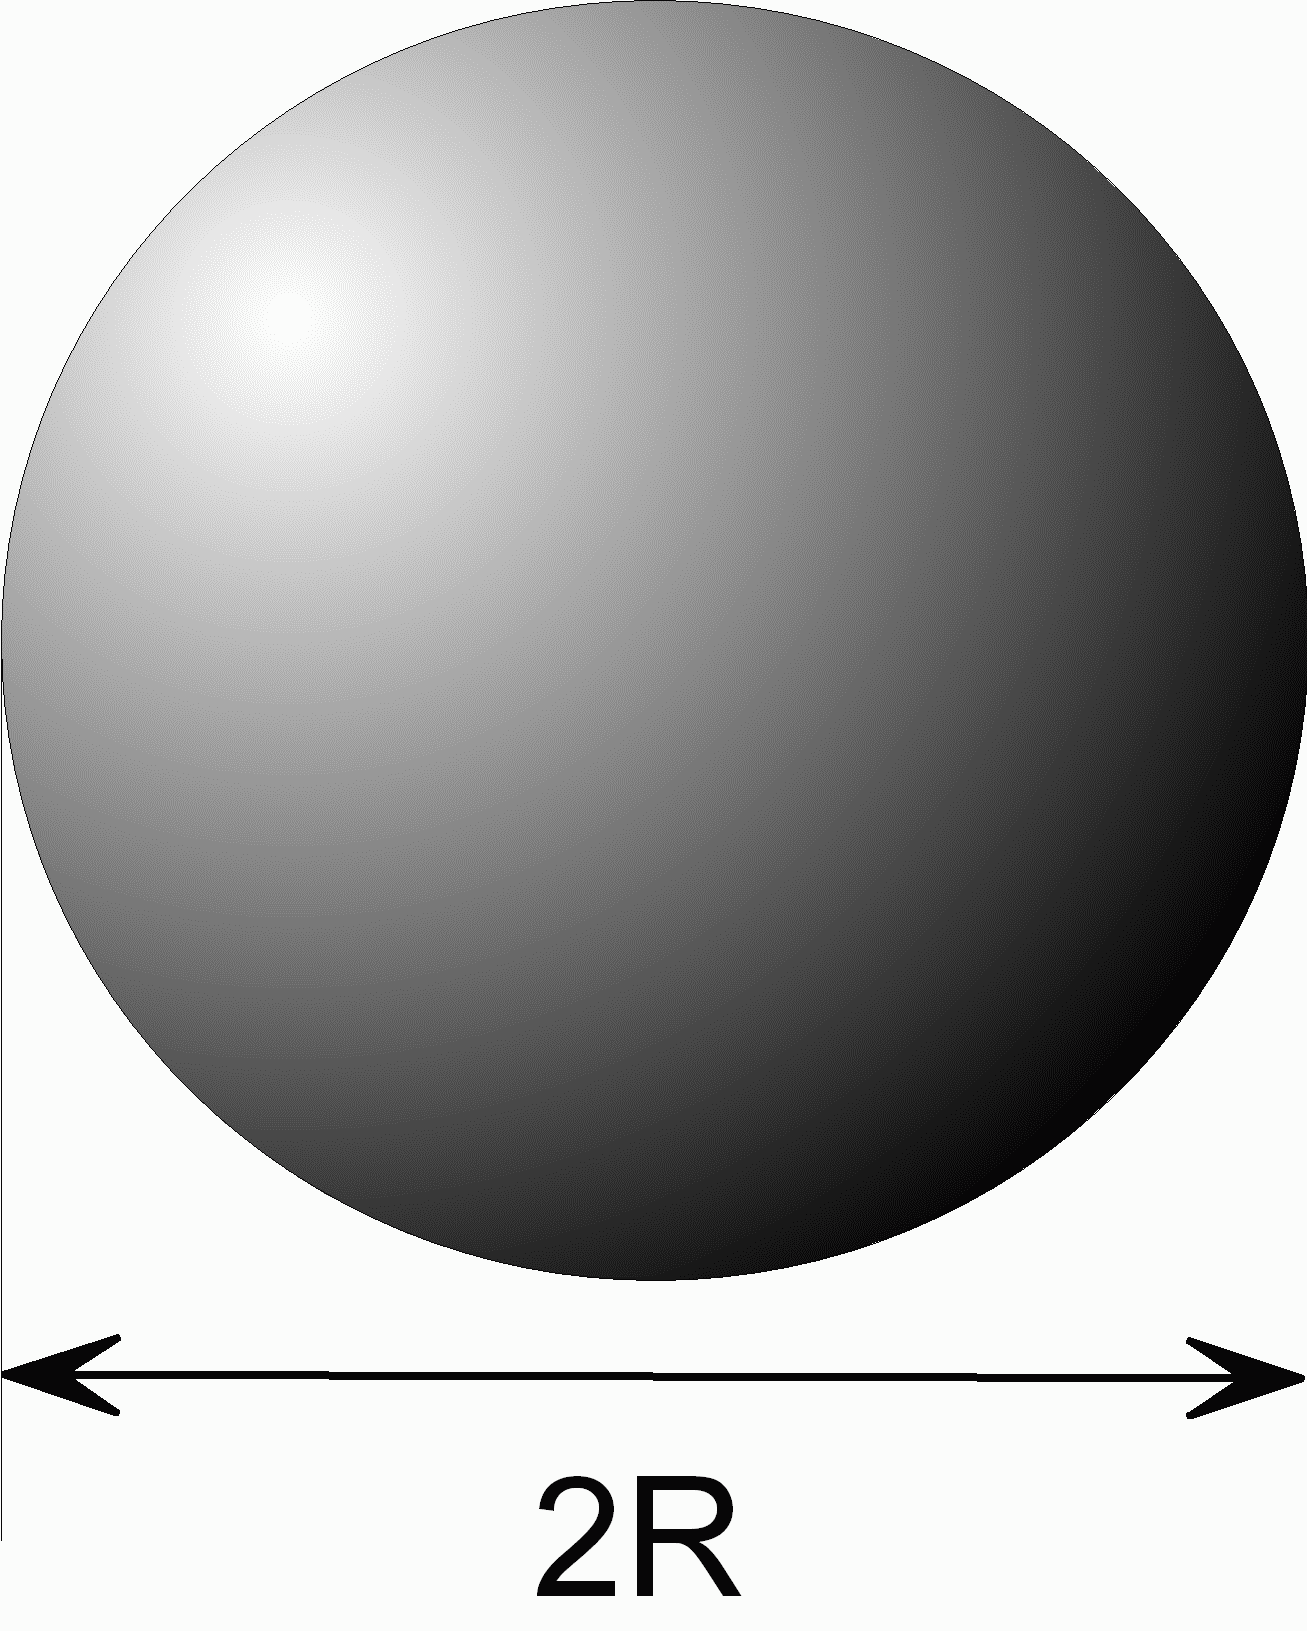
\includegraphics[width=0.2875\textwidth,height=0.359\textwidth]{../images/form_factor/spheres/sphere.png}
\end{center}
\caption{Sphere with diameter $2R$} \label{fig:Sketch_sphere}
\end{figure}

\begin{subequations}
\begin{align}
I_\text{Sphere}(Q,R) = K^2(Q,R,\Delta\eta) \label{eq:I_sphere}
\end{align}
with
\begin{align}
 K(Q,R,\Delta\eta) = \frac{4}{3}\pi R^3 \Delta\eta \, 3 \frac{\sin QR - QR \cos QR}{(QR)^3}
\end{align}
The forward scattering for $Q=0$ is given by
$$
\lim_{Q=0}I_\text{Sphere}(Q,R) =\left( \frac{4}{3}\pi R^3 \Delta\eta \right)^2
$$
\end{subequations}

\vspace{5mm}
\noindent \underline{Input Parameters for model \texttt{Sphere}:}
\begin{description}
\item[\texttt{R}] radius of sphere $R$
\item[- - -] not used
\item[- - -] not used
\item[\texttt{eta}] scattering length density difference between particle and matrix $\Delta\eta$
\end{description}

\noindent\underline{Note:}
\begin{itemize}
\item The parameters \texttt{param.p[1]} and \texttt{param.p[2]} are not used.
\end{itemize}

\begin{figure}[htb]
\begin{center}
\includegraphics[width=0.768\textwidth,height=0.588\textwidth]{../images/form_factor/spheres/sphere_P.png}
\end{center}
\caption{Scattering intensity of spheres with radii $R=10$nm and $R=20$nm.
The scattering length density contrast is set to 1.} \label{fig:I_sphere}
\end{figure}

%%%%%%%%%%%%%%%%%%%%%%%%%%%%%%%%%%%%%%%%%%%%%%%%%%%%%%%%%%
\clearpage

\subsection{Spherical Shell i}
\label{sect:spherical_shell_i} ~\\

\begin{figure}[htb]
\begin{center}
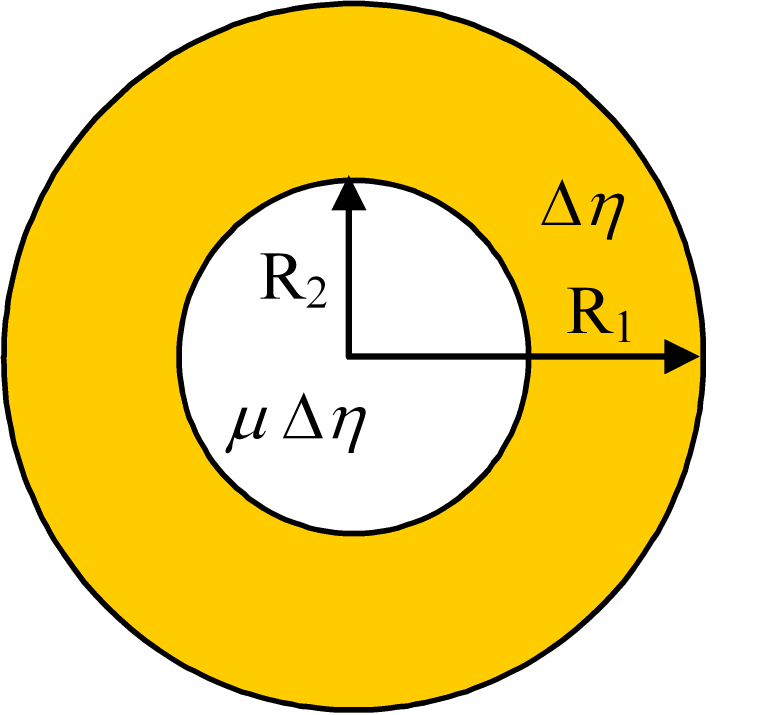
\includegraphics[width=0.38\textwidth,height=0.3575\textwidth]{../images/form_factor/spheres/shell1.png}
\end{center}
\caption{Spherical Shell i} \label{fig:shell1}
\end{figure}

This implementation of a spherical shell is parametrised with an inner radius $ R_2$ and outer
radius $R_1$. The scattering contrast relative to the matrix of the core is $\mu \Delta \eta$
and the one of the shell $\Delta\eta$.

\begin{align}
I_\text{Shell1}(Q,R_1,R_2,\Delta\eta,\mu)=
\left[K(Q,R_1,\Delta\eta)-K(Q,R_2,\Delta\eta(1-\mu))\right]^2
\end{align}
with
\begin{align}
 K(Q,R,\Delta\eta) = \frac{4}{3}\pi R^3 \Delta\eta \, 3 \frac{\sin QR - QR \cos QR}{(QR)^3}
\end{align}
The forward scattering for $Q=0$ is given by
$$
\lim_{Q=0}I_\text{Shell1}(Q,R_1,R_2,\Delta\eta,\mu) =
\left(\frac{4}{3}\pi \Delta\eta \left[ R_1^3 -
R_2^3(1-\mu)\right]\right)^2
$$

\vspace{5mm}
\noindent  \underline{Input Parameters for model \texttt{Spherical Shell i}:}
\begin{description}
\item[\texttt{R1}] overall radius of spherical shell $R_1$
\item[\texttt{R2}] radius of core $R_2$
\item[\texttt{eta}] scattering length density difference between shell and matrix $\Delta\eta$
\item[\texttt{mu}] scattering length density difference between core and matrix relative to the shell contrast $\mu$
\end{description}

\noindent\underline{Note:}
\begin{itemize}
\item[~] None
\end{itemize}

\begin{figure}[htb]
\begin{center}
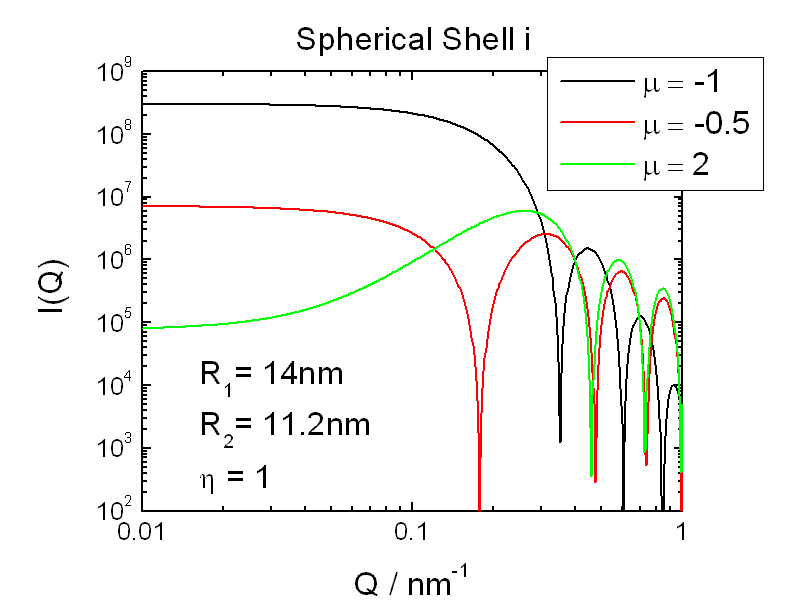
\includegraphics[width=0.768\textwidth,height=0.588\textwidth]{../images/form_factor/spheres/shell_i_P.png}
\end{center}
\caption{Scattering intensity of spherical shell with outer radius of $R_1=14$nm
and inner radius of $R_2=11.2$nm. The scattering length density contrast the shell is set to 1
and the one of the core to -1, -0.5, and 2.} \label{fig:I_shell_i}
\end{figure}


%%%%%%%%%%%%%%%%%%%%%%%%%%%%%%%%%%%%%%%%%%%%%%%%%%%%%%%%%%%
\clearpage
\subsection{Spherical Shell ii}
\label{sect:spherical_shell_ii} ~\\

\begin{figure}[htb]
\begin{center}
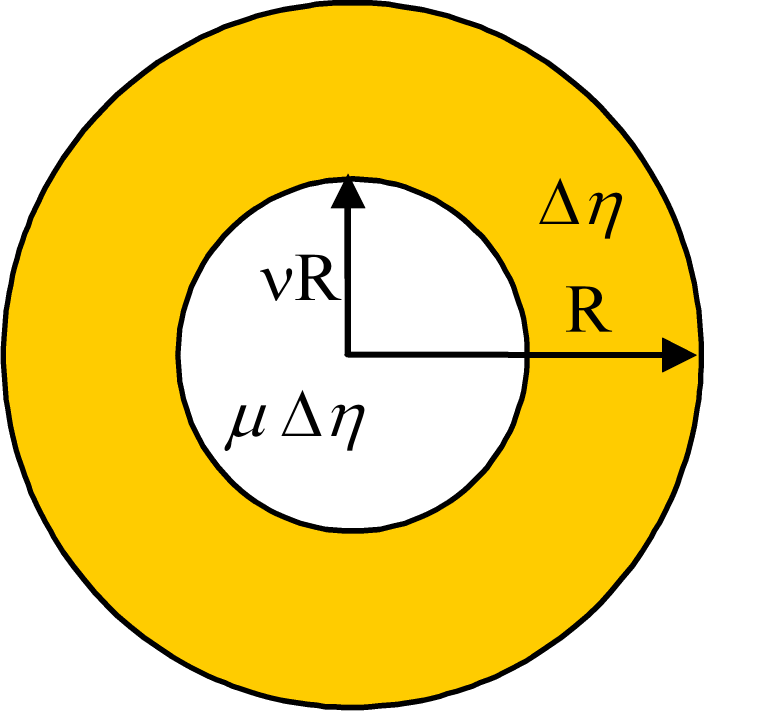
\includegraphics[width=0.38\textwidth,height=0.3575\textwidth]{../images/form_factor/spheres/shell2.png}
\end{center}
\caption{\texttt{Spherical Shell ii}} \label{fig:shell2}
\end{figure}
This implementation of a spherical shell is parametrised with an outer radius $R$ and an inner
radius $\nu R$. The scattering contrast relative to the matrix of the core is $ \mu \Delta \eta$
and the one of the shell $\Delta\eta$.
\begin{align}
I_\text{Shell2}(Q,R,\nu,\Delta\eta,\mu)=
\left(K(Q,R,\Delta\eta)-K(Q,\nu R,\Delta\eta(1-\mu))\right)^2
\end{align}
with
\begin{align}
 K(Q,R,\Delta\eta) = \frac{4}{3}\pi R^3 \Delta\eta \, 3 \frac{\sin QR - QR \cos QR}{(QR)^3}
\end{align}
The forward scattering for $Q=0$ is given by
$$
\DS \lim_{Q=0}I_\text{Shell2}(Q,R,R,\Delta\eta,\mu) =
\left(\frac{4}{3}\pi \Delta\eta \left[ R^3 - \nu^3
R^3(1-\mu)\right]\right)^2
$$

\vspace{5mm}
\noindent \underline{Input Parameters for model \texttt{Spherical Shell ii}:}
\begin{description}
\item[\texttt{R}] overall radius of spherical shell $R$
\item[\texttt{nu}] the radius of the core is only the fraction $\nu$ of the overall radius  $R$
\item[\texttt{eta}] scattering length density difference between shell and matrix $\Delta\eta$
\item[\texttt{mu}] scattering length density difference between core and matrix relative to the shell contrast $\mu$
\end{description}

\noindent\underline{Note:}
\begin{itemize}
\item[~] None
\end{itemize}

\begin{figure}[htb]
\begin{center}
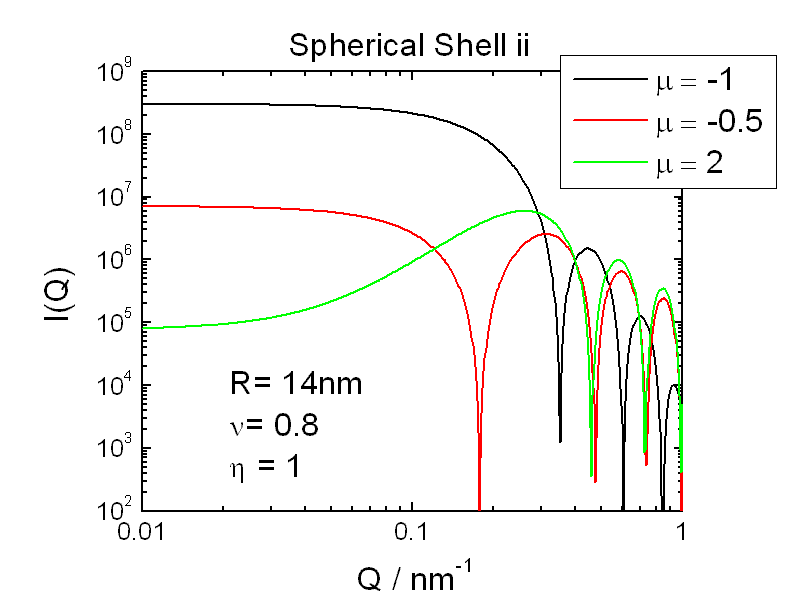
\includegraphics[width=0.768\textwidth,height=0.588\textwidth]{../images/form_factor/spheres/shell_ii_P.png}
\end{center}
\caption{Scattering intensity of spherical shell with outer radius of $R=14$nm
and inner radius of $\nu R=11.2$nm. The scattering length density contrast the shell is set to 1
and the one of the core to -1, -0.5, and 2.} \label{fig:I_shell_ii}
\end{figure}

%%%%%%%%%%%%%%%%%%%%%%%%%%%%%%%%%%%%%%%%%%%%%%%%%%%%%%%%%%%%%%%
\clearpage
\subsection{Spherical Shell iii}
\label{sect:spherical_shell_iii} ~\\

\begin{figure}[htb]
\begin{center}
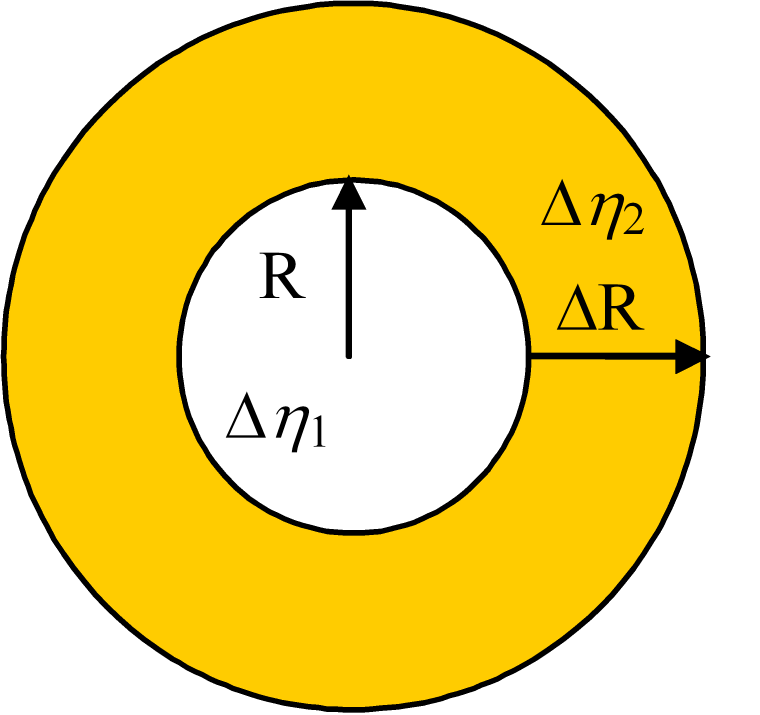
\includegraphics[width=0.38\textwidth,height=0.3575\textwidth]{../images/form_factor/spheres/shell3.png}
\end{center}
\caption{Spherical Shell iii} \label{fig:shell3}
\end{figure}
This implementation of a spherical shell is parametrised with an inner radius $R$ and a shell
thickness $\Delta R$. The scattering contrast relative to the matrix of the core is $ \Delta \eta_1$
and the one of the shell $\Delta\eta_2$.
\begin{align}
I_\text{Shell3}(Q,R,\Delta R,\Delta\eta_1,\Delta\eta_2)=
\left[K(Q,R+\Delta
R,\Delta\eta_2)-K(Q,R,\Delta\eta_2-\Delta\eta_1)\right]^2
\end{align}
with
\begin{align}
 K(Q,R,\Delta\eta) = \frac{4}{3}\pi R^3 \Delta\eta \, 3 \frac{\sin QR - QR \cos QR}{(QR)^3}
\end{align}
The forward scattering for $Q=0$ is given by
$$
\DS \lim_{Q=0}I_\text{Shell3}(Q,R,\Delta R,\Delta\eta_1,\Delta\eta_2)
= \left(\frac{4}{3}\pi \left[(R+\Delta R)^3\Delta\eta_2
                            - R^3(\Delta\eta_2-\Delta\eta_1)\right]\right)^2
$$

\vspace{5mm}
\noindent  \underline{Input Parameters for model \texttt{Spherical Shell iii}:}
\begin{description}
\item[\texttt{R}] radius of core $R$
\item[\texttt{dR}] thickness of the shell $\Delta R$
\item[\texttt{eta1}] scattering length density difference between core and matrix $\Delta\eta_1$
\item[\texttt{eta2}] scattering length density difference between shell and matrix $\Delta\eta_2$
\end{description}

\noindent\underline{Note:}
\begin{itemize}
\item[~] None
\end{itemize}


\begin{figure}[htb]
\begin{center}
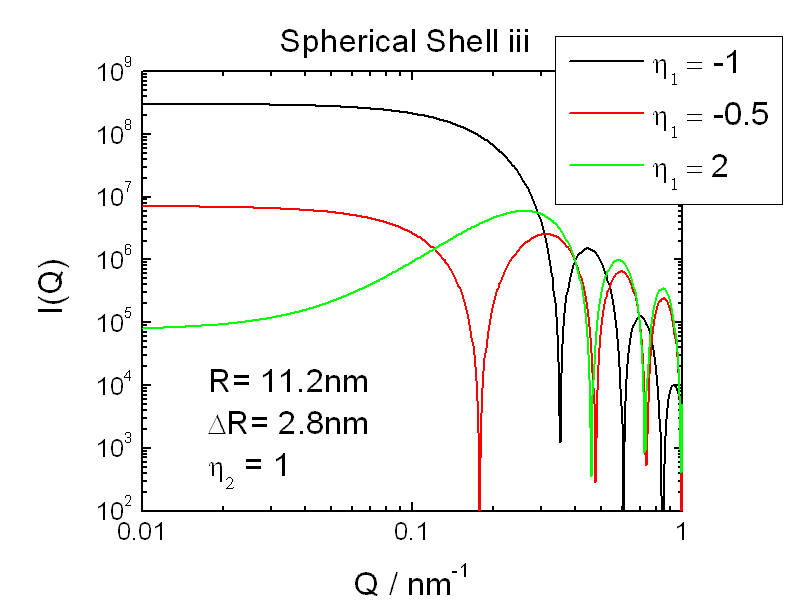
\includegraphics[width=0.768\textwidth,height=0.588\textwidth]{../images/form_factor/spheres/shell_iii_P.png}
\end{center}
\caption{Scattering intensity of spherical shell with core radius of $R=11.2$nm
and shell thickness of $\Delta R=2.8$nm. The scattering length density contrast the shell is set to 1
and the one of the core to -1, -0.5, and 2.} \label{fig:I_shell_iii}
\end{figure}
\clearpage


%%%%%%%%%%%%%%%%%%%%%%%%%%%%%%%%%%%%%%%%%%%%%%%%%%%%%%%%%%%%%%%%%%%%%%%%%%

\clearpage
\subsection{Bilayered Vesicle}
\label{sect:BilayeredVesicle} ~\\

\begin{figure}[htb]
\begin{center}
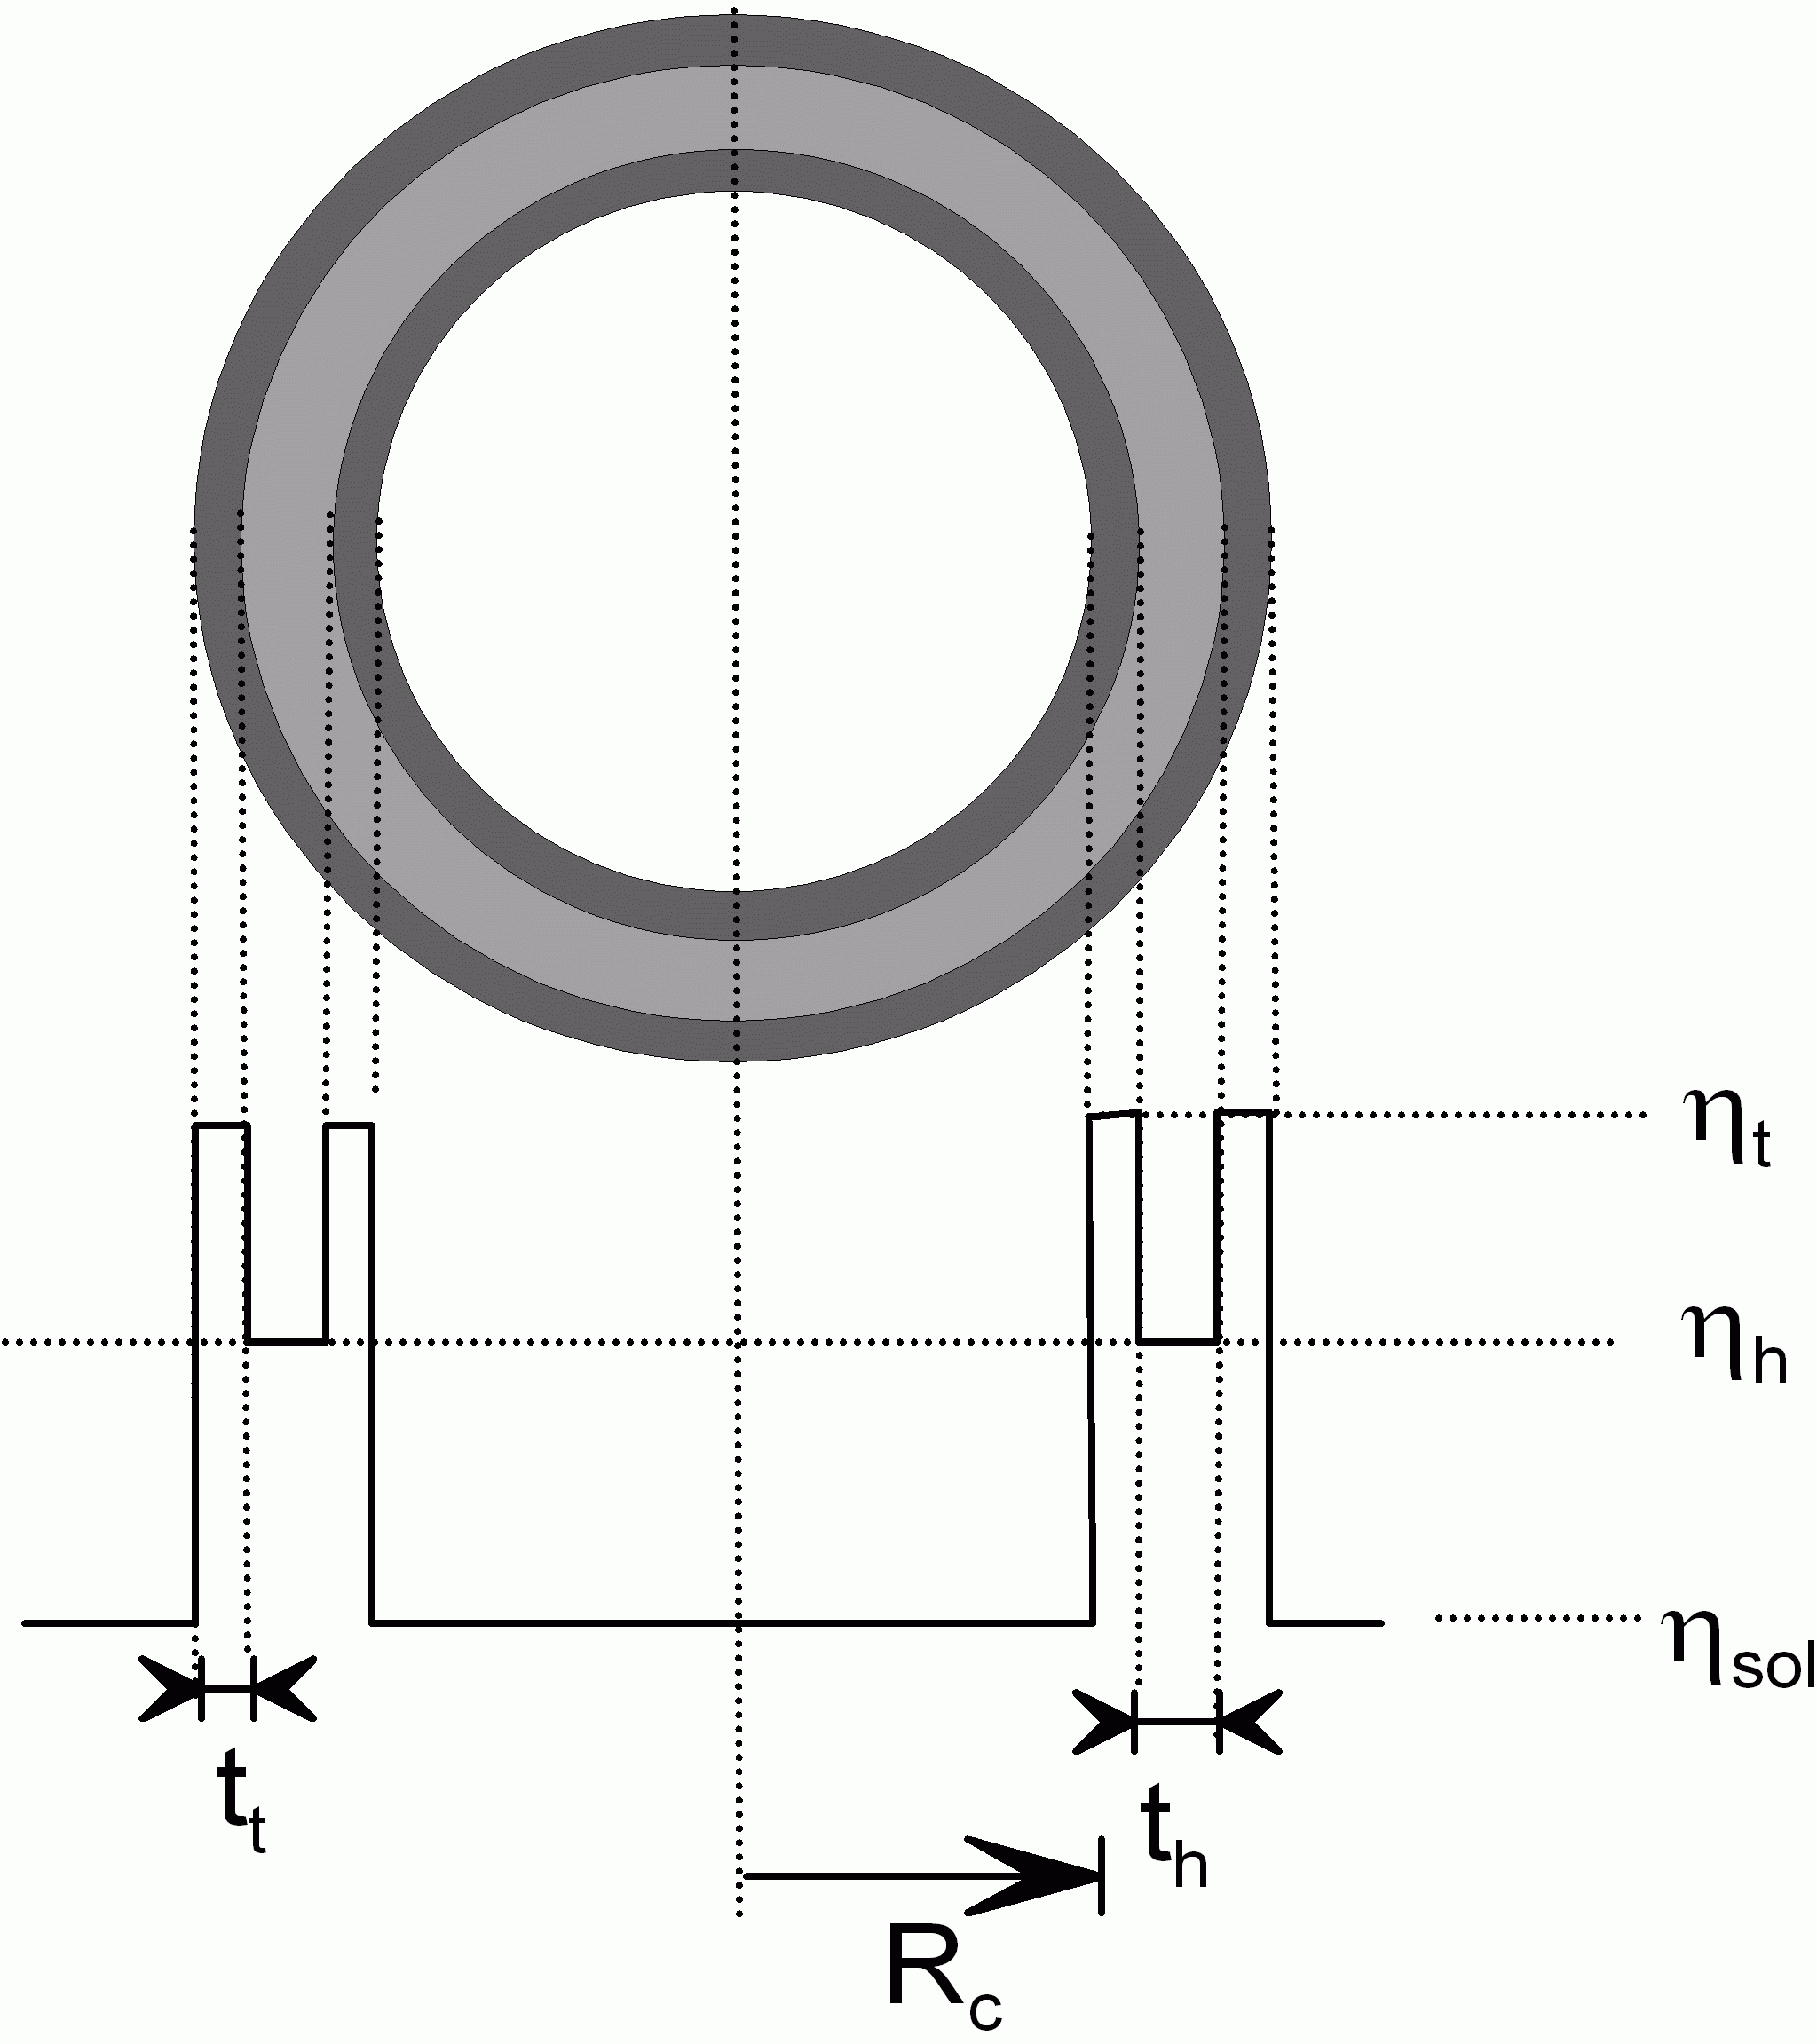
\includegraphics[width=0.5441\textwidth,height=0.5858\textwidth]{../images/form_factor/spheres/BiLayeredVesicle.png}
\end{center}
\caption{BiLayeredVesicle} \label{fig:BiLayeredVesicle}
\end{figure}
\begin{align}
I_\text{BLV}(Q) = \bigg( & + K(Q,R_c,\eta_{sol}-\eta_{t})+ K(Q,R_c+t_{t},\eta_{t}-\eta_{h}) \\
&+ K(Q,R_c+t_{t}+t_{h},\eta_{h}-\eta_{t}) +
K(Q,R_c+2t_{t}+t_{h},\eta_{t}-\eta_{sol}) \bigg)^2 \nonumber
\end{align}
with
\begin{align}
 K(Q,R,\Delta\eta) = \frac{4}{3}\pi R^3 \Delta\eta \, 3 \frac{\sin QR - QR \cos QR}{(QR)^3}
\end{align}

\vspace{5mm}
\hspace{1pt}\\
\underline{Input Parameters for model \texttt{BilayeredVesicle}:}\\
\begin{description}
\item[\texttt{R\_c}] radius of core $R_c$ which consists of solvent
\item[\texttt{t\_h}] thickness of outer part of bilayer (in contact with solvent, head group) $t_\text{h}$
\item[\texttt{t\_t}] thickness of inner part of bilayer (tail group) $t_\text{t}$
\item[\texttt{eta\_sol}] scattering length density of solvent $\eta_\text{sol}$
\item[\texttt{eta\_h}] scattering length density of outer part of bilayer $\eta_\text{h}$
\item[\texttt{eta\_t}] scattering length density of inner part of bilayer $\eta_\text{t}$
\end{description}

\noindent\underline{Note:}
\begin{itemize}
\item[~] None
\end{itemize}

\begin{figure}[htb]
\begin{center}
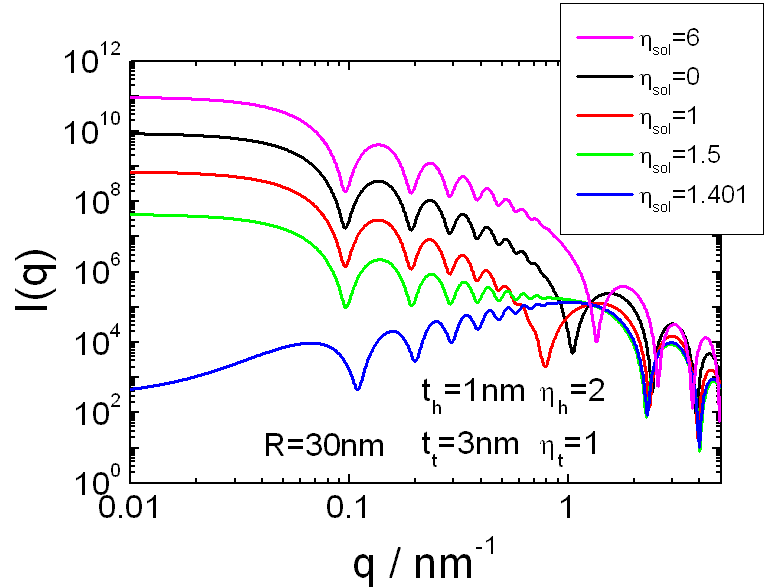
\includegraphics[width=0.768\textwidth,height=0.588\textwidth]{../images/form_factor/spheres/bilayered_vesicle.png}
\end{center}
\caption{Scattering intensity of a bilayered vesicle. The scattering intensity has been calculated
with a lognormal $[\mathrm{LogNorm}(N\!=\!1,\sigma\!=\!0.05,p\!=\!1,R\!=\!30)]$ size distribution for the vesicle radius $R_c$.}
\label{fig:I_BiLayeredVesicle}
\end{figure}

%%%%%%%%%%%%%%%%%%%%%%%%%%%%%%%%%%%%%%%%%%%%%%%%%%%%%%%%%%%%%%%%%%

\clearpage
\subsection{Multi Lamellar Vesicle}
\label{sect:MultiLamellarVesicle} ~\\

\begin{figure}[htb]
\begin{center}
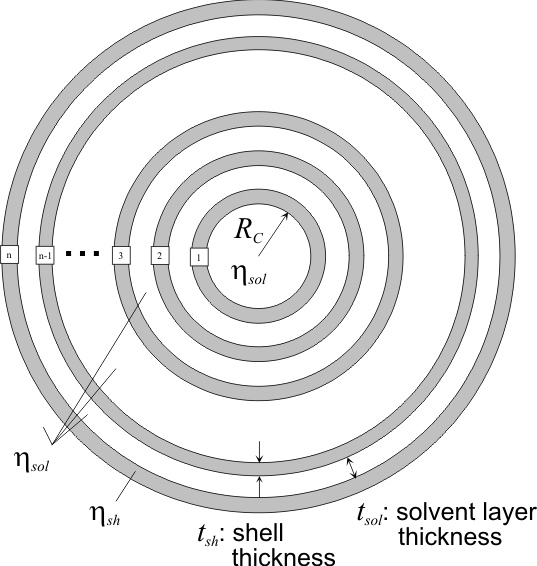
\includegraphics[width=0.537\textwidth,height=0.566\textwidth]{../images/form_factor/spheres/multilamellar_vesicle.png}
\end{center}
\caption{MultiLamellarVesicle} \label{fig:MultiLamellarVesicle}
\end{figure}
\begin{align}
I_\text{MLV}(Q) = \Bigg( \sum_{i=0}^{n-1} \bigg[ & K(Q,R_c+it_{sh}+it_{sol},\eta_{sol}-\eta_{sh}) \nonumber \\
+ &K(Q,R_c+(i+1)t_{sh}+it_{sol},\eta_{sh}-\eta_{sol}) \bigg]
\Bigg)^2
\end{align}
with
\begin{align}
 K(Q,R,\Delta\eta) = \frac{4}{3}\pi R^3 \Delta\eta \, 3 \frac{\sin QR - QR \cos QR}{(QR)^3}
\end{align}


\noindent\underline{Input Parameters for model \texttt{MultiLamellarVesicle}:}
\begin{description}
\item[\texttt{R\_c}] radius of core $R_c$ which consists of solvent
\item[\texttt{t\_sh}] surfactant layer thickness $t_\text{sh}$
\item[\texttt{t\_sol}] thickness of solvent layer $t_\text{sol}$
\item[\texttt{eta\_sh}] scattering length density of surfactant layer $\eta_\text{sh}$
\item[\texttt{eta\_sol}] scattering length density of solvent $\eta_\text{sol}$
\item[\texttt{n}] total number of surfactant layers $n$
\end{description}

\noindent\underline{Note:}
\begin{itemize}
\item[~] None
\end{itemize}


\begin{figure}[htb]
\begin{center}
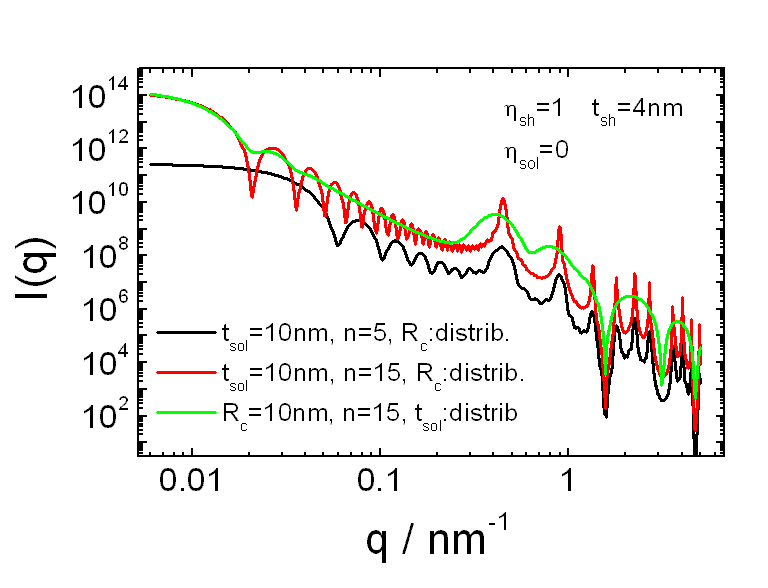
\includegraphics[width=0.768\textwidth,height=0.588\textwidth]{../images/form_factor/spheres/multilamellar_vesicle_Iq.png}
\end{center}
\caption{Scattering intensity of a multilamellar vesicle. The scattering intensities has been calculated
for a\&b) a distribution of the core radius $R_c$ by
$\int\mathrm{LogNorm}(R_c;N\!=\!1,\sigma\!=\!0.3,p\!=\!1,R\!=\!10) I(q,R_c)\, \mathrm{d}R_c$
and c) for a distribution of the distances between the lamellars
$\int\mathrm{LogNorm}(t_\text{sol};N\!=\!1,\sigma\!=\!0.3,p\!=\!1,R\!=\!10) I(q,t_\text{sol})\, \mathrm{d}t_\text{sol}$.}
\label{fig:I_MLV}
\end{figure}

%%%%%%%%%%%%%%%%%%%%%%%%%%%%%%%%%%%%%%%%%%%%%%%%%%%%%%%%%%%%%%%%%%

\clearpage
\subsection{RNDMultiLamellarVesicle}
\label{sect:MultiLamellarVesicle} ~\\

\begin{figure}[htb]
\begin{center}
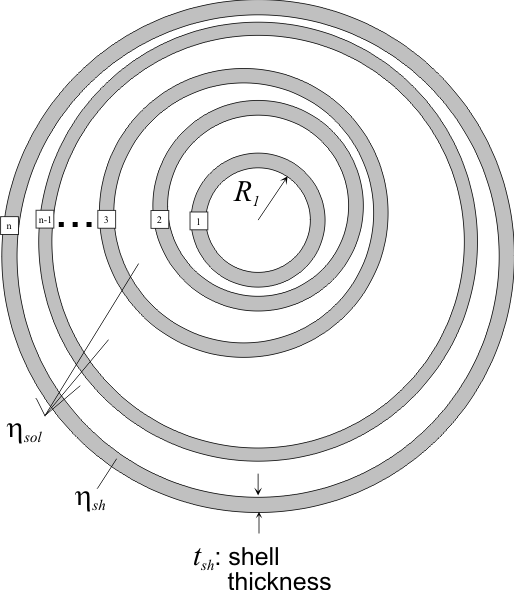
\includegraphics[width=0.537\textwidth,height=0.566\textwidth]{../images/form_factor/spheres/random_multilamellar_vesicle.png}
\end{center}
\caption{randomMultiLamellarVesicle}
\label{fig:randomMultiLamellarVesicle}
\end{figure}
\begin{align}
I_\text{RndMLV}(Q) &= \Delta\eta ^2 \sum_{i=1}^{N} F_i^2(q,R_i,t_{sh,i}) \nonumber \\
&+ \Delta\eta ^2 \sum_{i<j}^{N} 2 F_i(q,R_i,t_{sh,i}) F_j(q,R_j,t_{sh,j}) \frac{\sin qr_{ij}}{qr_{ij}}
\end{align}
with
\begin{subequations}
\begin{align}
r_{ij} & = \abs{\mathbf{R}_i-\mathbf{R}_j} \\
F_i(q,R_i,t_{sol,i}) &= K(q,R_i+t_{sol,i},\Delta\eta)-K(q,R_i,\Delta\eta)\\
K(q,R,\Delta\eta) &= \frac{4}{3}\pi R^3 \Delta\eta \, 3 \frac{\sin qR - qR \cos qR}{(qR)^3}
\end{align}
\end{subequations}

\begin{subequations}
\begin{align}
R_1 &= \textrm{ran}_{lognormal}\left(\log(R_c),\sigma_{R_c}\right) \\
\Delta R_{i} &= \textrm{ran}_{gaussian}\left(\sigma_{t_{sol}}\right) \\
R_i &= R_{i-1}+t_{sh,i-1}+\Delta R_{i}\\
\mathbf{R}_i &= R_i \; \textbf{ran}_{dir,3D}
                       \text{ran}_{uniform} \; \Delta t_{sol}
\end{align}
\end{subequations}


\hspace{1mm}\\
\underline{Input Parameters for model
\texttt{RNDMultiLamellarVesicle}:}
\begin{description}
\item[\texttt{t\_sh}] average surfactant layer thickness $t_\text{sh}$
\item[\texttt{s\_sh}] Gaussian thickness distribution of surfactant layer with a width of $\sigma_\text{sh}$
\item[\texttt{R\_c}] average radius of core $R_c$ which consists of solvent
\item[\texttt{s\_c}] lognormal size distribution of core radius $R_c$ with a width of $\sigma_c$
\item[\texttt{n}] average number of surfactant layers $n$
\item[\texttt{s\_n}] lognormal distribution of the number of surfactant layers with a width of $\sigma_n$
\item[\texttt{t\_sol}] average thickness of solvent layer $t_\text{sol}$
\item[\texttt{s\_sol}] lognormal thickness distribution of solvent layer with a width of $\sigma_\text{sol}$
\item[\texttt{Deta\_sh}] scattering length density contrast $\Delta\eta$ between surfactant layer and solvent
\end{description}

\noindent\underline{Note:}
\begin{itemize}
\item[~] The number of Monte Carlo iterations can be set via the menu \texttt{[Options|Customize...]}
\end{itemize}

\begin{figure}[htb]
\begin{center}
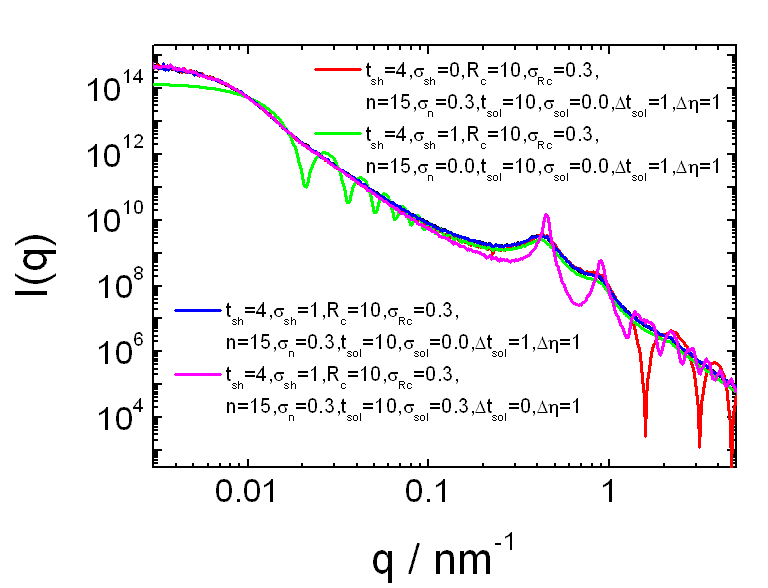
\includegraphics[width=0.768\textwidth,height=0.588\textwidth]{../images/form_factor/spheres/random_multilamellar_vesicle_Iq.png}
\end{center}
\caption{Scattering intensity of a multilamellar vesicle where several distribution of parameters
within a single vesicle are calculated via a Monte Carlo algorithm. .}
\label{fig:I_rndMLV}
\end{figure}
%%%%%%%%%%%%%%%%%%%%%%%%%%%%%%%%%%%%%%%%%%%%%%%%%%%%%%%%%%%%%%%%%%

\clearpage
\subsection{Vesicle with aligned flat capped ends \cite{Kaya:aj5008,Kaya:aj5016}}
\label{sect:vesicle_capped_poles_aligned} ~\\

\begin{figure}[htb]
\begin{center}
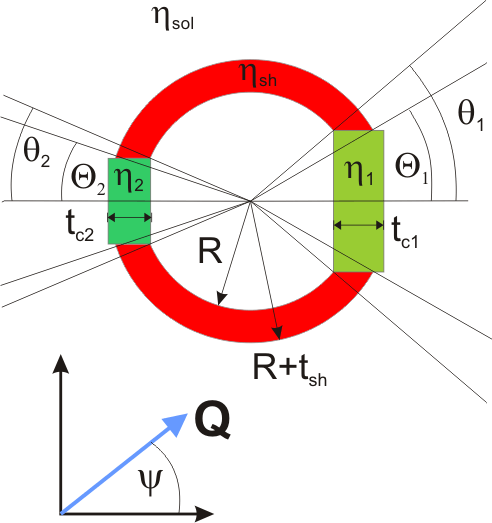
\includegraphics[width=0.492\textwidth,height=0.523\textwidth]{vesicle_capped_poles_aligned.png}
\end{center}
\caption{Sketch of a vesicle with horizontally aligned flat
capped ends perpendicular to the incoming neutron beam}
\label{fig:Sketch_vesicle_capped_poles_aligned}
\end{figure}
The shape of this form factor consist of spherical vesicle containing to flat domains.
The flat thought to be aligned in a horizontal magnetic field perpendicular to the incoming
neutron beam. The size of the domains are characterized by the angles $\theta_1$ and
$theta_2$. The thicknesses $t_{c1}$ and $t_{c2}$ can be different than the thickness $t_{sh}$
of the spherical part of the vesicles. The same hold for the scattering length densities
$\eta_{c1}$, $\eta_{c2}$ and $\eta_{sh}$. The form factor $F_\text{cv}(Q)$ of this object can be
calculated by performing the Fourier transformation of the scattering length density in separate
steps. First one calculates the Fourier transformation of a sphere $F_\text{cSph}$
with flat capped ends on each side in cylinder coordinates.
\begin{subequations}
\begin{align}
F_\text{cSph}(Q,R,\psi,\theta_1,\theta_2,\Delta\eta) = \Delta\eta \!\!
\int_{-R\cos\theta_2}^{R\cos\theta_1} \!\!\!\!\! \mathrm{d}z \!\!\!
\int_0^{\sqrt{R^2-z^2}}\!\!\!\!\! \mathrm{d}\rho \;
\int_0^{2\pi} \mathrm{d}\phi \;\; e^{\imath \mathbf{Q}\cdot\mathbf{r}}
\, \rho
\label{eq:FcSphInt}
\end{align}
\begin{align}
\text{with} \quad
\mathbf{Q}=Q\left(
              \begin{array}{c}
                0 \\
                \sin\psi \\
                \cos\psi
              \end{array}
            \right)
\quad \text{and} \quad
\mathbf{r}= \left(
              \begin{array}{c}
                \rho \cos\phi \\
                \rho \sin\phi \\
                z
              \end{array}
            \right)
\end{align}
\end{subequations}
The form factor of vesicle $F_\text{cv}(Q)$ with a layer thickness of $t_\text{sh}$ can than
be calculated by
\begin{subequations}
\begin{align}
F_\text{cv}(Q,R,t_\text{sh},\theta_1,\theta_2,\Delta\eta_\text{sh}) =
    & + F_\text{cSph}(Q,R+t_\text{sh},\Theta_1,\Theta_2,\Delta\eta_\text{sh}) \nonumber \\
    & - F_\text{cSph}(Q,R,            \theta_1,\theta_2,\Delta\eta_\text{sh})
\end{align}
with
\begin{align}
\Theta_1 &= \arcsin\left(\frac{R_{c1}}{R+t_\text{sh}} \right), \quad R_{c1} = R \sin\left(\theta_1\right),\\
\Theta_2 &= \arcsin\left(\frac{R_{c2}}{R+t_\text{sh}} \right), \quad R_{c2} = R \sin\left(\theta_2\right).
\end{align}
\end{subequations}
As the flat capped ends are allowed to have independent thicknesses $t_\text{c1}$, $t_\text{c2}$ and
scattering length densities $\eta_\text{1}$, $\eta_\text{2}$ the scattering amplitude contribution of the
flat capped ends, which have the shape of a disc, need to be corrected. Their contribution can be calculated by
\newlength\breite
\settowidth\breite{$\displaystyle {}+{}$}
\begin{multline}
\begin{split}
F_\text{c}(Q,R,\theta_1,\theta_2,\dots) =
& \hspace{\breite} F_\text{c1}(Q,R,\theta_1,\Delta\eta_\text{c1}) - F_\text{d1}(Q,R,t_\text{d1},\Delta\eta_\text{sh}) \\
& +                F_\text{c2}(Q,R,\theta_2,\Delta\eta_\text{c2}) - F_\text{d2}(Q,R,t_\text{d2},\Delta\eta_\text{sh})
\end{split} \\[2mm]
\begin{split}
= & \hspace{\breite} \Delta\eta_\text{c1} \!\!\!
\int_{l_\text{c1}}^{l_\text{c1}+t_\text{c1}} \!\!\!\!\!
\mathrm{d}z\int_0^{R_\text{c1}} \!\!  \mathrm{d}\rho \int_0^{2\pi}\!\! \mathrm{d}\phi \; e^{\imath \mathbf{Q}\cdot\mathbf{r}}
\, \rho
- \Delta\eta_\text{sh} \!\!\!
\int_{l_\text{c1}}^{l_\text{c1}+t_\text{d1}} \!\!\!\!\!
\mathrm{d}z\int_0^{R_\text{c1}} \!\! \mathrm{d}\rho \int_0^{2\pi}\!\! \mathrm{d}\phi \; e^{\imath \mathbf{Q}\cdot\mathbf{r}}
\, \rho  \\
& + \Delta\eta_\text{c2} \!\!\!\!\!\!\!
\int_{-(l_\text{c2}+t_\text{c2})}^{-l_\text{c2}} \!\!\!\!\!\!\!\!
\mathrm{d}z\int_0^{R_\text{c2}} \!\! \mathrm{d}\rho \int_0^{2\pi}\!\!\mathrm{d}\phi \; e^{\imath \mathbf{Q}\cdot\mathbf{r}}
\, \rho
- \Delta\eta_\text{sh} \!\!\!\!\!\!\!
\int_{-(l_\text{c2}+t_\text{d2})}^{-l_\text{c2}} \!\!\!\!\!\!\!\!
\mathrm{d}z\int_0^{R_\text{c2}} \!\! \mathrm{d}\rho  \int_0^{2\pi}\!\!\mathrm{d}\phi \; e^{\imath \mathbf{Q}\cdot\mathbf{r}}
\, \rho \label{eq:Fc}
\end{split}
\end{multline}
with
\begin{subequations}
\begin{align}
\Delta\eta_\text{sh} &= \eta_\text{sh}-\eta_\text{sol}, \, \Delta\eta_\text{c1} = \eta_1-\eta_\text{sol} , \,
\Delta\eta_\text{c2} = \eta_2-\eta_\text{sol} \\
l_\text{c1} &= R\cos{\theta_1}, \, l_\text{c2} = R\cos{\theta_2} \\
R_\text{c1} &= R\sin{\theta_1}, \, R_\text{c2} = R\sin{\theta_2} \\
t_\text{d1} &= \sqrt{\left(R+t_\text{sh}\right)^2-R_\text{c1}^2}-\sqrt{R^2-R_\text{c1}^2} \\
t_\text{d2} &= \sqrt{\left(R+t_\text{sh}\right)^2-R_\text{c2}^2}-\sqrt{R^2-R_\text{c2}^2} \\
\end{align}
\end{subequations}
The solution of the integrals in eq.\ \ref{eq:FcSphInt} and \ref{eq:Fc} are
\begin{subequations}
\begin{multline}
F_\text{cSph}(Q,R,\psi,\theta_1,\theta_2,\Delta\eta) = \Delta\eta \!\!
\int_{-R\cos\theta_2}^{R\cos\theta_1} \!\!\!\!\! \mathrm{d}z \!\!\!
\int_0^{\sqrt{R^2-z^2}}\!\!\!\!\! \mathrm{d}\rho \;
\int_0^{2\pi} \mathrm{d}\phi \;\; e^{\imath \mathbf{Q}\cdot\mathbf{r}}
\, \rho  \\
 \Delta\eta \!\!
\int_{-R\cos\theta_2}^{R\cos\theta_1} \!\!\!\!\! \mathrm{d}z\;\;
\exp\left(\imath Q z \cos\psi\right)  2\pi \left(R^2 - z^2\right)
\frac{J_1\left(Q \sqrt{R^2 - z^2} \sin\psi\right)}{Q \sqrt{R^2 - z^2} \sin\psi}
\label{eq:FcSphPsi}
\end{multline}
and
\begin{multline}
F_\textrm{c$_i$,d$_i$}(Q,R_\textrm{c$_i$,d$_i$},\psi,\Delta\eta)   =
\Delta\eta \int_{a}^{b}\!\! \mathrm{d}z
           \int_0^{R_\textrm{c$_i$}}\!\! \mathrm{d}\rho
           \int_0^{2\pi}\!\! \mathrm{d}\phi \;\; e^{\imath \mathbf{Q}\cdot\mathbf{r}}
\, \rho \\
 = 4 \pi R \frac{\imath \left(\exp\left(\imath a Q \cos\psi\right)-\exp\left(\imath b Q \cos\psi\right)\right)
 J_1\left(Q R \sin\psi\right)}{\sin\left(2\psi\right) Q^2}
\end{multline}
\end{subequations}
whereby $\mathrm{J}_1$ the regular cylindrical Bessel function of first order.
The overall scattering intensity $I_{\textrm{alignedVes}}(Q,\psi,\dots)$ is finally given by
\begin{align}
I_{\textrm{alignedVes}}(Q,\psi,\dots) =
\abs{
 F_\text{cv}(Q,R,\psi,t_\text{sh},\theta_1,\theta_2,\Delta\eta_\text{sh})
+F_\text{c}(Q,R,\psi,\theta_1,\theta_2,\dots)}^2
\end{align}
\vspace{5mm}
\begin{sloppypar}
\noindent \underline{Input Parameters for the models of \texttt{MagneticFieldAlignedVesicle}:}
\end{sloppypar}
\begin{description}
\item[\texttt{Rsh}] radius of spherical vesicle shell
\item[\texttt{theta1}] angle to describe size of first capped side
\item[\texttt{theta2}] angle to describe size of second capped side
\item[\texttt{t\_sh}] thickness of spherical vesicle shell
\item[\texttt{t\_c1}] thickness of first flat capped side
\item[\texttt{t\_c2}] thickness of second flat capped side
\item[\texttt{eta\_sh}] scattering length density of spherical vesicle shell
\item[\texttt{eta\_1}] scattering length density of first capped side
\item[\texttt{eta\_2}] scattering length density of second capped side
\item[\texttt{eta\_sol}] scattering length density of solvent
\end{description}

\noindent\underline{Note:}
\begin{itemize}
\item[~] None
\end{itemize}

\begin{figure}[htb]
\begin{center}
%\includegraphics[width=0.768\textwidth,height=0.588\textwidth]{sphere_P.png}
\end{center}
%\caption{Scattering intensity of spheres with radii $R=10$nm and $R=20$nm.
%The scattering length density contrast is set to 1.} \label{fig:I_sphere}
\end{figure}

%%%%%%%%%%%%%%%%%%%%%%%%%%%%%%%%%%%%%%%%%%%%%%%%%%%%%%%%%%%%%%%%%%%%%%%%%%%%%%%%

\clearpage
\subsection{Spherical shell with linear varying contrast profile (LinShell)}
\label{sect:LinShell} ~\\

\begin{figure}[htb]
\begin{center}
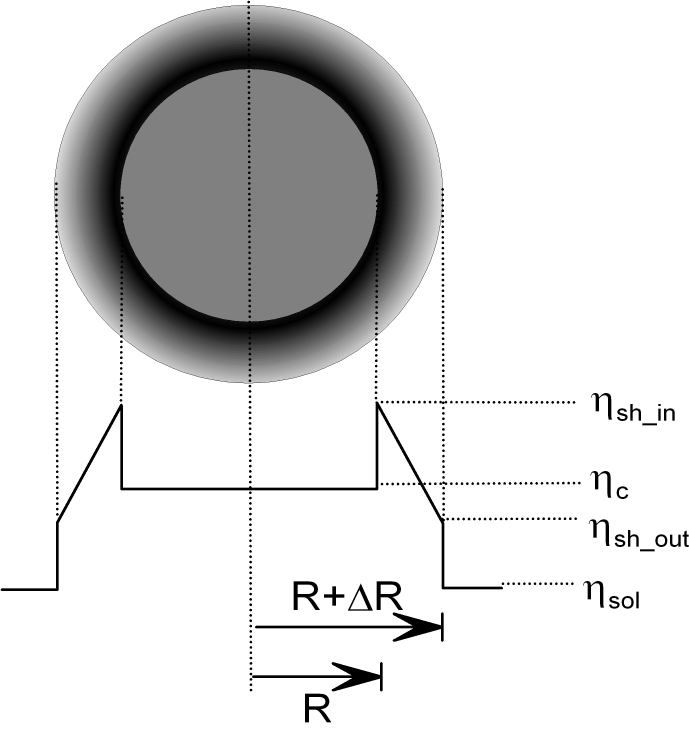
\includegraphics[width=0.5\textwidth,height=0.533\textwidth]{../images/form_factor/spheres/linshell.png}
\end{center}
\caption{Form factor of a spherical shell with a core radius $R$
and a shell thickness of $\Delta R$ and a linear varying contrast
profile.} \label{linshell}
\end{figure}

Form factor of a spherical shell with a core radius $R$ and a
shell thickness of $\Delta R$. Here a linear contrast profile
within the shell has been assumed.

\begin{align}
\Delta\eta(r)      & =
\begin{cases}
\eta_\text{c}-\eta_\text{sol} & \text{~for~} r<R \\
m r + b  & \text{~for~} r \in [R,R+\Delta R] \\
0  & \text{~for~} r>R+\Delta R
\end{cases}\\
m           & = (\eta_\text{sh\_out}-\eta_\text{sh\_in}) / \Delta R \\
b           & = -m R + \eta_\text{sh\_in} - \eta_\text{sol} \\
\eta_\text{sh\_in}  & = (1 - x_\text{in,sol})  \, \eta_\text{sh} + x_\text{in,sol} \,\eta_\text{sol}-\eta_\text{sol} \\
                    & : \text{scattering length density at $R$} \nonumber \\
\eta_\text{sh\_out} & = (1 - x_\text{out,sol}) \, \eta_\text{sh} + x_\text{out,sol}\,\eta_\text{sol}-\eta_\text{sol} \\
                    & : \text{scattering length density at $R+\Delta R$} \nonumber \\
\eta_\text{sh}      & : \text{scattering length density of pure shell material} \nonumber \\
\eta_\text{c}       & : \text{scattering length density of core} \nonumber \\
\nonumber
\end{align}

\begin{align}
F_\text{sph}(A,x) & = \frac{4}{3}\pi x^3 \,\, 3\frac{\sin(A)-A\cos(A)}{A^3} \\[5mm]
F_\text{shlin}(A,x) & = 4\pi x^4 \frac{2\cos(A)+2A\sin(A)-A^2\cos(A)}{A^4} \\[5mm]
I_\text{LinShell}    & = \big[ \,\, (\eta_\text{c}-\eta_\text{sol}-b)F_\text{sph}(QR,R) \nonumber \\
             & \hspace{6mm} - mF_\text{shlin}(QR,R) \\
             & \hspace{6mm} + mF_\text{shlin}\left(Q(R+\Delta R),R+\Delta R\right) \nonumber \\
             & \hspace{6mm} + bF_\text{sph}\left(Q(R+\Delta R),R+\Delta R\right) \big]^2 \nonumber
\end{align}

\vspace{5mm}

\underline{Input Parameters for model \texttt{LinShell}:}\\
\begin{description}
\item[\texttt{R}] radius of core $R$
\item[\texttt{dR}] thickness of the shell $\Delta R$
\item[\texttt{eta\_c}] scattering length density $\eta_\text{c}$
\item[\texttt{eta\_sh}] scattering length density of non-swollen shell $\eta_\text{sh}$
\item[\texttt{x\_in}] amount of solvent $x_\text{in,sol}$ on core-shell interface at $R$
\item[\texttt{x\_out}] amount of solvent $x_\text{out,sol}$ on shell-solvent interface at $R+\Delta R$
\item[\texttt{eta\_sol}] scattering length density of solvent $\eta_\text{sol}$
\end{description}

\noindent\underline{Note:}
\begin{itemize}
\item $x_\text{in,sol}$ and $x_\text{out,sol}$ are only physical for values between 0 and 1.
\end{itemize}


\begin{figure}[htb]
\begin{center}
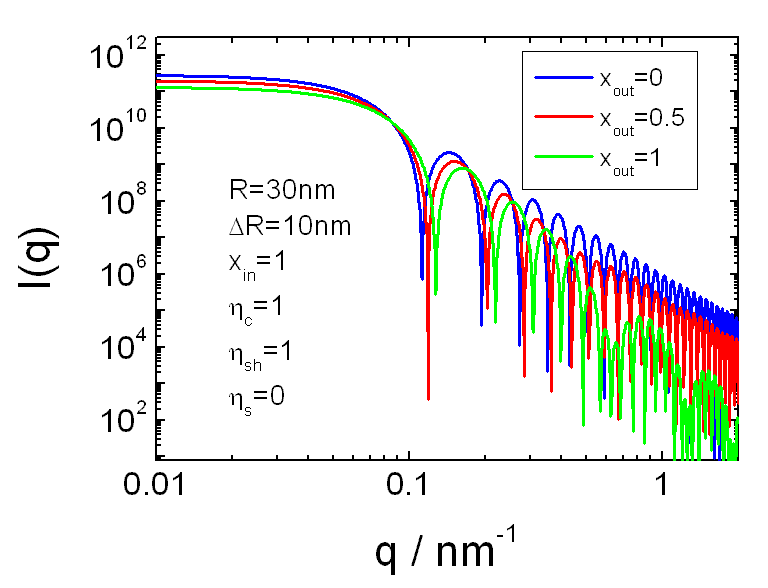
\includegraphics[width=0.768\textwidth,height=0.588\textwidth]{../images/form_factor/spheres/linshell1_Iq.png}
\end{center}
\caption{Scattering intensity of spheres with radius $R=30$nm, a shell thickness
of $\Delta R=10$nm, whereby the shell has a linear profile due to penetration
of solvent into the shell} \label{fig:I_LinShell1}
\end{figure}
%%%%%%%%%%%%%%%%%%%%%%%%%%%%%%%%%%%%%%%%%%%%%%%%%%%%%%%%%%%%%%%%%%%%%%%%%

\clearpage
\subsection{LinShell2}
\label{sect:LinShell2} ~\\

\begin{figure}[htb]
\begin{center}
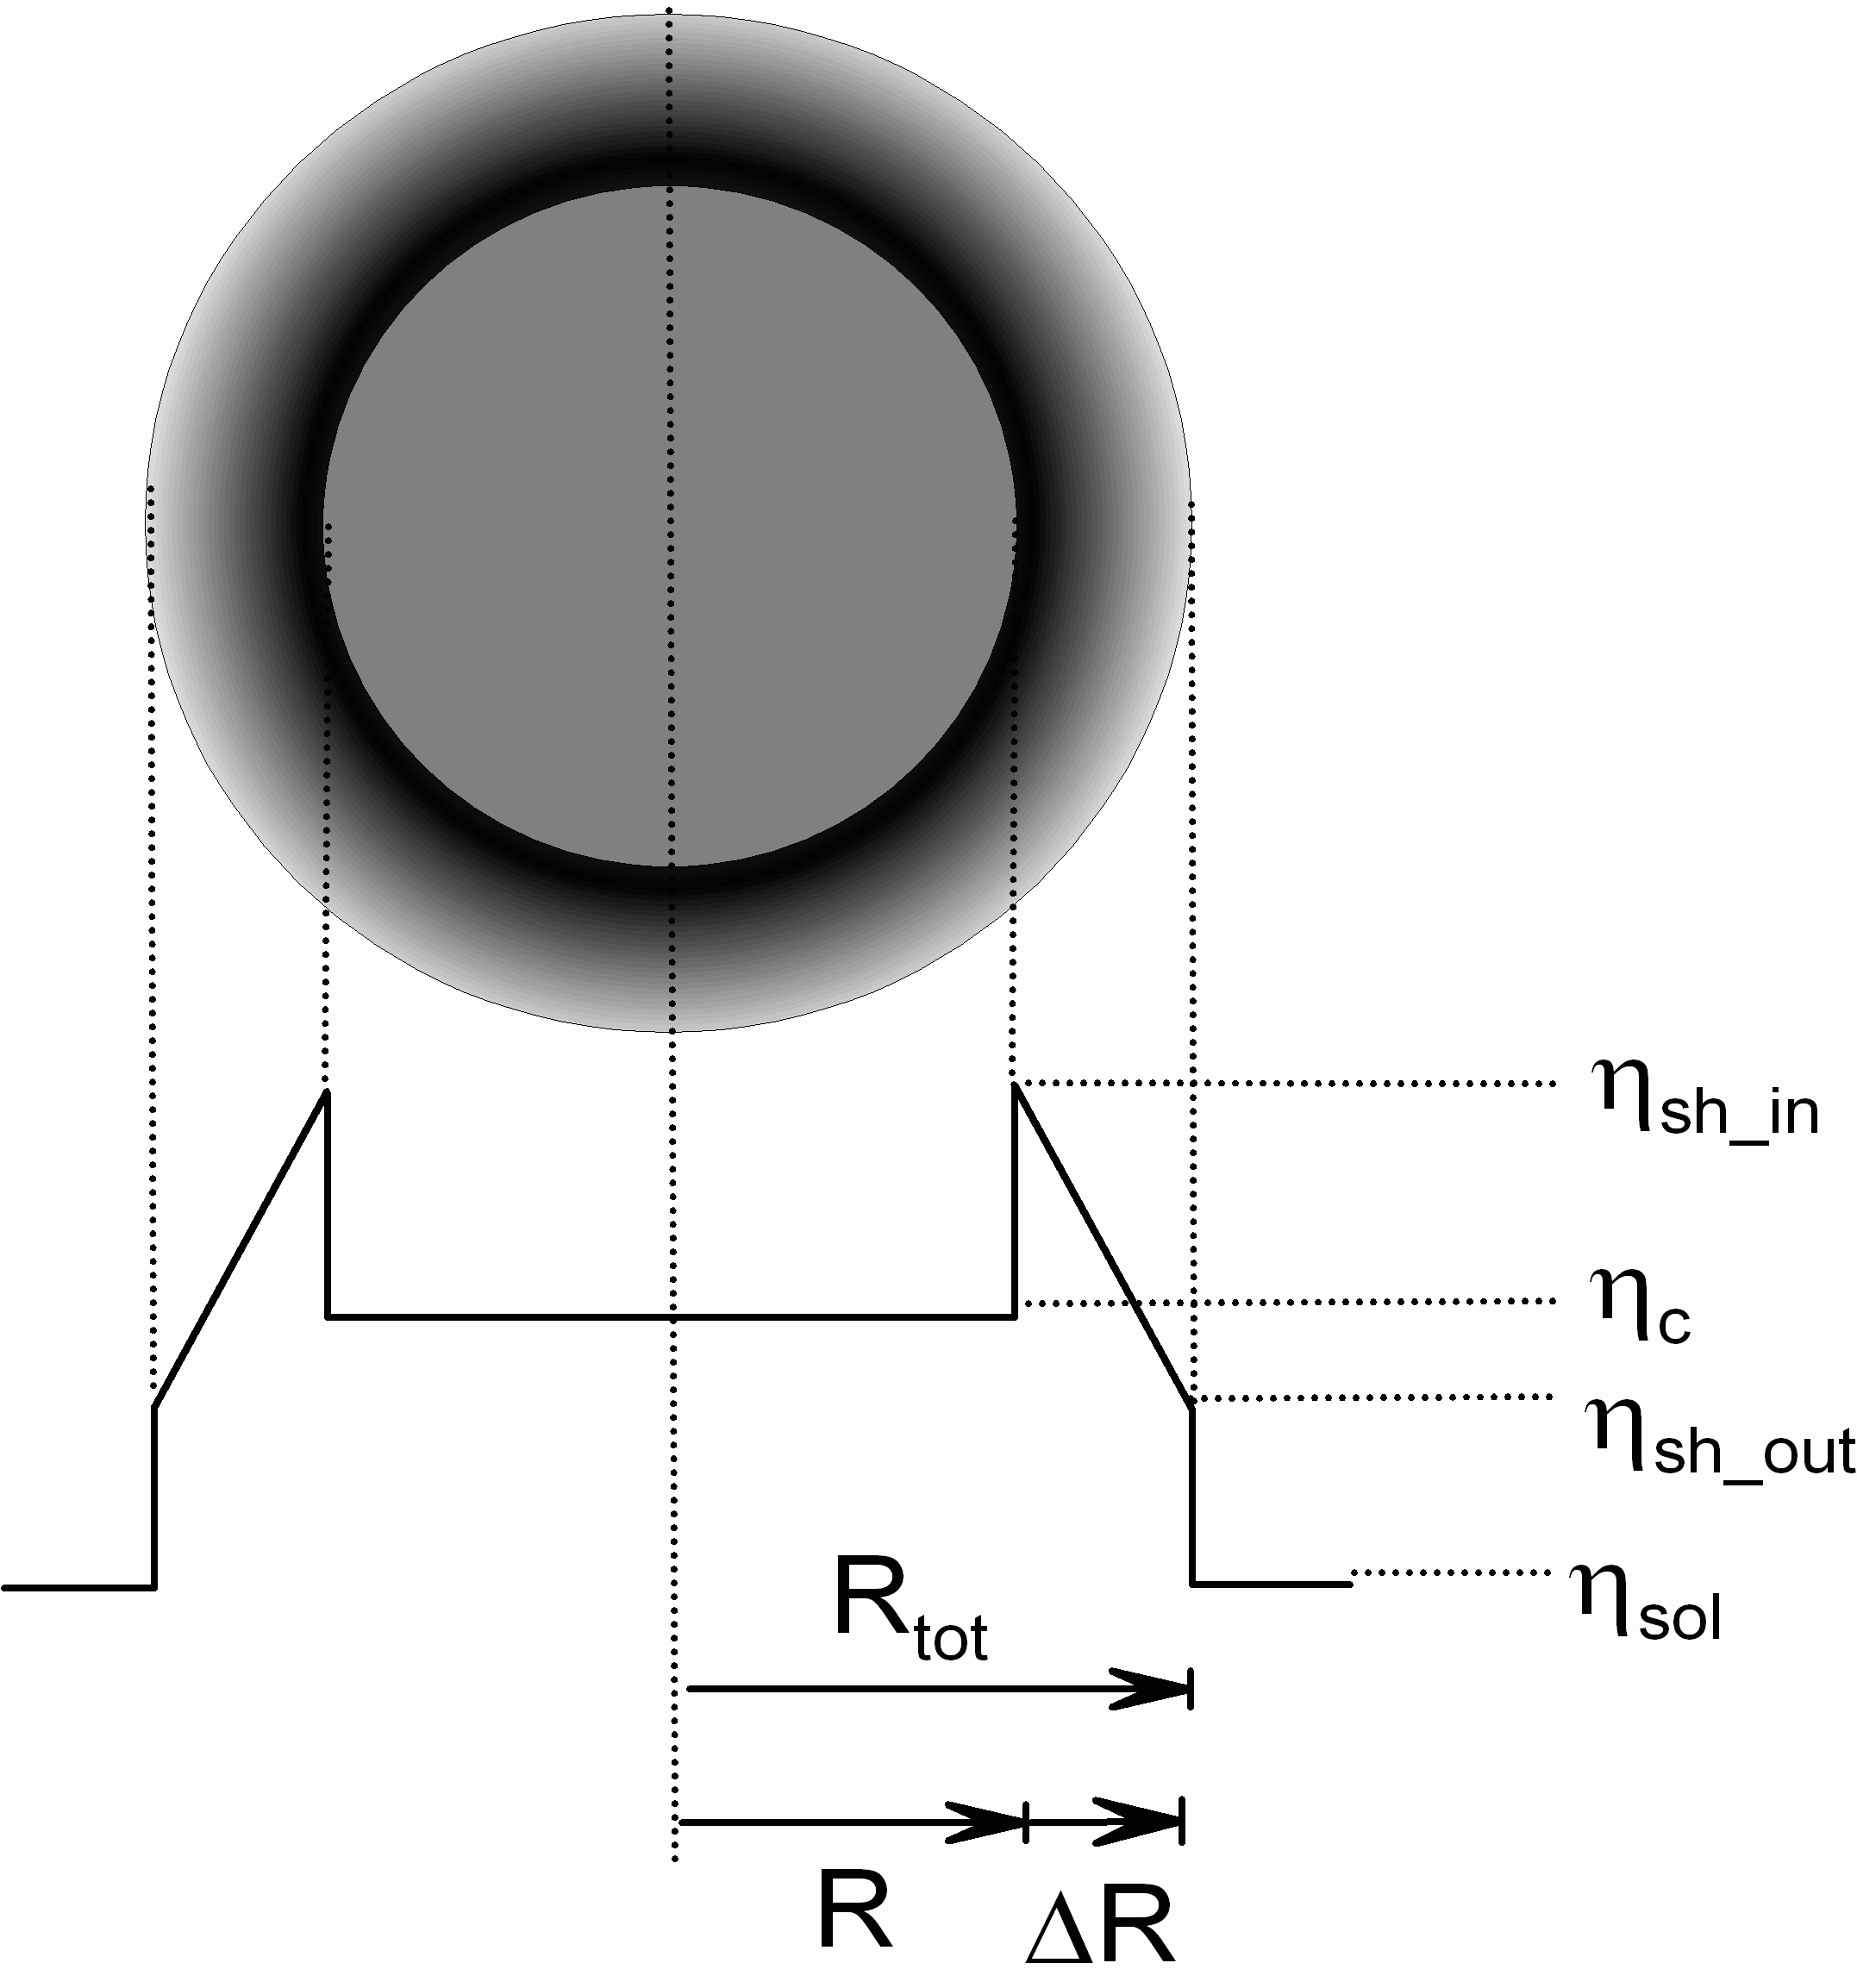
\includegraphics[width=0.5\textwidth,height=0.533\textwidth]{../images/form_factor/spheres/linshell2.png}
\end{center}
\caption{} \label{linshell}
\end{figure}

Form factor of a spherical shell with a total radius
$R_\text{tot}$ and a shell thickness of $\Delta R$. The definition
are the same than for {\tt LinShell} except that instead of the
core radius $R$ now the total radius $R_\text{tot}$ is used to
parameterize the form factor. The parameter definitions are the
following:

\begin{align}
R&=R_\text{tot}-\Delta R \\
\Delta\eta(r)      & =
\begin{cases}
\eta_\text{c}-\eta_\text{sol} & \text{~for~} r<R \\
m r + b  & \text{~for~} r \in [R,R_\text{tot}] \\
0 & \text{~for~} r>R_\text{tot}
\end{cases}
\\
m           & = (\eta_\text{sh\_out}-\eta_\text{sh\_in}) / \Delta R \\
b           & = -m R + \eta_\text{sh\_in} - \eta_\text{sol} \\
\eta_\text{sh\_in}  & = (1 - x_\text{in,sol})  \, \eta_\text{sh} + x_\text{in,sol} \,\eta_\text{sol} \\
                    & : \text{scattering length density at $R$} \nonumber \\
\eta_\text{sh\_out} & = (1 - x_\text{out,sol}) \, \eta_\text{sh} + x_\text{out,sol}\,\eta_\text{sol} \\
                    & : \text{scattering length density at $R_\text{tot}=R+\Delta R$} \nonumber \\
\eta_\text{sh}      & : \text{scattering length density of pure shell material} \nonumber \\
\eta_\text{c}       & : \text{scattering length density of core} \nonumber \\
x_\text{in,sol}     & : \text{amount of solvent at $R$} \nonumber \\
x_\text{out,sol}    & : \text{amount of solvent at $R_\text{tot}=R+\Delta R$} \nonumber
\end{align}

\begin{align}
F_\text{sph}(A,x) & = \frac{4}{3}\pi x^3 \,\, 3\frac{\sin(A)-A\cos(A)}{A^3} \\[5mm]
F_\text{shlin}(A,x) & = 4\pi x^4 \frac{2\cos(A)+2A\sin(A)-A^2\cos(A)}{A^4} \\[5mm]
I_\text{LinShell2}    & = \big[ \,\, (\eta_\text{c}-\eta_\text{sol}-b)F_\text{sph}(QR,R) \nonumber \\
             & \hspace{6mm} - mF_\text{shlin}(QR,R) \\
             & \hspace{6mm} + mF_\text{shlin}\left(QR_\text{tot},R_\text{tot}\right) \nonumber \\
             & \hspace{6mm} + bF_\text{sph}\left(QR_\text{tot},R_\text{tot}\right) \big]^2 \nonumber
\end{align}

\vspace{5mm}

\hspace{1pt}\\
\underline{Input Parameters for model \texttt{LinShell2}:}\\
\begin{description}
\item[\texttt{Rtot}] total overall radius $R_\text{tot}$
\item[\texttt{dR}] thickness of the shell $\Delta R$
\item[\texttt{eta\_c}] scattering length density $\eta_\text{c}$
\item[\texttt{eta\_sh}] scattering length density of non-swollen shell $\eta_\text{sh}$
\item[\texttt{x\_in}] amount of solvent $x_\text{in,sol}$ on core-shell interface at $R$ $(x_\text{in,sol} \in [0;1])$
\item[\texttt{x\_out}] amount of solvent $x_\text{out,sol}$ on shell-solvent interface at $R+\Delta R$ $(x_\text{out,sol} \in [0;1])$.
\item[\texttt{eta\_s}] scattering length density of solvent $\eta_\text{sol}$
\end{description}


\noindent\underline{Note:}
\begin{itemize}
\item $x_\text{in,sol}$ and $x_\text{out,sol}$ are only physical for values between 0 and 1.
\end{itemize}

%%%%%%%%%%%%%%%%%%%%%%%%%%%%%%%%%%%%%%%%%%%%%%%%%%%%%%%%%%%%%%%%%%%%%%%%%

\clearpage
\subsection{ExpShell}
\label{sect:ExpShell} ~\\

\begin{figure}[htb]
\begin{center}
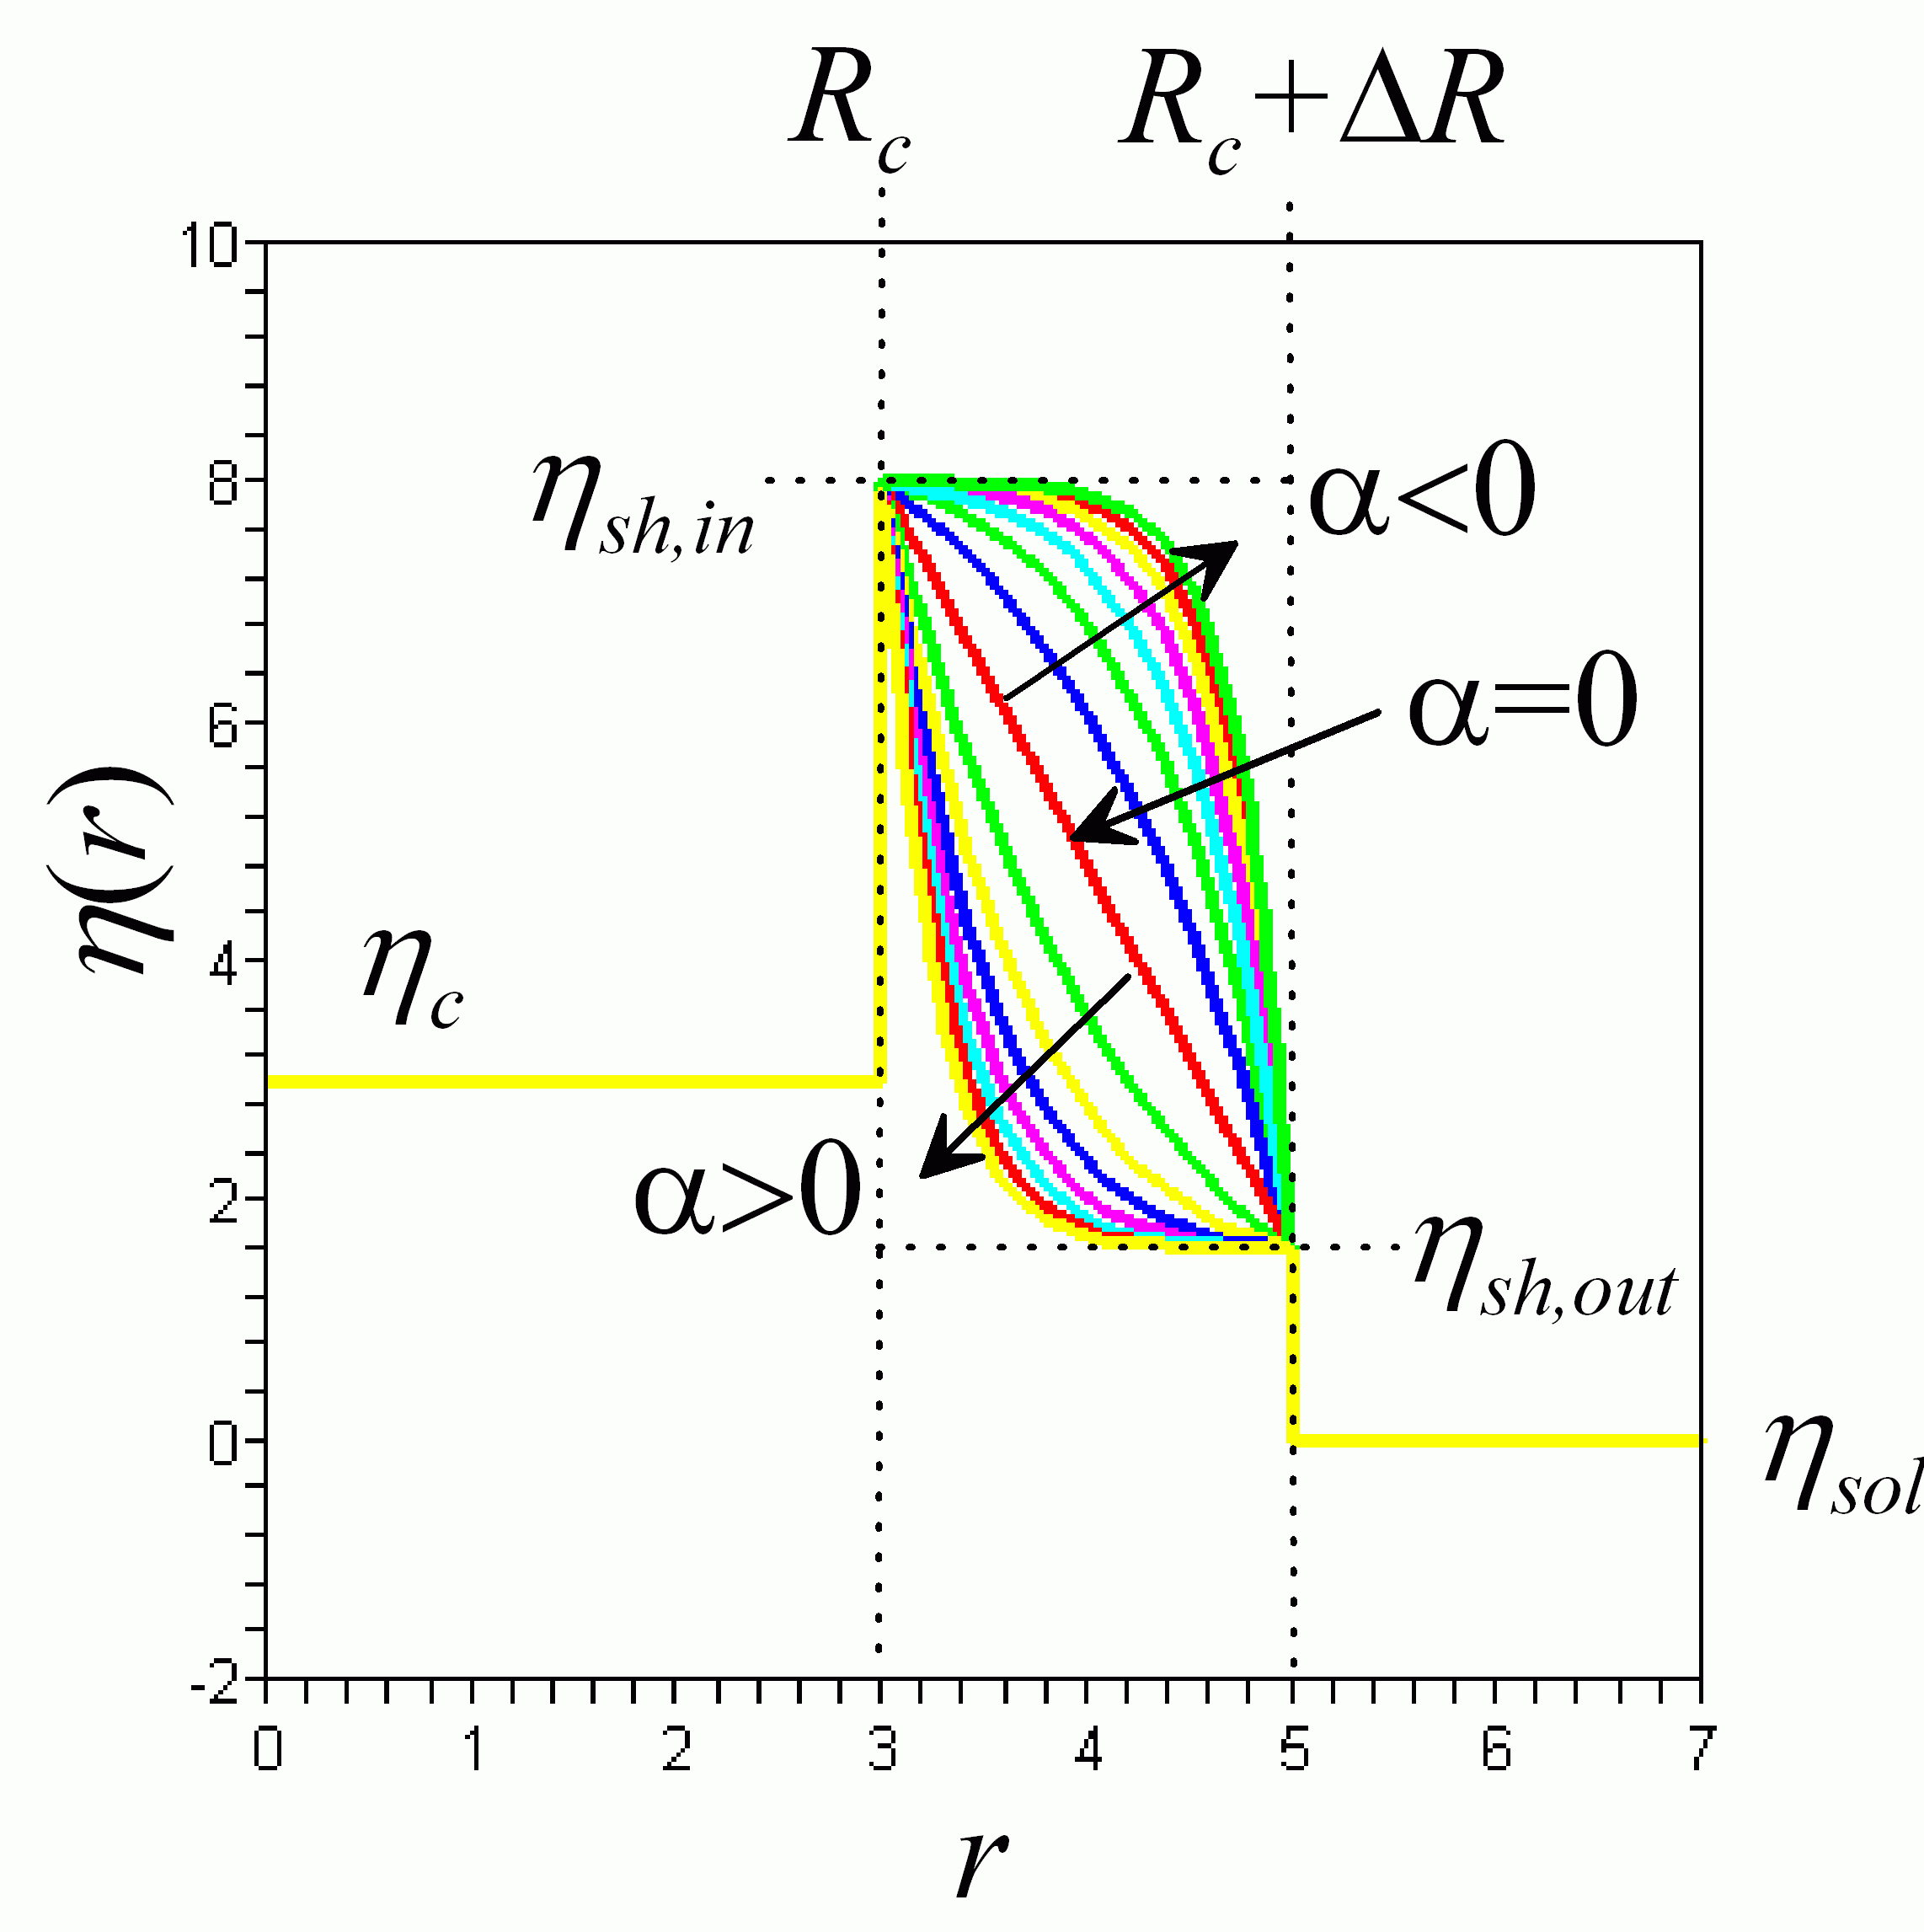
\includegraphics[width=0.55\textwidth,height=0.5\textwidth]{../images/form_factor/spheres/ExpShell.png}
\end{center}
\caption{} \label{linshell}
\end{figure}

\noindent
\begin{align}
\eta_\text{ExpShell}(r,R_c,\Delta R,\alpha,\phi_\text{in},\phi_\text{out}) &=
\begin{cases}
\eta_c              & r \leq R_c  \\
\eta_\text{exp}(\frac {r-R_c}{\Delta R})   & R_c < r< R_c+\Delta R \\
\eta_\text{sol}     & r> R_c+\Delta R
\end{cases}
\end{align}
\begin{align}
\eta_\text{exp} (x) &=
\begin{cases}
\eta_\text{sh,in}  +
\left[\eta_\text{sh,out}-\eta_\text{sh,in}\right] x \exp\left( \left[ 1-x \right] \alpha\right)
 & \alpha<0 \\[2mm]
\left[\eta_\text{sh,in}-\eta_\text{sh,out}\right] \left[1-x\right] \exp\left(-{x\alpha}\right) +
 \eta_\text{sh,out}& \alpha \geq 0
\end{cases} \\[2mm]
\eta_\text{sh,in} & = \left[ \phi_\text{in}\,\eta_\text{sol}+ \left( 1-\phi_\text{in} \right)
 \eta_\text{sh} \right] \\
\eta_\text{sh,out} & = \left[ \phi_\text{out}\,\eta_\text{sol}+ \left( 1-\phi_\text{out} \right) \eta_\text{sh} \right]
\end{align}

The scattering intensity for the radial symmetric scattering length density profile $\eta_\text{ExpShell}(r)$
can be calculated analytical. The integral needed to be solved for that is
\begin{equation}
I_\text{ExpShell}(Q) = \int_0^\infty 4\pi r^2 \frac{\sin Qr}{Qr}\, \eta_\text{ExpShell}(r)\, dr
\end{equation}

\begin{align}
R_c &=\text{core radius} \nonumber\\
\Delta R &=\text{shell thickness} \nonumber\\
\eta_\text{sh,in}  & = (1 - \phi_\text{in,sol})  \, \eta_\text{sh} + \phi_\text{in,sol} \,\eta_\text{sol} \\
                    & : \text{scattering length density at $R_c$} \nonumber \\
\eta_\text{sh,out}     & = (1 - \phi_\text{out,sol}) \, \eta_\text{sh} + \phi_\text{out,sol}\,\eta_\text{sol} \\
                        & : \text{scattering length density at $R_c+\Delta R$} \nonumber \\
\eta_\text{sh}      & : \text{scattering length density of pure shell material} \nonumber \\
\eta_\text{c}       & : \text{scattering length density of core} \nonumber \\
\phi_\text{in}     & : \text{amount of solvent  at $R_c$} \nonumber \\
\phi_\text{out}    & : \text{amount of solvent at $R_c+\Delta R$} \nonumber \\
\alpha             & : \text{parameter for exponential diffuse profile of the shell} \\
\nonumber
\end{align}


\vspace{5mm}

\hspace{1pt}\\
\underline{Input Parameters for model \texttt{ExpShell}:}\\
\begin{description}
\item[\texttt{R\_core}] radius of core  $R_c$
\item[\texttt{DR}] thickness of the shell $\Delta R$
\item[\texttt{eta\_core}] scattering length density $\eta_\text{c}$
\item[\texttt{eta\_shell}] scattering length density of non-swollen shell $\eta_\text{sh}$
\item[\texttt{x\_in\_sol}] amount of solvent $\phi_\text{in}$ on core-shell interface at $r=R$
\item[\texttt{x\_out\_sol}] amount of solvent $\phi_\text{out}$ on shell-solvent interface at $r=R+\Delta R$
\item[\texttt{alpha}]  a parameter ($\alpha$) which describes the penetration profile of the solvent into the shell.
A value of $\alpha=0$ means linear profile and is equivalent to {\tt LinShell} and {\tt LinShell2}. For $\alpha>0$
the solvent penetrates further into the shell and for $\alpha<0$ less.
\item[\texttt{eta\_solvent}] scattering length density of solvent $\eta_\text{sol}$
\end{description}

\noindent\underline{Note:}
\begin{itemize}
\item $\phi_\text{in}$ and $\phi_\text{out}$ are only physical for values between 0 and 1.
\end{itemize}

\begin{figure}[htb]
\begin{center}
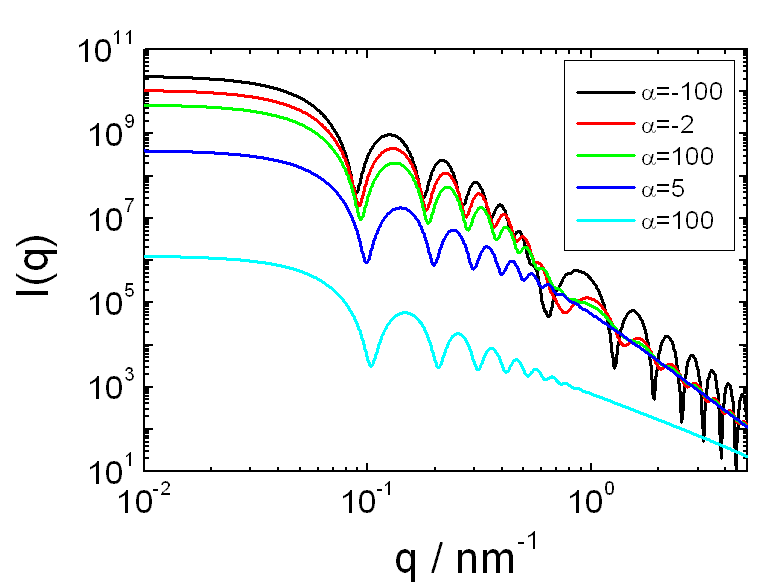
\includegraphics[width=0.768\textwidth,height=0.588\textwidth]{../images/form_factor/spheres/exp_shell.png}
\end{center}
\caption{Scattering intensity of a spherical shell with an exponential shell profile. The scattering intensity has been calculated
with a lognormal $[\mathrm{LogNorm}(N\!=\!1,\sigma\!=\!0.05,p\!=\!1,R\!=\!30)]$ size distribution for the core radius $R_c$.
The scattering length density of the core $\eta_\text{c}$ and the solvent $\eta_\text{sol}$ are set to 0, $\eta_\text{sh}=1$,
$\phi_\text{in}=0$, and $\phi_\text{out}=1$}
\label{fig:I_BiLayeredVesicle}
\end{figure}

\clearpage
\clearpage
\section{Ellipsoidal Objects}
\label{sect:EllipsoidalObjects}

\subsection{Ellipsoid with two equal semi-axis $R$ and semi-principal axes $\nu R$}
\label{sect:Ellipsoid_ii} ~\\


\begin{figure}[htb]
\begin{center}
%\includegraphics[width=0.706\textwidth,height=0.346\textwidth]{Elpsminr.png}
\includegraphics[width=0.5\textwidth,height=0.245\textwidth]{../images/form_factor/Ellipsoid/Elpsminr.png}
\end{center}
\caption{Ellipse, showing major and minor axes and parameters $a$ and $b$}
\label{minormajoraxes}
\end{figure}

An ellipsoid is a quadric surface in three dimensions obtained by
rotating an ellipse about one of its principal axes. Three
particular cases of an ellipsoid are:
\begin{itemize}
\item If the ellipse is rotated about its major axis, the surface is a prolate spheroid.
\item If the ellipse is rotated about its minor axis, the surface is an oblate spheroid.
\item If the generating ellipse is a circle, the surface is a sphere.
\end{itemize}

\begin{figure}[htb]
\begin{center}
\begin{minipage}[b]{0.5\linewidth}
\begin{center}
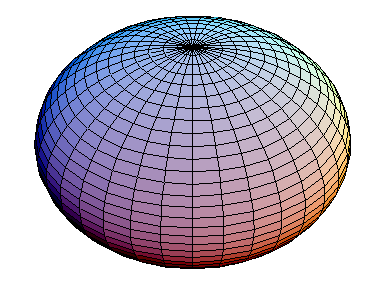
\includegraphics[width=7.5cm,height=5.7cm]{../images/form_factor/Ellipsoid/OblateSpheroid.png} \\
(a) oblate spheroid ($\nu <1$)
\end{center}
\end{minipage}%
\begin{minipage}[b]{0.5\linewidth}
\begin{center}
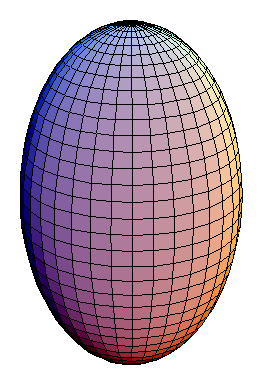
\includegraphics[width=5.1cm,height=7.5cm]{../images/form_factor/Ellipsoid/ProlateSpheroid.png}\\
(b) prolate spheroid ($\nu >1$)
\end{center}
\end{minipage}
\end{center}
\caption{A spheroid is an ellipsoid having two equal equatorial semi-axes. If the equatorial
semi-axis are larger than the principal axis the spheroid becomes oblate (a), if they are smaller
it becomes prolate (b) and if they are equal the spheroid becomes a perfect sphere}
\label{prolate oblate}
\end{figure}

\begin{align}
I_\text{ii}(Q,R,\nu) = \left( \frac{4}{3}\pi R^3 \Delta\eta
\right)^2
 \int_0^{\frac{\pi}{2}}\! K^2\left(Q,R\sqrt{\nu^2\cos^2\Theta+\sin^2\Theta}\right) \sin\Theta\, d\Theta
\end{align}
with $\DS \lim_{Q=0} I_\text{ii}(Q,R,\nu)= \left( \frac{4}{3}\pi
\nu R^3 \Delta\eta \right)^2 $

~\\
\underline{Input Parameters for model \texttt{Ellipsoid ii}:}
\begin{description}
\item[\texttt{R}] radius of the rotational axes
\item[\texttt{nu}]
ratio between radius of the semi-principle axes and equatorial axis.
Values of $\nu<1$ describe a oblate ellipsoid, a value of $\nu=1$ a
sphere, and $\nu>1$ a prolate ellipsoid.
\end{description}

\begin{figure}[htb]
\begin{center}
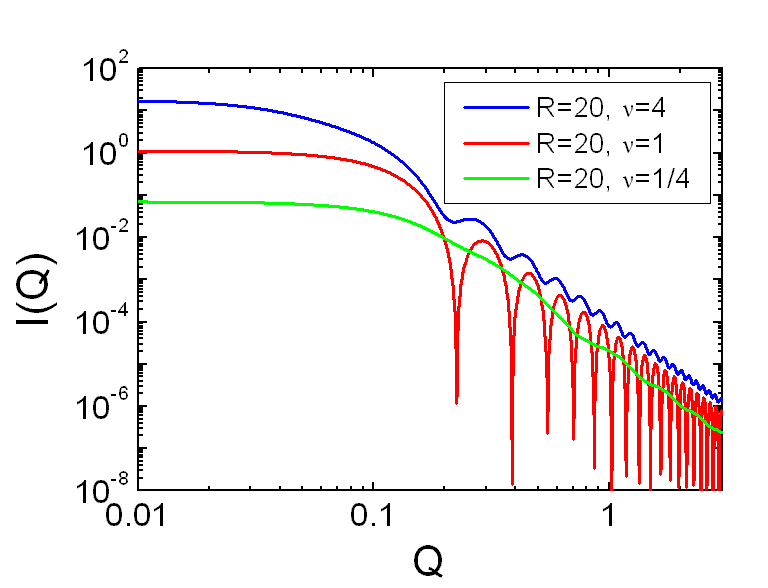
\includegraphics[width=0.768\textwidth,height=0.588\textwidth]{../images/form_factor/Ellipsoid/ellipsoid_ii.png}
\end{center}
\caption{form factor of an ellipsoid with axis $R$, $R$ and $\nu
R$.} \label{fig:I_ellipsoid_ii}
\end{figure}
%%%%%%%%%%%%%%%%%%%%%%%%%%%%%%%%%%%%%%%%%%%%%%%%%%%%%%%%
\clearpage
\subsection{Ellipsoid with two equal equatorial semi-axis $R$ and volume $V$}
\label{sect:Ellipsoid_i} ~\\

\begin{align}
I_\text{i}(Q,R,\nu) = \left( V \Delta\eta
\right)^2
 \int_0^{\frac{\pi}{2}}\! K^2\left(Q,R\sqrt{\nu^2\cos^2\Theta+\sin^2\Theta}\right)\sin\Theta\, d\Theta
\end{align}
with
$$
\nu=\frac{V}{R^3}\frac{3}{4\pi} \quad \mbox{so that}\quad V =\frac{4}{3}\pi\nu R^3
$$
and $\DS \lim_{Q=0} I_\text{i}(Q,R,\nu)= \left(V\Delta\eta\right)^2$

~\\
\underline{Input Parameters for model \texttt{Ellipsoid i}:}
\begin{description}
\item[\texttt{R}] radius of the rotational axes
\item[\texttt{V}] total volume of the ellipsoid.
\end{description}

\begin{figure}[htb]
\begin{center}
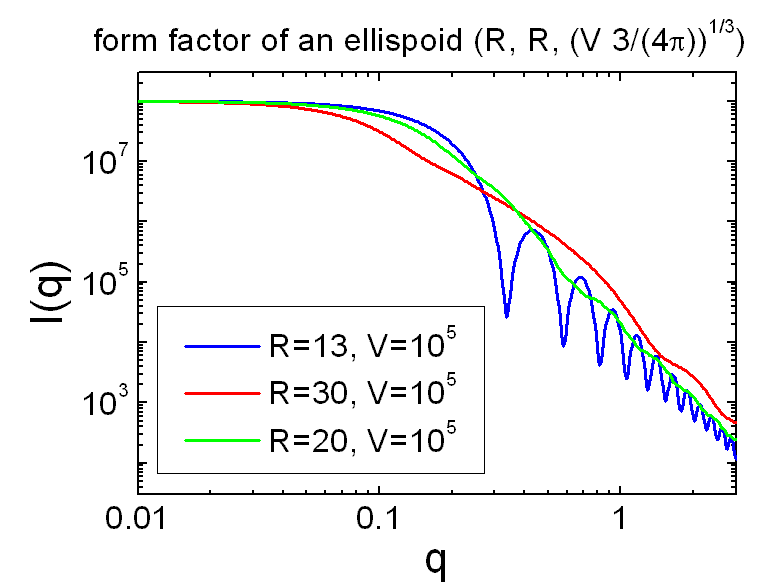
\includegraphics[width=0.768\textwidth,height=0.588\textwidth]{../images/form_factor/Ellipsoid/ellipsoid_i.png}
\end{center}
\caption{form factor of an ellipsoid with axis $R$, $R$ and
$\oldsqrt[3]{V\frac{3}{4\pi}}$.} \label{fig:I_ellipsoid_i}
\end{figure}
%%%%%%%%%%%%%%%%%%%%%%%%%%%%%%%%%%%%%%%%%%%%%%%%%%%%%%%%
\clearpage
\subsection{Ellipsoidal core shell structure}
\label{sect:EllipsoidalCoreShell} ~\\

\begin{figure}[htb]
\begin{center}
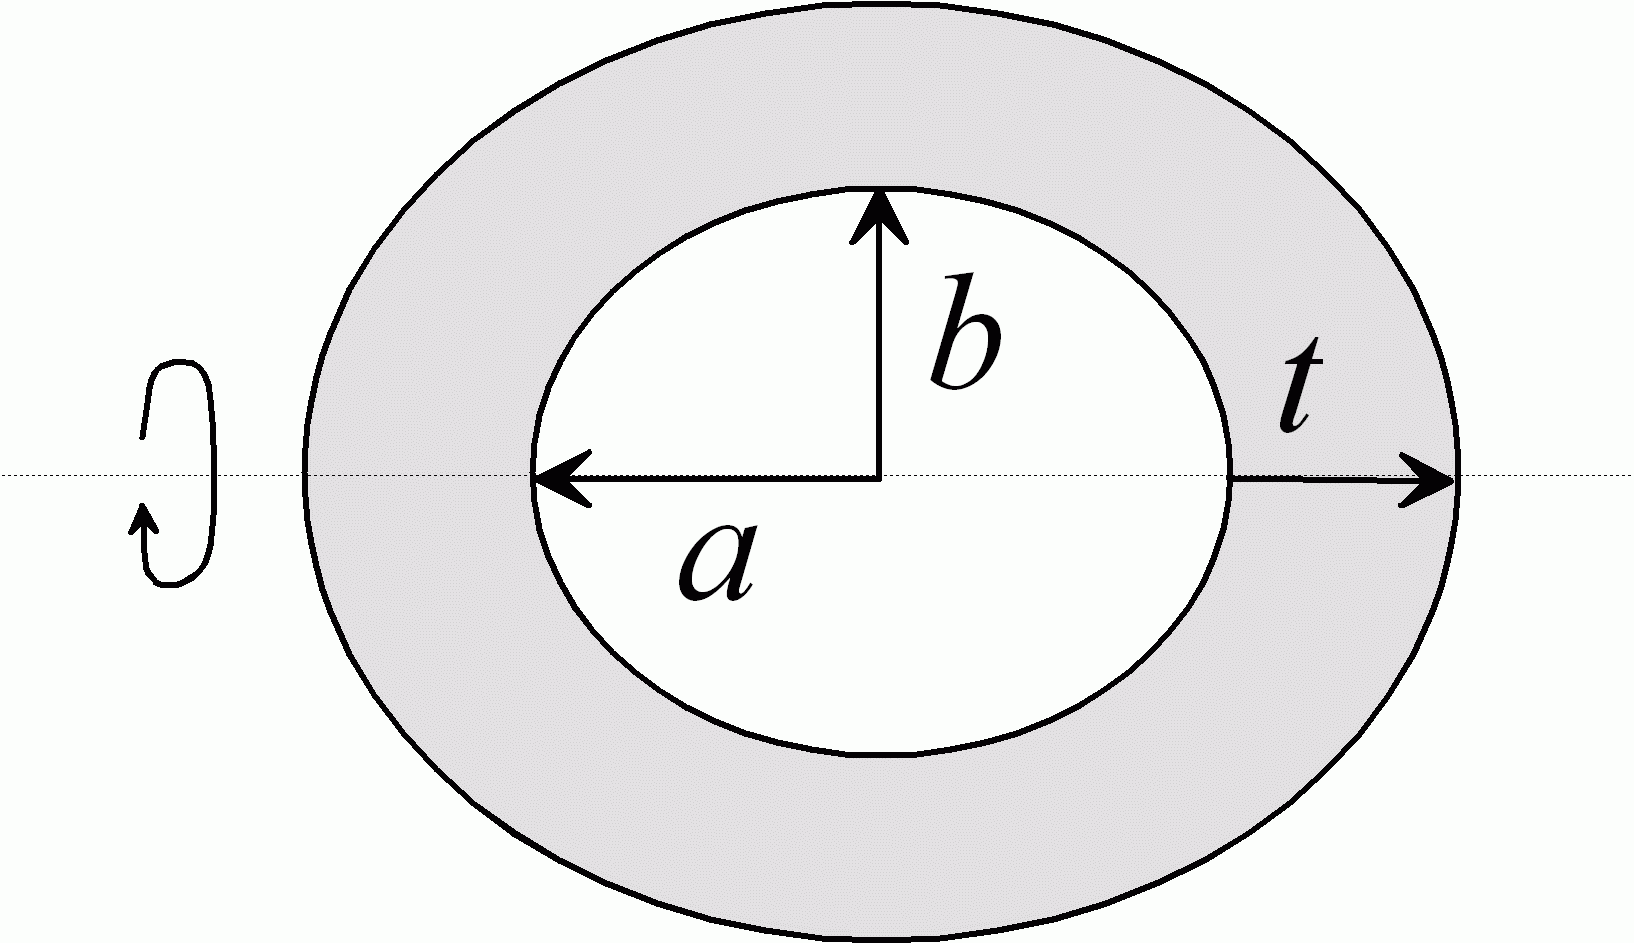
\includegraphics[width=0.5\textwidth,height=0.28855\textwidth]{ellipsoidalShell.png}
\end{center}
\caption{} \label{ellipsoidalShell}
\end{figure}
\begin{align}
I_\text{ECSh}(Q) = \left\langle F^2(Q,\mu) \right\rangle
& = \int_0^1 \left[F(Q,\mu)\right]^2 d\mu \\
\left\langle F(Q,\mu) \right\rangle^2 & = \left[\int_0^1 F(Q,\mu)
d\mu \right]^2
\end{align}
\begin{align}
F(Q,\mu) &= \left(\eta_\text{c}-\eta_\text{sh}\right) V_c\left[
\frac{3j_1(x_c)}{x_c}\right]
          +\left(\eta_\text{sh}-\eta_\text{sol}\right) V_t\left[ \frac{3j_1(x_t)}{x_t}\right]
          \nonumber \\
j_1(x) &= \frac{\sin(x)-x\cos(x)}{x^2} \nonumber \\
x_c &= Q \sqrt{a^2\mu^2+b^2(1-\mu^2)} \nonumber \\
x_c &= Q \sqrt{(a+t)^2\mu^2+(b+t)^2(1-\mu^2)} \nonumber \\
V_c &= \frac{4}{3}\pi ab^2 \nonumber \\
V_t &= \frac{4}{3}\pi (a+t)(b+t)^2 \nonumber
\end{align}
\begin{align}
\eta_\text{c} &: \text{scattering length density of core} \nonumber \\
\eta_\text{sh} &: \text{scattering length density of shell} \nonumber \\
\eta_\text{sol} &: \text{scattering length density of solvent} \nonumber \\
a &: \text{semi-principal axes of elliptical core} \nonumber \\
b &: \text{equatorial semi-axis of elliptical core} \nonumber \\
t &: \text{thickness of shell} \nonumber \\
V_c &: \text{volume of core} \nonumber \\
V_t &: \text{total volume of core along with shell} \nonumber
\end{align}

\vspace{0.5cm}

\underline{Input Parameters for model \texttt{EllipsoidalCoreShell}:}
\begin{description}
\item[\texttt{a}] semi-principal axes of elliptical core $a$
\item[\texttt{b}] equatorial semi-axis axes of elliptical core $b$
\item[\texttt{t}] thickness of shell $t$
\item[\texttt{eta\_c}] scattering length density of core $\eta_\text{c}$
\item[\texttt{eta\_sh}] scattering length density of shell $\eta_\text{sh}$
\item[\texttt{eta\_sol}] scattering length density of solvent $\eta_\text{sol}$
\end{description}

\begin{figure}[htb]
\begin{center}
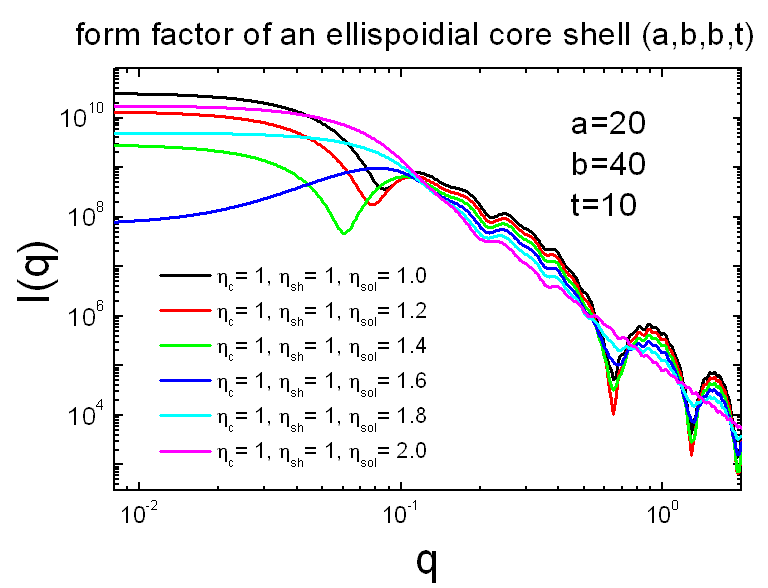
\includegraphics[width=0.768\textwidth,height=0.588\textwidth]{../images/form_factor/Ellipsoid/ellipsoidal_core_shell.png}
\end{center}
\caption{form factor of an ellipsoidal core shell $a$, $b$, $b$ and
$t$.} \label{fig:I_ellipsoidal_core_shell}
\end{figure}
%%%%%%%%%%%%%%%%%%%%%%%%%%%%%%%%%%%%%%%%%%%%%%%%%%%%%%%%
\clearpage
\subsection{triaxial ellipsoidal core shell structure}
\label{sect:triaxEllShell1} ~\\

\begin{figure}[htb]
\begin{center}
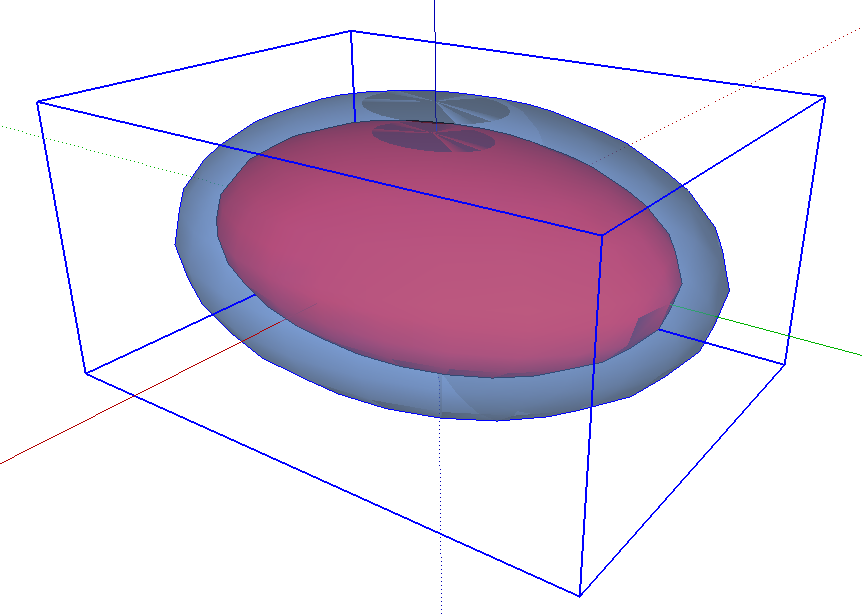
\includegraphics[width=0.45\textwidth,height=0.32177\textwidth]{../images/form_factor/Ellipsoid/triaxEll.png}
\hspace{0.08\textwidth}
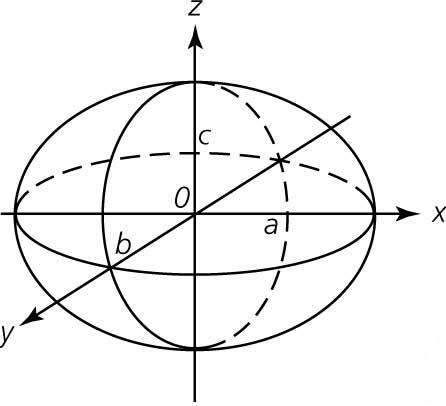
\includegraphics[width=0.45\textwidth,height=0.4096\textwidth]{../images/form_factor/Ellipsoid/A4ellipd.png}
\end{center}
\caption{triaxial ellipsoidal core shell structure} \label{triaEllShell}
\end{figure}

\begin{align}
I_\text{triaxEllSh}(Q) &= \int^1_0 \int ^1_0 dx\,dy\, K_\text{sh}^2(Q,R,R_t)\\
K(QR)         &= 3 \frac{\sin QR - QR\cos QR}{(QR)^3} \\
K_\text{sh}(Q,R,R_t) &= \left(\eta_\text{c}-\eta_\text{sh}\right)K(QR)+\left(\eta_\text{sh}-\eta_\text{sol}\right)K(QR_t) \\
R^2 &= \left[a^2\cos^2\left(\pi x/2\right) + b^2\sin^2\left(\pi x/2\right)\right](1-y^2)+c^2y^2 \nonumber \\
R_t^2 &= \left[(a+t)^2\cos^2\left(\pi x/2\right) + (b+t)^2\sin^2\left(\pi x/2\right)\right](1-y^2)+(c+t)^2y^2
\nonumber \\
V_c &= \frac{4}{3}\pi abc \nonumber \\
V_t &= \frac{4}{3}\pi (a+t)(b+t)(c+t) \nonumber
\end{align}
\begin{align}
\eta_\text{c} &: \text{scattering length density of core} \nonumber \\
\eta_\text{sh} &: \text{scattering length density of shell} \nonumber \\
\eta_\text{sol} &: \text{scattering length density of solvent} \nonumber \\
a &: \text{semi-axes of elliptical core} \nonumber \\
b &: \text{semi-axes of elliptical core} \nonumber \\
c &: \text{semi-axes of elliptical core} \nonumber \\
t &: \text{thickness of shell} \nonumber \\
V_c &: \text{volume of core} \nonumber \\
V_t &: \text{total volume of core along with shell} \nonumber
\end{align}

\vspace{3cm}
\underline{Input Parameters for model \texttt{triaxEllShell1}:}
\begin{description}
\item[\texttt{a}] semi-axes of elliptical core $a$
\item[\texttt{b}] semi-axes of elliptical core $b$
\item[\texttt{c}] semi-axes of elliptical core $c$
\item[\texttt{t}] thickness of shell $t$
\item[\texttt{eta\_c}] scattering length density of core $\eta_\text{c}$
\item[\texttt{eta\_sh}] scattering length density of shell $\eta_\text{sh}$
\item[\texttt{eta\_sol}] scattering length density of solvent $\eta_\text{sol}$
\end{description}

\begin{figure}[htb]
\begin{center}
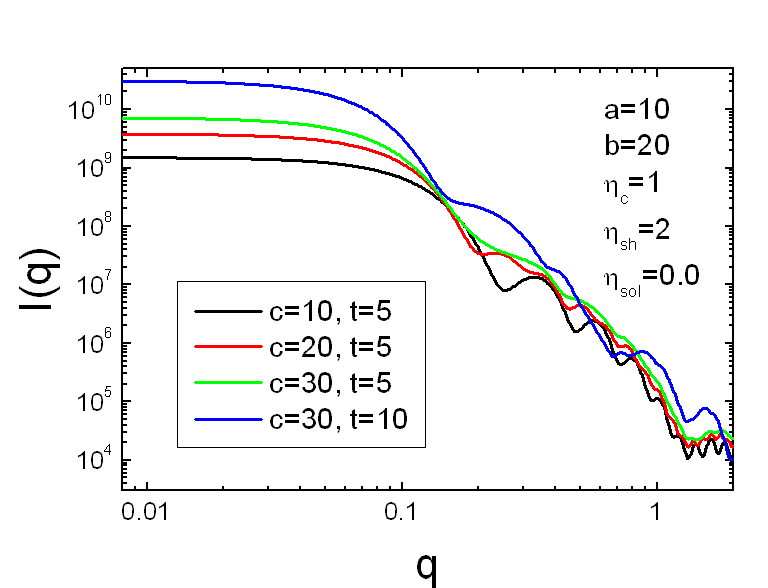
\includegraphics[width=0.768\textwidth,height=0.588\textwidth]{../images/form_factor/Ellipsoid/triax_ellipsoidal_core_shell.png}
\end{center}
\caption{Form factor of an triaxial ellipsoidal core shell with semi
axis $a$, $b$ and $c$ and a shell thickness $t$.}
\label{fig:I_ellipsoidal_core_shell}
\end{figure}

\clearpage
\section{Polymers and Micelles}
\label{sect:Polymers_Micelles}

\subsection{Gaussian chain}
\label{sect:GaussCoil}
~\\

\begin{figure}[htb]
\begin{center}
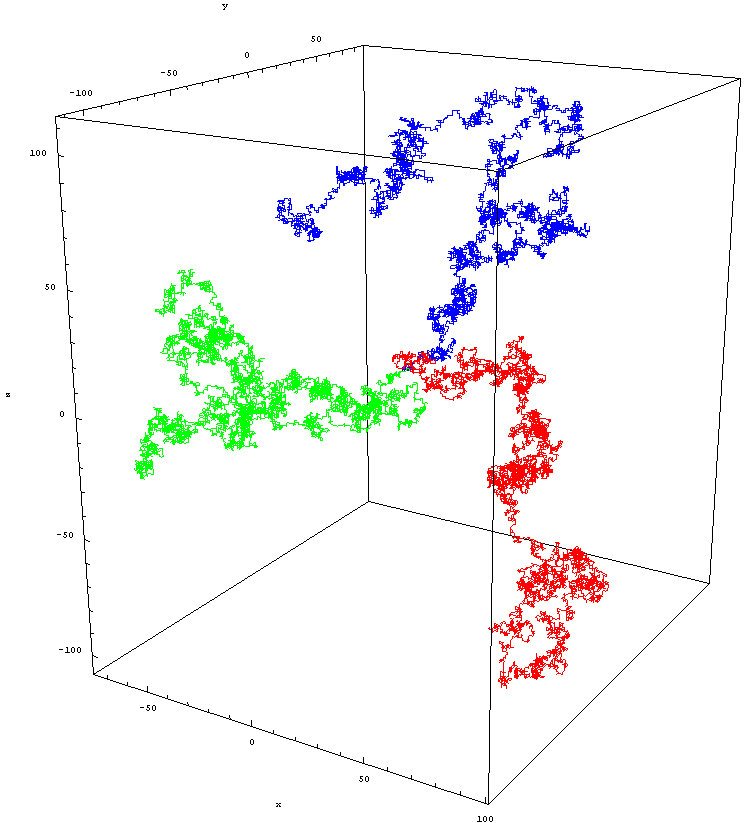
\includegraphics[width=0.744\textwidth,height=0.823\textwidth]{Walk3d_0.png}
\end{center}
\caption{The underlying model for a polymer chain is an
isotropic random walk on the euclidean lattice $\mathbb{Z}^3$.
This picture shows three different walks after 10 000 unit steps,
all three starting from the origin. \label{fig:RandomWalk3D}}
\end{figure}

Consider a flexible polymer coil where each monomer located at a
distance $\mathbf{R}_m$ its scattering field amplitude is given by
\begin{align}
F(\mathbf{q},t) &= \sum_{m=1}^N e^{-\imath
\mathbf{q}\cdot\mathbf{R}_m(t)} .
\end{align}
The scattering intensity averaged over all molecule configurations
reads
\begin{align}
\left\langle \abs{F(\mathbf{q})}^2\right\rangle
&= \sum_{m,n} \left\langle e^{-\imath\mathbf{q}\cdot(\mathbf{R}_m-\mathbf{R}_n)} \right\rangle
\end{align}
As the monomer segments $\mathbf{R}_m-\mathbf{R}_n$ are Gaussian distributed
the averages $\langle\cdots\rangle$ can be written as
\begin{subequations}
\begin{align}
\left\langle e^{-\imath\mathbf{q}\cdot(\mathbf{R}_m-\mathbf{R}_n)} \right\rangle
&= e^{\frac{q^2}{6}\left\langle \left( \mathbf{R}_m-\mathbf{R}_n\right)^2\right\rangle} \\
&= e^{-\frac{q^2b^2}{6}\abs{m-n}^{2\nu}}
\end{align}
\end{subequations}
Here $b$ is the statistical segment length and the contour length $L$ equals $L=Nb$.
The average of the segment inter-distances squares is kept in the general form
\begin{align}
\left\langle \left( \mathbf{R}_m-\mathbf{R}_n\right)^2\right\rangle
&= b^2 \abs{m-n}^{2\nu}.
\end{align}
$\nu$ is the excluded volume parameter from the Flory mean field
theory\footnote{P.J. Flory, "Statistical Mechanics of Chain Molecules", Interscience Publishers (1969)}\footnote{\href{http://www.ncnr.nist.gov/staff/hammouda/the_SANS_toolbox.pdf}{Boualem Hammouda, \texttt{the\_SANS\_toolbox.pdf}}}
of polymer solutions. The radius of gyration $R_G$ is given by
\begin{subequations}
\begin{align}
R_G^2 &= \frac{1}{2N^2}\sum_{m,n}^N \left\langle \left( \mathbf{R}_m-\mathbf{R}_n\right)^2\right\rangle \\
      &= \frac{1}{2N^2}\sum_{m,n}^N b^2 \abs{m-n}^{2\nu} \\
      &= \frac{b^2}{N} \sum_k^N \left(1-\frac{k}{N}\right) k^{2\nu} \\
      &= \frac{b^2}{\left(2\nu+1\right)\left(2\nu+2\right)} N^{2\nu}
\end{align}
\end{subequations}
Three cases are relevant:
\begin{enumerate}
\item Self-avoiding walk corresponds to swollen chains with $\nu = 3/5$, for which
$R_G^2=\frac{25}{176}b^2N^{6/5}$.
\item Pure random walk corresponds to chains in $\Theta$-conditions (where solvent-solvent,
monomer-monomer and solvent-monomer interactions are equivalent) with $\nu = 1/2$,
for which $R_G^2=\frac{1}{6}b^2N$.
\item Self attracting walk corresponds to collapsed chains with $\nu = 1/3$, for which
$R_G^2=\frac{9}{40}b^2N^{2/3}$.
\end{enumerate}
Using the general identity
\begin{align}
\sum_{i,j}^N y(\abs{i-j}) = N+2\sum_{k=1}^N(N-k) y(k)
\end{align}
the form factor reads
\begin{align}
P(q) &= \frac{1}{N^2}\abs{F(q)}^2 = \frac{1}{N^2}
\left\{N+2\sum_{k=1}^N(N-k)e^{-\frac{q^2b^2}{6}k^{2\nu}} \right\}
\end{align}
Going to the continuous limit $(N \gg 1)$, one obtains:
\begin{subequations}
\begin{align}
P(q) &= 2\int_0^1 \mathrm{d}x \; (1-x)e^{-\frac{q^2b^2}{6}N^{2\nu}x^{2\nu}} \\
&= \frac{U^{\frac{1}{2 \nu}} \Gamma\left(\frac{1}{2 \nu}\right)-
\Gamma\left(\frac{1}{\nu}\right)-U^{\frac{1}{2\nu}}
\Gamma\left(\frac{1}{2 \nu},U\right)+\Gamma\left(\frac{1}{\nu},U\right)}{\nu U^{1/\nu}} \\
&= \frac{1}{\nu U^{\frac{1}{2 \nu}}} \; \gamma\left(\frac{1}{2 \nu},U\right)-
   \frac{1}{\nu U^{\frac{1}{\nu}}}   \; \gamma\left(\frac{1}{  \nu},U\right)
\label{eq:generalizedGauss}
\end{align}
\end{subequations}
with the modified variable
\begin{align}
U&=\frac{q^2b^2N^{2\nu}}{6} = \left(2\nu+1\right)\left(2\nu+2\right)\frac{q^2R_G^2}{6}
\end{align}
and the upper incomplete Gamma Function $\Gamma(a,x) = \int_x^\infty \mathrm{d}t \; t^{a-1} \exp(-t)$ and lower incomplete Gamma Function $\gamma(a,x) = \int_0^x \mathrm{d}t \; t^{a-1} \exp(-t)$
for $a$ real and $x \geq 0$ and the Gamma function $\Gamma(a)=\Gamma(a,0)=\gamma(a,\infty)= \Gamma(a,x)+\gamma(a,x)=\int_0^\infty \mathrm{d}t\;  t^{a-1} \exp(-t)$.
Polymer chains follow Gaussian statistics in polymer solutions: they are swollen in good
solvents $\nu=3/5$, are thermally relaxed in "theta"-solvents $\nu=1/2$ and partially precipitate in poor solvents $\nu=1/3$.
The familiar Debye function is recovered when $\nu = 1/2$. The asymptotic limit at large $q$-values of the generalized
Gaussian chain is dominated by the $\frac{1}{\nu U^{\frac{1}{2\nu}}}\Gamma\left(\frac{1}{2\nu}\right)$
term which varies like $U^{-1/(2\nu)} \sim q^{-1/\nu}$. For $\nu =1$ we get the limit of an infinitesimal thin rod
and for $\nu=1/4$ a compact object with a Porod law of $q^{-4}$.

\SASfit has implemented the generalized form of a Gaussian (\texttt{generalized Gaussian coil}) coil and the standard
Debye formula \texttt{Gauss}. In both cases three version are implemented which only differ in their parametrization of
the forward scattering. In case of the the Debye-formula also the polydisperse \texttt{GaussPoly} is implemented.

\textcolor[rgb]{1.00,1.00,1.00}{Gauss}\\
\subsubsection{Gauss \cite{Debye1947}}
\label{sect:Gauss}
~\\
Flexible polymer chains which are not self-avoiding
and obey Gaussian statistics. Debye (1947) has calculated the form factor of such
chains:
\begin{align}
I_\text{Gauss}(q) &= I_0 2\frac{\exp(-u)+u-1}{u^2} \label{eq:DebyeGauss}\\
u &= q^2R_g^2
\end{align}

\vspace{5mm}
\underline{Input Parameters for model \texttt{Gauss}:}
\begin{description}
\item[\texttt{Rg}] radius of gyration $R_g$
\item[\texttt{I0}] forward scattering $I_0$ for $q=0$
\end{description}
\vspace{5mm}

\textcolor[rgb]{1.00,1.00,1.00}{Gauss}\\
\subsubsection{Gauss2 \cite{Debye1947}}
\label{sect:Gauss2}
~\\
This form factor differs only by the parametrization for the forward scattering
$I_0=(b_p-V\eta_\text{s})^2$ from the Debye formula in eq.\ \ref{eq:DebyeGauss}
\begin{align}
I_\text{Gauss2}(q) &= \beta^2 2\frac{\exp(-u)+u-1}{u^2} \\
u &= q^2R_g^2 \nonumber \\
\beta &= b_p-V\eta_\text{s}, \nonumber
\end{align}
where $b_p$ is the scattering length of a polymer molecule of molecular volume $V$ dissolved in a solvent
of scattering length density $\eta_\text{s}$ from which the excess scattering length of a polymer molecule
$\beta$ can be calculated. Combining this form factor with a \texttt{Delta} size distribution \ref{sec:Delta}
is needed to scale the scattering intensity. With proper values for the form factor the parameter $N$
of the \texttt{Delta}-distribution yields the particle number density.

\vspace{5mm}
\underline{Input Parameters for model \texttt{Gauss2}:}
\begin{description}
\item[\texttt{Rg}] radius of gyration $R_g$
\item[\texttt{b\_p}] scattering length of polymer $b_p$ in [cm]
\item[\texttt{V}] molecular volume of a single polymer molecule $V$ in [cm$^3$]
\item[\texttt{eta\_s}] scattering length density of solvent $\eta_\text{s}$ in [cm$^{-2}$]
\end{description}

\textcolor[rgb]{1.00,1.00,1.00}{Gauss}\\
\subsubsection{Gauss3 \cite{Debye1947}}
\label{sect:Gauss3}
~\\
This form factor differs only by the parametrization for the forward scattering
$I_0=(b_p-\frac{M_w}{N_a\rho_p}\eta_\text{s})^2$ from the Debye formula in eq.\ \ref{eq:DebyeGauss}
\begin{align}
I_\text{Gauss3}(q) &= \beta^2 2\frac{\exp(-u)+u-1}{u^2}
\end{align}
with
\begin{align}
u &= q^2R_g^2 \nonumber \\
\beta &= b_p-V\eta_\text{s} \nonumber\\
V &= \frac{M_w}{N_a\rho_p} \nonumber \\
N_a &= \mbox{Avogadro number} \nonumber
\end{align}

\underline{Input Parameters for model \texttt{Gauss3}:}
\begin{description}
\item[\texttt{Rg}] radius of gyration $R_g$
\item[\texttt{b\_p}] scattering length of polymer $b_p$ in [cm]
\item[\texttt{M\_w}] molecular weight of polymer $M_w$ in [g/mol]
\item[\texttt{rho\_p}] mass density of polymer $\rho_p$ in [g cm$^{-3}$]
\item[\texttt{eta\_s}] scattering length density of solvent $\eta_\text{s}$ in [cm$^{-2}$]
\end{description}

\begin{figure}[htb]
\begin{center}
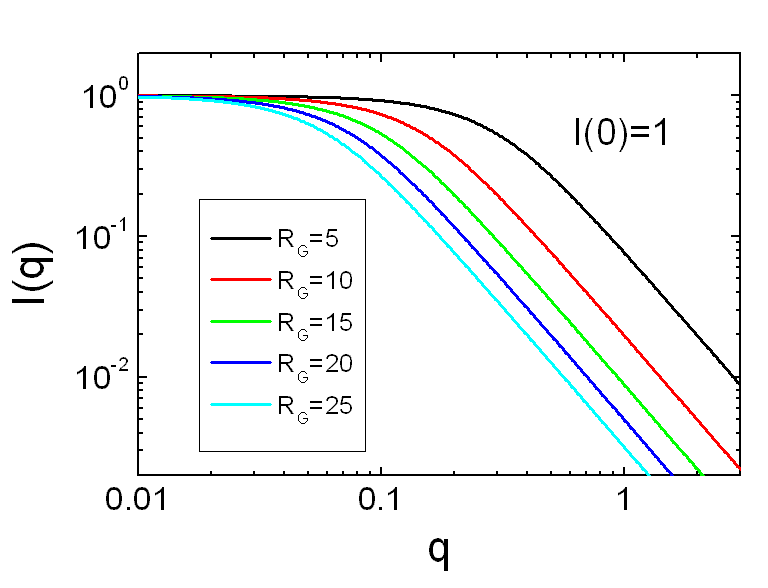
\includegraphics[width=0.768\textwidth,height=0.588\textwidth]{gaussian_coils.png}
\end{center}
\caption{Scattering function of Gaussian coils plotted for several radii of gyration.}
\label{fig:I_gaussian_coils}
\end{figure}

\textcolor[rgb]{1.00,1.00,1.00}{Gauss}\\
\subsubsection{Polydisperse flexible polymers with Gaussian statistics \cite{Pedersen2002}}  \label{sect:GaussPoly}
~\\
Polydispersity has been included in terms of a Schulz�Zimm mass distribution by
Zimm (1948) \cite{zimm:1093}  and Greschner (1973) \cite{Greschner1973}
~\\

\begin{align}
I_\text{GaussPoly}(q) &= I_0 2 \frac{\left( 1+U x\right)^{-1/U}+x-1}{(1+U)x^2} \\
x &= q^2R_g^2/(1+2U) \nonumber \\
U &= \frac{M_w}{M_n} -1 \nonumber
\end{align}

\vspace{5mm}
\underline{Input Parameters for model \texttt{GaussPoly}:}
\begin{description}
\item[\texttt{Rg}] radius of gyration $R_g$
\item[\texttt{M\_w}] weight averaged molecular weight $M_w$
\item[\texttt{M\_n}] number averaged molecular weight $M_n$
\item[\texttt{I0}] forward scattering $I_0$ for $q=0$
\end{description}

\begin{figure}[htb]
\begin{center}
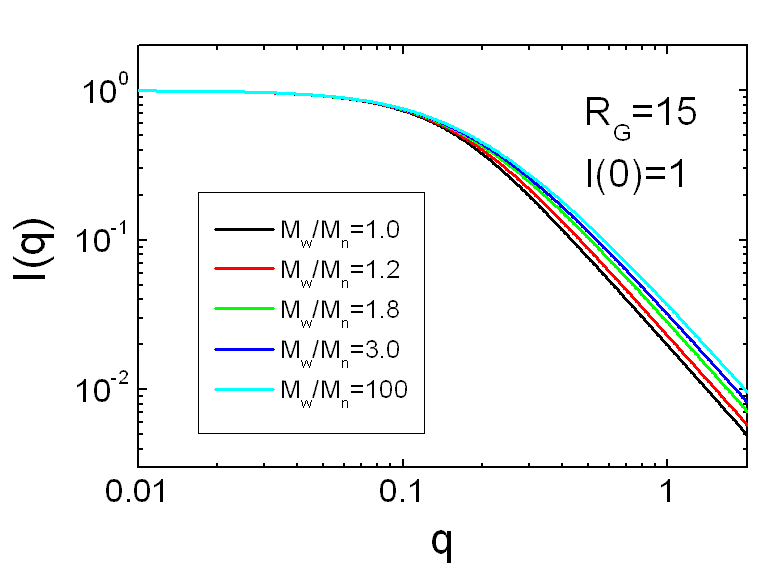
\includegraphics[width=0.768\textwidth,height=0.588\textwidth]{gauss_poly.png}
\end{center}
\caption{Scattering function of polydisperse Gaussian coil plotted for several ratios of $M_w/M_n$.}
\label{fig:I_gauss_poly}
\end{figure}

\textcolor[rgb]{1.00,1.00,1.00}{Gauss}\\
\subsubsection{generalalized Gaussian coil \cite{Hammouda,Hammouda2012,Hammouda1993,Hammouda2016}}
\label{sect:generalized_gaussian_coil}
~\\
The scattering function for the generalized Gaussian coil is according to eq.\ \ref{eq:generalizedGauss}
\begin{align}
I_\text{gGc}(q) &= I_0
\left(
\frac{1}{\nu U^{\frac{1}{2 \nu}}} \; \gamma\left(\frac{1}{2 \nu},U\right)-
\frac{1}{\nu U^{\frac{1}{  \nu}}} \; \gamma\left(\frac{1}{  \nu},U\right)
\right)
\label{eq:generalizedGauss1}
\end{align}
with the modified variable
\begin{align}
U&= \left(2\nu+1\right)\left(2\nu+2\right)\frac{q^2R_G^2}{6}
\end{align}
and the lower incomplete Gamma Function $\gamma(a,x) = \int_0^x \mathrm{d}t \; t^{a-1} \exp(-t)$.
$\nu$ is the excluded volume parameter from the Flory mean field theory and typical values for them are
\begin{description}
\item[$\nu=1/3$] partially precipitate in poor solvents
\item[$\nu=1/2$] thermally relaxed in "theta"-solvents
\item[$\nu=3/5$] swollen in good solvents
\end{description}

\vspace{5mm}
\underline{Input Parameters for model \texttt{generalized Gaussian coil}:}
\begin{description}
\item[\texttt{Rg}] radius of gyration $R_g$
\item[\texttt{nu}] excluded volume parameter $\nu\in [1/2;1]$
\item[\texttt{I0}] forward scattering $I_0$ for $q=0$
\end{description}
\vspace{5mm}


\subsubsection{generalized Gaussian coil 2 \cite{Hammouda,Hammouda2012}}
\label{sect:generalized_gaussian_coil2}
~\\
The scattering function for the generalized Gaussian coil is according to eq.\ \ref{eq:generalizedGauss}
and differs only by the parametrization for the forward scattering
$I_0=(b_p-V\eta_\text{s})^2$ from the formula in eq.\ \ref{eq:generalizedGauss1}
\begin{align}
I_\text{gGc2}(q) &= \left(b_p-V\eta_\text{s}\right)^2
\left(
\frac{1}{\nu U^{\frac{1}{2 \nu}}} \; \gamma\left(\frac{1}{2 \nu},U\right)-
\frac{1}{\nu U^{\frac{1}{  \nu}}} \; \gamma\left(\frac{1}{  \nu},U\right)
\right)
\label{eq:generalizedGauss2}
\end{align}
with the modified variable
\begin{align}
U&= \left(2\nu+1\right)\left(2\nu+2\right)\frac{q^2R_G^2}{6}
\end{align}

\vspace{5mm}
\underline{Input Parameters for model \texttt{generalized Gaussian coil 2}:}
\begin{description}
\item[\texttt{Rg}] radius of gyration $R_g$
\item[\texttt{b\_p}] scattering length of polymer $b_p$ in [cm]
\item[\texttt{V}] molecular volume of a single polymer molecule $V$ in [cm$^3$]
\item[\texttt{eta\_s}] scattering length density of solvent $\eta_\text{s}$ in [cm$^{-2}$]
\end{description}
\vspace{5mm}

\subsubsection{generalized Gaussian coil 3 \cite{Hammouda,Hammouda2012}}
\label{sect:generalized_gaussian_coil3}
~\\
The scattering function for the generalized Gaussian coil is according to eq.\ \ref{eq:generalizedGauss}
and differs only by the parametrization for the forward scattering
$I_0=(b_p-\frac{M_w}{N_a\rho_p}\eta_\text{s})^2$ from the formula in eq.\ \ref{eq:generalizedGauss1}
\begin{align}
I_\text{gGc3}(q) &= \left(b_p-\frac{M_w}{N_a\rho_p}\eta_\text{s}\right)^2
\left(
\frac{1}{\nu U^{\frac{1}{2 \nu}}} \; \gamma\left(\frac{1}{2 \nu},U\right)-
\frac{1}{\nu U^{\frac{1}{  \nu}}} \; \gamma\left(\frac{1}{  \nu},U\right)
\right)
\label{eq:generalizedGauss3}
\end{align}
with the modified variable
\begin{align}
U&= \left(2\nu+1\right)\left(2\nu+2\right)\frac{q^2R_G^2}{6}
\end{align}

\vspace{5mm}
\underline{Input Parameters for model \texttt{generalized Gaussian coil 3}:}
\begin{description}
\item[\texttt{Rg}] radius of gyration $R_g$
\item[\texttt{b\_p}] scattering length of polymer $b_p$ in [cm]
\item[\texttt{M\_w}] molecular weight of polymer $M_w$ in [g/mol]
\item[\texttt{rho\_p}] mass density of polymer $\rho_p$ in [g cm$^{-3}$]
\item[\texttt{eta\_s}] scattering length density of solvent $\eta_\text{s}$ in [cm$^{-2}$]
\end{description}
\vspace{5mm}

\begin{figure}[htb]
\begin{center}
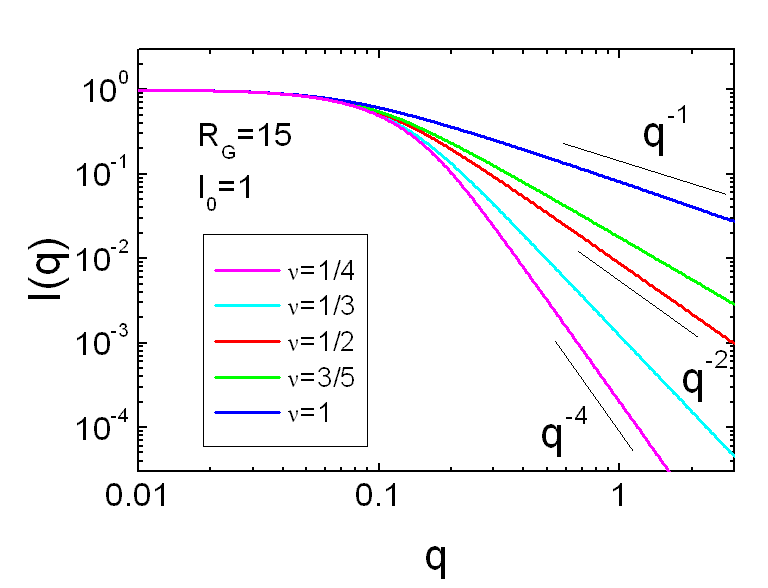
\includegraphics[width=0.768\textwidth,height=0.588\textwidth]{generalized_gaussian_coils.png}
\end{center}
\caption{Scattering function of the generalized Gaussian coil plotted for several excluded volume parameters.}
\label{fig:I_generalized_gaussian_coils}
\end{figure}
\clearpage

\subsection{Star polymer with Gaussian statistic according to
Benoit \cite{Benoit53}}
\label{sect:Benoit}
~\\

\begin{figure}[htb]
\begin{center}
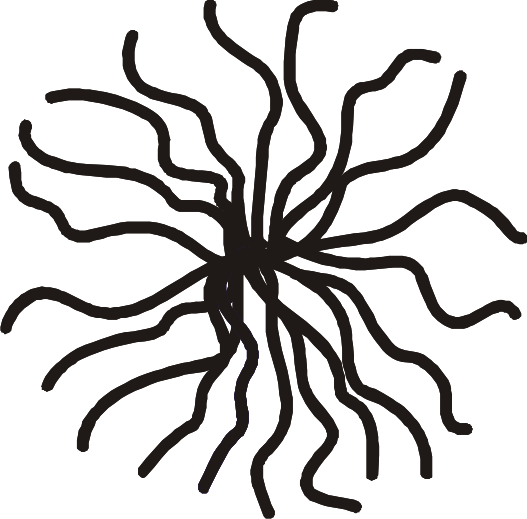
\includegraphics[width=0.2635\textwidth,height=0.2595\textwidth]{Benoit.png}
\end{center}
\caption{Sketch of a branched or star
polymers with $f$ number of arms} \label{fig:BenoitStar}
\end{figure}

Benoit \cite{Benoit53} derived an expression for the scattering from branched or star
polymers with a number of arms $f$, which can be expressed in the following way:
\begin{align}
I_\text{Star}(Q,R_G,f)= I_0 \frac{2}{f\nu^2}
    \left( \nu-\left[1-e^{-\nu}\right]+\frac{f-1}{2}\left[1-e^{-\nu}\right]^2\right)
\end{align}
with $\DS u=R_G^2Q^2$, $\DS \nu=\frac{uf}{3f-2}$ and $\DS
\lim_{Q=0}I_\text{Star}(Q,R_G,f)=I_0$. $f$
denotes the number of arms and $R_G$ the Guinier radius of a
single arm.

\vspace{5mm}

\noindent
\underline{Input Parameters for model \texttt{Benoit}:}
\begin{description}
\item[\texttt{RG}] radius of gyration of the star polymer $R_g$
\item[\texttt{f}] number of arms $f$
\item[\texttt{I0}] forward scattering $I_0$ for $q=0$
\end{description}


\begin{figure}[htb]
\begin{center}
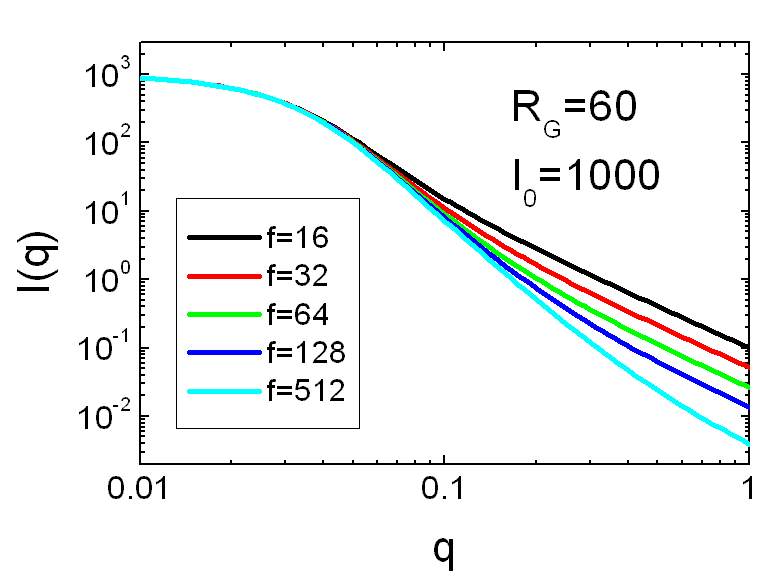
\includegraphics[width=0.768\textwidth,height=0.588\textwidth]{Benoit_Iq.png}
\end{center}
\caption{Scattering function of a star polymer according to Benoit. } \label{fig:Benoit_Iq}
\end{figure}

\clearpage

%\noindent REFERENCE:\\
%H.Benoit, J.Polym.Sci. 11(1953)507 \\


%%%%%%%%%%%%%%%%%%%%%%%%%%%%%%%%%%%%%%%%%%%%%%%%%%%%%%%%%%%%%%%%%%%%%

\subsection{Polydisperse star polymer with Gaussian statistics \cite{Burchard1974}}
\label{sect:PolydisperseStar}
~\\
\begin{figure}[htb]
\begin{center}
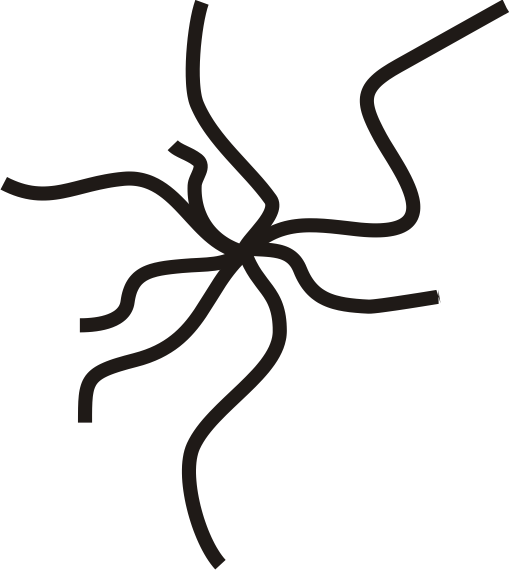
\includegraphics[width=0.2545\textwidth,height=0.2535\textwidth]{polyBenoit.png}
\end{center}
\caption{Polydisperse star polymer with Gaussian statistics} \label{fig:polyBenoitStar}
\end{figure}

For a Schulz�Flory (most probable) distribution (Schulz�Zimm distribution
with $z = 1$) for the mass distribution of the arms, Burchard \cite{Burchard1974} has given the form factor:
\begin{align}
I_\text{PolydisperseStar}(Q) &= I_0
\frac{1+\frac{u^2}{3 f}}{\left(1+\frac{u^2(f +1)}{6 f }\right)^2}
\end{align}
where $f$ is the number of arms and $u^2 = \langle R_g^2 \rangle_z \,Q^2$, where
$\langle R_g^2 \rangle_z$ is the $z$-average radius of gyration squared of an arm.

\vspace{5mm}

\noindent
\underline{Input Parameters for model \texttt{PolydisperseStar}:}
\begin{description}
\item[\texttt{R\_G}] radius of gyration $R_G$
\item[\texttt{f}] number of arms $f$
\item[\texttt{I0}] forward scattering $I_0$
\end{description}


\begin{figure}[htb]
\begin{center}
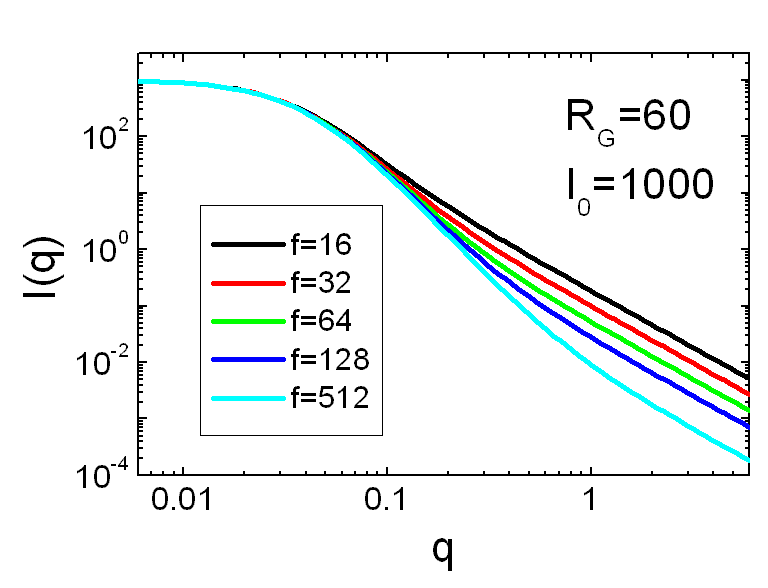
\includegraphics[width=0.768\textwidth,height=0.588\textwidth]{polyBenoit_Iq.png}
\end{center}
\caption{Scattering function of a polydisperse star polymer with Gaussian statistics.} \label{fig:polyBenoit_Iq}
\end{figure}

\clearpage

%%%%%%%%%%%%%%%%%%%%%%%%%%%%%%%%%%%%%%%%%%%%%%%%%%%%%%%%%%%%%%%%%%%%%%%%%%%%%%%%%%%%%%%%

\subsection{Star polymer according to Dozier \cite{dozier91}}
\label{sect:DozierStar}
~\\
\subsubsection{Dozier}
\label{sect:DozierStar1}
~\\
\begin{figure}[htb]
\begin{center}
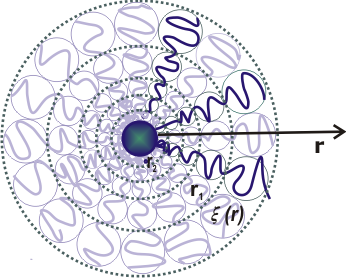
\includegraphics[width=0.346\textwidth,height=0.278\textwidth]{Dozier.png}
\end{center}
\caption{Star polymer according to Dozier} \label{fig:DozierStar}
\end{figure}
Branched polymers having all branches emanating from
the center of the macromolecule are commonly called star
polymers. For a star polymer Dozier \cite{dozier91} has developed
a scattering function which reads:
\begin{align}
I_\text{DozierStar}(Q,I_0,R_G,\alpha,\nu,\xi)
& = I_0 \exp\left(-\frac{Q^2R_G^2}{3}\right) \\
+& \frac{4\pi\alpha}{Q\xi} \Gamma(\mu)
\frac{\sin(\mu\arctan(Q\xi))}{(1+Q^2\xi^2)^{\mu/2}} \nonumber
\end{align}
with $\mu=1/\nu-1$
\begin{align}
R_G      & : \text{radius of gyration} \nonumber \\
I_0      & : \text{scale parameter} \nonumber \\
\alpha   & : \text{scale parameter for fractal term} \nonumber \\
\xi      & : \text{exponential damping length in mass fractal} \nonumber \\
\nu      & : \text{Flory exponent, 3/5 in good solvent, 1/2 in
theta solvent (i.e. $\mu=2/3$ to 1)} \nonumber
\end{align}

\vspace{5mm}

\noindent
\underline{Input Parameters for model \texttt{Dozier}:}
\begin{description}
\item[\texttt{R\_G}] radius of gyration $R_G$
\item[\texttt{I\_0}] scale parameter $I_0$
\item[\texttt{alpha}] scale parameter for fractal term $\alpha$
\item[\texttt{xi}] exponential damping length in mass fractal $\xi$
\item[\texttt{nu}] excluded volume parameter or Flory exponent $\nu$
\end{description}
\vspace{5mm}

\begin{figure}[htb]
\begin{center}
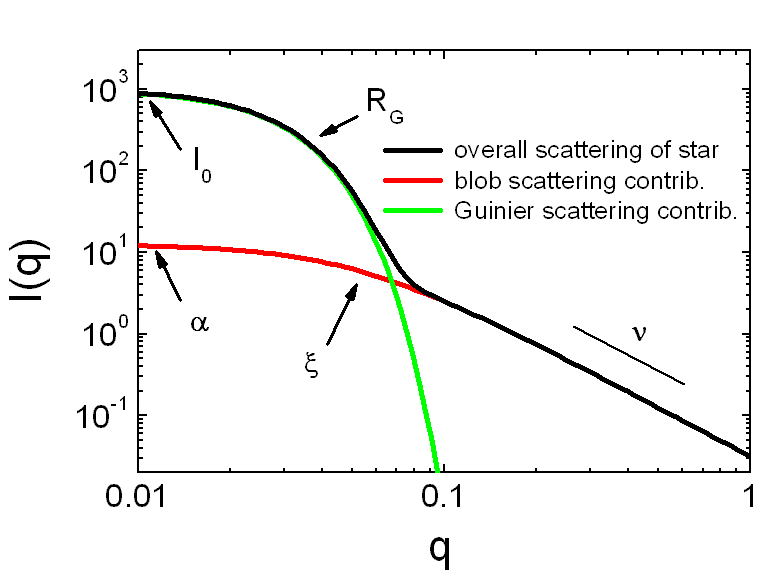
\includegraphics[width=0.768\textwidth,height=0.588\textwidth]{Dozier_Iq.png}
\end{center}
\caption{Scattering function of a star polymer according to Dozier: $I0=10^3$, $R_g=60$, $\alpha=1$
$\xi=20$, $\nu=1/2$ } \label{fig:IQDozierStar1}
\end{figure}

\clearpage

\subsubsection{Dozier2}
\label{sect:DozierStar2}
~\\
This is a re-parametrization of the \texttt{Dozier} form factor
to scale the scattering of the overall star to the local scattering of the individual arms.
\begin{align}
I_\text{DozierStar2}(Q,I_0,R_G,N_\text{agg},\nu,\xi)=
\frac{I_0}{N_\text{agg}}
\Biggl(
 &  (N_\text{agg}-1)
    \exp\left(-\frac{Q^2R_G^2}{3}\right) \\
 +&  \frac{\Gamma(\mu)}{Q\xi}
    \frac{\sin(\mu\arctan(Q\xi))}{(1+Q^2\xi^2)^{\mu/2}} \nonumber
\Biggr)
\end{align}
with $\mu=1/\nu-1$
\begin{align}
R_G      & : \text{radius of gyration of the star} \nonumber \\
I_0      & : \text{scale parameter} \nonumber \\
N_\text{agg} & : \text{number of arms in the star} \nonumber \\
\xi      & : \text{exponential damping length in mass fractal} \nonumber \\
\nu      & : \text{Flory exponent, 3/5 in good solvent, 1/2 in
theta solvent (i.e. $\mu=2/3$ to 1)} \nonumber
\end{align}

\vspace{5mm}

\noindent
\underline{Input Parameters for model \texttt{Dozier2}:}
\begin{description}
\item[\texttt{R\_G}] radius of gyration of the star $R_G$
\item[\texttt{I\_0}] scale parameter $I_0$
\item[\texttt{Nagg}]  number of arms $N_\text{agg}$ in the star from which the scale parameter for fractal term is calculated
\item[\texttt{xi}] exponential damping length in mass fractal $\xi$
\item[\texttt{nu}] Flory exponent, $\nu=3/5$ in good solvent, $\nu=1/2$ in
theta solvent (i.e. $\mu=2/3$ to 1)
\end{description}
\vspace{5mm}

\begin{figure}[htb]
\begin{center}
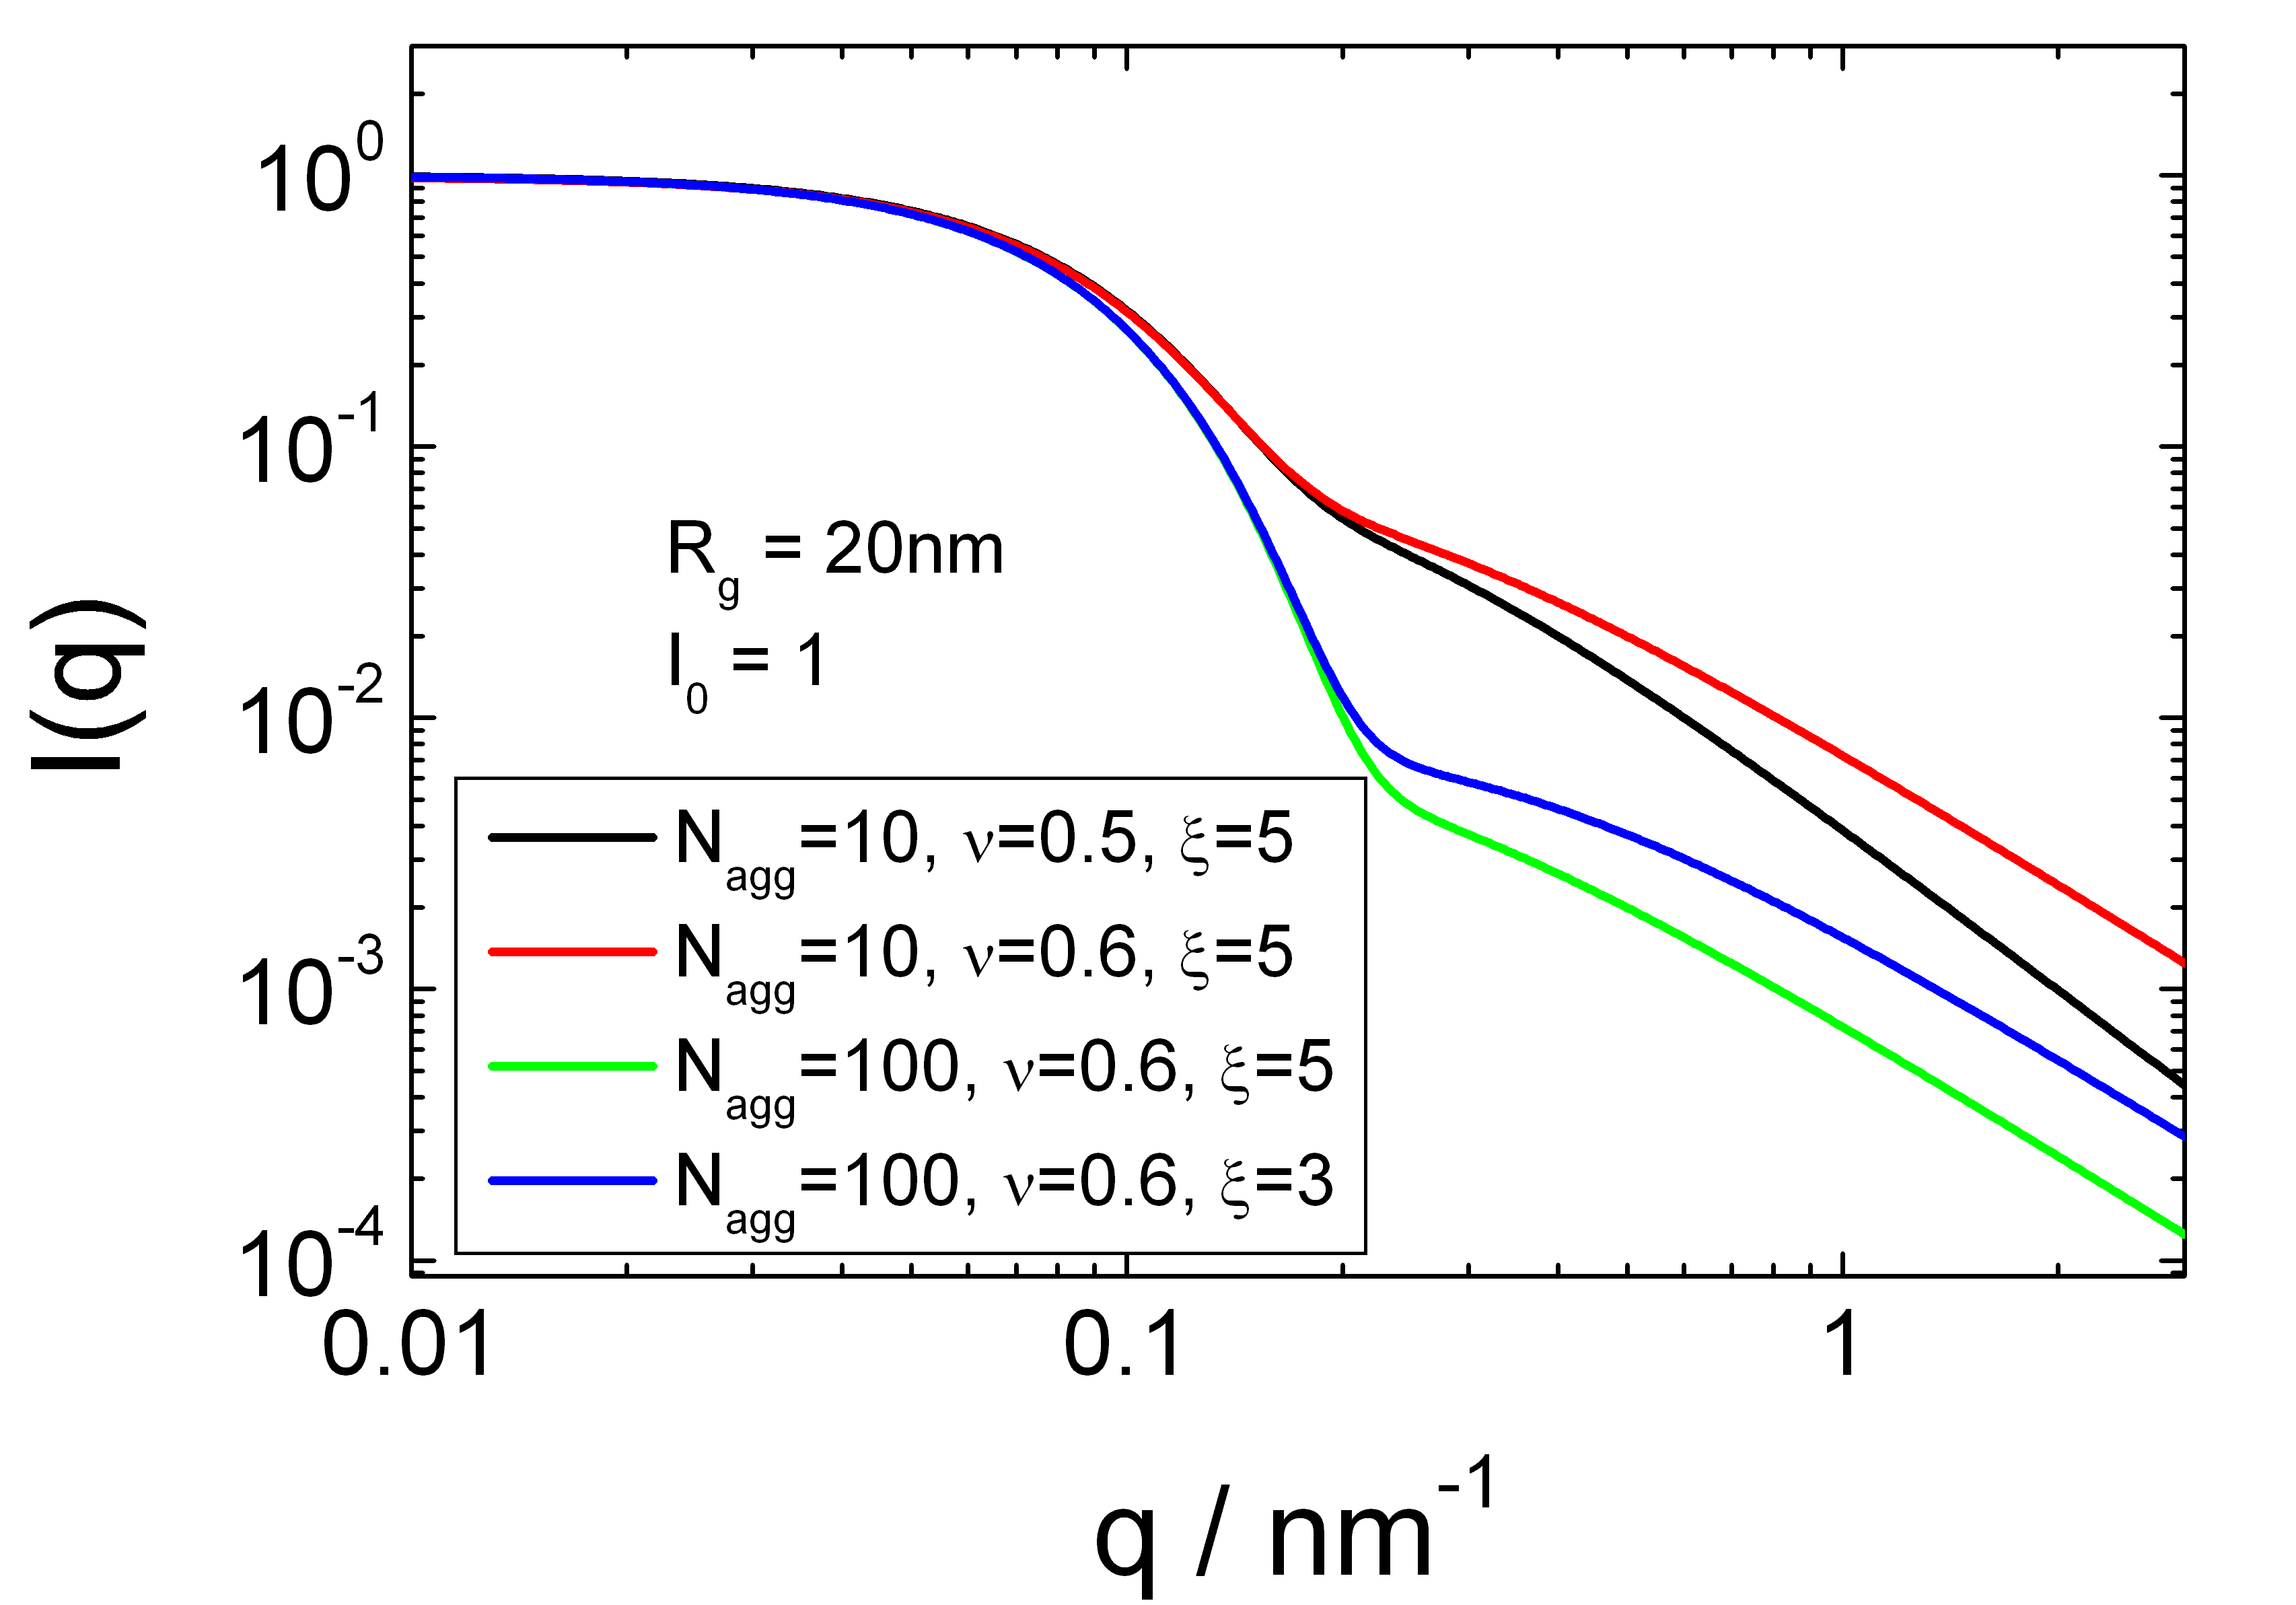
\includegraphics[width=0.768\textwidth,height=0.588\textwidth]{Dozier2_Iq.png}
\end{center}
\caption{Scattering function of a star polymer according to Dozier but modified
to scale the scattering of the overall star to the local scattering of the individual arms
by the number of arms} \label{fig:IQDozierStar2}
\end{figure}
\clearpage

%\noindent REFERENCE:\\
%W.D.Dozier, J.S.Huang \& L.J.Fetters, Macromolecules
%24(1991)2810-2814

%%%%%%%%%%%%%%%%%%%%%%%%%%%%%%%%%%%%%%%%%%%%%%%%%%%%%%%%%%%%%%%%%%%%%%%%


\subsection{Flexible Ring Polymer \cite{Burchard1996}}
\label{sect:FlexibleRingPolymer}
~\\

\begin{figure}[htb]
\begin{center}
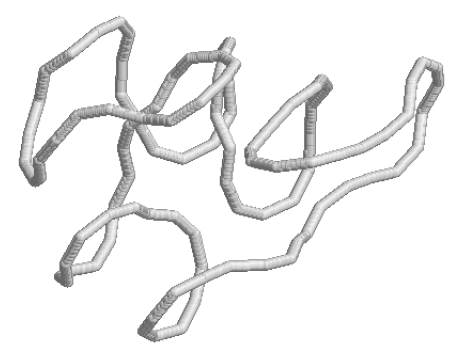
\includegraphics[width=0.471\textwidth,height=0.353\textwidth]{flexibleRing.png}
\end{center}
\caption{Sketch of a flexible ring polymer.}
\label{fig:flexibleRing}
\end{figure}

\begin{align}
P_{1r}(q) & = \sqrt{\frac{2}{u_{1r}^2}} D\left[ \sqrt{\frac{u_{1r}^2}{2}} \right] \\
u_{1r}^2 &= q^2R^2_{g,1r} \\
R^2_{g,1r} &= \sqrt{\frac{b^2N}{12}} \\
D(X) &= \exp\left(X^2\right) \int_0^X \exp(t^2)\, \mathrm{d}t
\end{align}

\vspace{5mm}

\noindent
\underline{Input Parameters for model \texttt{FlexibleRingPolymer}:}
\begin{description}
\item[\texttt{Rg}] radius of gyration $R_G$
\item[\texttt{I0}] forward scattering $I_0$
\end{description}

\begin{figure}[htb]
\begin{center}
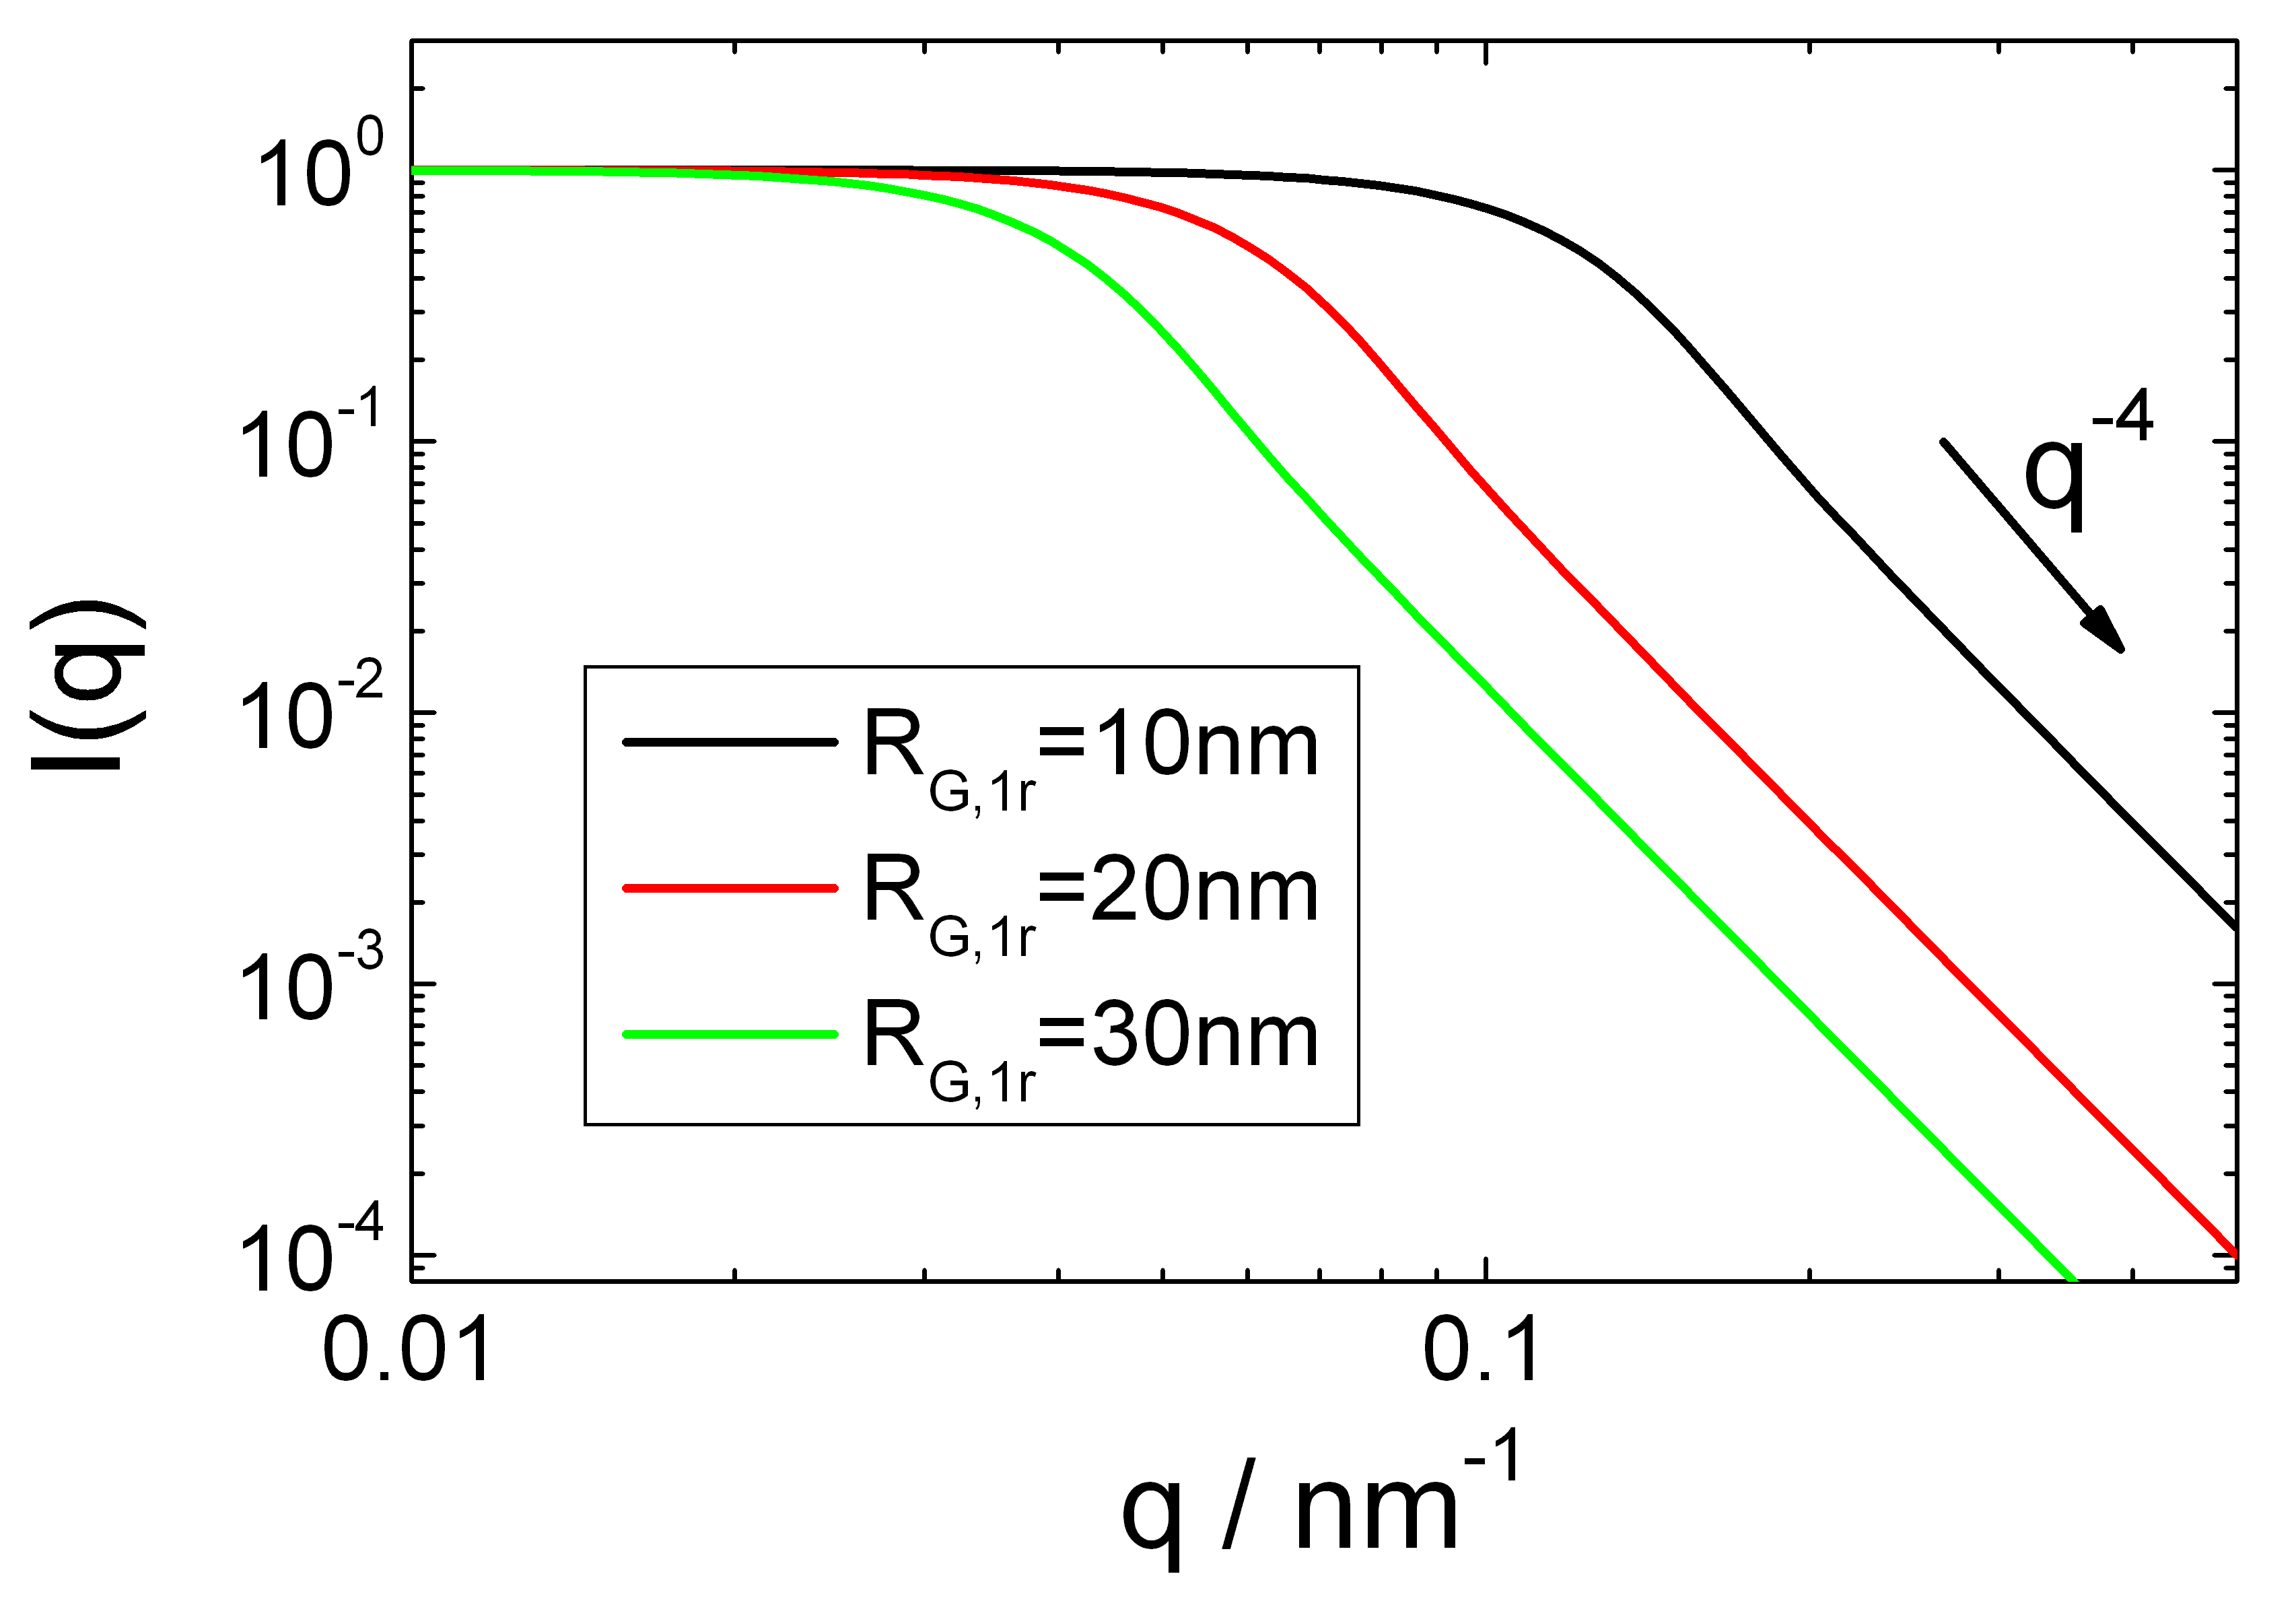
\includegraphics[width=0.768\textwidth,height=0.588\textwidth]{ringIQ.png}
\end{center}
\caption{Scattering intensity of ring polymers of different radius of gyration.} \label{fig:ringIQ}
\end{figure}

%%%%%%%%%%%%%%%%%%%%%%%%%%%%%%%%%%%%%%%%%%%%%%%%%%%%%%%%%%%%%%%%%%%%%%%

\clearpage
\subsection{$m$-membered twisted ring \cite{Burchard1996}}
\label{sect:mMemberedTwistedRing}
~\\
\begin{figure}[htb]
\begin{center}
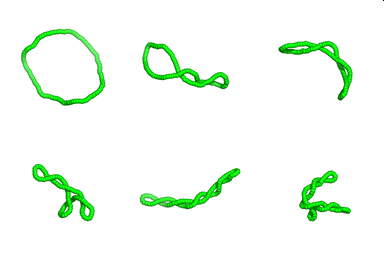
\includegraphics[width=0.768\textwidth,height=0.516\textwidth]{TWsnap.png}
\end{center}
\caption{Sketch of ing polymers which different degree of twisting}
\label{fig:mMemberedTwistedRing}
\end{figure}

\begin{align}
P_{mr}(q) & = I_0\left(\frac{P_{1r}(q)}{m} + \frac{2}{m^2}P_{1r}^2(q)\sum_{j=1}^{m-1}(m-j)\exp\left(-\frac{q^2R^2_{g,1r}}{2}(j-1)\right)\right) \\
P_{1r}(q) & = \sqrt{\frac{2}{u_{1r}^2}} D\left[ \sqrt{\frac{u_{1r}^2}{2}} \right] \\
u_{1r}^2 &= q^2R^2_{g,1r} \\
R^2_{g,1r} &= \sqrt{\frac{b^2N}{12}} \\
D(X) &= \exp\left(X^2\right) \int_0^X \exp(t^2)\, \mathrm{d}t
\end{align}

\vspace{5mm}

\noindent
\underline{Input Parameters for model \texttt{mMemberedTwistedRing}:}
\begin{description}
\item[\texttt{R\_G,1r}] radius of gyration $R_{G,1r}$ of one of $m$ loop
\item[\texttt{m}]  number of twists $m$
\item[\texttt{I0}] forward scattering $I_0$
\end{description}

\begin{figure}[htb]
\begin{center}
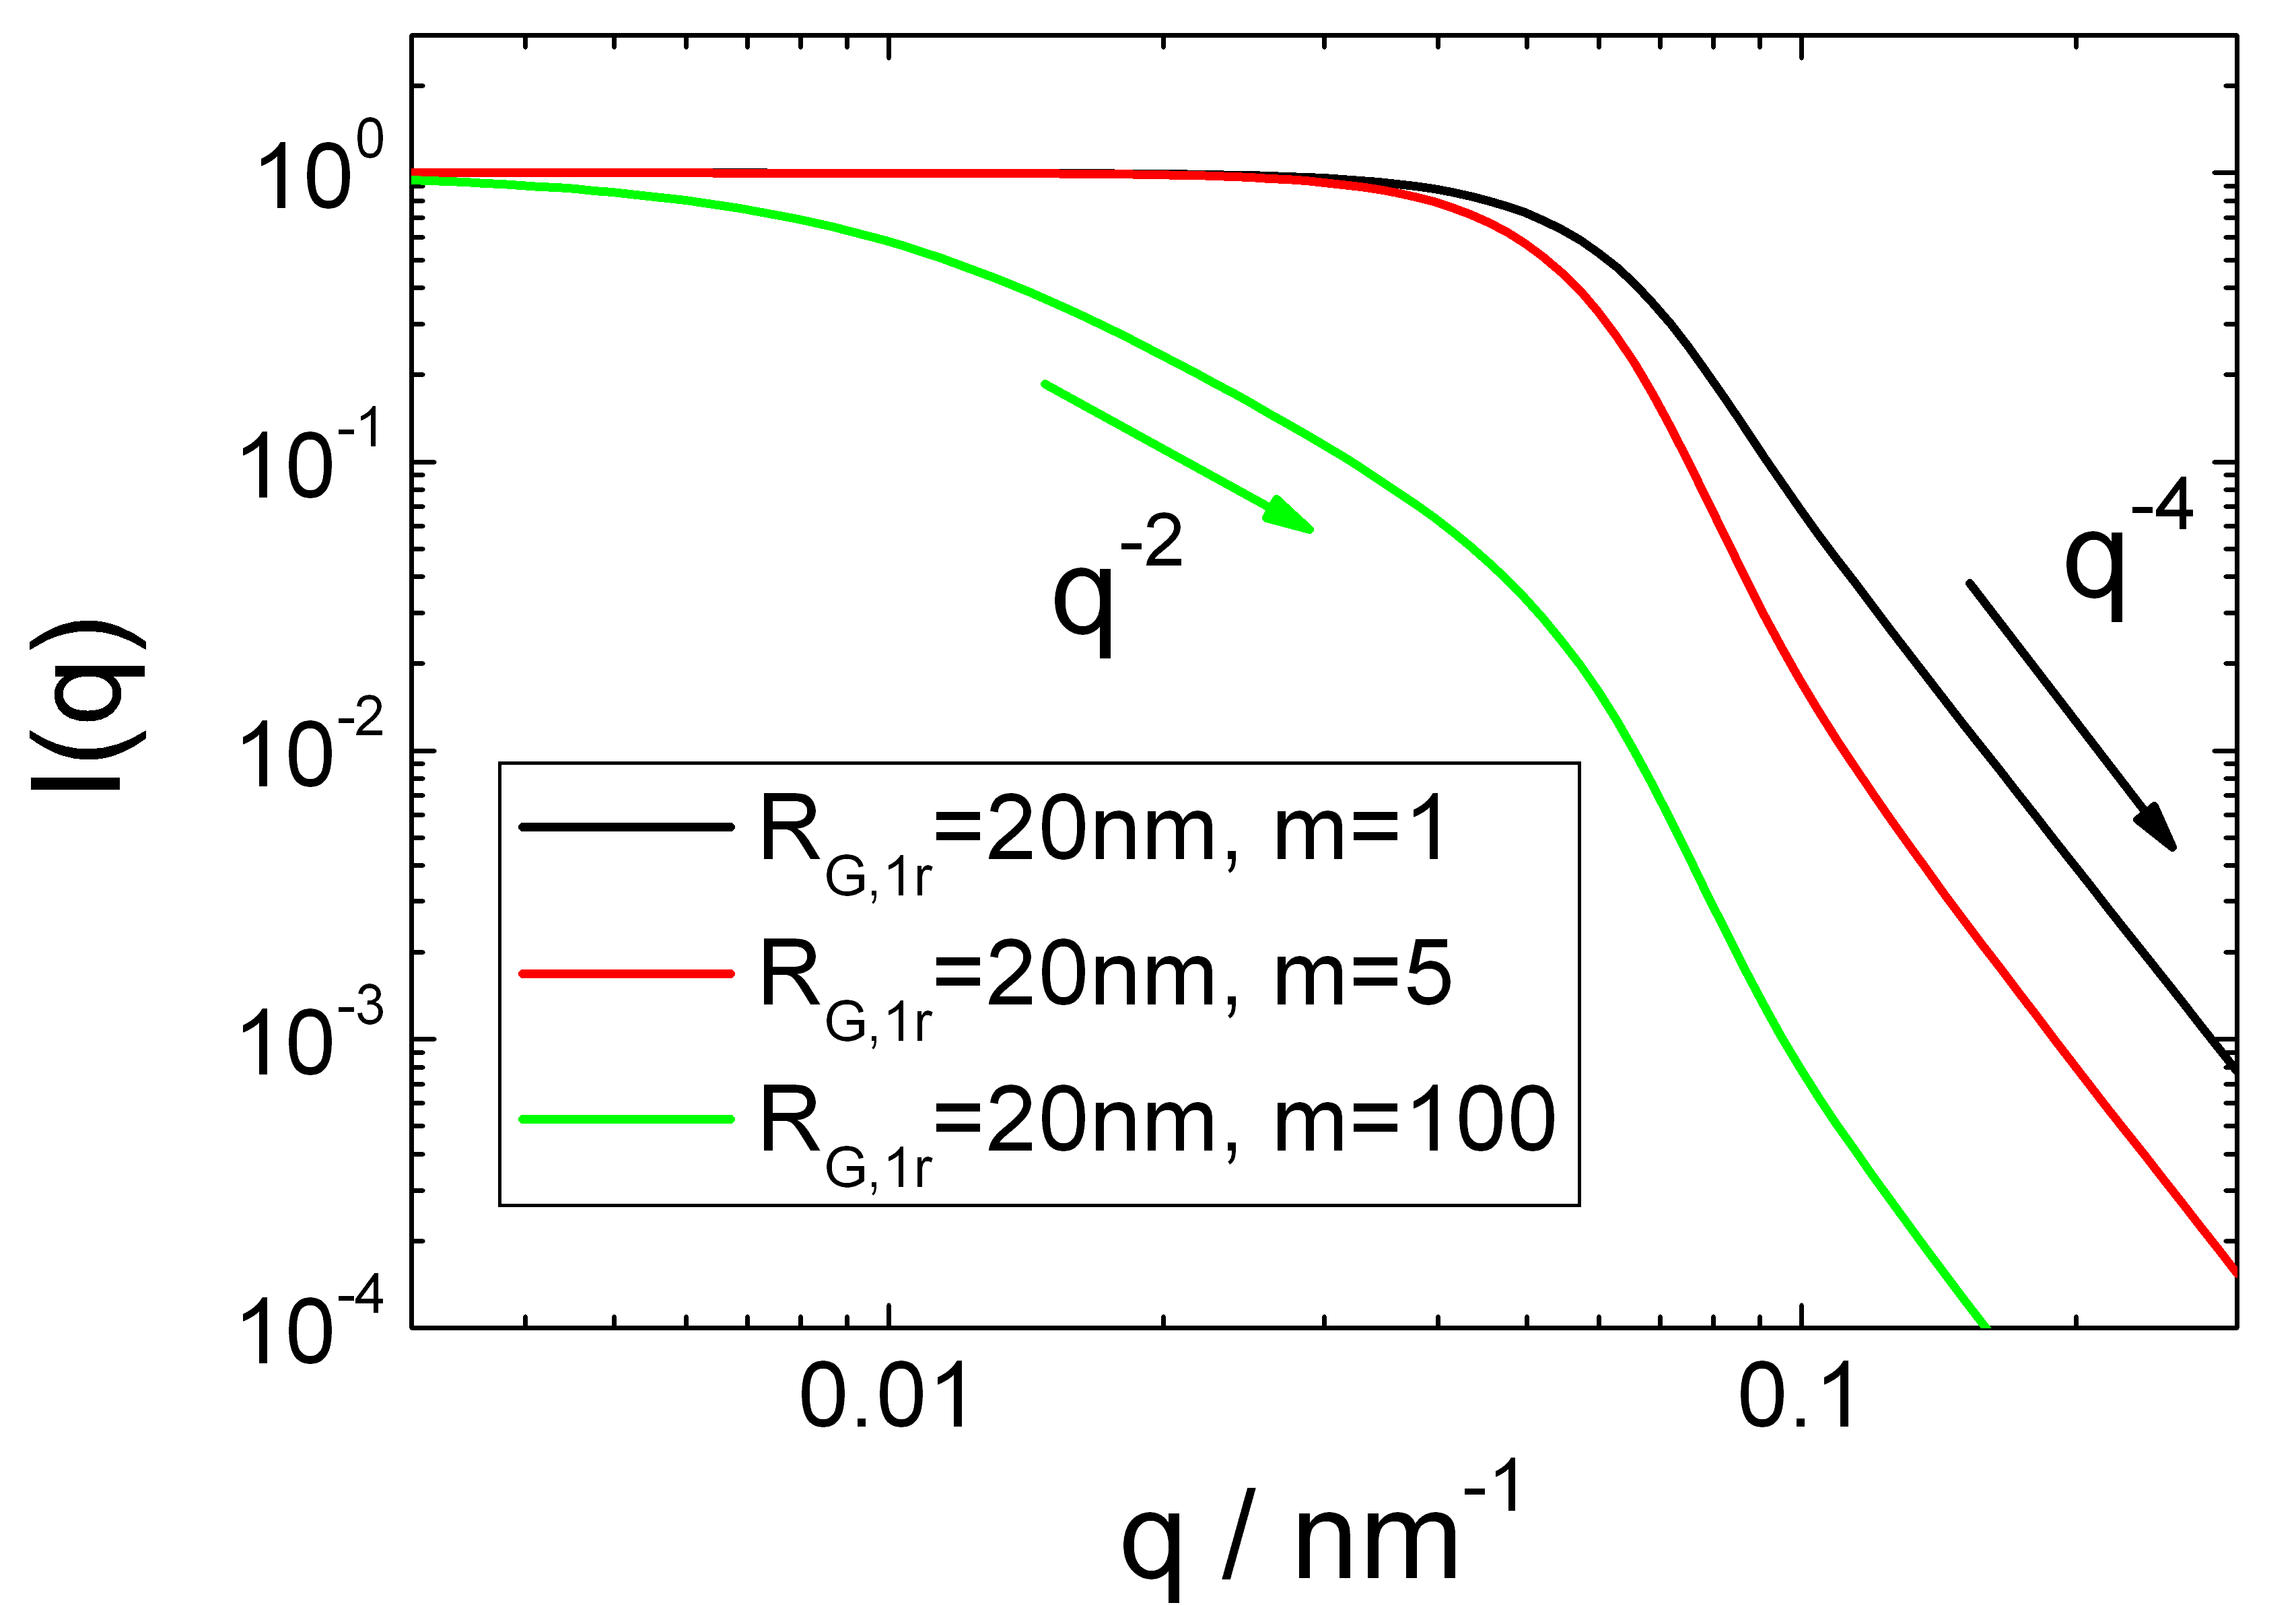
\includegraphics[width=0.768\textwidth,height=0.588\textwidth]{mMemberedTwistedRing.png}
\end{center}
\caption{Scattering intensity of an $m$-membered twisted ring polymers with different values for $m$.} \label{fig:mMemberedTwistedRingIQ}
\end{figure}

%%%%%%%%%%%%%%%%%%%%%%%%%%%%%%%%%%%%%%%%%%%%%%%%%%%%%%%%%%%%%%%%%%%%%%%%

\clearpage
\subsection{Daisy-like Ring \cite{Burchard1996}}
\label{sect:DaisyLikeRing}
~\\
\begin{figure}[htb]
\begin{center}
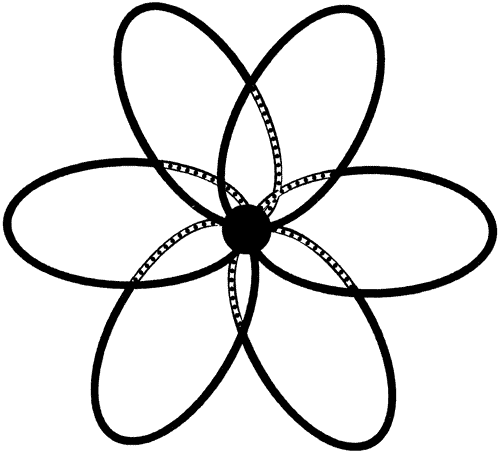
\includegraphics[width=0.5\textwidth,height=0.453\textwidth]{ma9603286f00001.png}
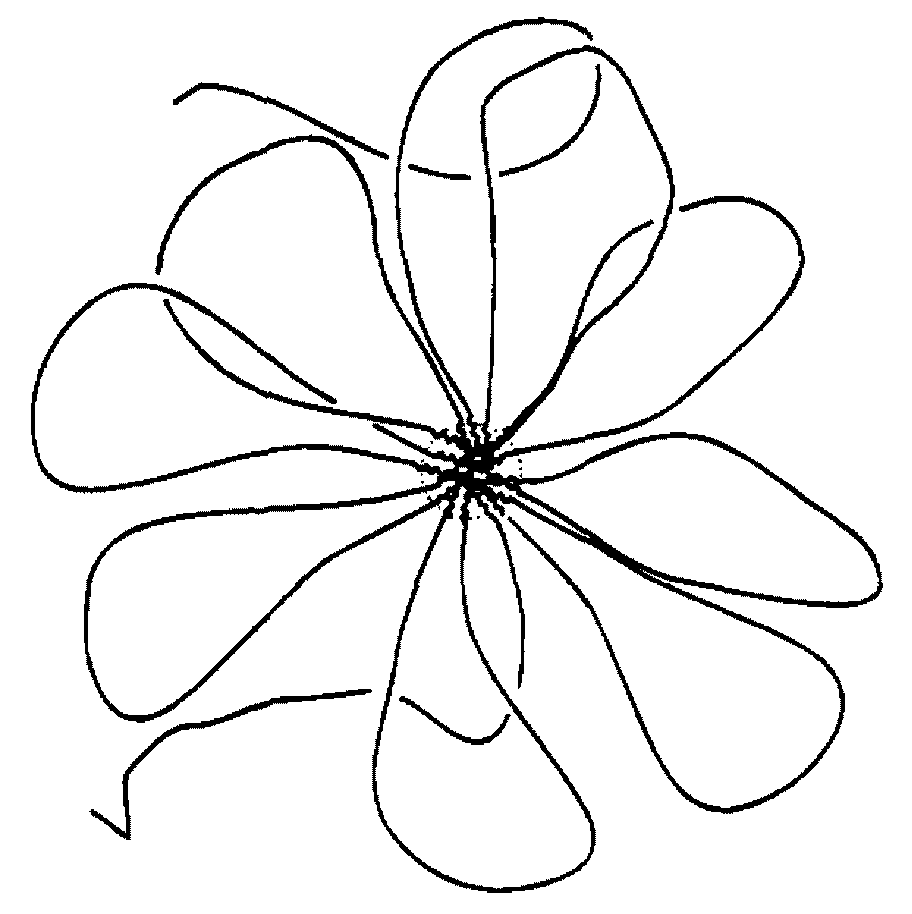
\includegraphics[width=0.45\textwidth,height=0.45\textwidth]{RosetteLikeMicelle.png}
\end{center}
\caption{Sketch of a Daisy-like polymer.}
\label{fig:DaisyLike}
\end{figure}

\begin{align}
P_{mr}(q) & = \frac{I_0}{m}\left(P_{1r}(q) + (m-1)P_{1r}^2(q)\right) \\
P_{1r}(q) & = \sqrt{\frac{2}{u_{1r}^2}} D\left[ \sqrt{\frac{u_{1r}^2}{2}} \right] \\
u_{1r}^2 &= q^2R^2_{g,1r} \\
R^2_{g,1r} &= \sqrt{\frac{b^2N}{12}} \\
D(X) &= exp(X^2) \int_0^X exp(t^2)\, \mathrm{d}t
\end{align}

\vspace{5mm}

\noindent
\underline{Input Parameters for model \texttt{DaisyLikeRing}:}
\begin{description}
\item[\texttt{R\_G,1r}] radius of gyration $R_{G,1r}$ of one of $m$ loop
\item[\texttt{m}]  number of loops $m$
\item[\texttt{I0}] forward scattering $I_0$
\end{description}

\begin{figure}[htb]
\begin{center}
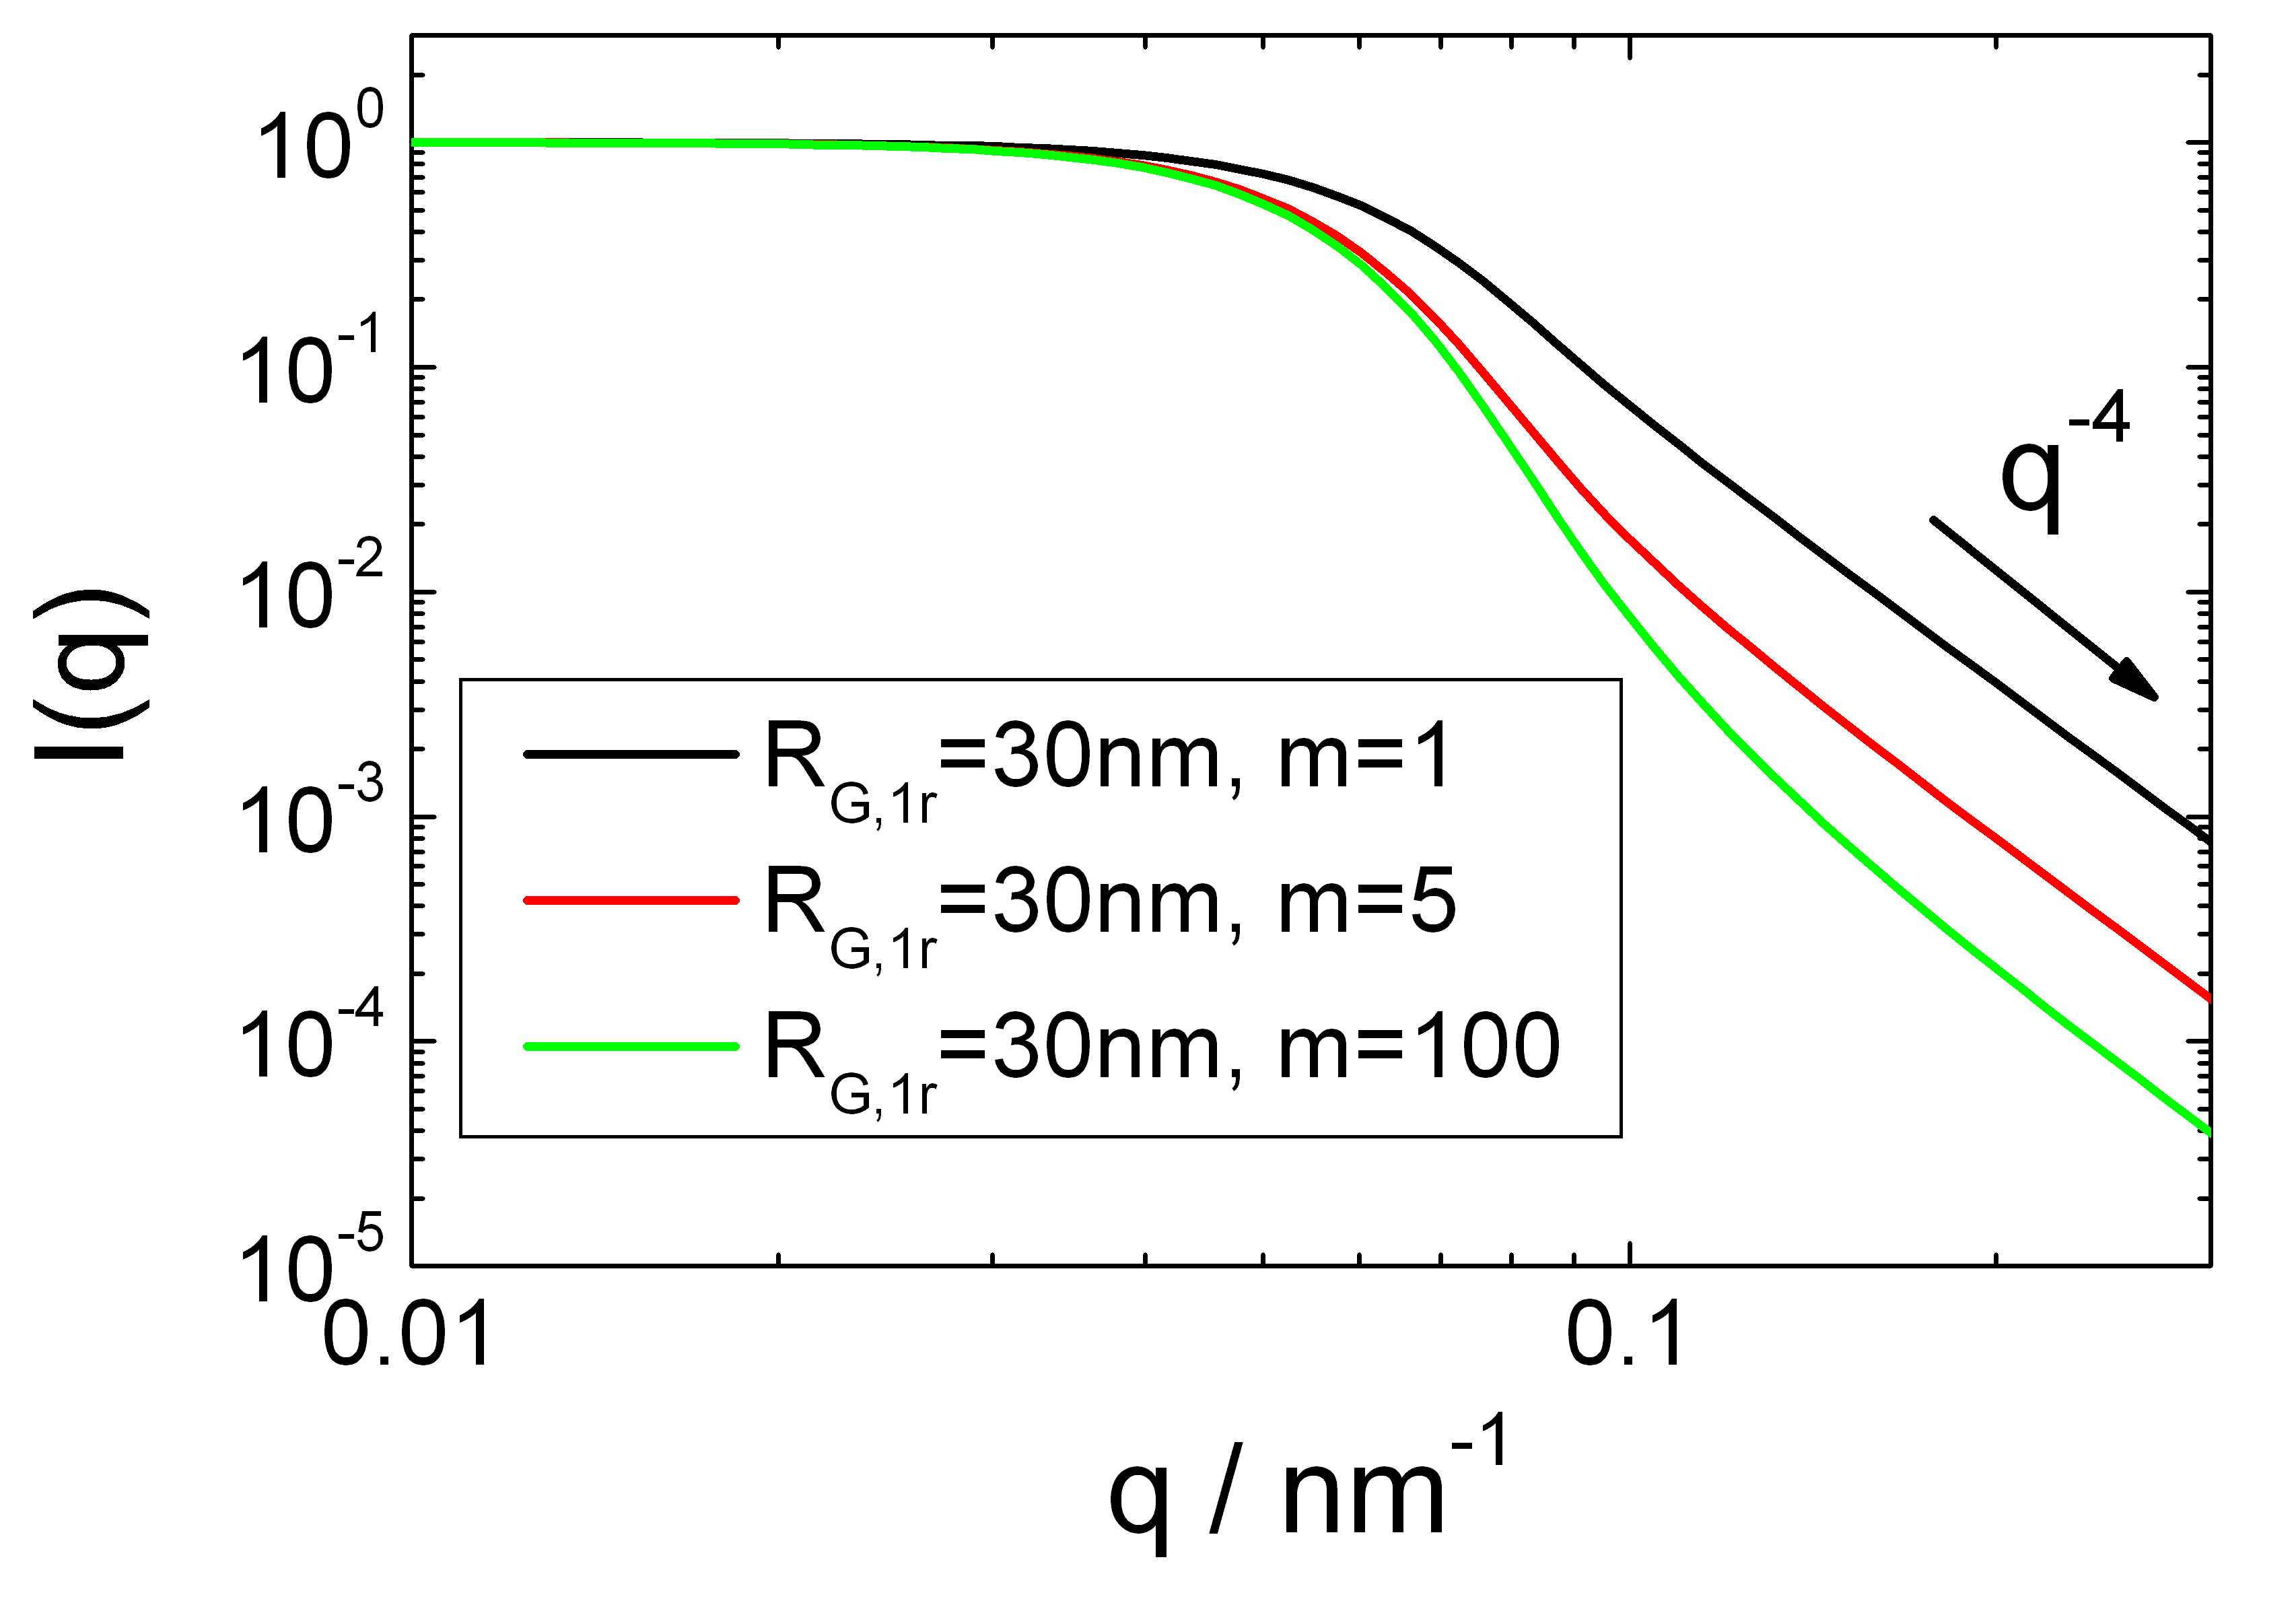
\includegraphics[width=0.768\textwidth,height=0.588\textwidth]{DaisyRingIQ.png}
\end{center}
\caption{Scattering intensity of a Daisy-like ring polymers with different number of loops.} \label{fig:DaisyRingIQ}
\end{figure}
%%%%%%%%%%%%%%%%%%%%%%%%%%%%%%%%%%%%%%%%%%%%%%%%%%%%%%%%%%%%%%%%%%%%%%%

\clearpage

\subsection{Unified Exponential Power Law according to Beaucage \cite{beaucage95,beaucage96}}
\label{sect:Beaucage}
~\\

\begin{figure}[htb]
\begin{center}
\includegraphics[width=0.952\textwidth,height=0.403\textwidth]{Beaucage.png}
\end{center}
\caption{A typical case in which two $R_g$'s are observed.
Particles composed of sub-particles where a radius of gyration for
the entire particle, $R_g$, and a radius of gyration for the
sub-particles, $R_s$, are observed. The surface-fractal cut-off
radius of gyration, $R_{sub}$, differs from the high-$Q$ radius of
gyration, $R_s$, in this case. Generally, $R_s = R_{sub}$}
\label{Beaucage}
\end{figure}

\subsubsection{Beaucage} ~\\

\begin{align}
\begin{split}
I_\text{Beaucage}(Q) & \simeq
    G \exp\left(-\frac{Q^2R_g^2}{3}\right) \\
& + B \exp\left(-\frac{Q^2R_{sub}^2}{3}\right)
      \left( \frac{\left[\mathrm{erf}\left(QkR_g/\sqrt{6}\right)\right]^3}{Q}\right)^P  \\
& + G_s \exp\left(-\frac{Q^2R_s^2}{3}\right) \\
& + B_s %\exp\left(\frac{-Q^2R_{sub}^2}{3}\right)
      \left( \frac{\left[\mathrm{erf}\left(Qk_sR_s/\sqrt{6}\right)\right]^3}{Q}\right)^{P_s}
\end{split} \label{eq:UEPL}
\end{align}
The first term in eq.\ \ref{eq:UEPL} describes the large-scale
structure of size $R_g$ composed of small subunits of
size $R_s$, captured in the third term. The second term describes
the mass-fractal regime with two structural limits. The low-$Q$
limit is at $R_g$ and is described by the error function. The
high-$Q$ limit is at $R_{sub}$ and is described by the exponential
pre-factor \cite{beaucage95} . The final two terms are for the
sub-structural mer unit. Using eq.\ \ref{eq:UEPL}, scattering from a
system with multiple-size-scale features is parameterized.
Generally, the high-$Q$ cutoff for the intermediate power law,
$R_{sub}$, is identical to the sub-structural radius of gyration,
$R_s$. The assumption that $R_{sub} = R_s$ should always be true
for typical mass fractals. It should be noted that, although eq.\
\ref{eq:UEPL} appears cumbersome, no new parameters have been
introduced over local fits using exponentials and power laws.

$G$ is the Guinier pre-factor defined above and $B$ is a
pre-factor specific to the type of power-law scattering:
$B$ is defined according to the regime in which the exponent
$P$ falls. Generally, for surface fractals $4 > P > 3$,
for mass fractals $P < 3$ and for diffuse interfaces $P>4$.
For Porod's law, $P=4$
and $B = N_p 2\pi \rho_c^2pS_p$, where $S_p$, is the particulate surface
area. For a Gaussian polymer, $P = 2$, and $B$ is given by
$2G/R_g^2$, through a comparison with the Debye form factor \ref{sect:GaussCoil}
at the high-$Q$ limit as discussed below.
The constant, $k$ in \ref{eq:UEPL}, accounts for
an approximation involved in the description of the low-$Q$
power-law limit \cite{beaucage95}. This is an empirical
constant that has a value of 1 for steep power-law decays,
$P > 3$. For weak power-law decays, $k$ deviates slightly
from 1. For polymeric mass fractals of fractal dimension
$d_f$ close to 2 (1.5 to 3), $k$ is empirically found to be close
to 1.06. Weak deviations are observed between the scattered
intensity as calculated using \ref{eq:UEPL} and exact
calculations for values of $Q$ between $2\pi/R_g$ and $\pi/R_g$ in
these cases when $k = 1$. These deviations are reduced to
less than 3\% of the calculated intensity using $k= 1.06$.

\hspace{1pt}\\
\underline{Input Parameters for model \texttt{Beaucage}:}\\
\begin{description}
\item[\texttt{G}] $G$ is the Guinier pre-factor of the larger structure
\item[\texttt{B}] $B$ is a pre-factor specific to the type of power-law scattering:
$B$ is defined according to the regime in which the exponent $P$ falls.
\item[\texttt{Gs}] $G_s$ is the Guinier pre-factor of the smaller structure
\item[\texttt{Bs}] $B_s$ is a pre-factor specific to the type of power-law scattering:
$B_s$ is defined according to the regime in which the exponent $P_s$ falls.
\item[\texttt{Rg}] large-scale structure
\item[\texttt{Rsub}] surface-fractal cut-off radius of gyration,
$R_{sub}$ defines the high-$Q$ cutoff for the intermediate power law
\item[\texttt{Rs}] size $R_s$ of small subunits
\item[\texttt{P}] scaling exponent of the power law assigned to the larger structure $R_g$
\item[\texttt{Ps}] scaling exponent of the power law assigned to the smaller structure $R_s$
\end{description}


\begin{figure}[htb]
\begin{center}
\includegraphics[width=0.75\textwidth,height=0.5\textwidth]{../images/form_factor/nonparticular/Beaucage.png}
\end{center}
\caption{}
\label{fig:Beaucage}
\end{figure}

\clearpage
\subsubsection{Beaucage2} ~\\

Equation \ref{eq:UEPL} can be extended to describe an arbitrary
number of interrelated structural levels under the
generally applicable assumption that $R_\text{sub} = R_s$,
\begin{align}
\begin{split}
I_\text{Beaucage}(Q)  \simeq \sum_{i=1}^n & G_i \exp\left(-\frac{Q^2R_{g,i}^2}{3}\right) \\
 + & B_i \exp\left(-\frac{Q^2R_{g,i+1}^2}{3}\right)
      \left( \frac{\left[\mathrm{erf}\left(Qk_iR_{g,i}/\sqrt{6}\right)\right]^3}{Q}\right)^{P_i}
\end{split}
\label{eq:generalizedUEPL}
\end{align}
In \ref{eq:generalizedUEPL}, $i= 1$ refers to the largest-size structural level.
Extensions, such as eq.\ \ref{eq:generalizedUEPL}, can only be justified when data
extend over many decades in $Q$. Eq.\ \ref{eq:generalizedUEPL} introduces no
new parameters over local Guinier and power-law fits.


\hspace{1pt}\\
\underline{Input Parameters for model \texttt{Beaucage2}:}\\
\begin{description}
\item[\texttt{G}] Guinier pre-factor $G_i$
\item[\texttt{B}] pre-factor $B_i$, specific to the type of power-law scattering:
$B_i$ is defined according to the regime in which the exponent $P_i$ falls.
\item[\texttt{R\_i}] large-scale structure $R_{g,i}$
\item[\texttt{R\_i+1}] size $R_{g,i+1}$ of smaller subunits
\item[\texttt{k}] This is an empirical constant that has a value of 1 for steep power-law decays,
$P > 3$. For weak power-law decays, $k$ deviates slightly from 1
\item[\texttt{P}] scaling exponent of the power law assigned to the larger structure $R_{g,i}$
\end{description}
\noindent\underline{Note:}
For calculating a summation over $n$ interrelated structural levels one has to use global fitting. For \texttt{R\_i} and \texttt{R\_i+1} one has to define global parameters, let say P1 and P2 in the first scattering contribution. In the second scattering contribution one has to use for \texttt{R\_i} the same global parameter P2 as for \texttt{R\_i+1} in the previous scattering contribution. The global parameters for \texttt{R\_i} in one scattering contribution and the global parameter for \texttt{R\_i+1} in the previous scattering contribution have to be the same. By this an arbitrary number of interrelated structural levels can be calculated.

\begin{figure}[htb]
\begin{center}
\includegraphics[width=0.75\textwidth,height=0.5\textwidth]{../images/form_factor/nonparticular/Beaucage2.png}
\end{center}
\caption{}
\label{fig:Beaucage2}
\end{figure}

%\noindent REFERENCE:\\
%G. Beaucage, Approximations Leading to a Unified
%Exponential/Power-Law Approach to Small-Angle Scattering, J. Appl.
%Cryst. (1995). 28, 717-728 \\
%G. Beaucage, Small-Angle Scattering from Polymeric Mass Fractals
%of Arbitrary Mass-Fractal Dimension,  J. Appl. Crystallogr. , 29,
%134-146 (1996).

%%%%%%%%%%%%%%%%%%%%%%%%%%%%%%%%%%%%%%%%%%%%%%%%%%%%%%%%%%%%%%%%%%%%%%%%%

\clearpage
\subsection{WormLikeChainEXV \cite{Pedersen96Macrom}}
\label{sect:WormLikeChain}
~\\
\begin{figure}[htb]
\begin{center}
\includegraphics[width=0.8\textwidth,height=0.4\textwidth]{wormlike2.png}
\end{center}
\caption{The chain of contour length, $L$, (the total length) can
be described a chain of some number of locally stiff segments of
length $l_p$. The persistence length,$l_p$, is the length along
the cylinder over which the flexible cylinder can be considered a
rigid rod. The Kuhn length ($b$) used in the model is also used to
describe the stiffness of a chain, and is simply $b = 2l_p$.}
\label{wormlike2}
\end{figure}

This form factor calculates the form factor for a flexible
cylinder with a circular cross section and a uniform scattering
length density. The non-negligible diameter of the cylinder is
included by accounting for excluded volume interactions within the
walk of a single cylinder. Inter-cylinder interactions are NOT
included. The function calculated has been given by Pedersen et al.\
\cite{Pedersen96Macrom}. The model "Method 3 With Excluded Volume" is used,
which is a parametrization of simulations of a discrete
representation of the worm-like chain model of Kratky and Porod
applied in the pseudo-continuous limit.

\vspace{5mm}

\hspace{1pt}\\
\underline{Input Parameters for model \texttt{WormLikeChainEXV}:}\\
\begin{description}
\item[\texttt{R}] radius $R$ of cylindrical core with uniform scattering length density
\item[\texttt{l}] Kuhn length\footnote{The Kuhn length $l$ is related to the length $a$ of
    locally stiff segment simply via $l=2a$} $l$ of semi-flexible worm-like structure
\item[\texttt{L}] contour length $L$ of semi-flexible worm-like structure
\end{description}

\begin{figure}[htb]
\begin{center}
\includegraphics[width=0.768\textwidth,height=0.588\textwidth]{wormlike_Iq.png}
\end{center}
\caption{Comparison of wormlike micelles according to Pedersen \cite{Pedersen96Macrom}
and Kholodenko \cite{kholodenko93}} \label{fig:wormlike_Iq}
\end{figure}


%%%%%%%%%%%%%%%%%%%%%%%%%%%%%%%%%%%%%%%%%%%%%%%%%%%%%%%%%%%%%%%%%%%%%%%%%

\clearpage
\subsection{KholodenkoWorm}
\label{sect:KholodenkoWorm}~\\

\begin{figure}[htb]
\begin{center}
\includegraphics[width=0.617\textwidth,height=0.762\textwidth]{SemiflexiblePolymerTxt.png}
\end{center}
\caption{}
\label{fig:KholodenkoWorm}
\end{figure}

Kholodenko \cite{kholodenko93} presented a new approach using the analogy between Dirac�s fermions
and semi-flexible polymers. The form factor $P_0(Q)$ resulting
from Kholodenko�s approach is designed to reproduce
correctly the rigid-rod limit and the random-coil limit.
Defining $x = 3L/l$ ($L$: contour length, $l$: Kuhn length), it is given by
\begin{align}
P_0(Q,L,l) &= \frac{2}{x} \left[I_{(1)} -\frac{1}{x}I_{(2)}\right]
\label{eq:Kholodenko}
\end{align}
where
\begin{align}
I_{(n)}(x) &= \int_0^x  f(z) \, z^{n-1} \, dz
\end{align}
together with
\begin{align}
f(z)) &=
\begin{cases} \displaystyle
\frac{1}{E}\frac{\sinh(Ez)}{\sinh(z)} & \text{for} \quad \displaystyle Q \leq \frac{3}{l}\\ \\
\displaystyle
\frac{1}{F}\frac{\sin(Fz)}{\sinh(z)} & \text{for} \quad \displaystyle Q > \frac{3}{l}
\end{cases}
\end{align}
and
\begin{align}
E = \sqrt{1-\left(\frac{lQ}{3}\right)^2} \quad \text{and} \quad F = \sqrt{\left(\frac{lQ}{3}\right)^2-1}
\end{align}

For flexible cylinders with a circular cross section and a uniform scattering
length density the cross section form factor is given by
\begin{align}
P_{cs} = \left(2 \frac{J_1(QR)}{QR}\right)^2
\end{align}
so that the overall form factor is given by
\begin{align}
P(Q,L,l,R) = P_0(Q,L,l)\, P_{cs}(Q,R)
\end{align}

\vspace{5mm}

\hspace{1pt}\\
\underline{Input Parameters for model \texttt{KholodenkoWorm}:}\\
\begin{description}
\item[\texttt{R}] radius $R$ of cylindrical core with uniform scattering length density
\item[\texttt{l}] Kuhn length\footnote{The Kuhn length $l$ is related to the length $a$ of
    locally stiff segment simply via $l=2a$} $l$ of semi-flexible worm-like structure
\item[\texttt{L}] contour length $L$ of semi-flexible worm-like structure
\end{description}

\begin{figure}[htb]
\begin{center}
\includegraphics[width=0.768\textwidth,height=0.588\textwidth]{wormlike_Iq.png}
\end{center}
\caption{Comparison of wormlike micelles according to Pedersen \cite{Pedersen96Macrom}
and Kholodenko \cite{kholodenko93}. } \label{fig:wormlike_Iq2}
\end{figure}

%%%%%%%%%%%%%%%%%%%%%%%%%%%%%%%%%%%%%%%%%%%%%%%%%%%%%%%%%%%%%%%%%%%%%%%%%
\clearpage

\subsection{Diblock copolymer micelles}
\label{subsect:DiblockCopolymerMicelles}
~\\
\begin{figure}[htb]
\centering
  \subfigure[spherical
  micelle]{\quad\includegraphics[width=0.25\textwidth,height=0.375\textwidth]{spheregauss.png}\quad}
  \quad
  \subfigure[ellipsoidal
  micelle]{\quad\includegraphics[width=0.25\textwidth,height=0.41\textwidth]{ellipsoidgauss.png}\quad}
  \quad
  \subfigure[cylindrical micelle]{\quad\includegraphics[width=0.2\textwidth,height=0.4\textwidth]{cylindergauss.png}\quad}
  \caption{Block copolymer forming micelles of different shapes}
\end{figure}

For block copolymers, which form micelles, several form factor have
been implemented \cite{PedersenGerstenberg96,PedersenJApplCryst2000,SvaneborgPedersen2002}
for spherical, ellipsoidal, and cylindrical shapes.
It has been assumed that one unit is forming the core of the
micelles and the other the corona. The core is assumed to have a
homogeneous scattering length density, but may contain some amount
of solvent. For the polymer chains in the corona either a model
where Gaussian chains are attached to the core or a corona model of
semi-flexible interacting self-avoiding chains (only for spherical
core) or a continuous model, where a radial profile of the form
$\Phi(r)\varpropto r^{-\alpha}$ has been assumed. The form factors
have been parameterized such, that the excess scattering of the
corona and the core are consistent with the composition and density
of the two separate block units of the copolymer.

\vspace{3mm}
\subsubsection{Micelles with a homogeneous core and Gaussian chains on the surface}
\label{Chains(RW)} ~\\
%\phantomsection
%\addcontentsline{toc}{subsubsection}{\indexname}
%\printindex

It is assumed that the diblock copolymer consist of a block unit for
which the solvent is poor and a block unit with is good. The
insoluble blocks form a relatively compact core whereas the soluble
blocks form a diffuse corona surrounding the core. The form factor
of a micelle contains four different terms: the self-correlation
term of the core $N_\text{agg}^2\beta_\text{core}^2\,P_\text{core}(q)$,
the self-correlation term of the chains
$N_\text{agg}\beta_\text{brush}^2\,P_\text{brush}(q)$, the cross-term
between the core and chains
$2N_\text{agg}^2\beta_\text{core}\beta_\text{brush}\,S_\text{brush-core}(q)$,
and the cross term between different chains
$N_\text{agg}(N_\text{agg}-1)\beta_\text{brush}^2\,S_\text{brush-brush}(q)$.
It can be written (Pedersen \& Gerstenberg, 1996)
\begin{align}
I_\text{mic}    &= N_\text{agg}^2\beta_\text{core}^2\,P_\text{core}(q) + N_\text{agg}\beta_\text{brush}^2\,P_\text{brush}(q)  \label{eq:micelle}\\
                &+ 2N_\text{agg}^2\beta_\text{core}\beta_\text{brush}\,S_\text{brush-core}(q) + N_\text{agg}(N_\text{agg}-1)\beta_\text{brush}^2\,S_\text{brush-brush}(q)\nonumber
\end{align}
$N_\text{agg}$ is the aggregation number of diblock polymers forming
the micelle and $\beta_\text{brush}=V_\text{brush}(\eta_\text{brush}-\eta_\text{solv})$
and $\beta_\text{core}=V_\text{core}(\eta_\text{core}-\eta_\text{solv})$
the excess scattering length of a block in the corona and in the core, respectively.
$V_\text{brush}$ and $V_\text{core}$ are the total volume of a block in the corona
and in the core. $\eta_\text{brush}$ and $\eta_\text{core}$ are the corresponding
scattering length densities and $\eta_\text{solv}$ is the scattering length
density of the surrounding solvent. The functions $P_\text{core}(q)$, $P_\text{brush}(q)$,
$S_\text{brush-core}(q)$, and $S_\text{brush-brush}(q)$ are all 1 for $q=0$. The definitions
of these four functions depend on the shape of the core and are given below.

\vspace{5mm}

\subsubsection{\bf Spherical core:} \label{sect:SphericalMicelles}
\vspace{5mm}
\begin{align}
P_\text{core}(q,R_\text{core}) &= \Phi^2(qR_\text{core}) \\
\Phi(qR) &= 3\frac{\sin(qR)-qR\cos(qR)}{(qR)^3}
\end{align}
\begin{align}
P_\text{brush}(q,R_g)&= 2\frac{\exp(-x)-1+x}{x^2} \text{~with~} x = R_g^2q^2
\end{align}
\begin{align}
S_\text{brush-core}(q,R_\text{core},Rg,d) &= \Phi(qR_\text{core})\psi(qR_g)\frac{\sin(q[R_\text{core}+dR_g])}{q[R_\text{core}+dR_g]} \\
\psi(qRg) &= \frac{1-\exp(-x)}{x} \text{~(form factor amplitude of the chain)} \nonumber
\end{align}
\begin{align}
S_\text{brush-brush}(q,R_\text{core},d,R_g) &= \psi^2(qR_g)\left[\frac{\sin(q[R_\text{core}+dR_g])}{q[R_\text{core}+dR_g]}\right]^2
\end{align}

\vspace{5mm}

For micelles with a spherical core a few different parameterizations have been
implemented \texttt{SPHERE+Chains(RW)}, \texttt{SPHERE+Chains(RW)\_Rc} and
\texttt{SPHERE+Chains(RW)\_Nagg}.
The parameters they all have in common are:
\begin{description}
\item[$V_\text{brush}$] molecular volume the diblock copolymer part forming the corona
\item[$\eta_\text{core}$] scattering length density of the diblock copolymer part forming the core
\item[$\eta_\text{brush}$] scattering length density of the diblock copolymer part forming the corona
\item[$\eta_\text{solv}$] scattering length density of the solvent
\item[$x_\text{solv,core}$] volume fraction of solvent in the micellar core
\item[$R_g$] radius of gyration of the block unit in the corona
\item[$d$]  non-penetration of the chains into the core is mimicked by
$d\sim 1$ for $R_\text{core}\gg R_g$
\end{description}

\vspace{10mm}

\noindent
For the model \texttt{SPHERE+Chains(RW)} the other parameters are
\begin{description}
\item[$R_\text{core}$] radius of the micellar core
\item[$n_\text{agg}$] grafting density (number of copolymer molecules
$N_\text{agg}$ per surface are $S$, $n_\text{agg}=N_\text{agg}/S$)
\end{description}

\noindent
In contrast to the form factor \texttt{SPHERE+Chains(RW)\_Rc} and \texttt{SPHERE+Chains(RW)\_Nagg}
this one does not necessary consist of copolymers.
The excess scattering lengths and aggregation number needed in eq.\
\ref{eq:micelle} are than given by
\begin{align}
N_\text{agg} &= n_\text{agg} S
\end{align}
where the surface of the core is given by $S=4\pi R_\text{core}^2$. Together with the
core volume  $V =\frac{4}{3}\pi R_\text{core}^3$ one gets for the excess scattering
lengths
\begin{align}
\beta_\text{core} &= \frac{V (1-x_\text{solv,core})}{N_\text{agg}}
(\eta_\text{core}-\eta_\text{solv}) \\
\beta_\text{brush} &= V_\text{brush} (\eta_\text{brush}-\eta_\text{solv})
\end{align}

\vspace{3mm}

\hspace{1pt}\\
\underline{Input Parameters for model \texttt{SPHERE+Chains(RW)}:}\\
\begin{description}
\item[\texttt{R\_core}] core radius
\item[\texttt{n\_agg}] specific aggregation number (number of chains per surface area)
\item[\texttt{V\_brush}]  molecular volume of a block unit in the micellar corona
\item[\texttt{eta\_core}] scattering length density of spherical core
\item[\texttt{eta\_brush}] scattering length density of the block unit in the corona
\item[\texttt{eta\_solv}] scattering length density of solvent
\item[\texttt{xsolv\_core}] amount of solvent in core
\item[\texttt{Rg}] gyration radius of polymer chains in the corona
\item[\texttt{d}] This value should be around 1. Non-penetration of the chains
into the core is mimicked by $d\sim 1$ for $R_\text{core}\gg R_g$
\end{description}

\vspace{10mm}

\noindent
For the model \texttt{SPHERE+Chains(RW)\_Rc} the other parameters are
\begin{description}
\item[$R_\text{core}$] core radius
\item[$V_\text{core}$] molecular volume of single block unit in the micellar core
\end{description}
The excess scattering lengths and aggregation number in eq.\
\ref{eq:micelle} are given by
\begin{align}
\beta_\text{core}  &= V_\text{core}  (\eta_\text{core} -\eta_\text{solv}) \\
\beta_\text{brush} &= V_\text{brush} (\eta_\text{brush}-\eta_\text{solv}) \\
N_\text{agg} &= (1-x_\text{solv,core}) \frac{4}{3}\pi R_\text{core}^3  / V_\text{core}
\end{align}

\hspace{1pt}\\
\underline{Input Parameters for model \texttt{SPHERE+Chains(RW)\_Rc}:}
\begin{description}
\item[\texttt{R\_core}] core radius
\item[\texttt{V\_core}] molecular volume of single block unit in the micellar core
\item[\texttt{V\_brush}]  molecular volume of single block unit in the micellar corona
\item[\texttt{eta\_core}] scattering length density of spherical core
\item[\texttt{eta\_brush}] scattering length density of the block unit in the corona
\item[\texttt{eta\_solv}] scattering length density of solvent
\item[\texttt{xsolv\_core}] amount of solvent in core
\item[\texttt{Rg}] gyration radius of polymer chains in the corona
\item[\texttt{d}] This value should be around 1. Non-penetration of the chains
into the core is mimicked by $d\sim 1$ for $R_\text{core}\gg R_g$
\end{description}

\vspace{10mm}

\noindent
For the model \texttt{SPHERE+Chains(RW)\_Nagg} the other parameters are
\begin{description}
\item[$N_\text{agg}$] aggregation number
\item[$V_\text{core}$] molecular volume of single block unit in the micellar core
\end{description}
The excess scattering lengths and the core radius $R_\text{core}$ needed in eq.\
\ref{eq:micelle} are given by
\begin{align}
\beta_\text{core}  &= V_\text{core}  (\eta_\text{core} -\eta_\text{solv}) \\
\beta_\text{brush} &= V_\text{brush} (\eta_\text{brush}-\eta_\text{solv}) \\
R_\text{core} &= \left( \frac{N_\text{agg} V_\text{core}}{1-x_\text{solv,core}}
                         \, \frac{3}{4\pi}\right)^{1/3}
\end{align}

\hspace{1pt}\\
\underline{Input Parameters for model \texttt{SPHERE+Chains(RW)\_Nagg}:}
\begin{description}
\item[\texttt{N\_agg}] aggregation number
\item[\texttt{V\_core}] molecular volume of single block unit in the micellar core
\item[\texttt{V\_brush}]  molecular volume of single block unit in the micellar corona
\item[\texttt{eta\_core}] scattering length density of spherical core
\item[\texttt{eta\_brush}] scattering length density of the block unit in the corona
\item[\texttt{eta\_solv}] scattering length density of solvent
\item[\texttt{xsolv\_core}] amount of solvent in core
\item[\texttt{Rg}] gyration radius of polymer chains in the corona
\item[\texttt{d}] This value should be around 1. Non-penetration of the chains
into the core is mimicked by $d\sim 1$ for $R_\text{core}\gg R_g$
\end{description}

\clearpage \noindent \subsubsection{\bf ellipsoidal core with
semi-axis $(R,R,\epsilon R)$:} \label{sect:ELLMicelles}
\vspace{5mm}
\begin{align}
P_\text{core}(q,R_\text{core},\epsilon) &= \int_0^{\pi/2}\Phi^2[qr(R_\text{core},\epsilon,\alpha)] \, \sin\alpha \, d\alpha \\
\text{with~} \, r(R_\text{core},\epsilon,\alpha) &= R_\text{core}\sqrt{\sin^2\alpha+\epsilon^2\cos^2\alpha} \nonumber
\end{align}
\begin{align}
P_\text{brush}(q,R_g)&= 2\frac{\exp(-x)-1+x}{x^2} \text{~with~} x = R_g^2q^2
\end{align}
\begin{align}
S_\text{brush-core}(q,R_\text{core},\epsilon,Rg,d) &=
        \psi(qR_g)\int_0^{\pi/2} \Phi(qr(\dots))\frac{\sin(q[r(\dots)+dR_g])}{q[r(\dots)+dR_g]} \, \sin\alpha \, d\alpha
\end{align}
\begin{align}
S_\text{brush-brush}(q,R_\text{core},d,R_g) &= \psi^2(qR_g) \int_0^{\pi/2}\left[\frac{\sin(q[r(\dots)+dR_g])}{q[r(\dots)+dR_g]}\right]^2 \, \sin\alpha \, d\alpha
\end{align}

\noindent
As for micelles with spherical core also for those with an ellipsoidal core several
parameterizations have been implemented \texttt{ELL+Chains(RW)}, \texttt{ELL+Chains(RW)\_Rc} and
\texttt{ELL+Chains(RW)\_Nagg}. \sloppy
The parameters they all have in common are:
\begin{description}
\item[$V_\text{brush}$] molecular volume the diblock copolymer part forming the corona
\item[$\eta_\text{core}$] scattering length density of the diblock copolymer part forming the core
\item[$\eta_\text{brush}$] scattering length density of the diblock copolymer part forming the corona
\item[$\eta_\text{solv}$] scattering length density of the solvent
\item[$x_\text{solv,core}$] volume fraction of solvent in the micellar core
\item[$R_g$] radius of gyration of the block unit in the corona
\item[$d$]  non-penetration of the chains into the core is mimicked by
$d\sim 1$ for $R_\text{core}\gg R_g$
\item[$\epsilon$] eccentricity of the ellipsoidal micelle $(R_\text{core},R_\text{core},\epsilon R_\text{core})$
\end{description}

\vspace{10mm}

\noindent
For the model \texttt{ELL+Chains(RW)} the other parameters are
\begin{description}
\item[$R_\text{core}$] radius of the micellar core $(R_\text{core},R_\text{core},\epsilon R_\text{core})$
\item[$n_\text{agg}$] grafting density (number of copolymer molecules
$N_\text{agg}$ per surface are $S$, $n_\text{agg}=N_\text{agg}/S$)
\end{description}

\noindent
In contrast to the form factor \texttt{ELL+Chains(RW)\_Rc} and \texttt{ELL+Chains(RW)\_Nagg}
this one does not necessary consist of copolymers.
The excess scattering lengths and aggregation number needed in eq.\
\ref{eq:micelle} are given by \sloppy
\begin{align}
N_\text{agg} &= n_\text{agg} S
\end{align}
where the surface of the core is given by
\begin{align}
S  &=
\begin{cases}
 2\pi R_\text{core}^2 \left(1+\frac{\text{arctanh}(\sin({\ae}))}{\sin({\ae})}\right)& \text{for~} \epsilon < 1 \\
 2\pi R_\text{core}^2 \left(1+\frac{\ae}{\tan({\ae})}\right) & \text{for~} \epsilon \geq 1
\end{cases} \\
{\ae} &=
\begin{cases}
 \arccos(\epsilon) & \text{for~} \epsilon < 1 \\
 \arccos(1/\epsilon) & \text{for~} \epsilon \geq 1
\end{cases} \nonumber
\end{align}
Together with the core volume
$V =\frac{4}{3}\pi \epsilon R_\text{core}^3$ one gets for the excess scattering
lengths
\begin{align}
\beta_\text{core} &= \frac{V (1-x_\text{solv,core})}{N_\text{agg}}
(\eta_\text{core}-\eta_\text{solv}) \\
\beta_\text{brush} &= V_\text{brush} (\eta_\text{brush}-\eta_\text{solv})
\end{align}

\vspace{3mm}

\hspace{1pt}\\
\underline{Input Parameters for model \texttt{ELL+Chains(RW)}:}\\
\begin{description}
\item[\texttt{R\_core}] core radius
\item[\texttt{n\_agg}] specific aggregation number (number of chains per surface area)
\item[\texttt{V\_brush}]  molecular volume of a block unit in the micellar corona
\item[\texttt{eta\_core}] scattering length density of spherical core
\item[\texttt{eta\_brush}] scattering length density of the block unit in the corona
\item[\texttt{eta\_solv}] scattering length density of solvent
\item[\texttt{xsolv\_core}] amount of solvent in core
\item[\texttt{Rg}] gyration radius of polymer chains in the corona
\item[\texttt{d}] This value should be around 1. Non-penetration of the chains
into the core is mimicked by $d\sim 1$ for $R_\text{core}\gg R_g$
\item[\texttt{epsilon}] eccentricity of the ellipsoidal micelle
$(R_\text{core},R_\text{core},\epsilon R_\text{core})$
\end{description}

\vspace{10mm}

\noindent
For the model \texttt{ELL+Chains(RW)\_Rc} the other parameters are
\begin{description}
\item[$R_\text{core}$] core radius
\item[$V_\text{core}$] molecular volume of single block unit in the micellar core
\end{description}
The excess scattering lengths and aggregation number in eq.\
\ref{eq:micelle} are given by
\begin{align}
\beta_\text{core}  &= V_\text{core}  (\eta_\text{core} -\eta_\text{solv}) \\
\beta_\text{brush} &= V_\text{brush} (\eta_\text{brush}-\eta_\text{solv}) \\
N_\text{agg} &= (1-x_\text{solv,core}) \frac{4}{3}\pi \epsilon R_\text{core}^3  / V_\text{core}
\end{align}
\underline{Input Parameters for model \texttt{ELL+Chains(RW)\_Rc}:}
\begin{description}
\item[\texttt{R\_core}] core radius
\item[\texttt{V\_core}] molecular volume of single block unit in the micellar core
\item[\texttt{V\_brush}]  molecular volume of single block unit in the micellar corona
\item[\texttt{eta\_core}] scattering length density of spherical core
\item[\texttt{eta\_brush}] scattering length density of the block unit in the corona
\item[\texttt{eta\_solv}] scattering length density of solvent
\item[\texttt{xsolv\_core}] amount of solvent in core
\item[\texttt{Rg}] gyration radius of polymer chains in the corona
\item[\texttt{d}] This value should be around 1. Non-penetration of the chains
into the core is mimicked by $d\sim 1$ for $R_\text{core}\gg R_g$
\item[\texttt{epsilon}] eccentricity of the ellipsoidal micelle
$(R_\text{core},R_\text{core},\epsilon R_\text{core})$
\end{description}

\vspace{5mm}

\noindent
For the model \texttt{ELL+Chains(RW)\_Nagg} the other parameters are
\begin{description}
\item[$N_\text{agg}$] aggregation number
\item[$V_\text{core}$] molecular volume of single block unit in the micellar core
\end{description}
The excess scattering lengths and the core radius $R_\text{core}$ needed in eq.\
\ref{eq:micelle} are given by
\begin{align}
\beta_\text{core}  &= V_\text{core}  (\eta_\text{core} -\eta_\text{solv}) \\
\beta_\text{brush} &= V_\text{brush} (\eta_\text{brush}-\eta_\text{solv}) \\
R_\text{core} &= \left( \frac{N_\text{agg} V_\text{core}}{1-x_\text{solv,core}}
                        \, \frac{3}{4\pi\epsilon}\right)^{1/3}
\end{align}
\underline{Input Parameters for model \texttt{ELL+Chains(RW)\_Nagg}:}
\begin{description}
\item[\texttt{N\_agg}] aggregation number
\item[\texttt{V\_core}] molecular volume of single block unit in the micellar core
\item[\texttt{V\_brush}]  molecular volume of single block unit in the micellar corona
\item[\texttt{eta\_core}] scattering length density of spherical core
\item[\texttt{eta\_brush}] scattering length density of the block unit in the corona
\item[\texttt{eta\_solv}] scattering length density of solvent
\item[\texttt{xsolv\_core}] amount of solvent in core
\item[\texttt{Rg}] gyration radius of polymer chains in the corona
\item[\texttt{d}] This value should be around 1. Non-penetration of the chains
into the core is mimicked by $d\sim 1$ for $R_\text{core}\gg R_g$
\item[\texttt{epsilon}] eccentricity of the ellipsoidal micelle
$(R_\text{core},R_\text{core},\epsilon R_\text{core})$
\end{description}


\clearpage
\noindent
\subsubsection{\bf cylindrical core with radius $R_\text{core}$ and height $H$:}
\label{sect:CylMicelles}
~\\
\begin{align}
P_\text{core}(q,R_\text{core},H) &= \int_0^{\pi/2}\Psi^2(q,R_\text{core},H,\alpha) \, \sin\alpha \, d\alpha \\
\text{with~} \, \Psi(q,R_\text{core},H,\alpha) &=
    \frac{2J_1(qR_\text{core}\sin\alpha)}{qR_\text{core}\sin\alpha}
    \frac{\sin(qH/2\, \cos\alpha)}{qH/2\, \cos\alpha}
\end{align}
and $J_1(x)$ is the first order Bessel function of the first kind.
\begin{align}
P_\text{brush}(q,R_g)&= 2\frac{\exp(-x)-1+x}{x^2} \text{~with~} x = R_g^2q^2
\end{align}
\begin{align}
S_\text{brush-core}(q,& R_\text{core},H,Rg,d) = \psi(qR_g) \quad \times \\
   & \int_0^{\pi/2} \Psi(q,R_\text{core},H,\alpha) \Xi(q,R+dR_g,H+2dR_g,\alpha) \, \sin\alpha \, d\alpha \nonumber
\end{align}
where $\Xi(q,R_\text{core},H,\alpha)$ is the form factor amplitude of the shell:
\begin{align}
\Xi(q, R_\text{core} H,\alpha)  &= \biggl[ \frac{R}{R_\text{core}+H} \frac{2J_1(qR_\text{core}\sin\alpha)}{qR_\text{core}\sin\alpha} \cos(qH/2\, \cos\alpha) \\
                                &+ \frac{H}{R_\text{core}+H} J_0(qR_\text{core}\sin\alpha) \frac{\sin(qH/2\, \cos\alpha)}{qH/2\, \cos\alpha} \biggr] \nonumber
\end{align}
where $J_0(x)$ is the zeroth order Bessel function of the first kind.
\begin{align}
S_\text{brush-brush}(q,& R_\text{core},H,d,R_g) = \psi^2(qR_g) \quad \times \\
 &\int_0^{\pi/2} \Xi^2(q,R_\text{core}+dR_g,H+2dR_g,\alpha)\, \sin\alpha \, d\alpha \nonumber
\end{align}

\noindent
As for micelles with spherical core also for those with a cylindrical core several
parameterizations have been implemented \texttt{CYL+Chains(RW)}, \texttt{CYL+Chains(RW)\_Rc} and
\texttt{CYL+Chains(RW)\_Nagg}.
The parameters they all have in common are: \sloppy
\begin{description}
\item[$V_\text{brush}$] molecular volume the diblock copolymer part forming the corona
\item[$\eta_\text{core}$] scattering length density of the diblock copolymer part forming the core
\item[$\eta_\text{brush}$] scattering length density of the diblock copolymer part forming the corona
\item[$\eta_\text{solv}$] scattering length density of the solvent
\item[$x_\text{solv,core}$] volume fraction of solvent in the micellar core
\item[$R_g$] radius of gyration of the block unit in the corona
\item[$d$]  non-penetration of the chains into the core is mimicked by
$d\sim 1$ for $R_\text{core}\gg R_g$
\item[$H$] height of the cylindrical core of the micelle
\end{description}


\vspace{10mm}

\noindent
For the model \texttt{CYL+Chains(RW)} the other parameters are
\begin{description}
\item[$R_\text{core}$] radius of the micellar core $(R_\text{core},R_\text{core},\epsilon R_\text{core})$
\item[$n_\text{agg}$] grafting density (number of copolymer molecules
$N_\text{agg}$ per surface are $S$, $n_\text{agg}=N_\text{agg}/S$)
\end{description}

\noindent
In contrast to the form factor \texttt{CYL+Chains(RW)\_Rc} and \texttt{CYL+Chains(RW)\_Nagg}
this one does not necessary consist of copolymers.
The excess scattering lengths and aggregation number needed in eq.\
\ref{eq:micelle} are than given by
\begin{align}
N_\text{agg} &= n_\text{agg} S
\end{align}
where the surface of the core is given by
\begin{align}
S  &= 2\pi R_\text{core} H
\end{align}
Together with the core volume $V =\pi R_\text{core}^2 H$
one can calculate the excess scattering lengths by
\begin{align}
\beta_\text{core} &= \frac{V (1-x_\text{solv,core})}{N_\text{agg}}
(\eta_\text{core}-\eta_\text{solv}) \\
\beta_\text{brush} &= V_\text{brush} (\eta_\text{brush}-\eta_\text{solv})
\end{align}

\hspace{1pt}\\
\underline{Input Parameters for model \texttt{CYL+Chains(RW)}:}
\begin{description}
\item[\texttt{R\_core}] core radius
\item[\texttt{n\_agg}] specific aggregation number (number of chains per surface area)
\item[\texttt{V\_brush}]  molecular volume of a block unit in the micellar corona
\item[\texttt{eta\_core}] scattering length density of spherical core
\item[\texttt{eta\_brush}] scattering length density of the block unit in the corona
\item[\texttt{eta\_solv}] scattering length density of solvent
\item[\texttt{xsolv\_core}] amount of solvent in core
\item[\texttt{Rg}] gyration radius of polymer chains in the corona
\item[\texttt{d}] This value should be around 1. Non-penetration of the chains
into the core is mimicked by $d\sim 1$ for $R_\text{core}\gg R_g$
\item[\texttt{H}] height of the cylindrical core of the micelle
\end{description}

\vspace{10mm}

\noindent
For the model \texttt{CYL+Chains(RW)\_Rc} the other parameters are
\begin{description}
\item[$R_\text{core}$] core radius
\item[$V_\text{core}$] molecular volume of single block unit in the micellar core
\end{description}
The excess scattering lengths and aggregation number in eq.\
\ref{eq:micelle} are than given by
\begin{align}
\beta_\text{core}  &= V_\text{core}  (\eta_\text{core} -\eta_\text{solv}) \\
\beta_\text{brush} &= V_\text{brush} (\eta_\text{brush}-\eta_\text{solv}) \\
N_\text{agg} &= (1-x_\text{solv,core}) \pi  R_\text{core}^2 H  / V_\text{core}
\end{align}

\hspace{1pt}\\
\underline{Input Parameters for model \texttt{CYL+Chains(RW)\_Rc}:}
\begin{description}
\item[\texttt{R\_core}] core radius
\item[\texttt{V\_core}] molecular volume of single block unit in the micellar core
\item[\texttt{V\_brush}]  molecular volume of single block unit in the micellar corona
\item[\texttt{eta\_core}] scattering length density of spherical core
\item[\texttt{eta\_brush}] scattering length density of the block unit in the corona
\item[\texttt{eta\_solv}] scattering length density of solvent
\item[\texttt{xsolv\_core}] amount of solvent in core
\item[\texttt{Rg}] gyration radius of polymer chains in the corona
\item[\texttt{d}] This value should be around 1. Non-penetration of the chains
into the core is mimicked by $d\sim 1$ for $R_\text{core}\gg R_g$
\item[\texttt{H}] height of the cylindrical core of the micelle
\end{description}

\vspace{3mm}

\noindent
For the model \texttt{CYL+Chains(RW)\_Nagg} the other parameters are
\begin{description}
\item[$N_\text{agg}$] aggregation number
\item[$V_\text{core}$] molecular volume of single block unit in the micellar core
\end{description}
The excess scattering lengths and the core radius $R_\text{core}$ are given by
\begin{align}
\beta_\text{core}  &= V_\text{core}  (\eta_\text{core} -\eta_\text{solv}) \\
\beta_\text{brush} &= V_\text{brush} (\eta_\text{brush}-\eta_\text{solv}) \\
R_\text{core} &= \sqrt{ \frac{N_\text{agg} V_\text{core}}{1-x_\text{solv,core}}
                \, \frac{1}{\pi H}}
\end{align}


\hspace{1pt}\\
\underline{Input Parameters for model \texttt{CYL+Chains(RW)\_Nagg}:}
\begin{description}
\item[\texttt{N\_agg}] aggregation number
\item[\texttt{V\_core}] molecular volume of single block unit in the micellar core
\item[\texttt{V\_brush}]  molecular volume of single block unit in the micellar corona
\item[\texttt{eta\_core}] scattering length density of spherical core
\item[\texttt{eta\_brush}] scattering length density of the block unit in the corona
\item[\texttt{eta\_solv}] scattering length density of solvent
\item[\texttt{xsolv\_core}] amount of solvent in core
\item[\texttt{Rg}] gyration radius of polymer chains in the corona
\item[\texttt{d}] This value should be around 1. Non-penetration of the chains
into the core is mimicked by $d\sim 1$ for $R_\text{core}\gg R_g$
\item[\texttt{H}] height of the cylindrical core of the micelle
\end{description}


\clearpage
\noindent
\subsubsection{\bf wormlike micelles with cylindrical cross-section with radius $R_\text{core}$,
Kuhn-length $l$ and contour length  $L$:}
\label{sect:WormLikeMicelles}
~\\
The form factors for a worm-like micelles are approximated by the form factor of the Kholodenko-worm
according to section \ref{sect:KholodenkoWorm} where the scattering length density profile across the worm segments are
described by those of a rod-like micelle \ref{sect:RodLikeMicelles}.
The corresponding function in eq.\ \ref{eq:micelle} are given by
\begin{align}
P_\text{core}(q,R_\text{core},l,L) &= P_\text{worm}(q,l,L) P_\text{cs}(q,R_\text{core},d,R_g)
\label{eq:wormlikeFF}
\end{align}
the contributiion of the worm-like conformation of the micelle $P_\text{worm}(q,l,L)$ is described
by the formula of Kholodenko for worm-like structures given in eq.\ \ref{eq:Kholodenko}.
The contribution of the cross-section $P_\text{cs}$ is the same as for rod-like micelles and
given by
\begin{align}
P_\text{cs}(q,R_\text{core},d,R_g) &= \left[ \frac{2J_1(qR_\text{core})}{qR_\text{core}} \right]^2 \\
\text{Si}(x) &= \int_0^x \, t^{-1} \sin t\, dt
\end{align}
\begin{align}
P_\text{brush}(q,R_g)&= 2\frac{\exp(-x)-1+x}{x^2} \text{~with~} x = R_g^2q^2
\end{align}
\begin{align}
S_\text{brush-core}(q,& R_\text{core},l,L,Rg,d) = \psi(qR_g) \quad \times \\
                           & \frac{2J_1(qR_\text{core})}{qR_\text{core}}
                            J_0[q(r_\text{core}+dR_g)]  P_\text{worm}(q,l,L) \nonumber
\end{align}
\begin{align}
S_\text{brush-brush}(q,R_\text{core},l,L,d,R_g) &=
\psi^2(qR_g) J_0^2[q(r_\text{core}+dR_g)]  P_\text{worm}(q,l,L)
\end{align}

\vspace{1cm}

\noindent
As for micelles with spherical core also for those worm-like micelles several
parameterizations have been implemented \texttt{WORM+Chains(RW)}, \texttt{WORM+Chains(RW)\_Rc} and
\texttt{WORM+Chains(RW)\_nagg}.
The parameters they all have in common are: \sloppy
\begin{description}
\item[$V_\text{brush}$] molecular volume the diblock copolymer part forming the corona
\item[$\eta_\text{core}$] scattering length density of the diblock copolymer part forming the core
\item[$\eta_\text{brush}$] scattering length density of the diblock copolymer part forming the corona
\item[$\eta_\text{solv}$] scattering length density of the solvent
\item[$x_\text{solv,core}$] volume fraction of solvent in the micellar core
\item[$R_g$] radius of gyration of the block unit in the corona
\item[$l$] contour length of the worm-like of the micelle
\item[$L$] contour length of the worm-like of the micelle
\end{description}


\vspace{10mm}

\noindent
For the model \texttt{WORM+Chains(RW)} the other parameters are
\begin{description}
\item[$R_\text{core}$] radius of the micellar core
\item[$n_\text{agg}$] grafting density (number of copolymer molecules
$N_\text{agg}$ per surface are $S$, $n_\text{agg}=N_\text{agg}/S$)
\end{description}

\noindent
In contrast to the form factor \texttt{WORM+Chains(RW)\_Rc} and \texttt{WORM+Chains(RW)\_nagg}
this one does not necessary consist of copolymers.
The excess scattering lengths and aggregation number needed in eq.\
\ref{eq:micelle} are than given by
\begin{align}
N_\text{agg} &= n_\text{agg} S
\end{align}
where the surface of the core is given by
\begin{align}
S  &= 2\pi R_\text{core} L
\end{align}
Together with the core volume $V =\pi R_\text{core}^2 L$
one can calculate the excess scattering lengths by
\begin{align}
\beta_\text{core} &= \frac{V (1-x_\text{solv,core})}{N_\text{agg}}
(\eta_\text{core}-\eta_\text{solv}) \\
\beta_\text{brush} &= V_\text{brush} (\eta_\text{brush}-\eta_\text{solv})
\end{align}

\hspace{1pt}\\
\underline{Input Parameters for model \texttt{WORM+Chains(RW)}:}
\begin{description}
\item[\texttt{R\_core}] core radius
\item[\texttt{n\_agg}] specific aggregation number (number of chains per surface area)
\item[\texttt{V\_brush}]  molecular volume of a block unit in the micellar corona
\item[\texttt{eta\_core}] scattering length density of spherical core
\item[\texttt{eta\_brush}] scattering length density of the block unit in the corona
\item[\texttt{eta\_solv}] scattering length density of solvent
\item[\texttt{xsolv\_core}] amount of solvent in core
\item[\texttt{Rg}] gyration radius of polymer chains in the corona
\item[\texttt{l}] contour length of the worm-like of the micelle
\item[\texttt{L}] contour length of the worm-like of the micelle
\end{description}

\vspace{10mm}

\noindent
For the model \texttt{WORM+Chains(RW)\_Rc} the other parameters are
\begin{description}
\item[$R_\text{core}$] core radius
\item[$V_\text{core}$] molecular volume of single block unit in the micellar core
\end{description}
The excess scattering lengths and aggregation number in eq.\
\ref{eq:micelle} are than given by
\begin{align}
\beta_\text{core}  &= V_\text{core}  (\eta_\text{core} -\eta_\text{solv}) \\
\beta_\text{brush} &= V_\text{brush} (\eta_\text{brush}-\eta_\text{solv}) \\
N_\text{agg} &= (1-x_\text{solv,core}) \pi  R_\text{core}^2 L  / V_\text{core}
\end{align}

\hspace{1pt}\\
\underline{Input Parameters for model \texttt{CYL+Chains(RW)\_Rc}:}
\begin{description}
\item[\texttt{R\_core}] core radius
\item[\texttt{V\_core}] molecular volume of single block unit in the micellar core
\item[\texttt{V\_brush}]  molecular volume of single block unit in the micellar corona
\item[\texttt{eta\_core}] scattering length density of spherical core
\item[\texttt{eta\_brush}] scattering length density of the block unit in the corona
\item[\texttt{eta\_solv}] scattering length density of solvent
\item[\texttt{xsolv\_core}] amount of solvent in core
\item[\texttt{Rg}] gyration radius of polymer chains in the corona
\item[\texttt{l}] contour length of the worm-like of the micelle
\item[\texttt{L}] contour length of the worm-like of the micelle
\end{description}

\vspace{10mm}

\noindent
For the model \texttt{WORM+Chains(RW)\_Nagg} the other parameters are
\begin{description}
\item[$N_\text{agg}$] aggregation number
\item[$V_\text{core}$] molecular volume of single block unit in the micellar core
\end{description}
The excess scattering lengths and the core radius $R_\text{core}$ are given by
\begin{align}
\beta_\text{core}  &= V_\text{core}  (\eta_\text{core} -\eta_\text{solv}) \\
\beta_\text{brush} &= V_\text{brush} (\eta_\text{brush}-\eta_\text{solv}) \\
R_\text{core} &= \sqrt{ \frac{N_\text{agg} V_\text{core}}{1-x_\text{solv,core}}
                \, \frac{1}{\pi L}}
\end{align}


\hspace{1pt}\\
\underline{Input Parameters for model \texttt{CYL+Chains(RW)\_Nagg}:}
\begin{description}
\item[\texttt{N\_agg}] aggregation number
\item[\texttt{V\_core}] molecular volume of single block unit in the micellar core
\item[\texttt{V\_brush}]  molecular volume of single block unit in the micellar corona
\item[\texttt{eta\_core}] scattering length density of spherical core
\item[\texttt{eta\_brush}] scattering length density of the block unit in the corona
\item[\texttt{eta\_solv}] scattering length density of solvent
\item[\texttt{xsolv\_core}] amount of solvent in core
\item[\texttt{Rg}] gyration radius of polymer chains in the corona
\item[\texttt{l}] contour length of the worm-like of the micelle
\item[\texttt{L}] contour length of the worm-like of the micelle
\end{description}



\clearpage
\noindent
\subsubsection{\bf micelles with rod-like core:}
\label{sect:RodLikeMicelles}
~\\
The form factors for micelles with a rod-like core are an approximations of the form factors of micelles
with a cylindrical core where $H\gg R_\text{core}+d R_g$. The corresponding function in
eq.\ \ref{eq:micelle} are given by
\begin{align}
P_\text{core}(q,R_\text{core},H) &= P_H(q,H) P_\text{cs}(q,R_\text{core},d,R_g)
\label{eq:rodlikeFF}
\end{align}
with
\begin{align}
P_H(q,H)    &= 2\text{Si}(qH)/(qH) - 4 \sin^2(qH/2)/(q^2H^2) \\
P_\text{cs}(q,R_\text{core},d,R_g) &= \left[ \frac{2J_1(qR_\text{core})}{qR_\text{core}} \right]^2 \\
\text{Si}(x) &= \int_0^x \, t^{-1} \sin t\, dt
\end{align}
\begin{align}
P_\text{brush}(q,R_g)&= 2\frac{\exp(-x)-1+x}{x^2} \text{~with~} x = R_g^2q^2
\end{align}
\begin{align}
S_\text{brush-core}(q,& R_\text{core},H,Rg,d) = \psi(qR_g) \quad \times \\
                           & \frac{2J_1(qR_\text{core})}{qR_\text{core}}
                            J_0[q(r_\text{core}+dR_g)] P_H(q,H) \nonumber
\end{align}
\begin{align}
S_\text{brush-brush}(q,R_\text{core},H,d,R_g) &=
\psi^2(qR_g) J_0^2[q(r_\text{core}+dR_g)] P_H(q,H)
\end{align}

\vspace{1cm}

\noindent
As otherwise the definitions of the geometry for rod-like micelles are mainly the same
than for cylindrical micelles only the list of input parameters are given here. There is
only one difference in the model \texttt{ROD+Chains(RW)\_Nagg} compared to the
model \texttt{CYL+Chains(RW)\_Nagg} and that is that for rod-like structures always the
grafting density of polymer chains on the surface of the core is used, i.e.
$n_\text{agg}=N_\text{agg}/S$ instead of $N_\text{agg}$. For the model \texttt{ROD+Chains(RW)\_nagg}
this means that the core radius has to be calculated by
$R_\text{core} = 2 n_\text{agg} V_\text{core} / (1-x_\text{solv,core})$

\vspace{3mm}

\underline{Input Parameters for model \texttt{ROD+Chains(RW)}:}\\
\begin{description}
\item[\texttt{R\_core}] core radius
\item[\texttt{n\_agg}] specific aggregation number (number of chains per surface area)
\item[\texttt{V\_brush}]  molecular volume of a block unit in the micellar corona
\item[\texttt{eta\_core}] scattering length density of spherical core
\item[\texttt{eta\_brush}] scattering length density of the block unit in the corona
\item[\texttt{eta\_solv}] scattering length density of solvent
\item[\texttt{xsolv\_core}] amount of solvent in core
\item[\texttt{Rg}] gyration radius of polymer chains in the corona
\item[\texttt{d}] This value should be around 1. Non-penetration of the chains
into the core is mimicked by $d\sim 1$ for $R_\text{core}\gg R_g$
\item[\texttt{H}] height of the rod-like core of the micelle
\end{description}


\vspace{10mm}

\hspace{1pt}\\
\underline{Input Parameters for model \texttt{ROD+Chains(RW)\_Rc}:}\\
\begin{description}
\item[\texttt{R\_core}] core radius
\item[\texttt{V\_core}] molecular volume of single block unit in the micellar core
\item[\texttt{V\_brush}]  molecular volume of single block unit in the micellar corona
\item[\texttt{eta\_core}] scattering length density of spherical core
\item[\texttt{eta\_brush}] scattering length density of the block unit in the corona
\item[\texttt{eta\_solv}] scattering length density of solvent
\item[\texttt{xsolv\_core}] amount of solvent in core
\item[\texttt{Rg}] gyration radius of polymer chains in the corona
\item[\texttt{d}] This value should be around 1. Non-penetration of the chains
into the core is mimicked by $d\sim 1$ for $R_\text{core}\gg R_g$
\item[\texttt{H}] height of the rod-like core of the micelle
\end{description}


\vspace{3mm}

\hspace{1pt}\\
\underline{Input Parameters for model \texttt{ROD+Chains(RW)\_nagg}:} \\
\begin{description}
\item[\texttt{n\_agg}] specific aggregation number (number of chains per surface area)
\item[\texttt{V\_core}] molecular volume of single block unit in the micellar core
\item[\texttt{V\_brush}]  molecular volume of single block unit in the micellar corona
\item[\texttt{eta\_core}] scattering length density of spherical core
\item[\texttt{eta\_brush}] scattering length density of the block unit in the corona
\item[\texttt{eta\_solv}] scattering length density of solvent
\item[\texttt{xsolv\_core}] amount of solvent in core
\item[\texttt{Rg}] gyration radius of polymer chains in the corona
\item[\texttt{d}] This value should be around 1. Non-penetration of the chains
into the core is mimicked by $d\sim 1$ for $R_\text{core}\gg R_g$
\item[\texttt{H}] height of the rod-like core of the micelle
\end{description}

\clearpage
\subsubsection{Micelles with a homogeneous core
and a corona with decaying density profile .
of the form  $\varphi(r)\varpropto r^{-\alpha}$}~\\

\begin{figure}[htb]
\begin{center}
\includegraphics[width=0.55\textwidth,height=0.35\textwidth]{R_ma.png}
\end{center}
\caption{radial profile.}
\label{R_ma_profile}
\end{figure}

The structure of block copolymer micelles may be described in terms
of the model of starlike polymer as proposed by Daoud and Cotton
\cite{DaoudCotton82}. Starlike polymers consist of a homogeneous,
dense polymer core surrounded by a polymer layer. As a consequence
of the spherical or cylindrical geometry, the density profile
$\phi(r)$ in the polymer layer decreases according to Wijmans \&
Zhulina \cite{Wijmans93} as
\begin{align}
\phi(r)
\begin{cases}
\phi_\text{core}    & \text{for~} r < R_\text{core} \\
\phi_\text{brush} \left(\frac{r}{R_\text{core}}\right)^{-\alpha}
                    & \text{for~} R_\text{core} \leq r \leq R_\text{core}+t \\
 0                  & \text{for~} r > R_\text{core}+t
\end{cases}
\label{eq:R_ma_profile}
\end{align}
with $\alpha =(D-1)(3\nu-1)/(2\nu)$.
$D$ is determined by the dimension of the curvature of the grafted surface
(spherical $D=3$, cylindrical $D=2$, planar $D=1$).
$\nu$ is the Flory exponent, which has characteristic
values as given in Table \ref{FloryExp}.
The corresponding density profile is schematically
shown in Figure \ref{R_ma_profile}. Micelles consist of a well-defined
micellar core with a radius $R_\text{core}$ and a micellar shell or
corona extending to the outer micellar radius $R_m=R_\text{core}+t$,
where $t$ is the thickness of the corona.

\begin{table}[htb]
\caption{Flory exponent $\nu$ and exponent $\alpha$ of the radial
density profile for different thermodynamic states of
the polymer chains}
\label{FloryExp}
\begin{tabular}{ccccl}
  \hline
  % after \\: \hline or \cline{col1-col2} \cline{col3-col4} ...
  $\nu$ & $\alpha_\text{sphere}$& $\alpha_\text{cylinder}$ & $\alpha_\text{planar}$& \hspace{5mm}remarks \\
        & $D=3$                 & $D=2$                    & $D=1$                 & \\
  \hline
  & & & & \\
  1/3 & 0   & 0   & 0 & collapsed polymer \\
  1/2 & 1   & 1/2 & 0 & polymer in $\Theta$-solvent, semi-dilute solution \\
  3/5 & 4/3 & 2/3 & 0 & polymer in good solvent \\
  1   & 2   & 1   & 0 & polymer in stretched conformation,  e.g. polyelectrolyte
\end{tabular}
\end{table}

For a given radial profile according to eq.\ \ref{eq:R_ma_profile} the form factor of
spherical micelle can be calculated by
\begin{align}
F_\text{SPHERE} &= \int_0^\infty 2\pi r^2 \phi(r) \frac{\sin(qr)}{qr}\,dr
\end{align}
In case of a rod-like micelle the form factor can be separated in two terms
$I(q) = P_H(q)P_\text{cs}(q)$ as already in shown in eq.\ \ref{eq:rodlikeFF}.
The cross-term contribution to the scattering intensity is given by
\begin{align}
\begin{split}
P_\text{cs}(q) &=  F_\text{cs}^2(q) \\
F_\text{cs}(q) &=  \int_0^\infty 2\pi r \phi(r) J_0(q)\,dr
\end{split}
\end{align}
However, as it is more convenient here to formulate the scattering intensity in
terms of excess scattering length of the block units in the core $\beta_\text{core}$
and the corona $\beta_\text{brush}$ like in eq.\ \ref{eq:micelle} the form factor
is split into two parts, the form factor of the homogeneous core $F_\text{core}(q)$ and
the form factor of the corona $F_\text{brush}(q)$. The overall scattering intensity $I(q)$
is than given by
\begin{align}
\begin{split}
I(q) &=   N_\text{agg}^2\beta_\text{core}^2 F_\text{core}^2(q)
       + 2 N_\text{agg}^2\beta_\text{core}\beta_\text{corona} F_\text{core}(q) F_\text{corona}(q) \\
     & +   N_\text{agg}(N_\text{agg}-1) \beta_\text{corona}^2 F_\text{corona}^2(q)
       +   N_\text{agg} P_\text{brush}(q)
\end{split}
\label{masterR_ma}
\end{align}
The excess scattering length of a block in the corona and in the core, respectively,
$\beta_\text{brush}=V_\text{brush}(\eta_\text{brush}-\eta_\text{solv})$
and $\beta_\text{core}=V_\text{core}(\eta_\text{core}-\eta_\text{solv})$ are
defined in the same way than in eq.\ \ref{eq:micelle}.
$V_\text{brush}$ and $V_\text{core}$ are the total volume of a block in the corona
and in the core. $\eta_\text{brush}$ and $\eta_\text{core}$ are the corresponding
scattering length densities and $\eta_\text{solv}$ is the scattering length
density of the surrounding solvent. $F_\text{core}(q)$ is the form factor of the core and
normalized to 1 for $q=0$. Also the form factor of the corona $F_\text{corona}(q)$ and the
form factor of the local fluctuations in the corona originating from the individual chains
$P_\text{brush}(q)$ are normalized to 1 for $q=0$. Similar to section \ref{Chains(RW)}
models for spherical and rod-like shapes have been implemented which are described in the
following paragraphs.


\vspace{5mm}

\noindent
\subsubsection{\bf spherical core:}
\label{sect:SPHERE+R_ma}~\\

\begin{align}
F_\text{core}(q,R) &= 3\frac{\sin(qR)-qR\cos(qR)}{(qR)^3}
\end{align}
\begin{align}
F_\text{brush}(q,R,t)&= \frac{1}{C_{norm}}
   \int_{R_\text{core}}^{R_\text{core}+t} 2\pi r^2 r^{-\alpha} \frac{\sin(qr)}{qr} \, dr
\end{align}
with
\begin{align}
C_{norm} &=
\begin{cases}
\frac{4}{3-\alpha} \pi \left(\left(R_\text{core}+t\right)^{3-\alpha} - R_\text{core}^{3-\alpha}\right)
& \text{for~} \alpha \neq 2 \\
4\pi\ln\left(\frac{R_\text{core}+t}{R_\text{core}}\right)
& \text{for~} \alpha = 2
\end{cases} \nonumber
\end{align}
For the scattering contribution of the individual chains in the corona
$P_\text{brush}$ the scattering function for worm-like chains with excluded
volume and negligible cross-section, contour length $L$ and Kuhn-length $b$
according to section \ref{sect:WormLikeChain} has been implemented.

For micelles with a spherical core a few different parameterizations have been
implemented \texttt{SPHERE+R$\hat{~}$-a}, \texttt{SPHERE+R$\hat{~}$-a\_Rc} and
\texttt{SPHERE+R$\hat{~}$-a\_Nagg}.

\vspace{3mm}

\noindent
The parameters they all have in common are:
\begin{description}
\item[$V_\text{brush}$] molecular volume the diblock copolymer part forming the corona
\item[$\eta_\text{core}$] scattering length density of the diblock copolymer part forming the core
\item[$\eta_\text{brush}$] scattering length density of the diblock copolymer part forming the corona
\item[$\eta_\text{solv}$] scattering length density of the solvent
\item[$\alpha$] exponent of the radial scattering length density profile ($r^{-\alpha}$)
\item[$t$] corona thickness
\item[$L$] contour length of the chain in the corona
\item[$b$] Kuhn-length of the chain in the corona
\end{description}

\vspace{3mm}
\noindent
For the model \texttt{SPHERE+R$\hat{~}$-a} the other parameters are
\begin{description}
\item[$R_\text{core}$] radius of the micellar core
\item[$n_\text{agg}$] grafting density (number of copolymer molecules
$N_\text{agg}$ per surface are $S$, $n_\text{agg}=N_\text{agg}/S$)
\end{description}

\noindent
In contrast to the form factor \texttt{SPHERE+R$\hat{~}$-a\_Rc} and \texttt{SPHERE+R$\hat{~}$-a\_Nagg}
this one does not necessary consist of copolymers.
The excess scattering lengths and aggregation number are given by
\begin{align}
N_\text{agg} &= n_\text{agg} S
\end{align}
where the surface of the core is given by $S=4\pi R_\text{core}^2$. Together with the
core volume  $V =\frac{4}{3}\pi R_\text{core}^3$ one gets for the excess scattering
lengths
\begin{align}
\beta_\text{core} &= \frac{V (1-x_\text{solv,core})}{N_\text{agg}}
(\eta_\text{core}-\eta_\text{solv}) \\
\beta_\text{brush} &= V_\text{brush} (\eta_\text{brush}-\eta_\text{solv})
\end{align}

\vspace{3mm}

\hspace{1pt}\\
\underline{Input Parameters for model \texttt{SPHERE+R$\hat{~}$-a}:}
\begin{description}
\item[\texttt{R\_core}] core radius
\item[\texttt{n\_agg}] specific aggregation number (number of chains per surface area)
\item[\texttt{V\_brush}]  molecular volume of a block unit in the micellar corona
\item[\texttt{eta\_core}] scattering length density of spherical core
\item[\texttt{eta\_brush}] scattering length density of the block unit in the corona
\item[\texttt{eta\_solv}] scattering length density of solvent
\item[\texttt{alpha}] exponent of the radial scattering length density profile ($r^{-\alpha}$)
\item[\texttt{t}] corona thickness
\item[\texttt{L}] contour length of the chain in the corona
\item[\texttt{b}] Kuhn-length of the chain in the corona
\end{description}

\clearpage

\noindent
For the model \texttt{SPHERE+R$\hat{~}$-a\_Rc} the other parameters are
\begin{description}
\item[$R_\text{core}$] core radius
\item[$V_\text{core}$] molecular volume of single block unit in the micellar core
\end{description}
The excess scattering lengths and aggregation number for eq.\
\ref{eq:micelle} are given by
\begin{align}
\beta_\text{core}  &= V_\text{core}  (\eta_\text{core} -\eta_\text{solv}) \\
\beta_\text{brush} &= V_\text{brush} (\eta_\text{brush}-\eta_\text{solv}) \\
N_\text{agg} &= (1-x_\text{solv,core}) \frac{4}{3}\pi R_\text{core}^3  / V_\text{core}
\end{align}

\hspace{1pt}\\
\underline{Input Parameters for model \texttt{SPHERE+R$\hat{~}$-a\_Rc}:}
\begin{description}
\item[\texttt{R\_core}] core radius
\item[\texttt{V\_core}] molecular volume of single block unit in the micellar core
\item[\texttt{V\_brush}]  molecular volume of single block unit in the micellar corona
\item[\texttt{eta\_core}] scattering length density of spherical core
\item[\texttt{eta\_brush}] scattering length density of the block unit in the corona
\item[\texttt{eta\_solv}] scattering length density of solvent
\item[\texttt{alpha}] exponent of the radial scattering length density profile ($r^{-\alpha}$)
\item[\texttt{t}] corona thickness
\item[\texttt{L}] contour length of the chain in the corona
\item[\texttt{b}] Kuhn-length of the chain in the corona
\end{description}

\vspace{10mm}

\noindent
For the model \texttt{SPHERE+R$\hat{~}$-a\_Nagg} the other parameters are
\begin{description}
\item[$N_\text{agg}$] aggregation number
\item[$V_\text{core}$] molecular volume of single block unit in the micellar core
\end{description}
The excess scattering lengths and the core radius $R_\text{core}$ needed for eq.\
\ref{eq:micelle} are given by
\begin{align}
\beta_\text{core}  &= V_\text{core}  (\eta_\text{core} -\eta_\text{solv}) \\
\beta_\text{brush} &= V_\text{brush} (\eta_\text{brush}-\eta_\text{solv}) \\
R_\text{core} &= \left( \frac{N_\text{agg} V_\text{core}}{1-x_\text{solv,core}}
                         \, \frac{3}{4\pi}\right)^{1/3}
\end{align}

\hspace{1pt}\\
\underline{Input Parameters for model \texttt{SPHERE+R$\hat{~}$-a\_Nagg}:}
\begin{description}
\item[\texttt{N\_agg}] aggregation number
\item[\texttt{V\_core}] molecular volume of single block unit in the micellar core
\item[\texttt{V\_brush}]  molecular volume of single block unit in the micellar corona
\item[\texttt{eta\_core}] scattering length density of spherical core
\item[\texttt{eta\_brush}] scattering length density of the block unit in the corona
\item[\texttt{eta\_solv}] scattering length density of solvent
\item[\texttt{alpha}] exponent of the radial scattering length density profile ($r^{-\alpha}$)
\item[\texttt{t}] corona thickness
\item[\texttt{L}] contour length of the chain in the corona
\item[\texttt{b}] Kuhn-length of the chain in the corona
\end{description}





\vspace{5mm}

\noindent
\subsubsection{\bf rodlike core:}
\label{sect:ROD+R_ma}~\\
In case of a rod-like micelle the form factor can be separated in two terms $I(q) =
P_H(q)P_\text{cs}(q)$ as already in shown in eq. \ref{eq:rodlikeFF}. The cross-term contribution to the scattering
intensity is given by
\begin{align}
\begin{split}
P_\text{cs}(q) &=  F_\text{cs}^2(q) \\
F_\text{cs}(q) &= \int_0^\infty 2\pi r \phi(r) J_0(qr)\,dr
                = F_\text{cs,core}(q)+F_\text{cs,brush}(q)
\end{split}
\end{align}
The contribution of the homogeneous core is given by
\begin{align}
F_\text{cs,core}(q) = \frac{2 J_1(qR_c)}{qR_c}
\end{align}
and for the corona by
\begin{align}
F_\text{cs,brush}(q) &=\frac{1}{c_\alpha}\int_{R_c}^{R_c+t} 2\pi r \, r^{-\alpha} J_0(qr)\,dr
\end{align}
\begin{align}
c_\alpha &= \int_{R_c}^{R_c+t} 2\pi r \, r^{-\alpha}\,dr \nonumber \\
&= \begin{cases}
2\pi\ln\left(\frac{R_c+t}{R_c}\right)                                   & \text{~for~} \alpha = 2   \\
\frac{2}{2-\alpha} \pi \left((R_c+t)^{2-\alpha}-R_c^{2-\alpha}\right)   & \text{~for~} \alpha \neq 2
\end{cases}
\end{align}

For the scattering contribution of the individual chains in the corona $P_\text{local}$ normally
can be neglected for rod-like micelles in contrast to spherical structures as for structures
with a lower dimension than spheres, this contribution becomes more and more negligible. To account
for the scattering of the individual chains at least in first approximation and without introducing
new parameters a form factor similar to the one of star polymers has been implemented.
\begin{align}
P_\text{local}(q) &=
             \frac{\Gamma(\mu)}{qt}
             \frac{\sin\left(\mu \arctan(q t)\right)}{\left(1+q^2t^2\right)^{\mu/2}} \\
\mu &=\frac{1}{\nu}-1 ,\quad
\alpha = \frac{3\nu-1}{2\nu} \quad
\Leftrightarrow \quad \mu = 2(1-\alpha) \nonumber
\end{align}
The form factor to describe the scattering of the individual chains
is identical to the blob scattering contribution in star-like polymers according to
Dozier (\ref{sect:DozierStar}). The exponential damping length $\xi$ in the definition of the star
polymer has been set to the shell thickness $t$. In the original
paper of Pedersen the $P_\text{local}$ was described by the scattering of a semi-flexible chain with
excluded volume according to section \ref{sect:WormLikeChain}, which however would require to define
two more parameters.

For micelles with a rod-like core a few different parameterizations have been
implemented \texttt{ROD+R$\hat{~}$-a}, \texttt{ROD+R$\hat{~}$-a\_Rc} and
\texttt{ROD+R$\hat{~}$-a\_Nagg}.

\vspace{3mm}

\noindent
The parameters they all have in common are:
\begin{description}
\item[$V_\text{brush}$] molecular volume the diblock copolymer part forming the corona
\item[$\eta_\text{core}$] scattering length density of the diblock copolymer part forming the core
\item[$\eta_\text{brush}$] scattering length density of the diblock copolymer part forming the corona
\item[$\eta_\text{solv}$] scattering length density of the solvent
\item[$x_\text{solv,core}$] amount of solvent in the core
\item[$\alpha$] exponent of the radial scattering length density profile ($r^{-\alpha}$)
\item[$t$] corona thickness
\item[$H$] height of the cylinder
\end{description}

\vspace{3mm}
\noindent
For the model \texttt{ROD+R$\hat{~}$-a} the other parameters are
\begin{description}
\item[$R_\text{core}$] radius of the micellar core
\item[$n_\text{agg}$] grafting density (number of copolymer molecules
$N_\text{agg}$ per surface are $S$, $n_\text{agg}=N_\text{agg}/S$)
\end{description}

\noindent
In contrast to the form factor \texttt{ROD+R$\hat{~}$-a\_Rc} and \texttt{ROD+R$\hat{~}$-a\_Nagg}
this one does not necessary consist of copolymers.
The excess scattering lengths and aggregation number are given by
\begin{align}
N_\text{agg} &= n_\text{agg} S
\end{align}
where the surface of the core is given by $S=2\pi R_\text{core}H$. Together with the
core volume  $V =\pi R_\text{core}^2H$ one gets for the excess scattering
lengths
\begin{align}
\beta_\text{core} &= \frac{V_\text{core} (1-x_\text{solv,core})}{N_\text{agg}}
(\eta_\text{core}-\eta_\text{solv}) \\
\beta_\text{brush} &= V_\text{brush} (\eta_\text{brush}-\eta_\text{solv})
\end{align}

\vspace{3mm}

\hspace{1pt}\\
\underline{Input Parameters for model \texttt{ROD+R$\hat{~}$-a}:}
\begin{description}
\item[\texttt{R\_core}] core radius
\item[\texttt{n\_agg}] specific aggregation number (number of chains per surface area)
\item[\texttt{V\_brush}]  molecular volume of a block unit in the micellar corona
\item[\texttt{eta\_core}] scattering length density of spherical core
\item[\texttt{eta\_brush}] scattering length density of the block unit in the corona
\item[\texttt{eta\_solv}] scattering length density of solvent
\item[\texttt{xsolv\_core}] amount of solvent in the core
\item[\texttt{alpha}] exponent of the radial scattering length density profile ($r^{-\alpha}$)
\item[\texttt{t}] corona thickness
\item[\texttt{H}] rod height
\end{description}


\vspace{3mm}
\noindent
For the model \texttt{ROD+R$\hat{~}$-a\_Rc} the other parameters are
\begin{description}
\item[$R_\text{core}$] core radius
\item[$V_\text{core}$] molecular volume of single block unit in the micellar core
\end{description}
The excess scattering lengths and aggregation number for eq.\
\ref{eq:micelle} are given by
\begin{align}
\beta_\text{core}  &= V_\text{core}  (\eta_\text{core} -\eta_\text{solv}) \\
\beta_\text{brush} &= V_\text{brush} (\eta_\text{brush}-\eta_\text{solv}) \\
N_\text{agg} &=  2\pi R_\text{core}^2H   \, \frac{1-x_\text{solv,core}}{V_\text{core}}
\end{align}

\hspace{1pt}\\
\underline{Input Parameters for model \texttt{ROD+R$\hat{~}$-a\_Rc}:}
\begin{description}
\item[\texttt{R\_core}] core radius
\item[\texttt{V\_core}] molecular volume of single block unit in the micellar core
\item[\texttt{V\_brush}]  molecular volume of single block unit in the micellar corona
\item[\texttt{eta\_core}] scattering length density of spherical core
\item[\texttt{eta\_brush}] scattering length density of the block unit in the corona
\item[\texttt{eta\_solv}] scattering length density of solvent
\item[\texttt{xsolv\_core}] amount of solvent in the core
\item[\texttt{alpha}] exponent of the radial scattering length density profile ($r^{-\alpha}$)
\item[\texttt{t}] corona thickness
\item[\texttt{H}] rod height
\end{description}

\vspace{10mm}

\noindent
For the model \texttt{ROD+R$\hat{~}$-a\_Nagg} the other parameters are
\begin{description}
\item[$n_\text{agg}$] specific aggregation number, aggregation number per surface area
\item[$V_\text{core}$] molecular volume of single block unit in the micellar core
\end{description}
The excess scattering lengths and the core radius $R_\text{core}$ needed for eq.\
\ref{eq:micelle} are given by
\begin{align}
\beta_\text{core}  &= V_\text{core}  (\eta_\text{core} -\eta_\text{solv}) \\
\beta_\text{brush} &= V_\text{brush} (\eta_\text{brush}-\eta_\text{solv}) \\
R_\text{core} &=  \frac{2 n_\text{agg}\, V_\text{core}}{1-x_\text{solv,core}}
\end{align}

\hspace{1pt}\\
\underline{Input Parameters for model \texttt{ROD+R$\hat{~}$-a\_nagg}:}
\begin{description}
\item[\texttt{n\_agg}] specific aggregation number (number of chains per surface area)
\item[\texttt{V\_core}] molecular volume of single block unit in the micellar core
\item[\texttt{V\_brush}]  molecular volume of single block unit in the micellar corona
\item[\texttt{eta\_core}] scattering length density of spherical core
\item[\texttt{eta\_brush}] scattering length density of the block unit in the corona
\item[\texttt{eta\_solv}] scattering length density of solvent
\item[\texttt{xsolv\_core}] amount of solvent in the core
\item[\texttt{alpha}] exponent of the radial scattering length density profile ($r^{-\alpha}$)
\item[\texttt{t}] corona thickness
\item[\texttt{H}] rod height
\end{description}

\noindent
REFERENCES:\\
\cite{DaoudCotton82,FoersterHermsdorf2002,MuellerDelsanti2000,Wijmans93}
%\begin{enumerate}
%\item M. Daoud and J.P. Cotton,
%Star shaped polymers - A model for the conformation and its concentration-dependence
%Journal de Physique (Paris) 1982, 43, 531.
%\item S. F\"orster,  N. Hermsdorf, C. B\"ottcher and P. Lindner,
%Structure of Polyelectrolyte Block Copolymer Micelles,
%Macromolecules 2002, 35, 4096-4105
%\item F. M\"uller, M. Delsanti, L. Auvray, J. Yang, Y.J. Chen, J.W. Mays,
%B. Dem�, M. Tirrell, and P. Guenoun, Ordering of urchin-like charged
%copolymer micelles: Electrostatic, packing and polyelectrolyte
%correlations, Eur. Phys. J. E 3, 45�53 (2000)
%\item C. M. Wijmans and E. B. Zhulina,
%Polymer Brushes at Curved Surfaces,
%Macromolecules 1993,26,1214-7224
%\end{enumerate}


\clearpage
\subsubsection{spherical Micelles with a homogeneous core
and a corona of semi-flexible interacting self-avoiding chains}~\\

\subsection{Sphere with Gaussian chains attached} ~\\
\begin{figure}[htb]
\begin{center}
\includegraphics[width=0.75\textwidth,height=0.55\textwidth]{agghalf.png}
\end{center}
\caption{Block copolymer micelles.}
\label{SphereWithGaussChains}
\end{figure}

The expressions have been derived by Pedersen and Gerstenberg
\cite{PedersenGerstenberg96,PedersenJApplCryst2000}. For a sphere with radius $R$ and total excess scattering
length $\rho_s$ with $N_\text{agg}$ attached chains
\begin{align}
P_{mic}(Q) & = N_\text{agg}^2 \rho_s^2 P_s(Q,R) + N_{agg} \rho_c^2 P_c(Q,R_g) \\
           & + N_\text{agg}(N_{agg}-1)\rho_c^2  S_{cc}(Q)
             + 2N_\text{agg}^2 \rho_s \rho_c S_{sc}(Q) \nonumber
\end{align}
with:
\begin{align}
P_s &= \Phi^2(Q,R) \\
\Phi(Q,R) &= 3 \frac{\sin(QR)-QR\cos(QR)}{(QR)^3} \\
P_c(Q,R_g) &= 2 \frac{\exp(-x)-1+x}{x^2} \\
x &= R_g^2Q^2 \\
\Psi(Q,R_g) &= \frac{1-\exp(-x)}{x} \\
S_\text{cc}(Q) &= \Psi^2(Q, R_g) \left(\frac{\sin(Q(R+d\,\,R_g))}{Q(R+d\,R_g)}\right)^2 \\
S_\text{sc}(Q) &= \Psi(Q, R_g)\Phi(Q R_g)\frac{\sin(Q(R+d\,R_g))}{Q(R+d\,R_g)}
\end{align}
where $R_g$ is the root-mean-square radius of
gyration of a chain. $\rho_c$ is the total excess scattering length of a single chain.
Non-penetrating of the chains into the core region is mimicked by $d\approx 1$ for $R\gg R_g$.

\vspace{5mm}

\hspace{1pt}\\
\underline{Input Parameters for model \texttt{SphereWithGaussChains}:}\\
\begin{description}
\item[\texttt{R}] radius of core $R$
\item[\texttt{Rg}] gyration radius of chain $R_g$
\item[\texttt{d}] for non-penetration of the chains into the core region $d\approx 1$.
\item[\texttt{Nagg}] aggregation number $N_\text{agg}$
\item[\texttt{rc}] excess scattering length of a block in the chains $\rho_c$
\item[\texttt{rs}] excess scattering length of a block in the core $\rho_s$
\end{description}

\vspace{5mm}

%\noindent REFERENCE:\\
%Pedersen, J.S. and Gerstenberg, M.C., Macromolecules 1996 (29) 1363-1365\\
%J. S. Pedersen,
%Form factors of block copolymer micelles with spherical, ellipsoidal and cylindrical cores,
%J. Appl. Cryst. (2000). 33, 637-640

%%%%%%%%%%%%%%%%%%%%%%%%%%%%%%%%%%%%%%%%%%%%%%%%%%%%%%%%%%%%%%%%%%%%%%%%%

\clearpage
\subsection{Sphere with Gaussian chains attached (block copolymer micelle)} ~\\

This form factor is the same than for \texttt{SphereWithGaussChains}. It has only been slightly re-parametrised.
Instead of the core radius $R$ and excess scattering lengths $\rho_s$ and $\rho_c$  the
volumes $V_\text{polym,c}$ and $V_\text{polym,sh}$ of the block units building the core and the shell are required
together with the corresponding scattering length densities $\eta_\text{poly,c}$, $\eta_\text{poly,sh}$ and
that one of the solvent $\eta_\text{solv}$. Furthermore $x_\text{solv,c}$ is the amount of solvent in the core which
takes account for a possible swelling of the core. These parameters allow one to calculate the core radius and
excess scattering lengths by
\begin{align}
    R &= \left(\abs{ \frac{N_\text{agg}V_\text{polym,c}}{1-x_\text{solv,c}}} \frac{3}{4\pi}\right)^{1/3}   \\
    \rho_s &= V_\text{polym,c} \left(\eta_\text{poly,c}-\eta_\text{solv} \right) \\
    \rho_c &= V_\text{polym,sh} \left(\eta_\text{poly,sh}-\eta_\text{solv}\right)
\end{align}

The volumes $V_\text{polym,c}$ and $V_\text{polym,sh}$ can be calculated by knowing the molecular weights\footnote{$u=1.660 538 86 \times 10^{-27}$ kg}
of the block units of the polymer in the core $M_\text{polym,c}$ and in the shell $M_\text{polym,sh}$ together
with their bulk mass densities $\rho_\text{polym,c}$ and $\rho_\text{polym,sh}$. The volumes are then
given by
\begin{align}
V_\text{polym,c} = \frac{M_\text{polym,c}}{N_a\, \rho_\text{polym,c}}
\quad \text{ and } \quad
V_\text{polym,sh} = \frac{M_\text{polym,sh}}{N_a\, \rho_\text{polym,sh}}
\end{align}
whereby $N_a$ is Avogadro's constant\footnote{$N_a = 6.022 1415 \times 10^{23} \text{mol}^{-1}$}. The units of the block units
has to be supplied in units corresponding to the scattering vector $Q$, i.e. in nm$^3$ in case $Q$ is given in nm$^{-1}$
or in \AA$^3$ in case $Q$ is given in \AA$^{-1}$.
\vspace{5mm}

\hspace{1pt}\\
\underline{Input Parameters for model \texttt{BlockCopolymerMicelle}:}\\
\begin{description}
\item[\texttt{Vpolym\_c}] volume of a single block unit of the chains in the core $V_\text{polym,c}$,
     it should be given in units of nm$^3$ in case $Q$ is given in nm$^{-1}$ and in units of \AA$^3$
     in case $Q$ is given in \AA$^{-1}$.
\item[\texttt{xsolv\_c}] amount of solvent in the core ($x_\text{solv,c}\neq 1$)
\item[\texttt{Vpolym\_sh}] volume of a single block unit of the chains in the shell $V_\text{polym,sh}$,
     it should be given in units of nm$^3$ in case $Q$ is given in nm$^{-1}$ and in units of \AA$^3$
     in case $Q$ is given in \AA$^{-1}$.
\item[\texttt{eta\_poly\_c}] scattering length density of the block units in the core $\eta_\text{c}$
\item[\texttt{eta\_poly\_sh}] scattering length density of the block units in the chains $\eta_\text{sh}$
\item[\texttt{eta\_solv}] scattering length density of the solvent $\eta_\text{solv}$
\item[\texttt{Nagg}] aggregation number $N_\text{agg}$
\item[\texttt{Rg}] gyration radius of chain $R_g$
\item[\texttt{d}] for non-penetration of the chains into the core region $d\approx 1$.
\end{description}

\clearpage
\section{Bi-continuous and non-particular structures}
\subsection{TeubnerStrey}
\label{sect:TeubnerStrey}~\\

The Teubner and Strey \cite{TeubnerStrey87,StreyKlineKaler1994}
phenomenological model often accurately describes scattering from
bi-continuous micro-emulsions. The scattered intensity for this
model is
\begin{align}
I(q) = \frac{8\pi\langle\eta^2\rangle/\xi}{a^2-2bq^2+q^4}
\end{align}
where $a^2=(k^2+1/\xi^2)^2$ is a positive quantity, and
$b=k^2-1/\xi^2$ can be a positive or negative depending on the
relative magnitude of $d=2\pi/k$ and $\xi$. A positive $b$, i.e.
$\xi>d/2\pi$, leads to a peak at $q_\text{max}=\sqrt{b}$ whereby for
$\xi<d/2\pi$, hence negative $b$, no distinct peak appears. The
length scale $d$ represents a quasi-periodic repeat distance between
water and oil regions within the solution, while the correlation
length, $\xi$ , corresponds to a characteristic length for
positional correlation. $k$ is defined as $2\pi/d$. The
corresponding isotropic real space correlation function,
$\gamma(r)$, that incorporates alternating regions of the two phases
in the bi-continuous system (e.g. water and oil), is given by
\begin{align}
\gamma(r) = \frac{\sin(kr)}{kr} \exp\left(-\frac{r}{\xi} \right)
\end{align}

\vspace{5mm}

\underline{Input Parameters for model \texttt{TeubnerStrey}:}\\
\begin{description}
\item[\texttt{xi}] correlation length $\xi$
\item[\texttt{d}] characteristic domain size $d$
\item[\texttt{eta}] scattering length density contrast $\eta$
\end{description}

\underline{Note:}
\begin{itemize}
\item None
\end{itemize}


\begin{figure}[htb]
\begin{center}
\includegraphics[width=0.85\textwidth,height=0.6\textwidth]{TeubnerStrey.png}
\end{center}
\caption{} \label{fig:TeubnerStreyIq}
\end{figure}
%\vspace{5mm}
%\noindent REFERENCE:\\
%Teubner, M; Strey, R. J. Chem. Phys., 1987, 87, 3195.\\
%Schubert, K-V.; Strey, R.; Kline, S. R.; and E. W. Kaler J. Chem. Phys., 1994, 101, 5343.

%%%%%%%%%%%%%%%%%%%%%%%%%%%%%%%%%%%%%%%%%%%%%%%%%%%%%%%%%%%%%%%%%%%%%%%%%

\clearpage
\subsection{Debye Anderson Brumberger(DAB)}
\label{sect:DAB}~\\

This form factor calculates the scattering from a randomly
distributed (i.e. non-particulate), two-phase system based on the
Debye-Anderson-Brumberger (DAB) \cite{DAB1957,DebyeBueche1949} model
for such systems. The two-phase system is characterized by a single
length scale, the correlation length $\xi$, which is a measure of
the average spacing between regions of phase 1 and phase 2. The
model also assumes smooth interfaces between the phases and hence
exhibits Porod behavior ($I \propto q^{-4}$) at large $q$ ($q \xi
\gg 1$). The pair correlation function is give by
\cite{DebyeBueche1949}
\begin{align}
\gamma(r) = \exp(-r/\xi)
\end{align}
The macroscopic scattering cross-section in the DBA model is given
by
\begin{align}
I(q) = I_0 \frac{1}{\left[1+(q\xi)^2\right]^2}
\end{align}


\underline{Input Parameters for model \texttt{DAB}:}\\
\begin{description}
\item[\texttt{xi}] correlation length $\xi$
\item[\texttt{I0}] forward scattering $I_0$
\end{description}

\underline{Note:}
\begin{itemize}
\item None
\end{itemize}


\begin{figure}[htb]
\begin{center}
\includegraphics[width=0.85\textwidth,height=0.6\textwidth]{DAB.png}
\end{center}
\caption{} \label{fig:DABIq}
\end{figure}


%%%%%%%%%%%%%%%%%%%%%%%%%%%%%%%%%%%%%%%%%%%%%%%%%%%%%%%%%%%%%%%%%%%%%%%%%

\clearpage
\subsection{Spinodal}
\label{sect:Spinodal}
~\\

\begin{figure}[htb]
\begin{center}
\includegraphics[width=0.648\textwidth,height=0.345\textwidth]{spinodal2.png}
\end{center}
\caption{Schematic representation of a phase separation scheme
resulting in a connected globule structure.} \label{Spinodal}
\end{figure}

Spinodal decomposing systems show a characteristic small angle
scattering signal with a correlation peak at some scattering value
$q_\text{max}$. The scattering curve $I(q)$ can be approximated by
\begin{align}
I(q) = I_\text{max} \frac{(1+\gamma/2)x^2}{\gamma/2+x^{2+\gamma}}
\end{align}
according to Furukawa \cite{Furukawa1984}, where $x=q/q_\text{max}$.
The position of the correlation peak at $q_\text{max}$ contain
information about the size of the structures, which scatter. The
exponent $\gamma$ is equal to $\gamma=D+1$ for off-critical mixtures
and $\gamma=2D$ for critical concentration mixtures, whereby $D$ is
the dimensionality of the system.

\vspace{5mm}

\underline{Input Parameters for model \texttt{Spinodal}:}\\
\begin{description}
\item[\texttt{Qmax}] peak maximum $q_\text{max}$
\item[\texttt{gamma}] exponent $\gamma$
\item[\texttt{Imax}] scattering intensity at peak position $I_\text{max}$
\end{description}

\underline{Note:}
\begin{itemize}
\item None
\end{itemize}



\begin{figure}[htb]
\begin{center}
\includegraphics[width=0.85\textwidth,height=0.6\textwidth]{spinodalIQ.png}
\end{center}
\caption{} \label{fig:spinodalIQ}
\end{figure}

\clearpage
\subsection{OrnsteinZernike}
\label{sect:Zernike}
 ~\\
The low-angle scattering of thermal composition fluctuations can be
described according to the Ornstein-Zernike formulation by a
Lorentzian profile
\begin{align}
I(q) = \frac{I_0}{1+q^2\xi^2}
\end{align}
characterizing the exponential decay of the composition fluctuations
correlation function, with correlation length $\xi$. The Fourier
transform of a Lorentzian function corresponds to correlations dying
out as $\gamma(r) \simeq \frac{1}{r}exp(-r/\xi)$. Note that the
low-$Q$ limit of this empirical form reproduces the Guinier law.

\hspace{1pt}\\
\underline{Input Parameters for model \texttt{OrnsteinZernike}:}\\
\begin{description}
\item[\texttt{I0}] forward scattering $I_0$ at $q=0$.
\item[\texttt{xi}] correlation length $\xi$
\end{description}

\begin{figure}[htb]
\begin{center}
\includegraphics[width=0.85\textwidth,height=0.6\textwidth]{OrnsteinZernicke.png}
\end{center}
\caption{Ornstein-Zernike Scattering intensity $I(q)$ for different
correlation lengths $\xi$} \label{fig:OrnsteinZernicke}
\end{figure}
\clearpage

\subsection{BroadPeak}
\label{sect:BroadPeak}
 ~\\
Many SANS spectra are characterized by a broad peak even though they
are from amorphous soft materials. The $d$-spacing corresponding to
the broad peak is a characteristic distance between the scattering
inhomogeneities (such as in lamellar, cylindrical, or spherical
morphologies or for bicontinuous structures). The following simple
functional form reproduces the broad peak feature:
\begin{align}
I(q) = \frac{I_0}{1+\left(\abs{q-q_0}\xi\right)^m}
\end{align}
Here the peak position is related to the $d$-spacing as $q_0 =
2\pi/d$. Soft systems that show a SANS peak include copolymers,
polyelectrolytes, multiphase systems, layered structures, etc.


\clearpage
\subsection{Generalized Guinier approximation \cite{Fratzl1994,Hjelm1992,Hjelm1995,Hjelm2000}}
\label{sec:generalizedGuinier}  ~\\

\begin{figure}[htb]
\begin{center}
\includegraphics[width=0.75\textwidth,height=0.25\textwidth]{generalizedGuinier_q.png}
\end{center}
\caption{generalized Guinier approximation}
\end{figure}
Quantitative analysis of particle size and shape starts with the
Guinier approximations. For three-dimensional objects the Guinier
approximation is given by $I(q) = \exp(-Rg^2q^2/3)$ This
approximation can be extended also to rod-like and plane objects by
\begin{align}
I(q) &= \left\{
\begin{array}{lll}
  1 & \mbox{for} & \alpha=0 \\
  \alpha \pi q^{-\alpha} & \mbox{for} & \alpha=1,2 \\
\end{array}
\right\} A \,\, \exp\left(-\frac{R_\alpha^2 q^2}{3-\alpha}\right)
\label{eq:generalizedGuinier}
\end{align}
\begin{description}
\item[$\alpha=0$] spheroid
\item[$\alpha=1$] rod-like
\item[$\alpha=2$] plane
\end{description}
The apparent particle shape (also called the dimensionality) is
represented in eq.\ \ref{eq:generalizedGuinier} by $\alpha$, which
has integer values of 0, 1, and 2 for a point, a line, and a plane,
respectively. Equation \ref{eq:generalizedGuinier} states that there
are $q$ ranges, corresponding to length scales as $q^{-1}$, from
which the particle dimension or shape, $\alpha$, the radius of
gyration, $R_\alpha$, and the pre-factor, $A$, characteristic of
$\alpha$ can be inferred. $\alpha$ has a value of 0 for a $q$ range
such that $qR_g < 1-1.3$ (the larger applies when the particle is
known to be a spheroid), where $R_g$ is the particle radius of
gyration (computed about the particle centroid). In this case, the
pre-factor $A$ describes the excess differential cross-section per
unit mass (cm$^2$ g$^{-1}$) of a particle. If the particle has one
dimension of length $L$, that is, much larger than the others (i.e.,
elongated, rod-like, or worm-like), then there is a $q$ range such
that $qR_c < 1 \ll qL$, where $\alpha = 1$. Here, $R_c$ is the
radius of gyration (computed about a line centered along $L$) of the
cross-section perpendicular to $L$. If these conditions apply, the
pre-factor $A$ describes the excess differential cross section per
unit length per unit mass (cm$^2$ \AA$^{-1}$ g$^{-1}$). Finally, for
planar shapes, including single bilayer vesicles, with two locally
large dimensions, $D$, and planar cross-sectional radius of gyration
(computed about a central plain),$R_d$, there may be a region of $q$
such that $qR_d < 1 \ll qD$, where $\alpha = 2$. For such planar
structures, the pre-factor is the excess differential cross-section
per unit area per unit mass (cm$^2$ \AA$^{-2}$ g$^{-1}$) of a sheet.

\begin{figure}[htb]
\begin{center}
\includegraphics[width=0.85\textwidth,height=0.6\textwidth]{generalizedGuinierIq.png}
\end{center}
\caption{generalized Guinier law} \label{fig:generalizedGuinierIq}
\end{figure}

\clearpage

\section{Clustered Objects}
\label{sect:ClusteredObjects}

\subsection{Mass Fractal
\cite{Sorensen1999,Sorensen1992,Hurd1988,Lin1989,Lin1990,Lin1990a}}
\label{sect:MassFractal}
\hspace{1pt} \\

\begin{figure}[htb]
\begin{center}
\includegraphics[width=0.9\textwidth,height=0.60665\textwidth]{../images/form_factor/cluster/fractaldimension.png}
\end{center}
\caption{} \label{fractaldimension}
\end{figure}

Aggregates and clusters often have a fractal morphology. These self-similar clusters are well
described by
\begin{align}
N=k_0(R_g/r_0)^D
\end{align}
where $N$ is the number of primary particles or monomers in the aggregate,
$k_0$ is a constant of order unity, $R_g$ is the radius of gyration of the aggregate,
$r_0$ is the monomer radius, and $D$ is the fractal dimension.

The scattering function and the density autocorrelation function
of the aggregate are Fourier transform pairs; thus
\begin{align}
I(q)=4\pi \int_0^\infty \, g(r)\, r^2\, \frac{\sin(qr)}{qr}\, dr
\label{eq:aggregateSQ}
\end{align}
For a fractal aggregate the autocorrelation function has the
form
\begin{align}
g(r) \sim r^{D-d} h(r,\xi)
\label{eq:aggregate_g(r)}
\end{align}
Here $D$ is the fractal dimension, $d$ the spatial dimension, and
$\xi$ a measure of the linear size of the aggregate proportional to
the radius of gyration $R_g$. The function $h(r,\xi)$ is the cutoff
function describing the perimeter of the aggregate. Its properties
are that $h(r,\xi) \simeq 1$ for $r/\xi \lesssim 1$, but for large
$r/\xi$ it falls off faster than any power law.

\noindent

\begin{table}[htb]
\caption{Scattering functions $I(q)$ for different cutoff functions
$h(r,\xi)$.
\label{tab:SQ_cutuofffunctions}}
\begin{tabular}{|c|c|c|c|c|}
  \hline
  & & & & \\[-2mm]
  % after \\: \hline or \cline{col1-col2} \cline{col3-col4} ...
  {\tt SASfit}-name & $h(r,\xi)$    & $\xi^2$   & $I(q)$    & Ref. \\
  & & & & \\[-2mm]
  \hline
  \hline
  & & & & \\[-2mm]
   {\tt \scriptsize Fischer-Burford}&  $\scriptstyle \text{ca. } \exp\left[-\tfrac{r}{\xi}\right]$  & $\scriptstyle R_g^2/3$ & $\scriptstyle \left(1+\frac{2}{3D}q^2R_g^2\right)^{-D/2}$ &  \\[3mm]
   {\tt \scriptsize MassFractExp}   & $\scriptstyle \exp\left[-\tfrac{r}{\xi}\right]$          & $\frac{2R_g^2}{D(D+1)}$ & $\scriptstyle \frac{\sin\left[(D-1)\arctan(q\xi)\right]}{(D-1)q\xi(1+q^2\xi^2)^{(D-1)/2}}$ &  \\[3mm]
   {\tt \scriptsize MassFractGauss} & $\scriptstyle \exp\left[-\left(\tfrac{r}{\xi}\right)^2\right]$ & $\frac{4R_g^2}{D}$ & $\scriptstyle e^{-\frac{q^2R_g^2}{D}} {}_1F_1\left[\frac{3-D}{2},\frac{3}{2},\frac{q^2R_g^2}{D}\right]$ &  \\[3mm]
   $\text{\tt \scriptsize Aggregate}\atop \text{\tt (Exp(-x$\hat~$a) Cut-Off)}$ & $\scriptstyle \exp\left[-\left(\tfrac{r}{\xi}\right)^\alpha\right]$ & --- & numerical &  \\[3mm]
   $\text{\tt \scriptsize Aggregate}\atop \text{\tt (OverlapSph Cut-Off)}$ & $ \scriptstyle
                                                    \begin{cases}\scriptstyle
                                                        \left(1+\tfrac{r}{4\xi}\right) \left(1-\tfrac{r}{2\xi}\right)^2 ,&  \scriptstyle r<2\xi\\
                                                        \scriptstyle 0 ,&  \scriptstyle r\geq 2\xi
                                                  \end{cases}$ & $\scriptstyle\frac{(D+2)(D+5)}{2D(D+1)}R_g^2$ & numerical &  \\[3mm]
   {\tt \scriptsize DLCAggregate} & --- & --- & $\scriptstyle \left[1+{\displaystyle \sum_{\scriptstyle s=1}^{\scriptstyle 4}}C_s(qR_g)^{2s}\right]^{-D/8}$ &  \\
                                          & & & $\scriptstyle C_1=\frac{8}{3}D, \, C_2=2.5$ & \\
                                          & & & $\scriptstyle C_3=-1.52, \, C_4=1.02$ & \\[3mm]
   {\tt \scriptsize RLCAggregate} & --- & --- & $\scriptstyle C_1=\frac{8}{3}D, \, C_2=3.13$ & \\
                                          & & & $\scriptstyle C_3=-2.58, \, C_4=0.95$ & \\[3mm]
  \hline
\end{tabular}
\end{table}


\begin{figure}[htb]
\begin{center}
\includegraphics[width=0.768\textwidth,height=0.528\textwidth]{../images/form_factor/cluster/AggregateComparison.png}
\end{center}
\caption{Form factor for the different types of mass fractals listed in \ref{tab:SQ_cutuofffunctions}.}
\label{fig:FFCluster}
\end{figure}

%REFERENCES: ~\\
%\cite{Sorensen1999}
%1. C. M. Sorensen and G. M. Wang,
%Size distribution effect on the power law regime of the structure factor of fractal aggregates,
%Physical Review E, Vol 60, No. 6, (1999) 7143-7148 \\
%\cite{Sorensen1992}
%2. C. M. Sorensen, J. Cai, and N. Lu,
%Test of Static Structure Factors for Describing Light Scattering from Fractal Soot Aggregates,
%Langmuir 1992,8, 2064-2069\\
%\cite{Hurd1988}
%3. A.J. Hurd and W.L. Flower,
%In Situ Growth and Structure of Fractal Silica Aggregates in a Flame,
%Journal of Colloid and Interface Science, Vol. 122, No 1, (1988) 178--192 \\
%\cite{Lin1989}
%4. M.Y. Lin, H.M. Lindsay, D.A. Weitz, R.C. Ball, R. Klein, P. Meakin,
%Universality of Fractal Aggregates as Probed by Light Scattering,
%Proc. R. Soc. Lond. A \textbf{423}, 71-87 (1989) \\
%\cite{Lin1990}
%5. M.Y. Lin, H.M. Lindsay, D.A. Weitz, R.C. Ball, R. Klein, P. Meakin,
%Universal reaction-limited colloidal aggregation,
%Physical Review A, Vol 41, No. 4, 2005--2020 (1990) \\
%\cite{Lin1990a}
%5. M.Y. Lin, H.M. Lindsay, D.A. Weitz, R.C. Ball, R. Klein, P. Meakin,
%Universal diffusion-limited colloid aggregation
%J. Phys.: Condens. Matter 2 (1990) 3093-3113. \\

%\begin{align}
%I_\text{MassFract}(Q,\xi,D,R) =  \left(1 +  \cfrac{D \Gamma(D-1)
%\sin\left([D-1]\arctan(Q \xi)\right)}{\left( Q R\right)^D
%\left[1+\cfrac{1}{Q^2\xi^2}\right]^{(D-1)/2}}
%       \right) K^2(Q,R,\Delta\eta)
%\end{align}
%where $D$ is the fractal dimension, $\xi$ is a cut-off length for
%the fractal correlations, $\Gamma(x)$ is the gamma function, and
%$K^2(Q,R,\Delta\eta)$ the form factor of a sphere out of which the
%fractal consists.


%%%%%%%%%%%%%%%%%%%%%%%%%%%%%%%%%%%%%%%%%%%%%%%%%%%%%%%%%%%%%%%%%%


\clearpage
\subsection{Stacked Discs \cite{Kratky194935,Hanley2003}}
\label{sect:StackedDiscs}
~\\

\begin{figure}[htb]
\begin{center}
\includegraphics[width=0.5\textwidth,height=0.2908\textwidth]{../images/form_factor/cluster/stackdiscs.png}
\end{center}
\caption{Sketch for a stack of discs with an additional surface layer}
\label{stackeddiscs}
\end{figure}



\begin{align}
I_\text{StackedDiscs}(Q,R)&= \int_0^{\pi/2}\left( \Delta\eta_l
\left(V_t f_t - V_c f_c\right) + \Delta\eta_c  V_c f_c \right)^2
S(Q,\Theta) \sin(\Theta)\, d\Theta
\end{align}
Here it is assume that the nearest neighbor distance between the
platelets obeys a Gaussian distribution and consider an internal
structure factor, $S(Q,\Theta)$, first proposed by Kratky and Porod
in 1949 \cite{Kratky194935}
\begin{align}
S(Q,\Theta) &=  1+\frac{2}{n} \sum_{k=1}^{n-1} (n-k)
\cos(kDQ\cos(\Theta))
     \exp\left(-\frac{k}{2}\left(Q\cos(\Theta) \sigma_D\right)^2\right) \\
f_t &= f_t = \frac{\sin\left(Q(\frac{d}{2}+h)\cos(\Theta)\right)}{Q(\frac{d}{2}+h)\cos(\Theta)} \,\,\,\,2\frac{J_1(QR\sin(\Theta))}{QR\sin(\Theta)} \\
f_c &= f_c = \frac{\sin\left(Q\frac{d}{2}\cos(\Theta)\right)}{Q\frac{d}{2}\cos(\Theta)} \,\,\,\,2\frac{J_1(QR\sin(\Theta))}{QR\sin(\Theta)}\\
V_t &= \pi R^2 (d+2h)\\
V_c &= \pi R^2 d
\end{align}


\begin{figure}[htb]
\begin{center}
\includegraphics[width=0.768\textwidth,height=0.528\textwidth]{../images/form_factor/cluster/StackedDiscsIQ.png}
\end{center}
\caption{Scattering Intensity for a stack of discs with a layer.}
\label{fig:StackedDiscs}
\end{figure}

%%%%%%%%%%%%%%%%%%%%%%%%%%%%%%%%%%%%%%%%%%%%%%%%%%%%%%%%%%%%%%%%%%%%%%

\clearpage
\subsection{DumbbellShell}
\label{sect:DumbbellShell}
~\\

\begin{figure}[htb]
\begin{center}
\includegraphics[width=0.8\textwidth,height=0.337\textwidth]{../images/form_factor/cluster/l_doubleshell.png}
%1059x446
\end{center}
\caption{} \label{DumbbellShell}
\end{figure}

%%%%%%%%%%%%%%%%%%%%%%%%%%%%%%%%%%%%%%%%%%%%%%%%%%%%%%%%%%%%%%%%%%%%%%%%%%%%%%%%%%%%%%

\clearpage
\subsection{DoubleShellChain}
\label{sect:DoubleShellChain}
~\\

\begin{figure}[htb]
\begin{center}
\includegraphics[width=0.18\textwidth,height=0.18\textwidth]{../images/form_factor/cluster/tetrahedron1.png}
\includegraphics[width=0.18\textwidth,height=0.18\textwidth]{../images/form_factor/cluster/tetrahedron2.png}
\includegraphics[width=0.18\textwidth,height=0.18\textwidth]{../images/form_factor/cluster/DoubleShellChain3.png}
\includegraphics[width=0.18\textwidth,height=0.18\textwidth]{../images/form_factor/cluster/DoubleShellChain4.png}
\includegraphics[width=0.18\textwidth,height=0.18\textwidth]{../images/form_factor/cluster/DoubleShellChain5.png}
\end{center}
\caption{} \label{doubleshellchain}
\end{figure}

\begin{figure}[htb]
\begin{center}
\includegraphics[width=0.8\textwidth,height=0.337\textwidth]{../images/form_factor/cluster/l_doubleshell.png}
%1059x446
\end{center}
\caption{} \label{doubleshell}
\end{figure}

\begin{figure}[htb]
\begin{center}
\includegraphics[width=0.8\textwidth,height=0.5\textwidth]{../images/form_factor/cluster/DoubleShellChain.png}
\end{center}
\caption{}
\label{fig:DoubleShellChain}
\end{figure}

%%%%%%%%%%%%%%%%%%%%%%%%%%%%%%%%%%%%%%%%%%%%%%%%%%%%%%%%%%%%%%%%%%%%%%%%%%%%%%



\begin{figure}[htb]
\begin{center}
\includegraphics[width=0.18\textwidth,height=0.18\textwidth]{../images/form_factor/cluster/tetrahedron1.png}
\includegraphics[width=0.18\textwidth,height=0.18\textwidth]{../images/form_factor/cluster/tetrahedron2.png}
\includegraphics[width=0.18\textwidth,height=0.18\textwidth]{../images/form_factor/cluster/tetrahedron3.png}
\includegraphics[width=0.18\textwidth,height=0.18\textwidth]{../images/form_factor/cluster/tetrahedron4.png}
\includegraphics[width=0.18\textwidth,height=0.18\textwidth]{../images/form_factor/cluster/tetrahedron5.png}
\end{center}
\caption{} \label{tetrahedron}
\end{figure}
\begin{figure}[htb]
\begin{center}
\includegraphics[width=0.8\textwidth,height=0.337\textwidth]{../images/form_factor/cluster/l_doubleshell.png}
%1059x446
\end{center}
\caption{}
\label{TetrahedronDoubleShell}
\end{figure}

\begin{figure}[htb]
\begin{center}
\includegraphics[width=0.8\textwidth,height=0.5\textwidth]{../images/form_factor/cluster/TetraHedronDoubleShell.png}
\end{center}
\caption{}
\label{fig:TetrahedronDoubleShell}
\end{figure}


\clearpage
\subsection{simplified cluster}
\label{sect:simpCluster}
~\\


\clearpage
\section{Cylindrical Objects}
\label{sect:CylindricalObjects}

\subsection{Disc}
\label{sect:Disc}
\hspace{1pt} \\

\begin{figure}[htb]
\begin{center}
\includegraphics[width=0.5\textwidth,height=0.07188\textwidth]{../images/form_factor/cylindrical_obj/disc.png}
\end{center}
\caption{} \label{disc}
\end{figure}
\begin{align}
I_\text{Disc}(q,R)=\pi^2R^4\Delta\eta^2\frac{2}{(qR)^2}
\left(1-\frac{1}{qR}\text{J}_1(2qR)\right)
\end{align}
with $\DS \lim_{q=0}I_\text{Disc}(q,R) = \pi^2R^4\Delta\eta^2$

\vspace{5mm}

\underline{Input Parameters for model \texttt{Disc}:}
\begin{description}
\item[\texttt{R}] radius of disc $R$
\item[\texttt{eta}] scattering contrast $\Delta\eta$
\end{description}

\noindent\underline{Note:}
\begin{itemize}
\item none
\end{itemize}

\begin{figure}[htb]
\begin{center}
\includegraphics[width=0.668\textwidth,height=0.488\textwidth]{../images/form_factor/cylindrical_obj/DiscIQ.png}
\end{center}
\caption{Scattering intensity of a disc with radii $R=10$ nm and $R=30$ nm.
The scattering length density contrast is set to 1.}
\label{fig:I_disc}
\end{figure}

%%%%%%%%%%%%%%%%%%%%%%%%%%%%%%%%%%%%%%%%%%%%%%%%%%%%%%%%%%%%%%%%%

\newpage
\subsection{Rod}
\label{sect:Rod}
~\\

\begin{figure}[htb]
\begin{center}
\includegraphics[width=0.5\textwidth,height=0.05194\textwidth]{../images/form_factor/cylindrical_obj/rod.png}
\end{center}
\caption{} \label{rod}
\end{figure}
\begin{align}
I_\text{Rod}(q,L) = \Delta\eta^2L^2\left(\frac{2}{qL}\text{Si}(qL)
                                         - \left(\frac{\sin(qL/2)}{qL/2}\right)^2
                                   \right)
\end{align}
with $\DS \text{Si}(x)=\int_0^x\!\frac{\sin t}{t}\,\,dt$ and $\DS
\lim_{q=0} I_\text{Rod}(q,L) = \Delta\eta^2L^2$

\vspace{5mm}

\underline{Input Parameters for model \texttt{Rod}:}
\begin{description}
\item[\texttt{L}] length of rod $L$
\item[\texttt{eta}] scattering contrast $\Delta\eta$
\end{description}

\underline{Note:}
\begin{itemize}
\item none
\end{itemize}

\begin{figure}[htb]
\begin{center}
\includegraphics[width=0.668\textwidth,height=0.488\textwidth]{../images/form_factor/cylindrical_obj/RodIQ.png}
\end{center}
\caption{Scattering intensity of a rod of length $L=10$ nm and $L=30$ nm.
The scattering length density contrast is set to 1.}
\label{fig:I_rod}
\end{figure}
%%%%%%%%%%%%%%%%%%%%%%%%%%%%%%%%%%%%%%%%%%%%%%%%%%%%%%%%%%%%%%%%%%%%%%

\clearpage
\subsection{Porod's approximation for a long cylinder \cite{Porod1948}}
\label{sect:LongCylinder}
~\\

\begin{figure}[htb]
\begin{center}
\includegraphics[width=0.8\textwidth,height=0.315\textwidth]{../images/form_factor/cylindrical_obj/long_cylinder.png}
\end{center}
\caption{} \label{longcylinder}
\end{figure}

\begin{align}
\text{Si}_\frac{\pi}{2}(x) &= \left( \mathrm{Si}(x)+\frac{\cos x}{x}+\frac{\sin x}{x^2} \right)
\quad \xrightarrow{x \rightarrow\infty} \quad \frac{\pi}{2} \\
\Lambda_1(x) &= \frac{2}{x} \mathrm{J}_1(x) \\
\Lambda_2(x) &= \frac{8}{x^2} \mathrm{J}_2(x) \\
\omega(x) &= \frac{8}{x^2} \left(3 \mathrm{J}_2(x) +\mathrm{J}_0(x)-1\right) \\
%\Phi_\text{disc}(x) &= \frac{2}{x^2}
%\left[1-\Lambda_1(x)\right] \\
\Phi_\text{long}(q,R,L) &= \left(\Delta\eta\pi
R^2L\right)^2 \frac{2}{QL}  \label{eq:LongCylinder}\\
& \quad \times \left\{\text{Si}_\frac{\pi}{2}(QL)\Lambda_1^2(QR)
%-\frac{2\Lambda_2(2QR)-\Phi_\text{disc}(2QR)}{QL}
-\frac{\omega(2QR)}{QL}
-\frac{\sin(QL)}{(QL)^2}\right\}\nonumber
\end{align}
$\mathrm{J}_n(x)$ are the regular cylindrical Bessel function of order $n$.

\vspace{5mm}

\underline{Input Parameters for model \texttt{LongCylinder}:}
\begin{description}
\item[\texttt{R}] radius of cylinder $R$
\item[\texttt{L}] length of cylinder $L$
\item[\texttt{eta}] scattering contrast $\Delta\eta$
\end{description}

\underline{Note:}
\begin{itemize}
\item The approximation is valid for $L>2R$
\end{itemize}

\begin{figure}[htb]
\begin{center}
\includegraphics[width=0.668\textwidth,height=0.488\textwidth]{../images/form_factor/cylindrical_obj/LongCylinder.png}
\end{center}
\caption{Scattering intensity of a cylinder with radius $R=10$ nm and lengths of $L=20$ nm
and $L=50$ nm. Next to Porod's approximation for long cylinders also
the exact integral solution is shown for comparison.
The scattering length density contrast is set to 1.}
\label{fig:LongCylinder}
\end{figure}

%%%%%%%%%%%%%%%%%%%%%%%%%%%%%%%%%%%%%%%%%%%%%%%%%%%%%%%%%%%%%%%%%%%%%%%%%%%%%%%%

\clearpage
\subsection{Porod's approximation for a flat cylinder \cite{Porod1948}}
\label{sect:flatCylinder}
~\\

\begin{figure}[htb]
\begin{center}
\includegraphics[width=0.7\textwidth,height=0.42\textwidth]{../images/form_factor/cylindrical_obj/flat_cylinder.png}
\end{center}
\caption{} \label{flatcylinder}
\end{figure}

\begin{align}
\Lambda_1(x) &= \frac{2}{x} J_1(x) \\
I_1(x) &= \int\limits_0^x \Lambda_1(x') dx' = \\
& \quad 2x \mathrm{J}_0(x)-2\mathrm{J}_1(x)-\pi x \left[J_0(x)\mathrm{H}_1(x)-\mathrm{J}_1(x)\mathrm{H}_0(x)\right] \nonumber \\
I_0(x) &= \frac{I_1(x)+x\Lambda_1(x)}{2}\\
\Omega(x) &= \frac{2}{x} \left[ I_0(x)-2\mathrm{J}_1(x)\right]\\
\chi(x) &= \left( \frac{\sin(x/2)}{x/2}\right)^2\\
\Phi_\text{flat}(q,R,L) &= \left(\Delta\eta\pi R^2L\right)^2 \frac{8}{(2qR)^2}  \label{eq:FlatCylinder}\\
& \quad \times \left\{ \chi(qL) +
\frac{I_1(2QR)\;\Omega(qL)}{2qR}-\Lambda_1(2qR)\right\}\nonumber
\end{align}
$\mathrm{H}_\alpha(x)$ is the Struve function of order $\alpha$ and $\mathrm{J}_n(x)$ are the regular cylindrical Bessel function of order $n$.

\vspace{5mm}

\underline{Input Parameters for model \texttt{FlatCylinder}:}
\begin{description}
\item[\texttt{R}] radius of cylinder $R$
\item[\texttt{L}] length of cylinder $L$
\item[\texttt{eta}] scattering contrast $\Delta\eta$
\end{description}

\underline{Note:}
\begin{itemize}
\item The approximation is valid for $L<2R$
\end{itemize}

\begin{figure}[htb]
\begin{center}
\includegraphics[width=0.668\textwidth,height=0.488\textwidth]{../images/form_factor/cylindrical_obj/FlatCylinder.png}
\end{center}
\caption{Scattering intensity of a cylinder with radius $R=10$ nm and lengths of $L=2$ nm
and $L=20$ nm. Next to Porod's approximation for flat cylinders also
the exact integral solution is shown for comparison.
The scattering length density contrast is set to 1.}
\label{fig:FlatCylinder}
\end{figure}

\clearpage

\subsection{Porod's approximations for cylinder \cite{Porod1948}}
\label{sect:PorodCylinder}
~\\
\begin{figure}[htb]
\begin{center}
\includegraphics[width=0.288\textwidth,height=0.385\textwidth]{../images/form_factor/cylindrical_obj/cylinder.png}
\end{center}
\caption{} \label{PorodCylinder}
\end{figure}

This form factor combines the two solutions of Porod for a long $\Phi_\text{long}(q,R,L)$
(\ref{eq:LongCylinder}) and a flat $\Phi_\text{flat}(q,R,L)$ (\ref{eq:FlatCylinder}) cylinder
by a linear combination of both. A simple linear transition at $L=2R$ is assumed.
\begin{align}
\Phi_\text{Porod}(q,R,L) &= p\left(\frac{2R}{L}\right)\Phi_\text{flat}(q,R,L) + \left(1-p\left(\frac{2R}{L}\right)\right)\Phi_\text{long}(q,R,L) \\
p(x) &=
\begin{cases}
    1 & \mbox{for } x > \frac54 \\
    2\left(x-\frac34\right) & \mbox{for }\frac34 \leq x \leq \frac54 \\
    0 & \mbox{for } x < \frac34
\end{cases}
\end{align}

\vspace{5mm}

\underline{Input Parameters for model \texttt{PorodCylinder}:}
\begin{description}
\item[\texttt{R}] radius of cylinder $R$
\item[\texttt{L}] length of cylinder $L$
\item[\texttt{eta}] scattering contrast $\Delta\eta$
\end{description}

\underline{Note:}
\begin{itemize}
\item less good approximation  for $L \sim 2R$
\end{itemize}

\begin{figure}[htb]
\begin{center}
\includegraphics[width=0.55\textwidth,height=0.4\textwidth]{../images/form_factor/cylindrical_obj/PorodCylinder.png}
\end{center}
\caption{Scattering intensity of a cylinder with radius $R=10$ nm and lengths of $L=2$ nm,
$L=20$ nm, and $L=50$ nm. Next to Porod's approximation for a cylinders also
the exact integral solution is shown for comparison.
The scattering length density contrast is set to 1.}
\label{fig:PorodCylinder}
\end{figure}
%%%%%%%%%%%%%%%%%%%%%%%%%%%%%%%%%%%%%%%%%%%%%%%%%%%%%%%%%%%%%%%%%%%%%%%%%%

\clearpage
\subsection{Cylinder of length $L$, radius $R$ and scattering
contrast $\Delta\eta$}
\label{sect:Cylinder}
~\\

\begin{figure}[htb]
\begin{center}
\includegraphics[width=0.192\textwidth,height=0.257\textwidth]{../images/form_factor/cylindrical_obj/cylinder.png}
\end{center}
\caption{} \label{fig:cylinder}
\end{figure}
\begin{align}
I_\text{cyl} = 16 (\pi R^2 L)^2 \Delta\eta^2 \int_0^1 \left(
\frac{J_1\left(Q R \sqrt{1-x^2}\right)
                         \sin(Q L x/2)}{Q^2 R \sqrt{1-x^2} L x}
                      \right)^2 dx
\end{align}
\vspace{5mm}

\underline{Input Parameters for model \texttt{Cylinder}:}
\begin{description}
\item[\texttt{R}] radius of cylinder $R$
\item[\texttt{L}] length of cylinder $L$
\item[\texttt{eta}] scattering contrast $\Delta\eta$
\end{description}

\underline{Note:}
\begin{itemize}
\item None
\end{itemize}

\begin{figure}[htb]
\begin{center}
\includegraphics[width=0.55\textwidth,height=0.4\textwidth]{../images/form_factor/cylindrical_obj/ExactCylinder.png}
\end{center}
\caption{Scattering intensity of a cylinder for different radii radius $R$ nm and lengths $L$.
The scattering length density contrast is set to 1.}
\label{fig:ExactCylinder}
\end{figure}

%%%%%%%%%%%%%%%%%%%%%%%%%%%%%%%%%%%%%%%%%%%%%%%%%%%%%%%%%%%%%%%%%%%%%%%%%%

\clearpage
\subsection{Random oriented cylindrical shell with circular cross-section}
\label{sect:randomCylindricalShell}
~\\

\begin{figure}[htb]
\begin{center}
\includegraphics[width=0.4\textwidth,height=.293\textwidth]{../images/form_factor/cylindrical_obj/CylShell.png}
\hspace{0.1\textwidth}
\includegraphics[width=.4\textwidth,height=0.27\textwidth]{../images/form_factor/cylindrical_obj/cylshell2D.png}
\end{center}
\caption{cylindrical shell with circular cross-section}
\label{cylshell}
\end{figure}

To different versions for a random oriented cylindrical shell with a
circular cross-section has been implemented. One without  \texttt{CylShell1}
and one with \texttt{CylShell2} capped ends. For very long cylinders a faster
approximation for the uncapped version can be used \texttt{LongCylShell}

\begin{align}
K_\text{Cyl}(Q,\Delta\eta,R,L,x) =
2 \pi R^2 L \Delta \eta
    \frac{J_1\left(Q R \sqrt{1-x^2}\right)}{Q R \sqrt{1-x^2}}
    \frac{\sin(Q L x/2)}{QL x/2}
\end{align}

\begin{align}
I_\text{CylShell1} =
\int_0^1 \biggl(
  &
  K_\text{Cyl}\left(Q,\eta_\text{core}-\eta_\text{shell},R,L,x\right) \\
+&  K_\text{Cyl}\left(Q,\eta_\text{shell}-\eta_\text{solv},R+\Delta R,L,x\right)
\biggr)^2 dx \nonumber \\
I_\text{CylShell2} =
\int_0^1 \biggl(
 &  K_\text{Cyl}\left(Q,\eta_\text{core}-\eta_\text{shell},R,L,x\right) \\
+&  K_\text{Cyl}\left(Q,\eta_\text{shell}-\eta_\text{solv},R+\Delta R,L+2\Delta R,x\right)
\biggr)^2 dx \nonumber
\end{align}

\begin{align}
  I_\text{LongCylShell}(Q) = & P'(Q) P_\text{cs}(Q) \\
  P'(Q)  = & 2 \frac{\text{Si}(Q L)}{QL} - \left(\frac{\sin(QL/2)}{QL/2}\right)^2 \\
  \text{Si}(x) & = \int_0^x\!\frac{\sin t}{t}\,\,dt \\
  P_\text{cs}(Q)  =  & \biggl(
            2\frac{J_1(QR)}{QR}
            \left(\eta_\text{core}-\eta_\text{shell}\right)R^2L\pi + \\
         & \qquad
            2\frac{J_1(Q(R+\Delta R))}{Q(R+\Delta R)}
            \left(\eta_\text{shell}-\eta_\text{solv}\right)(R+\Delta R)^2L\pi
      \biggr)^2  \nonumber
\end{align}


\vspace{5mm}

\hspace{1pt}\\
\underline{Input Parameters for models \texttt{CylShell1}, \texttt{CylShell2} and \texttt{LongCylShell}:}\\
\begin{description}
\item[\texttt{R}] core radius $R$
\item[\texttt{DR}] shell thickness $\Delta R$
\item[\texttt{L}] cylinder length $L$
\item[\texttt{eta\_core}] scattering length density $\eta_\text{core}$ of cylinder core
\item[\texttt{eta\_shell}] scattering length density $\eta_\text{shell}$ of cylinder shell
\item[\texttt{eta\_solv}] scattering length density $\eta_\text{solv}$ of solvent
\end{description}

\underline{Note:}
\begin{itemize}
\item The approximation for a long cylindrical shell (\texttt{LongCylShell}) only holds for $L \gg 2R$.
\end{itemize}

\begin{figure}[htb]
\begin{center}
\includegraphics[width=0.55\textwidth,height=0.4\textwidth]{../images/form_factor/cylindrical_obj/CylShell1IQ.png}
\end{center}
\caption{Scattering intensity of a cylinder shell \texttt{CylShell1}.}
\label{fig:CylShell1}
\end{figure}

\begin{figure}[htb]
\begin{center}
\includegraphics[width=0.55\textwidth,height=0.4\textwidth]{../images/form_factor/cylindrical_obj/CylShell2IQ.png}
\end{center}
\caption{Scattering intensity of a cylinder shell \texttt{CylShell2}.}
\label{fig:CylShell2}
\end{figure}


%%%%%%%%%%%%%%%%%%%%%%%%%%%%%%%%%%%%%%%%%%%%%%%%%%%%%%%%%%%%%%%%%%%%%%%%%%%%%%%%%%%%%%%%%%%%

\clearpage
\subsection{Random oriented cylindrical shell with elliptical cross-section}
\label{sect:random_ellCylinderShell}
~\\

\begin{figure}[htb]
\begin{center}
\includegraphics[width=0.4866\textwidth,height=.304\textwidth]{../images/form_factor/cylindrical_obj/ellCylShell_shape.png}
\hspace{0.0\textwidth}
\includegraphics[width=0.4\textwidth,height=.293\textwidth]{../images/form_factor/cylindrical_obj/CylShell.png}
\end{center}
\caption{cylindrical shell with elliptical cross-section}
\label{fig:ellCylShell}
\end{figure}

To different versions for a random oriented cylindrical shell with
an elliptical cross-section has been implemented. One without
\texttt{ellCylShell1} and one with \texttt{ellCylShell2} capped
ends.

\begin{align}
K_\text{ellCyl}(q,\Delta\eta,R,\epsilon,L,t,\phi,\alpha) &= \pi \epsilon R(\epsilon R+t) L
\Delta \eta \\
    & \times \frac{2J_1\left(q r(R,\epsilon,\phi,\alpha) \right)}{q r(R,\epsilon,\phi,\alpha)}
    \frac{\sin(q \frac{L}{2}\cos(\alpha))}{q\frac{L}{2}\cos(\alpha)} \nonumber \\
r(R,\epsilon,t,\phi,\alpha) &= \sqrt{R^2\sin^2(\phi)+(\epsilon R+t)^2\cos^2(\phi)} \sin(\alpha)
\end{align}

\begin{align}
I_\text{ellCylShell1}(q) = \frac{2}{\pi}\int_0^{\frac{\pi}{2}} \!\! \int_0^{\frac{\pi}{2}} \biggl(
  &
  K_\text{ellCyl}\left(q,\eta_\text{core}\mathord-\eta_\text{shell},R,\epsilon,L,0,\phi,\alpha\right) \\
+&  K_\text{ellCyl}\left(q,\eta_\text{shell}\mathord-\eta_\text{sol},R,\epsilon,L,t,\phi,\alpha\right)
\biggr)^2 \sin(\alpha) \,d\alpha\, d\phi \nonumber \\
I_\text{ellCylShell2}(q) = \frac{2}{\pi}\int_0^{\frac{\pi}{2}} \!\!  \int_0^{\frac{\pi}{2}}  \biggl(
 &  K_\text{ellCyl}\left(q,\eta_\text{core}\mathord-\eta_\text{shell},R,\epsilon,L,0,\phi,\alpha\right) \\
+&  K_\text{ellCyl}\left(q,\eta_\text{shell}\mathord-\eta_\text{sol},R,\epsilon,L\mathord+2t,t,\phi,\alpha\right) \biggr)^2 \sin(\alpha) \,d\alpha \,d\phi  \nonumber
\end{align}


\vspace{5mm}

\hspace{1pt}\\
\underline{Input Parameters for models \texttt{ellCylShell1} and \texttt{ellCylShell2}:}\\
\begin{description}
\item[\texttt{R}] core radius $R$
\item[\texttt{epsilon}] eccentricity $\epsilon$ of cross-section
\item[\texttt{L}] cylinder length $L$
\item[\texttt{t}] shell thickness $t$
\item[\texttt{eta\_core}] scattering length density $\eta_\text{core}$ of cylinder core
\item[\texttt{eta\_shell}] scattering length density $\eta_\text{shell}$ of cylinder shell
\item[\texttt{eta\_sol}] scattering length density $\eta_\text{sol}$ of solvent
\end{description}

\begin{figure}[htb]
\begin{center}
\includegraphics[width=0.65\textwidth,height=0.5\textwidth]{../images/form_factor/cylindrical_obj/ellCylShell1.png}
\end{center}
\caption{Scattering intensity of a cylinder with elliptical cross-section.}
\label{fig:ellCylShell1}
\end{figure}

\begin{figure}[htb]
\begin{center}
\includegraphics[width=0.65\textwidth,height=0.5\textwidth]{../images/form_factor/cylindrical_obj/ellCylShell1_2.png}
\end{center}
\caption{Scattering intensity of a cylinder with elliptical cross-section with and without capped ends.}
\label{fig:ellCylShell1_2}
\end{figure}

\vspace{5mm}

\noindent For very long cylinders a faster approximation for the
uncapped version can be used \texttt{Pcs:ellCylSh}
combined with the structure factor \texttt{P'(Q):Rod}.
The implemented approximation is the following
\begin{align}
  I_\text{Long\_ellCylShell}(q) = & P'(q) P_\text{cs}(q) \\
  P'(q)  = & 2 \frac{\text{Si}(q L)}{qL} - \left(\frac{\sin(qL/2)}{qL/2}\right) \\
  \text{Si}(x) & = \int_0^x\!\frac{\sin t}{t}\,\,dt \\
  r(R,\epsilon,\phi) &= \sqrt{R^2\sin^2(\phi)+(\epsilon R+t)^2\cos^2(\phi)}\\
  P_\text{cs}(q)  =  \frac{2}{\pi} \int_0^{\frac{\pi}{2}}& \biggl(
            \frac{2J_1(qr(R,\epsilon,\phi))}{qr(R,\epsilon,\phi)}
            \left(\eta_\text{core}-\eta_\text{shell}\right)\epsilon R^2L\pi + \\
         &
            \frac{2J_1(q(r(R,\epsilon,\phi)+t))}{Q(r(R,\epsilon,\phi)+t)}
            \left(\eta_\text{shell}-\eta_\text{sol}\right)(R+t)(\epsilon R+t)L\pi
      \biggr)^2  \, d\phi \nonumber
\end{align}

\hspace{1pt}\\
\underline{Input Parameters for model \texttt{Pcs:ellCylSh}:}\\
\begin{description}
\item[\texttt{R}] core radius $R$
\item[\texttt{epsilon}] eccentricity $\epsilon$ of cross-section
\item[\texttt{t}] shell thickness $t$
\item[\texttt{eta\_core}] scattering length density $\eta_\text{core}$ of cylinder core
\item[\texttt{eta\_shell}] scattering length density $\eta_\text{shell}$ of cylinder shell
\item[\texttt{eta\_sol}] scattering length density $\eta_\text{sol}$ of solvent
\end{description}

\begin{figure}[htb]
\begin{center}
\includegraphics[width=0.65\textwidth,height=0.5\textwidth]{../images/form_factor/cylindrical_obj/Pcs_ellCylShell.png}
\end{center}
\caption{Scattering intensity of a cylinder with elliptical cross-section.
The exact solutions \texttt{ellCylShell1} (dotted lines) are compared
with \texttt{Pcs:ellCylSh} (solid lines), which is only valid for very long cylinders $L \gg 2R$. }
\label{fig:Pcs_ellCylShell}
\end{figure}


\clearpage

\subsection{partly aligned cylindrical shell \cite{Hayter1984}}
\label{sect:partlyalignedCylShell}
\hspace{1pt}\\
\begin{figure}[htb]
\begin{center}
\includegraphics[width=0.786\textwidth,height=0.558\textwidth]{../images/form_factor/cylindrical_obj/partly_aligned_discs.png}
\end{center}
\caption{Sketch of relative orientation $\mathbf{n}$ of partly
aligned cylinders or discs to the scattering vector $\mathbf{Q}$.}
\label{fig:partly_aligned_discs}
\end{figure}

\noindent The scattering amplitude of a cylindrical shell is given by
\begin{align}
K_\text{CylShell}\left(Q,\dots,\gamma\right)  = &K_\text{Cyl}\left(Q,\eta_\text{core}-\eta_\text{shell},R,L,\gamma\right) \\
& +  K_\text{Cyl}\left(Q,\eta_\text{shell}-\eta_\text{solv},R+\Delta
R,L,\gamma\right)
\end{align}
with
\begin{align}
K_\text{Cyl}(Q,\Delta\eta,R,L,\gamma) & = 2 \pi R^2 L \Delta \eta
    \frac{J_1\left(Q R \sin\gamma\right)}{Q R \sin\gamma} \,
    \frac{\sin\left(\frac{QL}{2} \cos\gamma\right)}{\frac{QL}{2} \cos\gamma}
\end{align}
where $\gamma$ is the angle between $\mathbf{Q}$ and the cylinder
axis $\mathbf{n}$. $L$ is the length of the cylinder, $R$ its
radius, $\Delta\eta$ the scattering length density contrast relative
to the solvent and $J_1(x)$ is the first order Bessel function of
the first kind. $\gamma$ can be calculated from the orientation
($\theta$, $\phi$) of the cylinder and the direction of the
scattering vector $\psi$ in the plane of the detector by
\begin{align}
\frac{\mathbf{Q}}{\abs{\mathbf{Q}}} &=
\begin{pmatrix}
\cos \psi \\
0  \\
\sin \psi
\end{pmatrix} \qquad
\frac{\mathbf{n}}{\abs{\mathbf{n}}} =
\begin{pmatrix}
\cos \theta \\
\sin \theta \sin \phi  \\
\sin \theta \cos \phi
\end{pmatrix} \\
\cos \measuredangle(\mathbf{Q,n}) &= \cos \gamma = \frac{\mathbf{Q\cdot
n}}{\abs{\mathbf{Q}}\abs{\mathbf{n}}} = \cos\psi \cos\theta +
\sin\psi \sin\theta \cos\phi
\end{align}
If the orientation distribution of the orientation vector $\mathbf{n}$ is described by $p(\theta,\phi)$
so that the scattering intensity is given by
\begin{align}
I_\mathrm{p.a.CylShell}(Q) & =
            \int_0^\pi d\theta \int_0^{2\pi} d\phi \, \,
                K_\text{CylShell}\left(Q,\dots,\gamma\right)\,p(\theta,\phi)\,\sin(\theta)
\end{align}
For this form factor it is assumed that the orientation distribution is independent of $\phi$,
i.e. $p(\theta,\phi)=p(\theta)$ and that $p(\theta)=p(\pi-\theta)$, which means that turning
the cylinder by 180$^\circ$ results in the same scattering intensity. Instead of assuming a
special parametrization of $p(\theta)$ the orientation distribution was expanded in terms of
Legendre polynomials $P_l(\cos(\theta))$
\begin{align}
p(\theta) & = \sum_{l=0,even}^\infty \frac{2l+1}{2} \left\langle P_l\right\rangle\, P_l(\cos(\theta))
\end{align}
Due to the symmetry $p(\theta)=p(\pi-\theta)$ all terms with odd values for $l$ are zero and only the
even terms needs to be considered. For this form factor the first three terms up to $l=6$ are implemented.
As $\int_0^\pi p(\theta) \sin\theta \, d\theta =1$ the zero order parameter is one $\left\langle P_0 \right\rangle=1$.


\vspace{5mm}

\hspace{1pt}\\
\underline{Input Parameters for model \texttt{partly aligned CylShell}:}\\
\begin{description}
\item[\texttt{R}] core radius $R$
\item[\texttt{DR}] shell thickness $\Delta R$
\item[\texttt{L}] cylinder length $L$
\item[\texttt{eta\_core}] scattering length density $\eta_\text{core}$ of cylinder core
\item[\texttt{eta\_shell}] scattering length density $\eta_\text{shell}$ of cylinder shell
\item[\texttt{eta\_solv}] scattering length density $\eta_\text{solv}$ of solvent
\item[\texttt{psi}] direction $\psi$ of the scattering vector in the plane of the detector
\item[\texttt{P2}] order parameter $\langle P_2\rangle$
\item[\texttt{P4}] order parameter $\langle P_4\rangle$
\item[\texttt{P6}] order parameter $\langle P_6\rangle$
\end{description}

\begin{figure}[htb]
\begin{center}
\includegraphics[width=0.786\textwidth,height=0.558\textwidth]{../images/form_factor/cylindrical_obj/partly_aligned_CylShell.png}
\end{center}
\caption{Scattering curve for partly aligned discs with radius $R=20$nm, $L=5$nm, $\Delta R=0$nm,
and $\left\langle P_2 \right\rangle=$0, 0.05, 0.1, 0.2, and 0.4. Higher order parameters are set
zero. $I(Q)$ is calculated for $\psi=0^\circ$ and $\psi=90^\circ$.}
\label{fig:partly_aligned_CylShell}
\end{figure}


%%%%%%%%%%%%%%%%%%%%%%%%%%%%%%%%%%%%%%%%%%%%%%%%%%%%%%%%%%%%%%%%%%%%%%%%%%%%%%%%%%%%%%%%%%%%
\newpage

\subsection{aligned cylindrical shell}
\label{sect:alignedCylShell}
\hspace{1pt}\\

%%%%%%%%%%%%%%%%%%%%%%%%%%%%%%%%%%%%%%%%%%%%%%%%%%%%%%%%%%%%%%%%%%%%%%%%%%%%%%%%%%%%%%%%%%%%
\newpage



\subsection{Torus with elliptical shell cross-section \cite{Kawaguchi2001,Forster1999}}
\label{sect:Torus}
\hspace{1pt}\\

\begin{figure}[htb]
\begin{center}
\includegraphics[width=0.575\textwidth,height=0.5\textwidth]{torus.png}
\end{center}
\begin{center}
\includegraphics[width=0.6\textwidth,height=0.3\textwidth]{torus_sh_xsect.png}
\end{center}
\caption{} \label{torus}
\end{figure}
\begin{align}
F_\text{torus}(Q,\Theta,R,x,\nu,\Delta\eta) & = \int_{R-x}^{R+x}
4\pi r \Delta\eta \frac{J_0(Qr\sin\Theta) \sin(
Q\gamma(r)\cos\Theta)}{Q\cos(\Theta)} \; dr
\end{align}
\begin{align}
\text{with } \gamma(r) &= \nu \sqrt{x^2-(r-R)^2}
\end{align}
\begin{align}
I_\text{torus}(Q,R,a,\nu,\Delta\eta) &= \int_0^{\pi/2}
\abs{F_\text{torus}(Q,\Theta,R,a,\nu,\Delta\eta)}^2 \sin\Theta  \;
d\Theta
\end{align}
\begin{align}
I_\text{torus,sh}(Q,R,a,\Delta a,\nu,\Delta\eta_{sh},\Delta\eta_c)
= \int_0^{\pi/2} \Bigl\lvert & F_\text{torus}(Q,\Theta,R,a+\Delta
a,\nu,\Delta\eta_{sh}) \\
-&F_\text{torus}(Q,\Theta,R,a,\nu,\Delta\eta_c)\Bigr\rvert^2
\sin\Theta  \;  d\Theta \nonumber
\end{align}
An alternative form factor for $F_\text{torus}$ following \cite{Forster1999} is
\begin{align}
F_\text{torus}(Q,\Theta,R,x,\nu,\Delta\eta)  = 2\pi\int_{-x}^{x}
\bigg[
 & R_{(+)} J_1(QR_{(+)}\sin\theta) \\
-& R_{(-)} J_1(QR_{(-)}\sin\theta) \bigg]
\frac{\cos(Qz\cos\theta)}{Q\sin\theta} \; dz \nonumber
\end{align}
with $R_{(\pm)} = R\pm\nu\sqrt{x^2-z^2}$

\begin{figure}[htb]
\begin{center}
\includegraphics[width=0.65\textwidth,height=0.5\textwidth]{../images/form_factor/cylindrical_obj/Torus.png}
\end{center}
\caption{Scattering intensity of a torus. }
\label{fig:Torus}
\end{figure}


%%%%%%%%%%%%%%%%%%%%%%%%%%%%%%%%%%%%%%%%%%%%%%%%%%%%%%%%%%%%%%%%%%%%%%

\newpage
\subsection{stacked tori with elliptical shell cross-section} ~\\
\begin{figure}[htb]
\begin{center}
\includegraphics[width=0.55\textwidth,height=0.8\textwidth]{stacked_torus.png}
\end{center}
\caption{} \label{stackedTori}
\end{figure}
\begin{align}
F_\text{stacked} & _\text{tori}(Q,\Theta,R,x,\nu,\Delta\eta,\Delta D,N)  =  \\
& \sum_{n=1}^N \quad \int_{R-x}^{R+x} 4\pi r \Delta\eta
\frac{J_0(Qr\sin\Theta) \sin(
Q(\gamma(r)+\frac{2(n-1)-(N-1)}{4}\Delta
D)\cos\Theta)}{Q\cos(\Theta)} \; dr \nonumber
\end{align}
The scattering intensity is than calculated in the same way as for
a single torus with an elliptical shell cross-section.

\clearpage
\section{Local Planar Objects}
The form factor of very anisotropic particles with local planar
geometry can be shown to factorize (see, e.g. \cite{Porod1948})
into a cross-section form factor $P_\text{cs}(Q)$ for the shorter
dimensions and a shape factor $P'(Q)$ for the larger dimension:
\begin{align}
P_\text{planar}(Q) = P'(Q) P_\text{cs}(Q)
\end{align}

The factorization in the cross-section factor $P_\text{cs}(Q)$, which only depends on parameters describing the
inner structure of the layer with short dimensions and the shape factor $P'(Q)$, describing the overall shape in the larger dimension
has the big advantage when both the shorter dimension as well as the larger dimensions have a polydispersity.
In this case we do not end up with a double integral but rather a product of two integrals when both a short and a large
dimension have a polydispersity. This speeds up the numerical computation significantly. Therefore the following form factors
already have a polydispersity parameter included.

\subsection{Shape factors $P'(Q)$}
\label{subsubsect:ShapeFactor}
\hspace{1pt} \\
The shape form factor $P'(Q)$ are normalized for $Q\rightarrow 0$ on the squared surface area
$S$ ($\lim_{Q\rightarrow 0} P'(Q) = S^2$) and can be that of an infinitely thin disc,
spherical shell, elliptical shell, or cylindrical shell:
The shape factors are  accessible as a structure factor under \verb"[anisotropic obj.|P'(Q):local planar geometry|P'(Q) xxx]"
and using the monodisperse approximation. Actually these shape factors are foreseen to be used with the cross-section factors
available as form factors under \verb"[anisotropic obj.|Pcs(Q) for planar obj.|Pcs(Q) xxx]".
The shape factors are also available in combination with some cross-section factors as form factors
under \verb"[planar obj.]".
~\\

\subsubsection{Polydisperse infinitesimal thin discs}
\label{subsubsect:ThinDisc}
\hspace{1pt} \\
\begin{align}
P'_\text{disc}(Q,R) &=\frac{2\pi^2R^4}{(QR)^2} \left(1-\frac{\text{J}_1(2QR)}{QR}\right)
\end{align}
The polydispersity is included as a \texttt{LogNormal}-distribution from section \ref{sect:LogNormSD} by
\begin{align}
P'_\text{ThinDiscs}(Q,R,\sigma) &= \int_0^\infty \mathrm{LogNorm}(R',R,\sigma,1) P'_\text{disc}(Q,R') \; \mathrm{d}R'
\end{align}

\subsubsection{Infinitesimal thin spherical shell}
\label{subsubsect:ThinSphShell}
\hspace{1pt} \\
\begin{align}
P'_\text{sph. shell}(Q,R) &= \left(4\pi R^2\frac{\sin QR}{QR}\right)^2 \\
\end{align}

\subsubsection{Infinitesimal thin elliptical shell}
\label{subsubsect:ThinEllShell}
\hspace{1pt} \\
\begin{align}
P'_\text{ell. shell}(Q,R,\epsilon) &= S^2 \int_0^{\pi/2}
\left(\,\frac{\sin\left( QR\sqrt{\sin^2\alpha+\epsilon^2\cos^2\alpha}\right)}{QR\sqrt{\sin^2\alpha+\epsilon^2\cos^2\alpha}}\right)^2 \sin(\alpha) \;\mathrm{d}\alpha \\
\mbox{with } \quad S &=
\begin{cases}
4\pi R^2 & \mbox{for } \epsilon = 1 \\
2 \pi R^2 \left(1+\epsilon \frac{\arccos(1/\epsilon)}{\tan\left(\arccos(1/\epsilon)\right)} \right)& \mbox{for } \epsilon > 1 \\
2 \pi R^2 \left(1+\epsilon \frac{\mathrm{arctanh}\left(\sin(\arccos(\epsilon))\right)}{\sin\left(\arccos(\epsilon)\right)} \right)& \mbox{for } \epsilon < 1
\end{cases}
\end{align}

\subsubsection{Infinitesimal thin cylindrical shell}
\label{subsubsect:ThinCylShell}
\hspace{1pt} \\
\begin{multline}
P'_\text{closed cyl. sh.}(Q,R,H) = \int_0^{\pi/2}\left(2 \pi R^2+2 \pi R H\right)^2 \\
\left(\frac{R}{R+H}
\frac{2\mathrm{J}_1\left(QR\sin(\alpha)\right)}{QR\sin(\alpha)} \cos(QH\cos(\alpha)/2) + \right.\\
\left.
\frac{H}{R+H}\mathrm{J}_0(QR\sin{\alpha})\frac{\sin(QH\cos(\alpha)/2)}{QH\cos(\alpha)/2}\right)^2\sin(\alpha) \; \mathrm{d}\alpha
\end{multline}



\clearpage

\subsection{Cross-section form factors $P_\text{cs}(Q)$}

\subsubsection{homogeneousXS}
\label{sect:homogeneousXS}
\hspace{1pt} \\
\begin{figure}[htb]
\begin{center}
\includegraphics[width=0.6\textwidth]{planarHomo.png}
\end{center}
\caption{Planar object with homogeneous cross-section.}
\label{fig:planarHomo}
\end{figure}

\begin{align}
P_\text{cs}(Q,\eta,L) = \left( \eta L\frac{\sin(QL/2)}{QL/2}\right)^2
\end{align}
%%%%%%%%%%%%%%%%%%%%%%%%%%%%%%%%%%%%%%%%%%%%%%%%%%%%%%%%%%%%%%%%%%%%%

\clearpage
\subsection{TwoInfinitelyThinPlates}
\label{sect:TwoInfinitelyThinPlates}
\hspace{1pt} \\
\begin{figure}[htb]
\begin{center}
\includegraphics[width=0.6\textwidth]{planar2thin.png}
\end{center}
\caption{planar2thin.}
\label{fig:planar2thin}
\end{figure}
\begin{align}
P_\text{cs}(Q,\eta,L) = \eta^2 \cos^2(QL/2)
\end{align}


%%%%%%%%%%%%%%%%%%%%%%%%%%%%%%%%%%%%%%%%%%%%%%%%%%%%%%%%%%%%%%%%%%%%%
\clearpage
\subsection{LayeredCentroSymmetricXS}
\label{sect:LayeredCentroSymmetricXS}
~\\

\begin{figure}[htb]
\begin{center}
\includegraphics[width=0.6\textwidth]{planar2centrosymm.png}
\end{center}
\caption{planar2centrosymHomo.}
\label{fig:planar2centrosymm}
\end{figure}
A layered centro symmetric cross-section structure with outer
thickness $L_\text{out}$ and a core of thickness $L_c$, where the
core and the outer part have the scattering lengths density
$\eta_\text{out}$ and $\eta_c$, respectively, has
\begin{align}
P_\text{cs}(Q,\eta_\text{out},L_\text{out},\eta_c,L_c)
= \Biggl( & \frac{\eta_\text{out}L_\text{out}\sin\left(\frac{QL_\text{out}}{2}\right)}{QL_\text{out}/2} \\
&-  \frac{(\eta_\text{out}-\eta_c)L_c\sin\left(\frac{QL_c}{2}\right)}{QL_c/2}\Biggr)^2 \nonumber
\end{align}

%%%%%%%%%%%%%%%%%%%%%%%%%%%%%%%%%%%%%%%%%%%%%%%%%%%%%%%%%%%%%%%%%%%%%%%%%

\clearpage
\subsection{BiLayerGauss \cite{Pabst2000}}
\label{sect:BiLayerGauss}
~\\
\begin{figure}[htb]
\begin{center}
\includegraphics[width=0.4\textwidth]{BiLayers.png}
\includegraphics[width=0.5\textwidth]{bilayerprofile.png}
\end{center}
\caption{bilayerprof.}
\label{fig:bilayerprof}
\end{figure}

\begin{align}
   u_\text{out}  &= Q\sigma_\text{out} \\
   u_\text{core} &= Q\sigma_\text{core} \\
   F_\text{out}  &= \sqrt{2\pi}\sigma_\text{out}  b_\text{out}  \exp(-u_\text{out}^2/2) \cos(Qt/2) \\
   F_\text{core} &= \sqrt{2\pi}\sigma_\text{core} b_\text{core} \exp(-u_\text{core}^2/2)  \\
   P_\text{cs}   &=(F_\text{core}+2 F_\text{out})^2
\end{align}

\clearpage
\newpage
\section{Sheared Objects}

\subsection{ShearedCylinderHayterPenfold \cite{Hayter1984}}
\label{sect:ShearedCylinderHayterPenfold}
\hspace{1pt}\\

\begin{figure}[htb]
\begin{center}
\includegraphics[width=0.7\textwidth,height=0.3\textwidth]{sheared_cylinders1.png}
\end{center}
\caption{Shear orientation of micelles in a shear cell with the
corresponding SANS-pattern.} \label{sheared_cylinders1}
\end{figure}

\begin{figure}[htb]
\begin{center}
\includegraphics[width=0.7\textwidth,height=0.7\textwidth]{shear_cuette_SANS_geometry.png}
\end{center}
\caption{Cartesian and angular coordinates referred to the center
of a cylindrical micelle at origin. The relationship to the
spectrometer geometry is shown schematically. The momentum
transfer, $Q$, lies in the $z-x$ plane.}
\label{shear_cuette_SANS_geometry}
\end{figure}

The scattering from monodisperse dilute (non-interacting)
isotropic solution of anisotropic micelles is given by \BE I(Q) =
\left< \vert F(Q)\vert^2 \right>_Q \label{IQ_av} \EE where $F(Q)$
is the form factor for a micelle at a given orientation relative
to the momentum transfer $Q$ and $\left<\right>_Q$ denotes an
average over all such orientations.

For a uniform cylinder of length $L$ and diameter $2R$ the form
factor is given by:
\BE F(Q) = F(Q,\gamma) = 2\Delta\eta V
\frac{\sin\left(QL/2\cos\gamma\right)}{QL/2\cos\gamma}
\frac{J_1(QR\sin\gamma)}{QR\sin\gamma}
\EE
where $\gamma$ is the
angle between $Q$ and the cylinder axis, $V$ is the volume,
$\Delta\eta$ the scattering length density contrast relative to
the solvent, $J_1(x)$ is the first order Bessel function of the
first kind.

The scattering geometry for shear alignment is shown in Fig.
\ref{shear_cuette_SANS_geometry}. In general perfect alignment
will not be achieved, and an orientation distribution must be
employed such that the resultant scattering will be given by
\BE
I(Q,\psi) = \int_0^{2\pi}d\varPhi \int_0^\pi
p(\theta,\varPhi;\Gamma)\, \left(F^2(Q,\gamma^+)+F^2(Q,\gamma^-)
\right) \sin\theta d\theta
\EE
where
\begin{align}
\cos\gamma^\pm & = \sin\theta\cos\phi\cos\psi\pm\cos\theta\sin\psi \\[3mm]
p(\theta,\phi;\Gamma) & = \frac{(1-\cos
2\varPhi_0)(1+\sin^2\theta\cos 2\varPhi_0)^{3/2}}{4\pi\left[
1-\sin^2\theta\cos 2\varPhi_0\cos 2(\phi-\varPhi_0)\right]^2}
\end{align}
and
\BE
2\varPhi_0 = \arctan(8/\Gamma)
\EE
\begin{align}
\frac{\mathbf{Q}}{\abs{\mathbf{Q}}} &=
\begin{pmatrix}
\cos \psi \\
0  \\
\sin \psi
\end{pmatrix} \qquad
\frac{\mathbf{n}}{\abs{\mathbf{n}}} =
\begin{pmatrix}
\sin \theta \cos \phi \\
\sin \theta \sin \phi  \\
\cos \theta
\end{pmatrix} \\
\cos \angle(\mathbf{Q,n}) &= \cos \gamma = \frac{\mathbf{Q\cdot n}}{\abs{\mathbf{Q}}\abs{\mathbf{n}}} =  \cos\psi \sin\theta \cos\phi + \sin\psi \cos\theta
\end{align}

%[1] John B. Hayter and Jeff Penfold, Use of Viscous Shear Alignment
%To Study Anisotropic Micellar Structure by Small-Angle Neutron
%Scattering, J. Phys. Chem. 1984, 88, 4589-4593

%%%%%%%%%%%%%%%%%%%%%%%%%%%%%%%%%%%%%%%%%%%%%%%%%%%%%%%%%%%%%%%%%%%%%%%%%%%%%%%%%%

\newpage
\subsection{ShearedCylinderBoltzmann} ~\\

\begin{align}
p(\theta,\phi;\bar{\theta}) & = \exp(-\theta/\bar{\theta}) \\
\cos\gamma^\pm & = \sin\theta\cos\phi\cos\psi\pm\cos\theta\sin\psi
\end{align}

%%%%%%%%%%%%%%%%%%%%%%%%%%%%%%%%%%%%%%%%%%%%%%%%%%%%%%%%%%%%%%%%%%%%%%%%%%%%%%%%%%

\newpage
\subsection{ShearedCylinderGaussian}
\label{sect:ShearedCylinderGaussian}
~\\
\begin{align}
p(\theta,\phi;\bar{\theta}) & = \exp(-(\theta/\bar{\theta})^2) \\
\cos\gamma^\pm & = \sin\theta\cos\phi\cos\psi\pm\cos\theta\sin\psi
\end{align}

%%%%%%%%%%%%%%%%%%%%%%%%%%%%%%%%%%%%%%%%%%%%%%%%%%%%%%%%%%%%%%%%%%%%%%%%%%%%%%%%%%

\newpage
\subsection{ShearedCylinderHeaviside} ~\\

\begin{align}
p(\theta,\phi;\bar{\theta}) & = \Theta[\theta-\bar{\theta}] \\
\cos\gamma^\pm & = \sin\theta\cos\phi\cos\psi\pm\cos\theta\sin\psi
\end{align}

%\item[ShearedCylinderMaierSaupe] ~\\
%\begin{align}
%p(\theta,\phi;\bar{\theta}) & = \exp[\cos^2(\theta/\bar{\theta})]-1 \\
%\cos\gamma^\pm              & = \sin\theta \cos\phi \sin\psi \pm \cos\theta\cos\phi
%\end{align}
%
%\item[ShearedCylinderOnsager] ~\\
%\begin{align}
%p(\theta,\phi;\bar{\theta}) & = \exp[-\sin(\theta/\bar{\theta})] \\
%\cos\gamma^\pm              & = \sin\theta \cos\phi \sin\psi \pm \cos\theta\cos\phi
%\end{align}

\clearpage
\clearpage
\section{Magnetic Scattering}
\label{sect:MagScatt}

In the case of magnetic moments in the sample, the neutron undergoes
a magnetic interaction in addition to the nuclear interaction. The
corresponding interaction potential is given by
$$
V(\BM{r}) = -\BM{\mu}_N \cdot \BM{B}(\BM{r})
\quad \text{with} \quad \BM{\mu}_N=\gamma\frac{e \hbar}{2m_N
c}\BM{\sigma}
$$
where  $\BM{\mu}_N=\gamma\frac{e \hbar}{2m_N c}\BM{\sigma}$ is the
magnetic dipole moment of the neutron, \BM{\sigma} the Pauli spin
operator, $\gamma = -1.913$ the gyromagnetic ratio and
$\BM{B}(\BM{r})$ the magnetic field induced by an atom at the
position of the neutron. The latter has two components, one
induced by the magnetic dipole moment  $\BM{\mu}_S$ of the
electrons, denoted $\BM{B}_S(\BM{r})$, and one by their orbital
moment $\BM{\mu}_L$, denoted $\BM{B}_L(\BM{r})$. The (weak)
magnetic interaction $V(\BM{r}) =
-\BM{\mu}_N\cdot(\BM{B}_S(\BM{r})+\BM{B}_L(\BM{r}))$
 can as well be
treated in first Born approximation, resulting in the magnetic
scattering amplitude, in analogy to the nuclear scattering
amplitude, given by the Fourier transform of the magnetic
interaction potential $\mathcal {F}[V(\BM{r})]$: \BE b_M
=-\frac{m_N}{2\pi\hbar^2}\, \BM{\mu}_N \cdot \int d^3r \,
e^{\imath\BM{Qr}}\, (\BM{B}_S(\BM{r})+\BM{B}_L(\BM{r})). \EE An
additional static magnetic field $\BM{H}(\BM{r})$ at the point of
local magnetization $\BM{H}(\BM{r})$ (stemming from
$\BM{B}_S(\BM{r})+\BM{B}_L(\BM{r})$) induces a total local magnetic
induction of
$$\BM{B}(\BM{r})=\mu_0(\BM{H}(\BM{r})+\BM{M}(\BM{r}))$$
and the Fourier transform of   yields \BE \BM{B}(\BM{Q}) = \mu_0\,
\frac{\BM{Q}\times [\BM{M}(\BM{Q})\times\BM{Q}]}{Q^2}
             = \mu_0\, \BM{M}_{\bot}(\BM{Q})
             = \mu_0\, \BM{M}(\BM{Q}) \sin(\angle(\BM{Q,M}))
\EE where $\BM{M}(\BM{Q}) = \int d^3r \exp(\imath\BM{Q}\cdot\BM{r})
\BM{M}(\BM{r})$ , with  $\BM{M}(\BM{r})$ given in units of A/m.
$\BM{M}_{\bot}(\BM{Q}) = \BM{Q}\times [\BM{M}(\BM{Q})\times\BM{Q}] /
Q^2$ is the magnetization component perpendicular to the scattering
vector $Q$. The magnetic scattering length then is \BE b_M = D_M\,
\mu_0\, \mbox{\boldmath$\sigma$}\cdot \BM{M}_{\bot}(\BM{Q}) \mbox{~
with ~} D_M = \frac{m_N}{2\pi\hbar^2}\, \mu_N = 2.3161 \times
10^{14} \, \frac{1}{\mbox{Vs}}. \EE For the differential scattering
cross section one finally obtains \BE
\frac{d\sigma_M}{d\Omega}(\BM{Q}) = \frac{D_M^2}{N}\abs{\mu_0
\BM{M}_{\bot}(\BM{Q})}^2 \EE In the presence of a preferred
direction, for example induced by an external magnetic field, the
magnetic scattering depends on the spin state   of the neutrons. Let
the z-axis be the preferred direction, and let ($+$) and ($-$)
denote the neutron spin polarizations parallel and antiparallel to
the z-axis, then the scattering is described by four scattering
processes: two processes where the incident states ($+$) and ($-$)
remain unchanged ($++$ and $--$), the so-called 'non-spin-flip'
processes, and two processes where the spin is flipped ($+-$ and
$-+$), the 'spin-flip' processes. Keeping in mind that the nuclear
scattering does not flip the neutron spin, the four related
scattering lengths are

\begin{align}
b_{\pm\pm} &= b_N \mp D_M\, \mu_0\, M_{\bot x} \\
b_{\pm\mp} &= - D_M\, \mu_0\, (M_{\bot z} \pm \imath \, M_{\bot
y}).
\end{align}
Hereby $b_N$ is the nuclear scattering length. For an unpolarized
neutron beam (which may be taken as composed of 50\% ($+$) and
50\% ($-$) polarization) the square of the modulus of the
scattering length is
 \BE (b_{++}^2+b_{--}^2+b_{+-}^2+b_{-+}^2)/2 = b_N^2+D_M^2
\mu_0^2 M_{\bot}^2. \EE The differential cross section of the
unpolarized neutron beam can therefore be described by the sum of
the nuclear and the magnetic cross section, without any cross
terms.

%%%%%%%%%%%%%%%%%%%%%%%%%%%%%%%%%%%%%%%%%%%%%%%%%%%%%%%%%%%%%%%%%%%%%%%%%%%%%%%%%%

\clearpage
\subsection{Magnetic Saturation}

\subsubsection{MagneticShellAniso}
\label{sect:MagShellAniso}
~\\

\begin{align}
 K(Q,R,\Delta\eta) & = \frac{4}{3}\pi R^3 \Delta\eta \, 3 \frac{\sin QR - QR \cos
 QR}{(QR)^3} \\
   K_\text{sh}(Q&,R,\Delta R,\Delta\eta_\text{sh},\Delta\eta_\text{c}) = K(Q,R+\Delta R,\Delta\eta_\text{sh})-K(Q,R,\Delta\eta_\text{c})\\
   K_\text{NUC}(Q) &=
   K_\text{sh}(Q,R,\Delta R,\eta_{\text{sh NUC}}-\eta_{\text{m NUC}}, \eta_{\text{c NUC}}-\eta_{\text{m NUC}})\\
   K_\text{MAG}(Q) &=
   K_\text{sh}(Q,R,\Delta R,\eta_{\text{sh MAG}}-\eta_{\text{m MAG}}, \eta_{\text{c MAG}}-\eta_{\text{m MAG}})\\
   I(Q) &=
     \frac{1-p}{2}
     \left(K^2_\text{MAG}(Q)+2K_\text{NUC}(Q)K_\text{MAG}(Q)\right)
     \nonumber \\
   &+ \frac{1+p}{2} \left(K^2_\text{MAG}(Q)-2K_\text{NUC}(Q)K_\text{MAG}(Q)\right)\\
    &= K^2_\text{MAG}(Q) - 2p K_\text{NUC}(Q)K_\text{MAG}(Q)
\end{align}
\begin{align}
p            &: \text{neutron polarization, } p\in[-1:1] \nonumber \\
R            &: \text{radius of particle core} \nonumber \\
\Delta R     &: \text{thickness of particle shell} \nonumber \\
\eta_{\text{sh NUC}} &: \text{nuclear scattering length density of particle shell} \nonumber \\
\eta_{\text{m NUC}}  &: \text{nuclear scattering length density of matrix} \nonumber \\
\eta_{\text{c NUC}}  &: \text{nuclear scattering length density of particle core} \nonumber \\
\eta_{\text{sh MAG}} &: \text{magnetic scattering length density of particle shell} \nonumber \\
\eta_{\text{m MAG}}  &: \text{magnetic scattering length density of matrix} \nonumber \\
\eta_{\text{c MAG}}  &: \text{magnetic scattering length density
of particle core} \nonumber
\end{align}

%%%%%%%%%%%%%%%%%%%%%%%%%%%%%%%%%%%%%%%%%%%%%%%%%%%%%%%%%%%%%%%%%%%%%%%%%%%%%%%%%%%%%

\clearpage
\subsubsection{MagneticShellCrossTerm}
\label{sect:MagShellCrossTerm}
~\\

\begin{align}
 K(Q,R,\Delta\eta) & = \frac{4}{3}\pi R^3 \Delta\eta \, 3 \frac{\sin QR - QR \cos
 QR}{(QR)^3} \\
   K_\text{sh}(Q&,R,\Delta R,\Delta\eta_\text{sh},\Delta\eta_\text{c}) = K(Q,R+\Delta R,\Delta\eta_\text{sh})-K(Q,R,\Delta\eta_\text{c})\\
   K_\text{NUC}(Q) &=
   K_\text{sh}(Q,R,\Delta R,\eta_{\text{sh NUC}}-\eta_{\text{m NUC}}, \eta_{\text{c NUC}}-\eta_{\text{m NUC}})\\
   K_\text{MAG}(Q) &=
   K_\text{sh}(Q,R,\Delta R,\eta_{\text{sh MAG}}-\eta_{\text{m MAG}}, \eta_{\text{c MAG}}-\eta_{\text{m MAG}})\\
   I(Q) &=4p K_\text{NUC}(Q)K_\text{MAG}(Q)
\end{align}
\begin{align}
p            &: \text{neutron polarization, } p\in[-1:1] \nonumber \\
R            &: \text{radius of particle core} \nonumber \\
\Delta R     &: \text{thickness of particle shell} \nonumber \\
\eta_{\text{sh NUC}} &: \text{nuclear scattering length density of particle shell} \nonumber \\
\eta_{\text{m NUC}}  &: \text{nuclear scattering length density of matrix} \nonumber \\
\eta_{\text{c NUC}}  &: \text{nuclear scattering length density of particle core} \nonumber \\
\eta_{\text{sh MAG}} &: \text{magnetic scattering length density of particle shell} \nonumber \\
\eta_{\text{m MAG}}  &: \text{magnetic scattering length density of matrix} \nonumber \\
\eta_{\text{c MAG}}  &: \text{magnetic scattering length density
of particle core} \nonumber
\end{align}

%%%%%%%%%%%%%%%%%%%%%%%%%%%%%%%%%%%%%%%%%%%%%%%%%%%%%%%%%%%%%%%%%%%%%%%%%%%%

\clearpage
\subsubsection{MagneticShellPsi}
\label{sect:MagShellPsi}
~\\

\begin{align}
 K(Q,R,\Delta\eta) & = \frac{4}{3}\pi R^3 \Delta\eta \, 3 \frac{\sin QR - QR \cos
 QR}{(QR)^3} \\
   K_\text{sh}(Q&,R,\Delta R,\Delta\eta_\text{sh},\Delta\eta_\text{c}) = K(Q,R+\Delta R,\Delta\eta_\text{sh})-K(Q,R,\Delta\eta_\text{c})\\
   K_\text{NUC}(Q) &=
   K_\text{sh}(Q,R,\Delta R,\eta_{\text{sh NUC}}-\eta_{\text{m NUC}}, \eta_{\text{c NUC}}-\eta_{\text{m NUC}})\\
   K_\text{MAG}(Q) &=
   K_\text{sh}(Q,R,\Delta R,\eta_{\text{sh MAG}}-\eta_{\text{m MAG}}, \eta_{\text{c MAG}}-\eta_{\text{m MAG}})\\
   I(Q) &= K^2_\text{NUC}(Q)+\left(K^2_\text{MAG}(Q) - 2p
    K_\text{NUC}(Q)K_\text{MAG}(Q)\right) \sin^2\Psi
\end{align}
\begin{align}
p            &: \text{neutron polarization, } p\in[-1:1] \nonumber \\
R            &: \text{radius of particle core} \nonumber \\
\Psi         &: \text{angle between $\BM{Q}$ and $\BM{H}$} \nonumber \\
\Delta R     &: \text{thickness of particle shell} \nonumber \\
\eta_{\text{sh NUC}} &: \text{nuclear scattering length density of particle shell} \nonumber \\
\eta_{\text{m NUC}}  &: \text{nuclear scattering length density of matrix} \nonumber \\
\eta_{\text{c NUC}}  &: \text{nuclear scattering length density of particle core} \nonumber \\
\eta_{\text{sh MAG}} &: \text{magnetic scattering length density of particle shell} \nonumber \\
\eta_{\text{m MAG}}  &: \text{magnetic scattering length density of matrix} \nonumber \\
\eta_{\text{c MAG}}  &: \text{magnetic scattering length density
of particle core} \nonumber
\end{align}

%%%%%%%%%%%%%%%%%%%%%%%%%%%%%%%%%%%%%%%%%%%%%%%%%%%%%%%%%%%%%%%%%%%

\clearpage
\subsection{Superparamagnetic Particles (like ferrofluids)}~\\

\begin{align}
\frac{I_{\pm\pm}(\BM{Q})}{N} &= \abs{F_N(\BM{Q}) \mp \tilde
F_M(\BM{Q}) \left[ L(\alpha)-\gamma\right]\,\sin^2\epsilon}^2
\label{eq:ISQ_ppmm}\\
&+ \abs{\tilde F_M(\BM{Q})}^2\, \left( \frac{L(\alpha)}{\alpha}\,
\sin^2\epsilon - \mathcal{L}(\alpha)
\, \sin^4\epsilon \right) \nonumber \\
\nonumber \\
\frac{I_{\mp\pm}(\BM{Q})}{N} &= \left( \sin^2\epsilon -
\sin^4\epsilon \right) \left[L(\alpha)-\gamma\right]^2
\abs{\tilde F_M(\BM{Q})}^2 %S(\BM{Q})
\label{eq:ISQ_pmmp}\\
&+ \abs{\tilde F_M(\BM{Q})}^2  \left( \left(
\sin^4\epsilon-\sin^2\epsilon \right) \mathcal{L}(\alpha) +
(2-\sin^2\epsilon)\, \frac{L(\alpha)}{\alpha}\right) \nonumber \\
\nonumber \\
I_{\rm unp}(\BM{Q}) &=  \frac{1}{2}
\left(I_{++}(\BM{Q})+I_{+-}(\BM{Q})+I_{--}(\BM{Q})+I_{-+}(\BM{Q})
\right)
\nonumber \\
&= N\, \left(\abs{\tilde F_M(\BM{Q})}^2 \left[
L(\alpha)-\gamma\right]^2\,\sin^2\epsilon
   + \abs{F_N(\BM{Q})}^2 \right)
\label{eq:ISQ_unp} \\
&+ N \, \abs{\tilde F_M(\BM{Q})}^2\, \left( 2\,
\frac{L(\alpha)}{\alpha} - \mathcal{L}(\alpha)\,
\sin^2\epsilon\right) \nonumber \label{eq:ISQ}
\end{align}
Hereby $L(\alpha) = \coth \alpha - \frac{1}{\alpha}$ is the
classical Langevin function with \\
$\alpha = \mu_0(H+M_{\rm
eff})M_s^{cr} V_P/kT$. \\
Furthermore the following functions are defined as:\\
$\mathcal{L}(\alpha)=L^2(\alpha)-1+3\,\frac{L(\alpha)}{\alpha}$, \\
$F_N(\BM{Q})=\Delta\eta\, V_N\, f_N(\BM{Q})$,\\
$\tilde F_M(\BM{Q}) = D_M\, M_s^{cr}\, V_M\,f_M(\BM{Q})$ and \\
$\gamma = M_s^{am}/M_s^{cr}$. \\
$\epsilon$ describes the angle between $\BM{Q}$ and the applied
magnetic field $\BM{B}$. If the magnetic field lies in the plane of
the detector, i.e. perpendicular to the incoming beam direction,
$\epsilon$ is in practice identical to $\Psi$ so that $\cos \epsilon
= \sin\delta\, \cos\Psi \simeq \cos \Psi$ for $\delta \simeq \pi/2$
($\BM{Q}$ in plane of detector for SANS, only for large scattering
angle this will change).


\subsubsection{SuperparamagneticFFpsi}
\label{sect:superparFFpsi}

\subsubsection{SuperparamagneticFFAniso}
\label{sect:superparFFAniso}

\subsubsection{SuperparamagneticFFIso}
\label{sect:superparFFIso}

\subsubsection{SuperparamagneticFFCrossTerm}
\label{sect:superparFFCrossTerm}

\clearpage
\newpage
\section{Lorenz-Mie Form Factors for Static Light Scattering}
\label{sect:LorenzMieSLS}

Mie theory, also called Lorenz-Mie theory \cite{Mie1908,Hulst1957,Bohren1983},
is a complete mathematical-physical theory of the scattering of electromagnetic
radiation by spherical particles. Mie theory is named after its
developer German physicist Gustav Mie (1868 Rostock - 1957
Freiburg im Breisgau) and Danish physicist Ludvig Lorenz
(1829-1891) who independently developed the theory of
electromagnetic plane wave scattering by a dielectric sphere in
1908.

%In contrast to Rayleigh scattering or Dipole scattering, Mie
%scattering embraces all possible ratios of diameter to wavelength.
%It assumes an homogeneous, isotropic and optically linear material
%irradiated by an infinitely extending plane wave.

Mie scattering describes the scattering of electromagnetic
radiation by spherical particles of any size $r$, relative to the
wavelength, $\lambda$. Since the cases $r \ll \lambda$ and $r \gg
\lambda$ are covered by Rayleigh (dipole) scattering and geometric
scattering theories, respectively, Mie scattering often refers to
the case of $r \sim \lambda$.

%\cite{Mie1908}
%$^1$ Mie, G., Beitr�ge zur Optik tr�ber Medien, speziell kolloidaler Metall�sungen,
%Ann, Phys. (Leipzig), Vol. 25, 377-455, 1908. \\
%$^2$ H.C.\ van de Hulst, Light Scattering by Small Particles (Wiley, New York,
%1957), p. 70 \\
%$^3$ Craig F. Bohren and Donald R. Huffman, Absorption and
%Scattering of Light by Small Particles, (Wiley, New York, 1983),
%pp. 82�129.


\subsection{MieSphere}
\label{sect:MieSphere}
 ~\\

The Mie scattering formulae are given in several books (Van
de Hulst, 1957; Kerker, 1969; Deirmendjian, 1969) and by Dave
(1968a, 1969a), although not always in the forms most suited to
computation. The algorithm used here is based on the MIEV0 package
described in \cite{Wiscombe1979,Wiscombe1980}.
%\begin{enumerate}
%\item Wiscombe, W., 1979: Mie Scattering Calculations--Advances in
%Technique And Fast, Vector-Speed Computer Codes, Ncar Tech Note
%TN-140+STR, National Center For Atmospheric Research, Boulder,
%Colorado
%\item Wiscombe, W., 1980: Improved Mie scattering
%algorithms, Appl. Opt. 19, 1505-1509
%\end{enumerate}
The following input values are used:
\begin{align}
   \Theta &= 2\arcsin(Q\lambda/(4\pi)) \text{~with~} Q<Q_\text{max}=4\pi/\lambda  \nonumber \\
 R &= \text{radius of scattering sphere} \nonumber \\
 \lambda & = \text{wavelength of incident plane
 wave inside the solvent} \nonumber \\
m & = \text{complex refractive index of sphere relative to
surrounding medium} \nonumber \\
  & = m_\text{re} - i m_\text{im} \nonumber \\
  & \vert m \vert \geq 1 \text{~and~} m_\text{im} \geq 0 \nonumber \\
  & \text{or} \nonumber \\
  &  \vert m\vert  < 1 \text{~and~} m_\text{im} = 0 \nonumber \\
  \text{pol} & = 0 \text{~ unpolarized light} \nonumber \\
  \text{pol} & = 1 \text{~ parallel to scattering plane polarized light} \nonumber \\
  \text{pol} & = -1 \text{~ perpendicular to scattering plane polarized light} \nonumber
 \end{align}
 $\vert m\vert < 1$ would, for example, include visible light scattering from air
 bubbles in water.

\begin{figure}[htb]
\begin{center}
\includegraphics[width=0.65\textwidth,height=0.5\textwidth]{../images/form_factor/MieSphere/MieSphere.png}
\end{center}
\caption{Scattering intensity of a sphere using the formalism for Mie scattering.
The data are normalized to one for $q=0$. }
\label{fig:MieSphere}
\end{figure}

%%%%%%%%%%%%%%%%%%%%%%%%%%%%%%%%%%%%%%%%%%%%%%%%%%%%%%%%%%%%%%%%%%%%%%%%%%%%%%%%%%%

\clearpage
\subsection{MieShell}
\label{sect:MieShell}
~\\

This form factor is basing on the version of MieLay, which
computes electromagnetic scattering by a stratified sphere, i.e. a
particle consisting of a spherical core surrounded by a spherical
shell.  The surrounding medium is assumed to have refractive index
unity. The formulas, manipulated to avoid the ill-conditioning
that plagued earlier formulations, were published
in \cite{Toon1981}.
% Toon, O. and T. Ackerman, Applied Optics 20, 3657 (1981)\\
Further documentation, including definitons of input and
output  arguments, is inside the single precision version of this
program ({\tt SUBROUTINE MieLay}, available by anonymous ftp from
{\tt climate.gsfc.nasa.gov} in directory {\tt pub/wiscombe}). The
following input values are used:
\begin{align}
   \Theta &= 2\arcsin(Q\lambda/(4\pi)) \text{~with~} Q<Q_\text{max}=4\pi/\lambda  \nonumber \\
 R_\text{c} &= \text{radius of the core of scattering sphere} \nonumber \\
 R_\text{sh} &= \text{thickness of the shell of scattering sphere} \nonumber \\
 \lambda & = \text{wavelength of incident plane
 wave inside the solvent} \nonumber \\
m_\text{c} & = \text{complex refractive index of core relative to
surrounding medium} \nonumber \\
  & = m_\text{c,re} - i m_\text{c,im} \nonumber \\
  & \vert m_\text{c} \vert \geq 1 \text{~and~} m_\text{c,im} \geq 0 \nonumber \\
  & \text{or} \nonumber \\
  &  \vert m_\text{c}\vert  < 1 \text{~and~} m_\text{c,im} = 0 \nonumber \\
m_\text{s} & = \text{complex refractive index of core relative to
surrounding medium} \nonumber \\
  & = m_\text{s,re} - i m_\text{s,im} \nonumber \\
  \text{pol} & = 0 \text{~ unpolarized light} \nonumber \\
  \text{pol} & = 1 \text{~ parallel to scattering plane polarized light} \nonumber \\
  \text{pol} & = -1 \text{~ perpendicular to scattering plane polarized light} \nonumber
 \end{align}
 $\vert m\vert < 1$ would, for example, include visible light scattering from air
 bubbles in water.


\begin{figure}[htb]
\begin{center}
\includegraphics[width=0.65\textwidth,height=0.5\textwidth]{../images/form_factor/MieSphere/MieShell.png}
\end{center}
\caption{Scattering intensity of a spherical shell using the formalism for Mie scattering.
The data are normalized to one for $q=0$. }
\label{fig:MieShell}
\end{figure}

\clearpage
\section{Other functions}

\subsection{DLS\_Sphere\_RDG}  ~\\

This function has been implemented to simulate the relaxation
signal $g_2(t)-1 = g_1^2(t)$ of a DLS (dynamic light scattering)
measurement. The $Q$ dependent contribution to the relaxation
signal by particles of different radius $R$ is considered by
weighting $g_2(t)-1$ with the form factor of spherical particles in
Rayleigh-Debye-Gans approximation:
\begin{align}
   I_\text{DLS\_Sphere\_RDG} (t,\eta,T,Q) &=  \int\limits_0^\infty N(R) \; K^2_\text{sp}(Q,R)
   \: e^{-D Q^2t} \; dR
\end{align}
with
\begin{align}
   D        & = \frac{k_BT}{6\pi\eta R} \nonumber \\
   K_\text{sp}(Q,R) & = \frac{4}{3}\pi R^3  \, 3 \frac{\sin QR - QR \cos
   QR}{(QR)^3}\nonumber\\
   R & : \text {radius} \nonumber \\
   T & : \text {temperature} \nonumber \\
   \eta & : \text {viscosity} \nonumber \\
   Q & : \text {scattering vector} \nonumber
\end{align}

%%%%%%%%%%%%%%%%%%%%%%%%%%%%%%%%%%%%%%%%%%%%%%%%%%%%%%%%%%%%%%%%%%%%%%%%%%%%%%%%%%%%%

\clearpage
\subsection{Langevin}  ~\\

This function has been implemented to simulate the magnetisation
curve $M(B)$ of superparamagnetic particles following the Langevin
statistics with a size distribution $N(R)$: Magnetization curve of
superparamagnetic particles with magnetization a $M_s$ at
temperature $T$
\begin{align}
M(B) & = \dfrac{\int\limits_0^\infty N(R)\, \tfrac{4}{3}\pi R^3\,
M_{p}(B,R) \; dR}{\int\limits_0^\infty N(R) \tfrac{4}{3}\pi
R^3\;dR}
\\[3mm]
M_{p}(B,R)  & = M_\infty\left(\coth(\alpha) - \tfrac{1}{\alpha}\right)  \nonumber \\
\alpha       & = \dfrac{B M_s \tfrac{4}{3}\pi R^3}{k_B T}
\nonumber
\end{align}

%%%%%%%%%%%%%%%%%%%%%%%%%%%%%%%%%%%%%%%%%%%%%%%%%%%%%%%%%%%%%%%%%%%%%%%%%%%%%%%%%%%%%%

\clearpage
\subsection{SuperParStroboPsi}  ~\\

In the following the scattering of polarized incident neutrons with polarization analysis (POLARIS) is described.
Experimental measured scattering signal are always a mixture of the spin dependent scattering cross-sections
$I^{\pm\pm}(\BM{Q})$ and $I^{\pm\mp}(\BM{Q})$. The relative contribution of these cross-sections to the measured cross-section
depend on the polarisation of the polarizer $P_{pol}$ the efficiency of the spin flipper $\epsilon$ and the
transmission values $T_\pm$ of the polarization analyzer, which is assumed to be an opaque He-filter.
If the neutron polarization of the polarizer is $P_{pol}\in [-1;1]$ and the spin flipper is off the incident
polarisation on the sample $P_{in}$ is given by
\begin{subequations}
\begin{align}
P_{in} &= P_{pol}= \frac{N_+-N_-}{N_++N_-}=n_+-n_-
\end{align}
with
\begin{align}
n_+&=\frac{N_+}{N_++N_-} \text{ and } n_- =\frac{N_-}{N_++N_-} \\
\Rightarrow n_+ &= \frac{1+P_{pol}}{2} \text{ and } n_- =\frac{1-P_{pol}}{2}
\end{align}
\end{subequations}
$N_\pm$ are the number of incident neutrons with spin polarizations up ($+$) and down ($-$).
After switching on the spin flipper, which works with an efficiency of $\epsilon \in [0;1]$
($\epsilon=0$: flipper off, $\epsilon\lessapprox 1$ : flipper on), one gets
\begin{align}
\begin{split}
n_+(P_{pol},\epsilon) &= \epsilon \;
\frac{1-P_{pol}}{2}+(1-\epsilon) \; \frac{1+P_{pol}}{2} \nonumber \\
&= \frac{1-\epsilon P_{pol}}{2}\quad \text{ and } \\
n_-(P_{pol},\epsilon) &= \epsilon \;
\frac{1+P_{pol}}{2}+(1-\epsilon) \; \frac{1-P_{pol}}{2} \nonumber \\
&= \frac{1+\epsilon P_{pol}}{2}
\end{split}
\end{align}
The efficiency of the analyzer to filter spin up
($+$) or spin down ($-$) neutrons is given in case of an opaque spin filter by its transmission
$T_\pm(t) \in [0;1]$, which can be a function of time, so that the measured scattering cross section
$I_\text{m}(\BM{Q})$ is given by
\newlength\breiteb
\settowidth\breiteb{$\displaystyle {}+{}$}
\begin{align}
\begin{split}
I_\text{m}(\BM{Q}) = & \hspace{\breiteb} n_+(P_{pol},\epsilon) T_+(t) I_{++}(\BM{Q}) + n_+(P_{pol},\epsilon) T_-(t) I_{+-}(\BM{Q}) \\[3mm]
           &+                  n_-(P_{pol},\epsilon) T_-(t) I_{--}(\BM{Q}) + n_-(P_{pol},\epsilon) T_+(t) I_{-+}(\BM{Q})
\label{eq:Im(Q)_POLARIS}
\end{split}
\end{align}

\noindent
The spin dependent scattering intensities of magnetic particles with an orientation distribution
$f\left(\theta,\phi\right)$ of its magnetic moment can easily be calculated in terms of order
parameters $S_l$ if one assumes that the particle
are spherical symmetric or the orientation of the magnetic moment of a particle is not correlated to the
particle orientation. Furthermore it will be assumed that an external magnetic field is applied perpendicular
to the incident neutron beam and that all orientations $\phi$ for a given angle $\theta$, which is defined
as the angle between the magnetisation vector of the particle and the direction of the external field $\BM{B}$
have the same probability, i.e. the orientation distribution only depends on $\theta$ so that
$f\left(\theta,\phi\right)=f\left(\theta\right)$. The orientation probability distribution function can be expanded
in terms of a complete set of orthogonal functions. Expanding it in terms of Legendre polynomials $P_l(\cos\theta)$ gives
\begin{align}
f(\theta) &= \sum_l c_l P_l(\cos\theta) = \sum_l \frac{2l+1}{2} S_l P_l(\cos\theta)
\end{align}
The expansion coefficients can be calculated by
\begin{align}
\begin{split}
c_l &= \frac{2l+1}{2} \int_0^\pi f(\theta)\, P_l(\cos\theta) \sin\theta \;\mathrm{d}\theta\\
\mbox{or} \\
S_l &= \int_0^\pi f(\theta) \, P_l(\cos\theta) \sin\theta\;\mathrm{d}\theta
\end{split}
\end{align}
The first three Legendre polynomials are defined by
\begin{subequations}
\begin{align}
P_0(\cos\theta) &= 1\\
P_1(\cos\theta) &= \cos\theta\ \\
P_2(\cos\theta) &= \frac{1}{2}\left(3\cos^2\theta-1\right)
\end{align}
\end{subequations}
For superparamagnetic particle the orientation probability distribution is given by
\begin{align}
f(\theta) = \frac{\alpha}{4\pi\sinh\alpha} \exp(\alpha\cos\theta)
\end{align}
with $\alpha=BM_pV_p/(k_BT)$ being the Langevin parameter. For this orientation probability distribution
the first order parameters can be calculates as
\begin{subequations}
\label{eq:S_i_Boltzmann}
\begin{align}
S_0 & = 1 \\
S_1 & = L(\alpha) = \coth\alpha - \frac{1}{\alpha} \\
S_2 & = 1-3\frac{L(\alpha)}{\alpha}
\end{align}
\end{subequations}
The scattering from a system of many particles is obtained
by summing up the scattering amplitudes of all precipitates
weighted by the phase shift at each particle position.
In the decoupling approach scattering intensity is given by
\begin{align} \label{eq:I_ijSQ}
\frac{\mathrm{d}\sigma_{{\pm\pm}\atop{\pm\mp}}}{\mathrm{d}\Omega}(\BM{Q}) &=
N\left\{
\left\langle \abs{F_{{\pm\pm}\atop{\pm\mp}}(\BM{Q})}^2\right\rangle
+ \abs{\left\langle F_{{\pm\pm}\atop{\pm\mp}}(\BM{Q})\right\rangle}^2 (S(\BM{Q})-1)
\right\}
\end{align}
which consists of two terms. The first one depends only
on the particle structure and corresponds to the independent
scattering of $N$ particles, while the second one is also a
function of their statistical distribution and reflects the interparticle
interference, which is described by $S(\BM{Q})$. The $\langle\rangle$ indicates
an average over all possible configurations, sizes and orientations of the
magnetic moments of the particles. The spin dependent scattering amplitudes
$F_{{\pm\pm}\atop{\pm\mp}}(\BM{Q})$ can be calculated from the nuclear and magnetic
amplitudes
\begin{align}
F_{\pm\pm}(\BM{Q}) & = F_N(\BM{Q}) \mp F_{M_\perp x}(\BM{Q}) \\
F_{\pm\mp}(\BM{Q}) & = -\left(F_{M_\perp y}(\BM{Q}) \pm \imath F_{M_\perp z}(\BM{Q})\right)
\end{align}
The nuclear scattering amplitude is proportional to the nuclear excess scattering $\beta_N=F_N(Q=0)$
and the nuclear form factor $f_N(\BM{Q})$
\begin{align}
F_N(\BM{Q}) &= \beta_N f_N(\BM{Q})
\end{align}
The magnetic scattering amplitude $\BM{F}_{M_\perp}(\BM{Q})$ can be described as a vector,
with
\begin{align}
\BM{F}_{M_\perp}(\BM{Q}) =  \BM{\hat{\mu}}_\perp D_M \mu f_M(\BM{Q})=\BM{\hat{\mu}}_\perp F_M(\BM{Q})
\end{align}
where $f_M(Q)$ is the magnetic form factor, $\BM{\mu}=\BM{M}_pV_p$ the magnetic moment of the particle,
$D_M=\frac{\gamma e}{2\pi\hbar}$, and $\BM{\hat{\mu}}_\perp$ the Halpern-Johnson vector defined as
\begin{align}
\BM{\hat{\mu}}_\perp &= \frac{\BM{Q}}{Q}\times\left(\frac{\BM{\mu}}{\mu}\times\frac{\BM{Q}}{Q}\right)
\end{align}
It is assumed here that the neutron spin polarization is parallel or antiparallel to the axes $\BM{e}_x$
which is the direction perpendicular to the incoming neutron beam.
If only the Halpern-Johnson vector $\BM{\hat{\mu}}_\perp$ depends on the orientation distribution $f(\theta)$ of the
magnetic moments $\BM{\mu}$ of the particles but not the form factor $f_M(\BM{Q})$, which is valid
for spherical symmetric particles or anisotropic shaped particles where the particle shape is not
correlated to the direction of the magnetic moment, the averages in \ref{eq:I_ijSQ}
can be written in terms of the order parameters $S_1$ and $S_2$
\begin{subequations}
\label{eq:F_ijSQ}
\begin{align}
\begin{split}
\left\langle F_{\pm\pm}(\BM{Q})\right\rangle &=  F_N(\BM{Q}) +F_M(\BM{Q})S_1\sin^2\psi
\end{split} \\[3mm]
\left\langle F_{\pm\mp}(\BM{Q})\right\rangle &= F_M(\BM{Q})S_1\sin\psi\cos\psi  \\[3mm]
\begin{split}
\left\langle \abs{F_{\pm\pm}(\BM{Q})}^2\right\rangle &= \abs{F_N(\BM{Q})}^2+\abs{F_M(\BM{Q})}^2 \left[S_2 \sin^4\psi+ \frac{1-S_2}{3} \sin^2\psi\right] \\
                                       & \mp \left[F_M(\BM{Q})F^*_N(\BM{Q})+F^*_M(\BM{Q})F_N(\BM{Q})\right]S_1\sin^2\psi
\end{split} \\[3mm]
\begin{split}
\left\langle \abs{F_{\pm\mp}(\BM{Q})}^2\right\rangle &=\abs{F_M(\BM{Q})}^2 \left[2\;\frac{1-S_2}{3}-S_2\sin^4\psi+\frac{4S_2-1}{3}\sin^2\psi\right]
\end{split}
\end{align}
\end{subequations}
The spin-flip and spin-nonflip cross-section $\frac{\mathrm{d}\sigma_{{\pm\pm}\atop{\pm\mp}}}{\mathrm{d}\Omega}(\BM{Q})$
can be obtained by combining \ref{eq:I_ijSQ} and \ref{eq:F_ijSQ}. The cross-sections
without polarization analysis $I_\pm(\BM{Q})$ and for unpolarized neutrons $I_{unp}(\BM{Q})$ are given by
\begin{subequations} \label{eq:I_iSQ_I_unpSQ}
\begin{align}
\begin{split}
    I_{\pm}(\BM{Q}) &= I_{\pm\pm}(\BM{Q})+I_{\pm\mp}(\BM{Q}) \\[2mm]
                    &= \Bigl[\abs{F_N(\BM{Q})}^2 + \abs{F_M(\BM{Q})}^2S_1^2\sin^2\psi \\
                    & \quad  \mp \left[F_M(\BM{Q})F^*_N(\BM{Q})+F^*_M(\BM{Q})F_N(\BM{Q})\right]S_1\sin^2\psi\Bigr] S(\BM{Q}) \\
                    & \quad \abs{F_M(\BM{Q})}^2\left(\frac{2}{3}\left(1-S_2\right)+\left(S_2-S_1^2\right)\sin^2\psi \right)
\end{split} \\[3mm]
\begin{split}
    I_{unp}(\BM{Q}) &= \frac{1}{2}\left(I_{+}(\BM{Q})+I_{-}(\BM{Q})\right)\\[2mm]
                    &=  \left(\abs{F_N(\BM{Q})}^2 + \abs{F_M(\BM{Q})}^2S_1^2\sin^2\psi\right) S(\BM{Q}) \\
                    & \quad + \abs{F_M(\BM{Q})}^2\left(\frac{2}{3}\left(1-S_2\right)+\left(S_2-S_1^2\right)\sin^2\psi\right)
\end{split}
\end{align}
\end{subequations}

In the case of a Boltzmann orientation distribution
$f(\theta)=\exp\left(\frac{\BM{B\mu}}{k_BT}\right)=\exp\left(\frac{B\mu\cos\theta}{k_BT}\right)$
the order parameter $S_l$ already have been given in eq.\ \ref{eq:S_i_Boltzmann}
and the spin dependent intensities can be written as
\begin{subequations}
\begin{align}
\frac{I_{\pm\pm}(\BM{Q})}{N} &=
\abs{F_M(\BM{Q}) L(\alpha)\,\sin^2\psi
     \pm F_N(\BM{Q})}^2 S(\BM{Q}) \\
&+
\abs{F_M(\BM{Q})}^2\, \left( \frac{L(\alpha)}{\alpha}\,
\sin^2\psi - \left( L^2(\alpha)-1+3\,\frac{L(\alpha)}{\alpha}\right)
\, \sin^4\psi \right) \nonumber \\
\nonumber \\
\frac{I_{\mp\pm}(\BM{Q})}{N} &=
\left( \sin^2\psi - \sin^4\psi \right)
L^2(\alpha)
\abs{F_M(\BM{Q})}^2 S(\BM{Q}) \\
&+
\abs{F_M(\BM{Q})}^2  \left( \left( \sin^4\psi-\sin^2\psi \right)
\left( L^2(\alpha)-1+3\, \frac{L(\alpha)}{\alpha}\right) +
(2-\sin^2\psi)\, \frac{L(\alpha)}{\alpha}\right) \nonumber
\end{align}
\end{subequations}
$\psi$ is the angle between $\BM{Q}$ and the horizontal axis in the plane of the detector.
$L(\alpha)=\coth(\alpha)-\frac{1}{\alpha}$ is the Langevin function. In the case of a static field
the superparamagnetic particle are thermodynamic equilibrium and $\alpha$ is given by
\begin{align}
\alpha&=\frac{BM_PV_P}{k_B T},
\end{align}
with $M_P$ being the particle magnetization, $V_P$ the particle volume,
$T$ the temperature in Kelvin and $k_B$ the Boltzmann constant.

In our experiments we applied an oscillating magnetic field to the sample described by:
\begin{subequations}
\begin{align}
B(t,\nu;d_\text{SD},\lambda,\rho_0) &= B_1 - B_0
\cos(\phi(t,\nu);\dots) \\
\phi(t,\nu;d_\text{SD},\lambda,\rho_0) &=2\pi\nu(t-d_\text{SD}\lambda/3956)+\rho_0
\end{align}
\end{subequations}
where $t$ in [s] is the time between neutron detection and the trigger signal
from the frequency generator, $d_\text{SD}$ in [m] is the sample
detector distance, $\lambda $ in [\AA] the neutron wavelength, and
$\nu$ in [Hz] the frequency of the oscillating magnetic field. As
$t$ is defined here as the time of the neutron detection one has
therefore to correct the phase in the argument for the magnetic
field with an additional phase term. The term
$t_\text{SD}=d_\text{SD}\lambda/3956$ takes into account the flight
time $t_\text{SD}$ of the neutrons between the sample and the
detector. The term  $\rho_0$ accounts for any other
additional constant phase shift between trigger signal and the
magnetic field due to phase shifts in the amplifier.
If the neutron polarization can follow adiabatically the varying magnetic field needs to be verified
experimentally. Therefore we introduce here a parameter $a_\text{ad} \in [0;1]$ which takes into account
whether ($a_\text{ad}=1$) or not ($a_\text{ad}=0$) the neutron spin adiabatically follows the change
of magnetic field direction ($\text{sgn}(B(t))$).
\begin{align}
\BM{r}_\text{ad} =
\left(
  \begin{array}{c}
     a_\text{ad} \\
     (1-a_\text{ad}) \\
  \end{array}
\right)
\text{ and }
\BM{s}_\text{ad} =
\left(
  \begin{array}{c}
     \text{sgn}(B(t)) \\
     1 \\
  \end{array}
\right)
\end{align}
The measured intensity than reads as
\begin{subequations}
\begin{align}
I_\text{m}(\BM{Q},t) =&
\sum_{i=1,2} r_{ad,i} \Bigg[ \\
&\hspace{\breiteb} n_+\left(s_{ad,i}P_{pol},\epsilon\right)
                        A_+ I_{++}(\BM{Q},t)
+                 n_+\left(s_{ad,i}P_{pol},\epsilon\right)
                        A_- I_{+-}(\BM{Q},t) \nonumber \\
&+                 n_-\left(s_{ad,i}P_{pol},\epsilon\right)
                        A_- I_{--}(\BM{Q},t)
+                 n_-\left(s_{ad,i}P_{pol},\epsilon\right)
                        A_+ I_{-+}(\BM{Q},t)
\Bigg]  \nonumber \\[3mm]
= &\sum_{i=1,2} \; \sum_{k,l=+,-}
r_{ad,i}\; n_k\left(s_{ad,i}P_{pol},\epsilon\right)\; A_l \; I_{kl}(\BM{Q},t)
\end{align}
with
\begin{align}
\begin{split}
A_\pm &= \left(\frac{1+s_{ad,2}}{2}r_{ad,1} + \frac{1+s_{ad,1}}{2}r_{ad,2}\right) T_\pm(t) \\
    &+ \left(\frac{1-s_{ad,2}}{2}r_{ad,1} + \frac{1-s_{ad,1}}{2}r_{ad,2}\right) T_\mp(t)
\end{split}
\end{align}
\end{subequations}
To calculate the time dependent scattering cross section a model for the time evolution of the
orientation distribution of the magnetic moments $f(\theta,t)$ is needed, from which the time
dependent order parameter $S_1(t)$ and $S_2(t)$ can be obtained, as well as a model for the
time evolution of the structure factor $S(\BM{Q},t)$.
\begin{subequations}
\begin{align}
\frac{\mathrm{d}M}{\mathrm{d}t} &= -\frac{M(t)-M_\infty L(\alpha'(t))}{\tau} \\
M(t=0) &= M_0 \\
\alpha'(t) &= \alpha_0\cos(\omega t+\phi_0)+\alpha_1 \\
\alpha_0 &= \frac{-B_0\mu}{k_BT} \\
\alpha_1 &= \frac{B_1\mu}{k_BT} \\
\omega &= 2\pi\nu \\
\phi_0 &= \varphi_0 - \frac{\omega d_\text{SD}\lambda}{3956}
\end{align}
\end{subequations}
%
%\begin{align}
%M(t) &= \textstyle e^{-\frac{t}{\tau}} \left(\int_0^t
%M_\infty e^{\frac{t'}{\tau}} \frac{\coth\left(\alpha_0\cos(\omega t'+\varphi_0)+\alpha_1\right)\alpha_0\cos(\omega t'+\varphi_0)
%+\coth(\alpha_0 \cos(\omega t'+\varphi_0)+\alpha_1) \alpha_1-1}{\tau (\alpha_0 \cos(\omega t'+\varphi_0)+\alpha_1)}
%\mathrm{d}t'+M_0\right)
%\end{align}
In the limit of small values for the Langevin parameter $\alpha$ the Langevin function can be approximated
by
\begin{align}
    L(\alpha) \rightarrow \frac{\alpha}{3}
\end{align}
for which the differential equation has an analytical solution
\begin{align}
M(t) &= e^{-\frac {t}{\tau}} \left[ M_0- M_{\infty}\left(\frac{\alpha_0}{3}\;\frac{
\cos \left( \phi_0 \right) +\omega\tau\, \sin\left( \phi_0 \right) }{1+{\omega}^{2}{\tau^{2}}}
+\frac{\alpha_1}{3}\right)\right] \nonumber \\
&+M_\infty \left(\frac{\alpha_0}{3} \; \frac{\cos \left( \omega\,t+\phi_0 \right) +
\omega\tau\,\sin \left( \omega\,t+\phi_0 \right) }{1+\omega^2\tau^2}+\frac{\alpha_1}{3}\right) \\
&\underset{t\gg\tau}{\simeq}
M_\infty \left(\frac{\alpha_0}{3} \; \frac{\cos \left( \omega\,t+\phi_0 -\frac{\pi}{2}+\arcsin\left(\frac{1}{\sqrt{1+\omega^2\tau^2}}\right)\right) }{\sqrt{1+\omega^2\tau^2}}+\frac{\alpha_1}{3}\right)
\end{align}

Assuming that the system is at any time in thermodynamic equilibrium with the actual magnetic field $B(t)$
than the time dependent oscillating SANS signal can be described by simply  introducing a time dependent
value for $\alpha(t)$:
\begin{align}
\alpha(t,\lambda,d_\text{SD},\rho_0,\mu_\text{kT}) =
B(t,\lambda,d_\text{SD},\rho_0) \frac{M_PV_P}{k_B T} = B(\dots)\;
\mu_\text{kT}
\end{align}
with
\begin{align}
\mu_\text{kT} = \frac{M_PV_P}{k_B T}
\end{align}
In case that the magnetic moments can not follow the external magnetic field this could be described
by an additional phase $\Delta \phi_\alpha$ between $\alpha$ and $B$ and a damping factor $d_\alpha$ so that
\begin{align}
\alpha(t,\lambda,d_\text{SD},\rho_0-\Delta \phi_\alpha,\mu_\text{kT}) =
d_{\alpha} B(t,\lambda,d_\text{SD},\rho_0-\Delta \phi_\alpha) \frac{M_PV_P}{k_B T}.
\end{align}
In such a case of such
\begin{align}
\BM{r}_\text{ad} =
\left(
  \begin{array}{c}
    (1-a_\text{ad}) \; \text{sgn}(B(t)) \\
    a_\text{ad} \; \text{sign}(B(t)\alpha(t))\\
  \end{array}
\right)
\end{align}
Furthermore we assume here that the size of the form factors
of the magnetic and nuclear scattering are the same except the
scattering contrast that means the ratio of magnetic to nuclear
form factor is $Q$-independent and equal to the squared ratio of
magnetic to nuclear scattering length density
\BE
\frac{F_N^2(Q)}{\tilde{F}_M^2(Q)}  = const = \left( \frac{\Delta
b_\text{nuc}}{\Delta b_\text{mag}}\right)^2
\EE
Therefore the time
dependent signal on the detector for a given direction $\psi$ is given by
\begin{align}
 y(t,\dots) =
\int_{\lambda_0-\Delta\lambda}^{\lambda_0+\Delta\lambda}
    p_\triangle(\lambda) \;\; I_m(t,\lambda,\psi,\dots) \;\;  d\lambda
\end{align}
whereby $p_\triangle(\lambda)$ describes the triangular shaped
wave length distribution of the neutron beam.


\clearpage
\subsection{SuperParStroboPsiSQ}  ~\\

The external applied field is given by: \BE
B(t,d_\text{SD},\lambda,\rho_0) = B_1 - B_0
\cos(2\pi\nu(t-d_\text{SD}\lambda/3956)+\rho_0) \EE where $t$ in
[s] is the time between neutron detection and the trigger signal
from the frequency generator, $d_\text{SD}$ in [m] is the sample
detector distance, $\lambda $ in [\AA] the neutron wavelength, and
$\nu$ in [Hz] the frequency of the oscillating magnetic field. As
$t$ is defined here as the time of the neutron detection one has
therefore to correct the phase in the argument for the magnetic
field with an addition phase term. The term
$t_\text{SD}=d_\text{SD}\lambda/3956$ takes account for the flight
time $t_\text{SD}$ of the neutrons between the sample and the
detector. The term  $\rho_0$ takes account for any other
additional constant phase shift between trigger signal and the
magnetic field due to phase shifts in the amplifier.

The scattering intensity of superparamagnetic particles including a structure factor
$S(Q)$is given by
\begin{align}
I(Q) &= \underbrace{\tilde{F}_M^2(Q) \; 2
\frac{L(\alpha)}{\alpha} + F_N^2(Q)S(Q)}_{\displaystyle A(Q)} \\
     &+ \underbrace{\tilde{F}_M^2(Q) \left[\left(1-3 \frac{L(\alpha)}{\alpha}-L^2(\alpha)\right)+L^2(\alpha)S(Q)\right]}_{\displaystyle B(Q)} \sin^2\Psi
     \nonumber
\end{align}
Assuming that the system is in equilibrium faster than $1/\nu$
than the above equation can be used to describe the time dependent
oscillating SANS signal simply by introducing a time dependent
value for $\alpha$:
\BE
\alpha(t,\lambda,d_\text{SD},\rho_0,\mu_\text{kT}) =
B(t,\lambda,d_\text{SD},\rho_0) \frac{M_PV_P}{k_B T} = B(\dots)\;
\mu_\text{kT}
\EE
with
\BE
\mu_\text{kT} = \frac{M_PV_P}{k_B T}
\EE
Furthermore we assume here that the size of the form factors
of the magnetic and nuclear scattering are the same except the
scattering contrast that means the ratio of magnetic to nuclear
form factor is $Q$-independent and equal to the squared ratio of
magnetic to nuclear scattering length density
\BE
\frac{F_N^2(Q)}{\tilde{F}_M^2(Q)}  = const = \left( \frac{\Delta
b_\text{nuc}}{\Delta b_\text{mag}}\right)^2
\EE
Therefore the time
dependent signal on the detector for a given direction $\Psi$ and
integrated over $Q$ in this direction is given by
\begin{align}
i(t,\dots)
    &= \int_{Q_\text{min}}^{Q_\text{min}} I(Q,t,\lambda,\Psi,d_\text{SD},\rho_0) dQ  \\
    &= c\left[2\frac{L(\alpha)}{\alpha}
              + \frac{F_N^2(Q)}{\tilde{F}_M^2(Q)} S(Q)
              + \left[\left(1-3 \frac{L(\alpha)}{\alpha}-L^2(\alpha)\right)+L^2(\alpha)S(Q)\right]\sin^2\Psi\right] \nonumber \\
    &= c\left[2\frac{L(\alpha)}{\alpha}
              + \left( \frac{\Delta b_\text{nuc}}{\Delta b_\text{mag}}\right)^2 S(Q)
              + \left[\left(1-3 \frac{L(\alpha)}{\alpha}-L^2(\alpha)\right)+L^2(\alpha)S(Q)\right]\sin^2\Psi\right] \nonumber
\end{align}
\BE y(t,\dots) =
\int_{\lambda_0-\Delta\lambda}^{\lambda_0+\Delta\lambda}
    p_\triangle(\lambda) \;\; i(t,\lambda,\Psi,d_\text{SD},\rho_0) \;\;  d\lambda
\EE whereby $p_\triangle(\lambda)$ describes the triangular shaped
wave length distribution of the neutron beam.

\subsection{SuperParStroboPsiSQBt}  ~\\
The same as {\tt SuperParStroboPsiSQ} except that the structure factor $S(Q,t)$ becomes field
dependent:
\begin{align}
S(Q,t) = 1+\left[S(Q)-1\right] \abs{\frac{B(t,d_\text{SD},\lambda,\rho_0)}{\abs{B_1}+\frac{2}{\pi}\abs{B_0}}}
\end{align}


\subsection{SuperParStroboPsiSQLx}  ~\\
The same as {\tt SuperParStroboPsiSQ} except that the structure factor $S(Q,t)$ becomes field
dependent:
\begin{align}
S(Q,t) = 1+\left[S(Q)-1\right] \abs{L(\alpha)}
\end{align}



\subsection{SuperParStroboPsiSQL2x}  ~\\
The same as {\tt SuperParStroboPsiSQ} except that the structure factor $S(Q,t)$ becomes field
dependent:
\begin{align}
S(Q,t) = 1+\left[S(Q)-1\right] L^2(\alpha)
\end{align}

